\documentclass[twoside]{esi-tfg}
\usepackage{setspace}
\usepackage{custom}
\lstset{ 
  frame=Ltb,
  framerule=0pt,
  aboveskip=0.5cm,
  framextopmargin=3pt,
  framexbottommargin=3pt,
  framexleftmargin=0.4cm,
  framesep=0pt,
  rulesep=.4pt,
  backgroundcolor=\color{gray97},
  rulesepcolor=\color{black},
  % 
  stringstyle=\ttfamily,
  showstringspaces = false,
  basicstyle=\small\ttfamily,
  commentstyle=\color{gray45},
  keywordstyle=\bfseries,
  % 
  numbers=left,
  numbersep=15pt,
  numberstyle=\tiny,
  numberfirstline = false,
  breaklines=true,
}


\lstdefinestyle{consola}
   {basicstyle=\scriptsize\bf\ttfamily,
    backgroundcolor=\color{gray75},
   }
   
%% -- Información general --
\title{GrayAR\\Técnicas de visión por computador y realidad aumentada aplicadas a la gestión documental}
\author{Manuel Hervás Ortega}{}


%% -- Variables de la clase esi-tfg --

%- datos del autor

%\address{}
%\city{}
%\country{}
\email{hervas.manuel@gmail.es}
\phone{123 456 789}
% \homepage{http://esi.uclm.es/~juan.nadie}


%- datos del documento

%\logo{informatica.pdf}
\advisorFirst{Dr. Carlos González Morcillo}
\advisorDepartment{Tecnologías y Sistemas de Información}
%\advisorSecond{Dr. Menganito}
\docdate{2015}{Febrero}
\intensification{Tecnologías de la Información}
%\license{Texto de licencia al gusto de cada uno.}



\begin{document}

\cover
\bastardtitle
\frontpage

\frontmatter
\copyrightpage
\jury

\chapter{Resumen}
Las Interfaces Naturales de Usuario surgen como consecuencia de la evolución en la forma que tenemos para interaccionar con un computador. Su objetivo es lograr una tecnología lo más natural e intuitiva posible, de modo que el propio uso del ordenador pase desapercibido. 

El potencial de la Realidad Aumentada para construir interfaces naturales es evidente. Su uso va más allá de juegos y entretenimiento; las grandes compañías informáticas están presentando novedosos sistemas que explotan sus características. Aunque actualmente la mayoría de aplicaciones utilizan pantallas o gafas como dispositivos de representación, la utilización de proyectores permite desarrollar innovadoras \textit{«ventanas de información»} sobre cualquier superficie o dispositivo. 

La aplicación de técnicas de Realidad Aumentada en el ámbito de los Interfaces Naturales permite modelar entornos interactivos que proporcionen una sensación inmersiva al usuario sobre elementos existentes del entorno físico. 

El presente Trabajo Fin de Grado (con acrónimo GrayAR) surge como parte del \textit{Proyecto ARgos}, cuyo objetivo es el uso de técnicas de Realidad Aumentada como ayuda a la gestión documental. El proyecto plantea la construcción de un dispositivo embebido que dé soporte a la detección de documentos y su posterior tratamiento empleando técnicas de realidad aumentada mediante un entorno natural e interactivo.

GrayAR se encarga de la detección e identificación de documentos, así como del cálculo de su posicionamiento dentro del espacio 3D. El sistema emplea el paradigma de \textit{«pantalla táctil»}, utilizando el propio documento impreso como superficie interactiva. En GrayAR se ha elaborado una herramienta genérica que permite tanto el calibrado de cámaras y proyectores en el espacio 3D, como la representación de información aumentada directamente sobre el espacio físico. Además se ha construido un prototipo hardware sobre el que se han definido diferentes escenarios de explotación por la Asociación ASPRONA (Asociación para la Atención a Personas con Discapacidad Intelectual y sus Familias de la Provincia de Albacete).

\chapter{Abstract}

Natural User Interfaces arise from changes in the way that we have to interact with a computer. Its aim is to achieve the most natural and intuitive technology possible, so that the use of the computer itself goes unnoticed.

The potential of Augmented Reality to build natural interfaces is evident. Its use goes beyond gaming and entertainment; main computer companies are introducing new systems that exploit its features. Although most applications currently used screens or glass display devices, the use of projectors allows developing innovative «information windows» on any surface or device.

Application of Augmented Reality techniques in the field of Natural Interfaces allows modeling interactive environments that provide an immersive sensation to the user on existing elements of the physical environment.

This end-of-degree project (named GrayAR) comes as part of the \textit{ARgos Project} whose goal is the use of Augmented Reality techniques as an aid to document management. The project involves the construction of an embedded device that supports document image recognition and its management using augmented reality techniques through a natural and interactive environment.

GrayAR is responsible for the detection and identification of documents and calculating their position within the 3D space. The system uses the paradigm of «touch screen», using the printed document as an interactive surface. In GrayAR has developed a generic tool that allows calibration of cameras and projectors in 3D space, such as increased representation of information directly on the physical space. It has also built a prototype hardware on which they have defined different operational scenarios for ASPRONA Association (Association for the Care of Persons with Intellectual Disabilities and their Families of the Province of Albacete).

\chapter{Agradecimientos}

Escribe aquí algunos chascarrillos simpáticos. Haz buen uso de todos tus
recursos literarios porque probablemente será la única página que lean tus
amigos y familiares. Debería caber en esta página (esta cara de la hoja).

\quoteauthor{Juan\footnote{Sí, los agradecimientos se firman}}

\dedication{A alguien querido y/o respetado}

\tableofcontents
\listoftables
\listoffigures
\lstlistoflistings
\chapter{Listado de acrónimos}

{\small
\begin{acronym}[XXXXXXXX]
  \Acro{GNU}     {\acs{GNU} is Not Unix}
  \acro{OO}      {Orientación a Objetos}
  \acro{RPC}     {Remote Procedure Call}
\end{acronym}
}


% \ac{OO}   la primera vez \acf, después \acs
% \acs{OO}  short: OO
% \acf{OO}  full : Object Oriented (OO)
% \acl{OO}  large: Object Oriented
% \acx{OO}         OO (Object Oriented)

% usa \Acro cuando no debe aparecer nunca expandido en el texto

% Local variables:
%   TeX-master: "main.tex"
% End:



\mainmatter

\chapter{Introducción}

\drop{L}{a} gestión documental es una actividad que la humanidad lleva desarrollando desde hace muchos siglos. Nació prácticamente al mismo tiempo que la escritura, ante la necesidad de dar fe y registrar por escrito acuerdos comerciales o actos administrativos. A lo largo de la historia el volumen de los fondos documentales ha ido en aumento, sobre todo en el último siglo, lo que ha hecho que la tarea archivística se haya vuelto cada vez más compleja.

Según Robergé~\cite{roberge}, la gestión documental se puede definir como «\textit{el conjunto de las operaciones y de las técnicas relativas a la concepción, el desarrollo, la implantación y la evaluación de los sistemas administrativos necesarios, desde la creación de los documentos hasta su destrucción o su transferencia al archivo permanente cuyo objetivo es lograr eficiencia y economía administrativas}». Por tanto, es evidente suponer que realizando una mejora de la eficiencia en la gestión documental de una organización, vamos a obtener un aumento de la competitividad corporativa.

% La Norma ISO-15489 Internacional Standard on Records Management~\cite{ISO15489-1} aprobada en el año 2001, es el la respuesta a la normalización y uso de buenas prácticas en el proceso de organización y gestión de documentos administrativos  y  su conservación en diferentes soportes y formatos.

%\subsection{Beneficios de la gestión documental}
Entre los principales beneficios, una vez implementado en una organización un programa de gestión de documentos, se pueden encontrar \cite{zapata}:
\begin{itemize}
\item \textbf{Reducción del volumen documental:} Uno de los primeros resultados que se observan, es la disminución de la cantidad de documentos generados, sobre todo de aquellos documentos que no aportan valor informativo. 
\item \textbf{Mejoras en la eficiencia administrativa:} Una vez revisados los procesos de la organización, nos permitirá eliminar aquellos que sean redundantes, innecesarios o muy complejos, cuyo desarrollo implique la realización de tareas sin un objetivo dentro del mismo y que finalmente se derive en el aumento del tiempo de realización del proceso. 
\item \textbf{Incremento de la productividad:} %El beneficio más importante se refleja en el aumento de la productividad de los empleados.
Al producirse una reducción de la documentación, procesos como la  generación, consulta o archivo se simplifican, permitiendo que se dedique más tiempo a las labores propias del negocio.
\item \textbf{Reducción de los costos de infraestructura:} Con la estandarización se obtiene una reducción igualmente de  la infraestructura necesaria para la generación,  conservación y distribución de los documentos,  necesitándose menos equipación, espacio de almacenaje, mobiliario, etc. 
\item \textbf{Aprovechamiento de las tecnologías de la información:} La aplicación de los nuevos conceptos de gestión documental fomentan el uso de las tecnologías de la información, aplicaciones ofimáticas, automatización de tareas, etc. 
\item \textbf{Mejora de los niveles de rentabilidad de la empresa:} La reducción en costos operativos que supone la implementación de un sistema de gestión documental, permite que se pueda invertir en áreas claves del negocio.
\end{itemize}
\bigskip
En la actualidad existe un gran abanico de herramientas software con el objetivo de controlar e incrementar la eficiencia del flujo de documentos que soportan los negocios o sus actividades denominados Sistemas de Gestión Documental (SOD) o, en ingles, Document Management Systems (DMS)

\section{Realidad Aumentada}
La realidad aumentada es una tecnología mediante la cual la percepción del mundo real se complementa con información adicional generada por ordenador en tiempo real. Esta información adicional puede ser desde etiquetas virtuales, representaciones de modelos tridimensionales, o incluso cambios de iluminación. 

%El término Realidad Aumentada fue acuñado en 1990 por Tom Caudell durante el desarrollo de un sistema de Boeing para ayudar a los trabajadores en el ensamblaje de aviones mediante la ayuda de pantallas que mostraban información del montaje. 

La realidad aumentada se puede aplicar a prácticamente todos los campos. En el sector industrial, para la reparación y mantenimiento de máquinas e instalaciones complejas, visualización de datos o simulación.  En aplicaciones médicas, mostrarían la situación de órganos no visibles durante una cirugía. También se han realizado aplicaciones para diseño de interiores (IKEA), presentaciones de productos, educación, publicidad, turismo, arte y ocio. 

%Uno de los principales problemas a resolver es denominado registro. Los objetos del mundo real y virtual deben estar correctamente alineados o la sensación de integración se verá seriamente afectada.

Las aplicaciones de Realidad Aumentada deben cumplir las siguientes características definidas por Ronald T. Azuma \cite{Azuma}:

\begin{description}
\item[Combinar el mundo real con el virtual.] El resultado final debe mostrar la información sintética sobre las imágenes percibidas del mundo real.
\item[Debe ser interactivo en tiempo real.] La integración debe ser realizada \emph{en el momento}, por lo que el cálculo necesario debe realizarse en el menor tiempo posible.
\item[La alineación de los elementos virtuales debe realizarse en 3D.] Los objetos sintéticos deben de estar correctamente alineados en el espacio tridimensional,  o la sensación de integración se verá seriamente afectada.
\end{description}
 
%\subsection{Visión por computador y realidad aumentada}

%La visión por computador es un área relacionada con la  inteligencia artificial que tiene como objetivo la extracción de información del mundo físico a partir de imágenes utilizando sistemas computacionales. 

%La visión artificial, en un intento de imitar o reproducir la capacidad que utiliza el ser humano para interpretar su entorno mediante el sentido de la vista, define tradicionalmente cuatro fases principales ~\cite{velez}: 

%\begin{itemize}

%\item \textbf{Captura:} Consiste en la adquisición de las imágenes mediante algún sensor o cámara. 

%\item \textbf{Procesamiento:} Se realiza un tratamiento digital de las imágenes mediante filtros y transformaciones para eliminar o realzar partes de la imagen sobre las que se realizará el análisis posterior. 

%\item \textbf{Segmentación:} En esta fase se aíslan los elementos que interesan de una escena para comprenderla. 

%\item \textbf{Clasificación:} En ella se intentará distinguir los objetos segmentados realizando un análisis de ciertas características que se definen para diferenciarlos.

%\end{itemize}
%\bigskip
%En la actualidad, las técnicas de visión por computador se utilizan en multitud de entornos industriales. El reconocimiento facial, seguimiento de objetos en tareas de vídeo-vigilancia, búsqueda de imágenes a través de características visuales o el mapeo de una escena para generar un modelo 3D son algunos ejemplos de exitosa implantación comercial.

%La realidad aumentada se podría considerar como la aplicación de distintas técnicas de visión por computador. El principal problema que deben tratar los sistemas de realidad aumentada se considera \textbf{registro}, que consiste en calcular la posición relativa de la cámara respecto a la escena para colocar correctamente las imágenes sintéticas dentro de la  imagen real. Este registro se suele realizar empleando diferentes técnicas, como por ejemplo tracking visual~\cite{gonzalez}.

\section{Reconocimiento y análisis de documentos}

\subsection{Texto y documentos}
En general, podemos considerar que cualquier escena o imagen que tenga un contenido textual como si fuera un documento. Esto incluiría tanto un libro, la matricula de un vehículo o un cartel en una pared. La mayoría de trabajos mediante cámaras están basados en la extracción de texto en imágenes fijas o secuencias de vídeo en las que los autores denominan imágenes naturales, en lugar de imágenes donde el texto está estructurado como los documentos. Ambos enfoques tienen sus desafíos y distintos modos de acometerlos, pero el objetivo final de todos es la de dotar a las cámaras la capacidad de lectura.

En el caso de documentos estructurados, que es el del dominio de este trabajo, las imágenes suelen ser documentos impresos como artículos, cartas, formularios o páginas de libros, donde gran parte de la imagen se asume que es texto, pero también puede contener figuras, diagramas e incluso algunos autores han tratado con anotaciones escritas a mano \cite{Chen}

\subsection{Identificación y recuperación de documentos}
Aunque hoy en día la mayor parte de la producción de información en forma de documentos se realiza por medio de herramientas informáticas (procesadores de texto, correo electrónico, etc.), puede ocurrir, y de hecho será un caso muy habitual, que la información no se restrinja a documentos actuales, ya automatizados, sino que se encuentre impresa. Incluso puede ocurrir que nos interese disponer sólo de la información antigua (archivos y manuscritos).

En estos casos para conseguir una gestión eficaz y ágil, es necesario digitalizar previamente estos documentos para incorporarlos al sistema que tenga implementado la organización.

Las primeras aplicaciones se basaban en el paradigma de reconocimiento de caracteres (OCR), donde se utilizaban estas técnicas para realizar un análisis del contenido informativo de los documentos y utilizarlo para su clasificación y almacenamiento. 

La recuperación de objetos (también nombrada por otros autores reconocimiento o identificación) se incorpora recientemente en la detección de tal manera que un objeto es capturado en una imagen, recuperado de una base de datos y su pose inicial se calcula simultáneamente \cite{Pilet}

El desarrollo de la investigación realizada en este ámbito se inició con los métodos que utilizaban marcas especiales en el documento, como códigos de barras \cite{Graham} o glifos para vincular contenido electrónico con las imágenes capturadas \cite{Hecht}. Los inconvenientes de estos enfoques es que es necesario modificar el formato y la apariencia del documento para introducir las marcas, que en algunos casos pueden distraer al usuario del contenido del documento. Por otro lado, un documento válido para el sistema al que no se le hayan incluido previamente estas marcas, no será detectado y vinculado con la información a recuperar.

La utilización del teléfono móvil y otros dispositivos portátiles para la identificación de documentos ha  que publiquen diversos artículos con algoritmos y métodos que parten de las propias limitaciones de estos dispositivos como es la baja capacidad de computo, la calidad de las imágenes capturadas, en muchos casos borrosas, y la captura parcial del documento.

\section{Limitaciones de la realidad aumentada en la identificación de documentos}
\subsection{Adquisición de imágenes mediante cámaras. Ventajas e inconvenientes}
El análisis de documentos mediante cámaras tiene una serie de ventajas sobre aquellos que están basados en la adquisición mediante escáner. Las cámaras son pequeñas y fáciles de transportar. También se pueden utilizar en cualquier entorno y sobre documentos que por su formato sean difíciles de manipular en un escáner como periódicos, libros, o manuscritos antiguos. Incluso para capturar texto que no se encuentra en papel, como carteles en fachadas, o texto que se encuentre el objetos que se muevan por la escena.

En la mayoría de casos, los escáneres obtienen mejor calidad en la captura de calidad que las realizadas mediante cámaras, pero los sistemas basados en cámaras son mucho más flexibles y portables. 

\subsection{Problemática asociada}
Casi todos los algoritmos de reconocimiento de documentos obtienen grandes resultados partiendo de imágenes limpias, en alta resolución y con contrastes claramente definidos entre el texto y el fondo. Sin embargo, mediante la captura con cámaras debido a su naturaleza, a la forma en que se realiza la captura y el entorno en que nos encontremos se presentan una serie de dificultades que deben ser tenidas en cuenta.  
\begin{description}
\item[Baja resolución] Las imágenes obtenidas con las cámaras suelen estar en baja resolución, bien por las limitaciones del sensor, o por que la capacidad de computo del dispositivo que la contiene es limitada. Mientras que con un escáner es normal trabajas con una resolución de entre 150 a 600 dpi, el mismo texto en una captura con una cámara rodaría los 50 dpi.
\item[Iluminación no uniforme] La cámara, al contrario que el escáner no tiene control de la iluminación de la escena. En la captura mediante cámaras es normal encontrarse con iluminación no uniforme, varias fuentes de luz con temperaturas de color diferentes, sombras o reflejos que degradan la calidad de la imagen.
\item[Distorsión por perspectiva] Al capturar el texto sin estar la cámara paralela al plano en el que se encuentra el documento, se está produciendo una distorsión por perspectiva. Esto provoca que el texto presente distintos tamaños a lo largo de la imagen o que se produzca una deformación que impida el correcto reconocimiento de los caracteres. 
\item[Distorsión de la lente] Las cámara incorporadas a los teléfonos móviles suelen tener una distancia focal menor para obtener un mayor ángulo de visión. La consecuencia de esto es que la lente exagera la perspectiva de los objetos, provocando mayor distorsión en las líneas cuanto más cerca se encuentre la lente del objeto.
\item[Fondos complejos] El caso ideal para la extracción de texto es que el fondo sea totalmente uniforme y con contraste diferenciado. Una mala iluminación provocará alteraciones de tono y contraste entre texto y fondo, que dificultará la segmentación el texto. 
\item[Zoom y autoenfoque] Las cámaras actuales están equipadas con sistemas de zoom y autoenfoque. Una captura en la que existan distintos planos de profundidad o una mala iluminación provocará que el sistema de autoenfoque tenga dificultades para estabilizarse y durante ese tiempo las imágenes sean borrosas o fuera de foco.
\item[Objetos móviles] Por la propia naturaleza de los dispositivos móviles se entiende que o bien el dispositivo o el objeto a fotografiar está en movimiento (o incluso ambos). Si la velocidad de obturación de la cámara no es lo suficientemente rápida, la imagen obtenida estará movida.
\item[Ruido del sensor] Para compensar entornos con poca luz, las cámaras aumentan la sensibilidad amplificando la señal generada por las celdas del sensor. Como estos elementos tienen una emisión de señal de base mas o menos fija, al capturar una señal lumínica débil y amplificarla, estamos amplificando también una buena porción de la emisión de datos aleatoria, con lo que se mezclará una cantidad de señal aleatoria sin contenido a la señal correspondiente a la imagen. Cuanto mayor sea la amplificación, más ruido se va a generar y peor calidad de imagen vamos a obtener. 
\item[Compresión de imagen] Normalmente la imagen obtenida por el sensor se almacena comprimida mediante algoritmos con perdida de información como JPEG. La utilización de ratios altos de compresión provoca que se generen artefactos y distorsiones apreciables que restan nitidez a la imagen.
\item[Algoritmos ligeros] El objetivo final es integrar los algoritmos de análisis en los dispositivos móviles. Se deben implementar algoritmos computacionalmente eficientes ya que en la mayoría de los casos los recursos disponibles como memoria  y la capacidad de computo son limitadas.
\end{description}


\section{Impacto socio-económico}








\section{Estructura del documento}

Este documento se ha estructurado según las indicaciones de la normativa de trabajos de fin de grado de la Escuela Superior de Informática de la Universidad de Castilla-La Mancha, y contará con  los siguientes capítulos:
\begin{definitionlist}
\item[Capítulo \ref{chap:objetivos}: \nameref{chap:objetivos}] Finalidad y justificación  (con todo detalle) del presente documento.
\item[Capítulo \ref{chap:antecedentes}: \nameref{chap:antecedentes}] Explica herramientas y aspectos básicos de edición con \LaTeX.
\item[Capítulo \ref{chap:metodo}: \nameref{chap:antecedentes}] Explica herramientas y aspectos básicos de edición con \LaTeX.
\item[Capítulo \ref{chap:resultados}: \nameref{chap:antecedentes}] Explica herramientas y aspectos básicos de edición con \LaTeX.
\item[Capítulo \ref{chap:conclusiones}: \nameref{chap:antecedentes}] Explica herramientas y aspectos básicos de edición con \LaTeX.
\item[Capítulo \ref{chap:bibliografia}: \nameref{chap:antecedentes}] Explica herramientas y aspectos básicos de edición con \LaTeX.
\end{definitionlist}



% Local Variables:
%  coding: utf-8
%  mode: latex
%  mode: flyspell
%  ispell-local-dictionary: "castellano8"
% End:

\chapter{Objetivos}
\label{chap:objetivos}

\drop{H}{oy} en día, la mayor parte de la producción de información en forma de documentos se realiza por medio de herramientas informáticas. Actualmente, en la administración pública se está extendiendo el uso de la firma electrónica, que garantiza la autenticidad del documento digital, pero todavía hay un gran número de personas que no lo utilizan. Es un caso muy habitual que muchos formularios, aún encontrándose en formato digital, se presenten los documentos sobre un soporte físico. %En estos casos para conseguir una gestión eficaz y ágil, es necesario digitalizar previamente estos documentos para incorporarlos al sistema que tenga implementado la organización.
\begin{figure}[h!]
  \begin{center}
      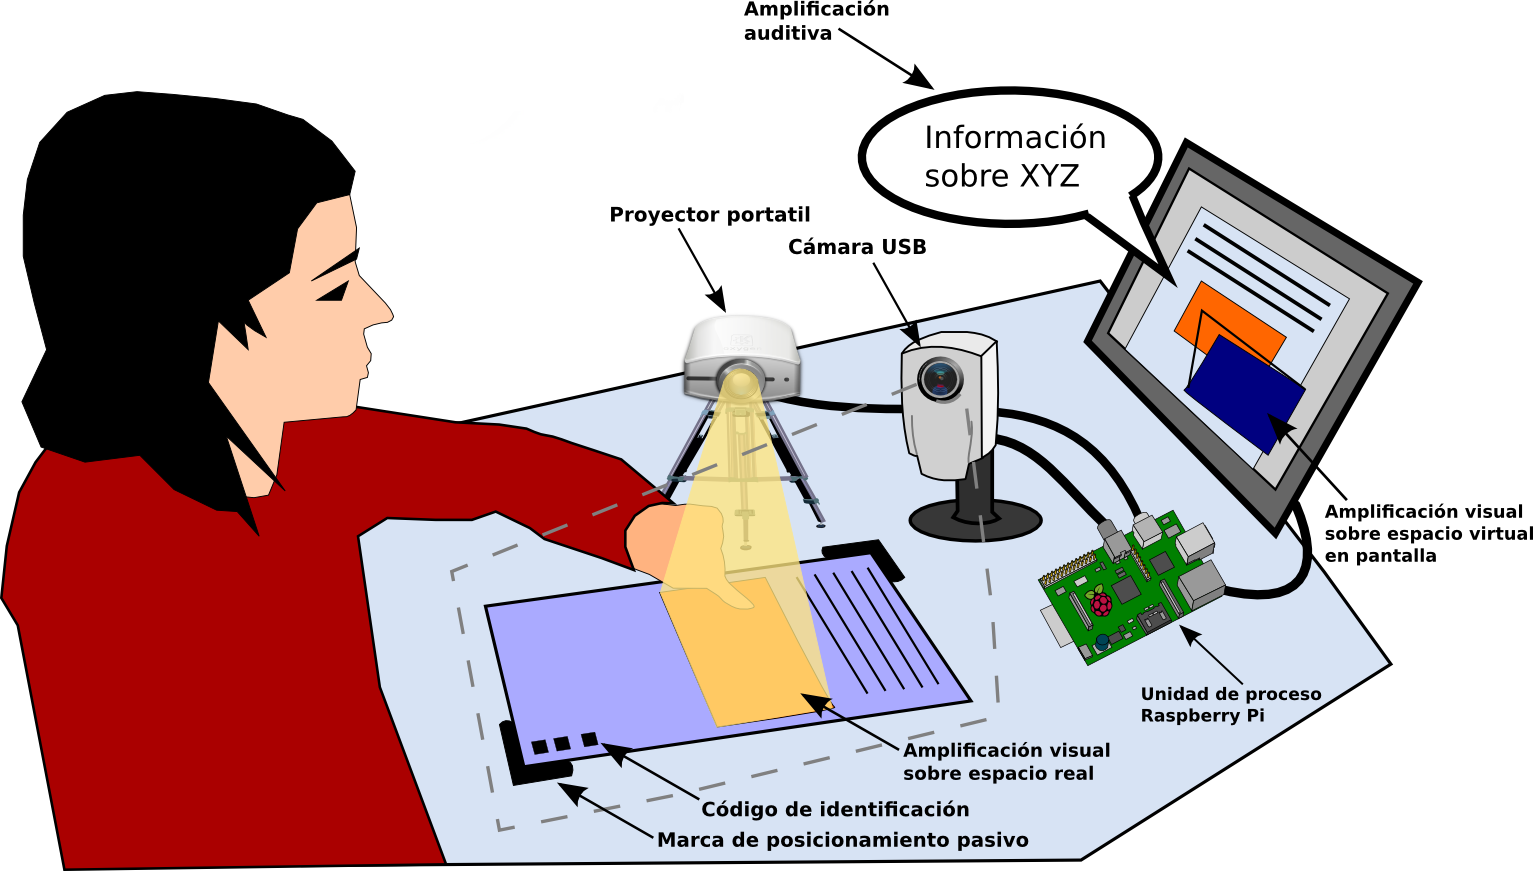
\includegraphics[width=0.85\textwidth]{argos.png}
      \caption{Esquema de componentes funcionales de ARgos}
      \label{fig:diagrama_argos}
    \end{center}
\end{figure}
   
Según lo anterior, sería deseable disponer de una herramienta que permitiera el tratamiento directo sobre estos documentos «físicos». \textit{ARgos} es, un proyecto de la Cátedra INDRA-UCLM que pretende la construcción de un sistema de ayuda a la gestión de documentos impresos mediante el uso de técnicas de visión por computador, síntesis visual y auditiva y técnicas de realidad aumentada. En la figura \ref{fig:diagrama_argos} se recogen los componentes funcionales del sistema.

%\subsection{Objetivos específicos}
GrayAR, el Trabajo Fin de Grado propuesto, abordará el desarrollo de los sistemas de captura, tracking y registro, e identificación de documentos dentro del \textit{Proyecto ARgos}, mientras que la parte de representación, delegación de tareas y scripting será realizada por Santiago Sánchez Sobrino en su TFG \textit{«BelfegAR: Plataforma para el despliegue gráfico 3D y delegación de tareas en gestión documental con realidad aumentada»}. 

\section{Objetivo general}
El objetivo general es construir sistema que utilice una cámara de bajo coste como entrada al módulo de visión por computador y un cañón de proyección portátil para mostrar información visual, directamente alineada sobre el documento del mundo físico. Responderá a las peticiones que el usuario realice sobre el espacio físico, ampliando información relacionada que sea relevante a la acción que quiera realizar. El documento podrá moverse dentro de una región del escritorio y la amplificación deberá quedar perfectamente alineada en el espacio físico. Como soporte hardware, se utilizará un computador en placa Raspberry Pi con arquitectura \acs{ARM}.

%La unidad de proceso se encargará de tomar como entrada las imágenes obtenidas por la cámara y generar la salida para el cañón de proyección. Esta salida deberá tener en cuenta el posicionamiento 3D relativo entre el documento y el cañón para que el registro de la amplificación visual sea perfecto. 

En base a este objetivo general se plantean una serie de objetivos específicos que se detallan en la siguiente sección.

\section{Objetivos específicos}

\begin{itemize}
\item \textbf{Captura y preprocesado de imágenes.} Deberemos proveer al sistema de un módulo para obtener las imágenes y aplicarle el procesado previo necesario, como puede ser el escalado, umbralización, detección de bordes o detección de características \cite{Ortiz} \cite{Bay}. Otra tarea a realizar es calcular la distorsión debida a la proyección en perspectiva mediante los parámetros extrínsecos e intrínsecos de la cámara.

\item \textbf{Sistema de identificación de documentos.} GrayAR contará con un sistema de identificación rápida empleando algoritmos de recuperación de imágenes y comparará el documento que está siendo analizado con una base de datos de documentos conocidos por el sistema.

\item \textbf{Implementación de técnicas de tracking y registro.} Para el correcto alineado de la información mostrada, el módulo de tracking y registro contará con funciones de cálculo de \emph{pose} (rotación y translación del objeto en el espacio 3D) en tiempo real y algoritmos para la estimación y descripción del movimiento como \textit{Optical Flow} \cite{LKanade}.   

\item \textbf{Utilización de paradigmas de interacción natural con el usuario (NUI).} El usuario podrá interactuar directamente en el espacio físico sin utilizar sistemas de mando o dispositivos de entrada tradicionales como sería un ratón, teclado, etc. siendo sustituidos por funciones más naturales como el uso de movimientos gestuales con las manos.

\item \textbf{Facilitar la gestión documental a personas con necesidades especiales.} Contará con diferentes modos de amplificación de la información del mundo real. Por un lado, la información visual se amplificará empleando el cañón de proyección que mostrará información relevante al contexto directamente sobre el espacio del papel, así como otras fuentes de información visual adicionales. 

\item \textbf{Se debe basar en componentes de bajo coste.} Para facilitar la implantación real en el entorno de trabajo, deberá funcionar con componentes de bajo coste, incorporando mecanismos de corrección de distorsión y registro 3D totalmente software.

\item \textbf{Dispositivo multiplataforma (hardware y software).} El desarrollo de GrayAR se realizará siguiendo estándares, tecnologías y bibliotecas libres multiplataforma, con el objetivo de que pueda ser utilizado en el mayor número de plataformas posibles tanto hardware (x86, x86-64 y ARM) como software (GNU/Linux, Windows y Mac).
\end{itemize}

% Local Variables:
%  coding: utf-8
%  mode: latex
%  mode: flyspell
%  ispell-local-dictionary: "castellano8"
% End:

%\chapter{Objectives}
\label{chap:objetivos_eng}

\drop{N}{owadays}, the largest portion of the information production of documents is carried out using IT tools. Currently, the use of the electronic signature, what guarantees the authenticity of the digital document, is being spread in the public administration, but there is still a large number of people who don't use this procedure. It is very common that in many forms, even being in digital format, documents are presented in a physical medium.

\begin{figure}[h!]
  \begin{center}
      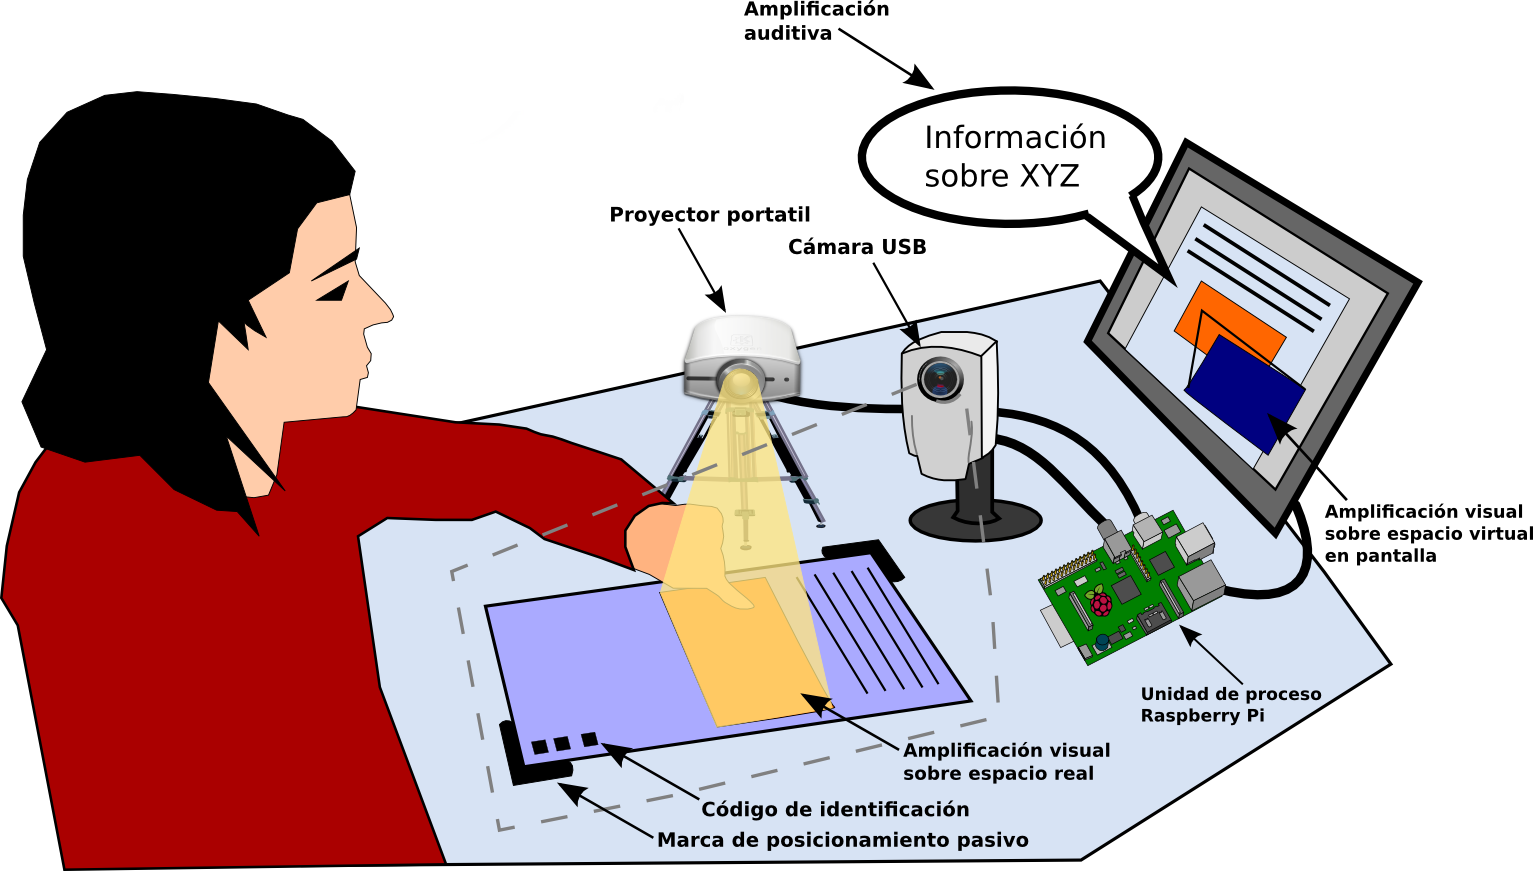
\includegraphics[width=0.85\textwidth]{argos.png}
      \caption{Functional components of \textit{ARgos}}
      \label{fig:diagrama_argos_eng}
    \end{center}
\end{figure}

According to the above, it would be desirable to have a tool that could be able to manage these \textit{«physical»} documents directly. \textit{ARgos} is an INDRA-UCLM Chairs Project that expects the construction of a support system for the management of printed documents using a computer vision system, visual and hearing synthesis and augmented reality techniques. The functional components of the system are shown in the figure \ref{fig:diagrama_argos_eng}.

GrayAR, the proposed end-of-degree project, will discuss the development of the recording, tracking and registration systems and the identification of documents that belong to the \textit{ARgos Project}, whereas the representation part, the delegation of tasks and scripting will be developed by Santiago Sánchez Sobrino in his final year work \textit{«BelfegAR: Platform for the 3D graphic display and delegation of tasks in documental management with augmented reality»}. The specific objectives to be developed are summarised below.


\section{General objective}
The general objetive is to build system that uses a low-cost camera as an input in the vision-by-computer module and a portable projection screen to show the visual information, directly aligned with the document of the physical world. It will respond to the requests done by the user in the physical space, expanding information related to the desired action. The document will be able to move in a specific region of the desktop and the amplification must be perfectly aligned in the physical area. A Raspberry Pi board with ARM architecture will be used. 
%The processing unit will take the images taken by the camera as an input and it will generate the output for the projection screen. This output must take into account the relative 3D position between the document and the projection screen to have a perfect register of the visual amplification. 

From the main objective described in the previous section, the specific objectives to be developed are summarised below.
\section{Specific objectives}
\begin{itemize}
\item \textbf{Image capture and processing.} We must provide the system with a module to obtain the images and apply a previous process, as it can be the scaling process, thresholding process, edge detection or characteristics detection  \cite{Ortiz} \cite{Bay}. Another task to be done is the calculation of the distortion due to the perspective projection using the extrinsic and intrinsic parameters of the camera. 

\item \textbf{Document image recognition system.} GrayAR will have a rapid identification system which will use image-retrieval algorithms and it will compare the document which is being analysed with a document database, known for the system. 

\item \textbf{Implementation of tracking and registration techniques.}
The tracking and registration module will have real-time pose calculation features (rotation and translation of the object in the 3D space) and algorithms to estimate and describe the movement, such as \textit{Optical Flow} \cite{LKanade}, all this to get the proper alignment of the displayed information.

\item \textbf{Use of Natural User Interface (NUI) paradigms.}
The user will directly interact with the physical space without using control systems or traditional input devices such as mouse, keyboard, etc. These devices will be replaced by natural functions such as simple gestures of the user’s hands. 

\item \textbf{Facilitation of document management for people with special needs.} GrayAR will have different ways to amplify the real world information. On the one hand, the visual information will be augmented using a projection screen that will show relevant information directly on the paper space, as well as other additional sources of visual information. 

\item \textbf{Low-cost components based.} GrayAR must operate with low-cost components to facilitate the deployment at scale, incorporating totally-software correction and 3D registration mechanisms. 

\item \textbf{Multi-platform device (hardware and software).} The GrayAR development will be made following multi-platform free standards, technologies and libraries, with the aim of using it in the largest number of possible platforms, hardware (x86, x86-64 y ARM) as well as software (GNU/Linux, Windows y Mac).
\end{itemize}
\chapter{Antecedentes}
\label{chap:antecedentes}

\drop{E}{n} este capítulo se introducirán los campos y las tecnologías relacionadas con este
proyecto, realizando una revisión de las mismas. Se realizará un estudio del estado del
arte de los sistemas existentes.

\begin{figure}[h!] 
  \centering
  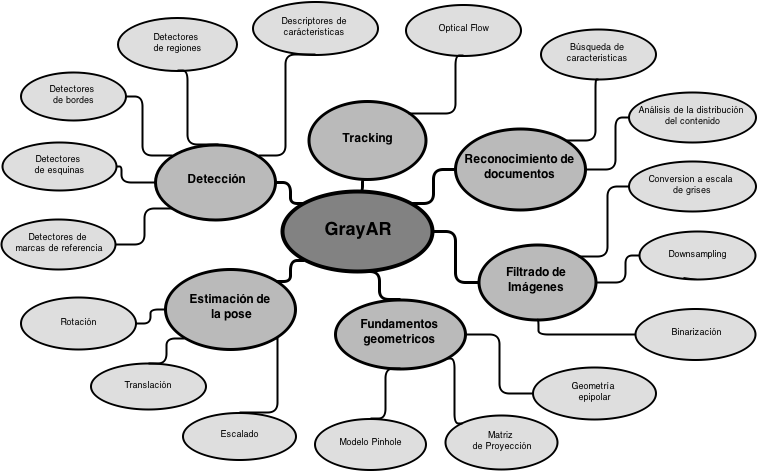
\includegraphics[width=1.0\textwidth]{conceptual_map.png}
  \caption{Antecedentes de GrayAR}
  \label{fig:antecedentes}
\end{figure}


\section{Geometría de la formación de imágenes}
La formación de las imágenes consiste en una representación bidimensional del mundo 3D, perdiéndose la información de profundidad.

La óptica geométrica clásica se basa en modelos de lentes para modelar el proceso de formación de las imágenes. Sin embargo, podemos simplificar este proceso suponiendo que todos los rayos que llegan a la cámara atraviesan un único punto y se proyectan en un plano. Este modelo se conoce como modelo \textbf{\textit{pinhole}}.

Debido a que las lentes no tienen un comportamiento ideal, habrá que añadir al modelo unos parámetros de distorsión que permitan corregirlo y aproximarlo al comportamiento real de la cámara.

\subsection{Estructura del modelo \textit{pinhole}}
El modelo \textbf{\textit{pinhole}} \cite{Hartley} permite modelar el proceso de formación de las imágenes mediante una proyección central, en la cual, de cada punto del espacio tridimensional sale un rayo de luz que pasa por un punto fijo del espacio y intersecta en un plano dando lugar a la imagen.

\begin{figure}[h]
  \centering
  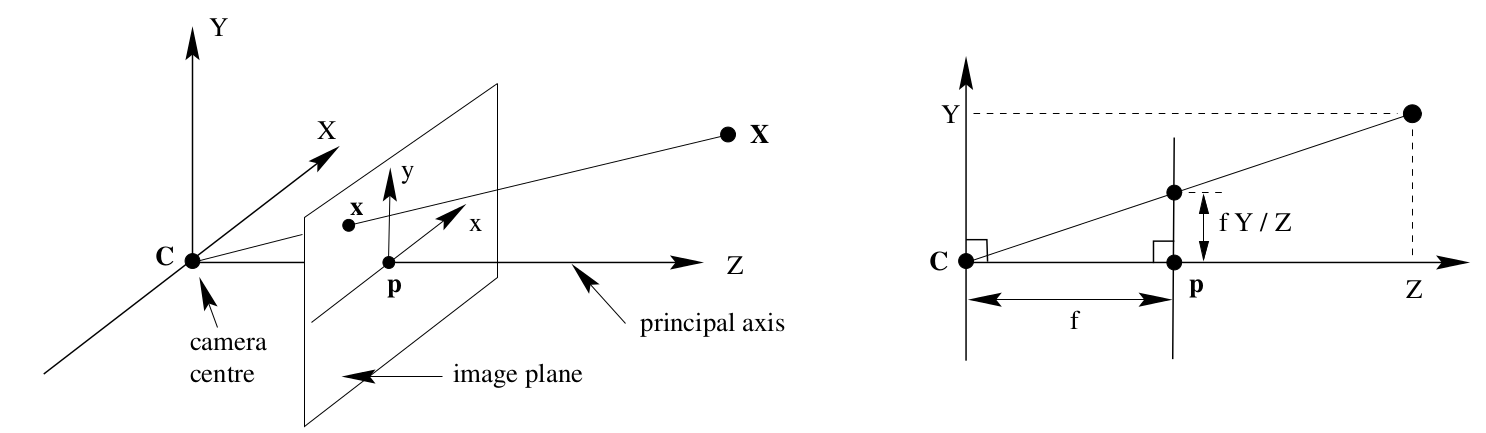
\includegraphics[width=0.85\textwidth]{pinhole.png}
  \caption{Modelo de cámara \textit{pinhole}. La imagen de un punto 3D se forma mediante proyección de perspectiva. Un punto $X$ es proyectado a un punto $x$ en el plano imagen}
  \label{fig:pinholeCamera}
\end{figure}

Los elementos que forman este modelo se definen de la siguiente forma:
\begin{itemize}
\item El \textbf{centro óptico} es el punto fijo del espacio por donde pasan todos los rayos de luz. Se corresponde con el centro de la cámara y es donde se fija el sistema de referencia de la cámara.
\item El \textbf{plano imagen} o plano focal. De cada punto del espacio parte un rayo de luz que pasa por el centro de proyección e intersecta con este plano formando la imagen. Como se puede ver en la figura, el plano focal se ha situado delante del centro óptico. Si éste estuviese detrás, las imágenes estarían invertidas.
\item \textbf{Distancia focal.} Se define como la distancia entre el centro de proyección y el plano imagen.
\item \textbf{Eje principal} Es la línea que pasa por el centro de proyección y es perpendicular al plano imagen.
\item \textbf{Punto principal.} Es el punto de intersección del eje principal con el plano imagen. Coincide con el centro de la imagen.
\item \textbf{Plano principal.} Es el plano paralelo al plano imagen y que contiene al centro de proyección. Además, este plano está formado por todos los puntos cuyas proyecciones se corresponden con puntos en el infinito en la imagen.
\end{itemize}

%Una \textbf{homografía} es una transformación proyectiva que determina una correspondencia entre dos figuras geométricas planas, de forma que a cada uno de los puntos y las rectas de una de ellas le corresponden, respectivamente, un punto y una recta de la otra.

%Una homografía es una matriz (generalmente de 3x3) cuya misión es la de mapear los puntos de una superficie planar bidimensional a otra. Según esta definición, una matriz que transforme los puntos de un plano en puntos del plano de cámara, será considerada una homografía. Esta transformación se realiza en términos de coordenadas físicas.

%\begin{figure}[tb]
%  \begin{minipage}{13.1cm}
%    \centering
%    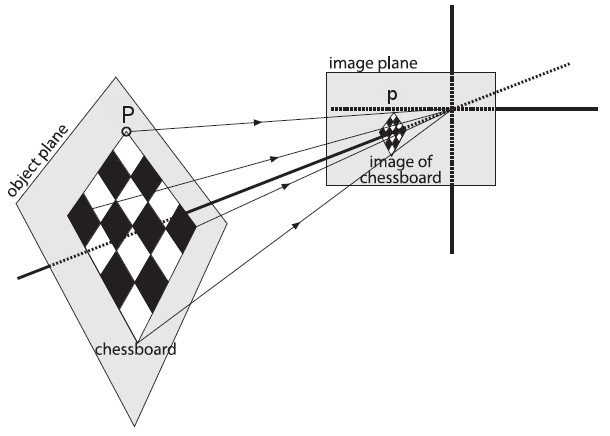
\includegraphics[width=10cm]{homografia.jpg}
%        \cite{OpenCV}.}{}}{}{\caption{Transformación de un punto P del mundo real a su proyección p
%        en el plano de cámara utilizando una homografía. (Bradski y Kaehler)}}
%    \ifthenelse{\equal{FIGhomografia}{}}{}{\label{FIGhomografia}}
%  \end{minipage}
%\end{figure}

%Se ha introducido el parámetro $s$, el cual es un factor de escala arbitrario (entendiéndose que la homografía está definida bajo ese factor, debido al desconocimiento de las medidas del mundo real). En la figura \ref{FIGhomografia} puede verse la implicación de utilizar la homografía en este escenario.

%Podría llegar a pensarse que las funciones de la matriz esencial y de la homografía son las mismas,
%puesto que ambas realizan transformaciones en la geometría del sistema de visión estereoscópica sin tener en cuenta los parámetros intrínsecos de la cámara. La diferencia reside en que la homografía trabaja sobre planos que son visibles desde la cámara y relacionaría un punto de ese plano con el de su propio plano. La matriz esencial no tiene en cuenta esta restricción y solo es capaz de relacionar un punto en una imagen que se encuentre alineado con otra imagen.

\subsection{Matriz de proyección}\label{subsec:matproy}
El modelo \textit{pinhole} \cite{Hartley} fija un sistema de coordenadas proyectivas en el centro óptico. El eje $Z$ de este sistema coincide con el eje principal de la cámara. A partir de ahora nos referiremos a este sistema de coordenadas como sistema de referencia de la cámara. Además, el plano imagen se fija en el plano $Z = f$.

\begin{figure}[h]
  \centering
  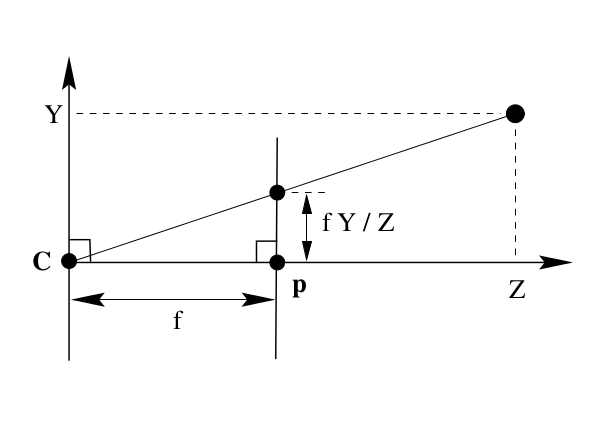
\includegraphics[width=0.8\textwidth]{pinhole2.png}
  \caption{Modelo de cámara \textit{pinhole} visto desde el eje $X$}
  \label{fig:pinholeCamera2}
\end{figure}

Utilizaremos $[X, Y, Z]$, para representar vectores fila. Por tanto, su traspuesta, $[X, Y, Z]^T$, será un vector columna. 

Por convenio con la notación anterior, las coordenadas de un punto cualquiera se van a representar por un vector columna, definiendo los siguiente elementos a considerar:
\begin{itemize}
\item $[X_c , Y_c , Z_c ]^T$ Coordenadas de un punto del espacio tridimensional respecto al sistema de referencia de la cámara.
\item $[X_w , Y_w , Z_w ]^T$ Coordenadas del mismo punto del espacio tridimensional respecto a un sistema de referencia asociado al modelo del objeto. Este nuevo sistema de referencia es distinto al de la cámara.
\item $[x, y]^T$  Coordenadas del punto proyectado en el plano imagen.
\item $f$  Distancia focal
\end{itemize}

Mediante relación de semejanza de triángulos, de la figura \ref{fig:pinholeCamera2}: 
\begin{equation}\label{eq:semejanza}
\dfrac{x}{f} = \dfrac{X}{Z} \quad \quad \quad \quad \dfrac{y}{f} = \dfrac{Y}{Z} 
\end{equation}

podemos determinar la correspondencia entre un punto cualquiera del espacio y su proyección en el plano imagen:
\begin{equation}\label{eq:proyeccion}
  (X_c , Y_c , Z_c )^T \Longrightarrow  (x, y)^T = (f \dfrac{X_c}{Z}, f \dfrac{Y_c}{Z})^T
\end{equation}

Las \textbf{coordenadas homogéneas} son un instrumento empleado para describir un punto en el espacio proyectivo. Consiste en ampliar el plano euclídeo (en el caso bidimensional) al plano proyectivo, es decir, incluirle los puntos impropios o del infinito. De forma que, un punto de dimensiones $(x, y, z)$, se representa por la terna: $(x/w$, $y/w$, $z/w)$ con $w=1$. %Y un punto impropio es aquel donde $w=0$.

Este sistema de coordenadas tiene la particularidad de que permite pasar fácilmente coordenadas de un número de dimensiones a otro. Para ello, almacena las coordenadas con una dimensión adicional, de tal forma que para un espacio de 3D, utilizaríamos 4 coordenadas. El valor de la coordenada adicional indica entre otras cosas, si el punto se encuentra en el infinito, $w=0$, o es un punto cualquiera, $w \neq 0$. En este sistema, si dos coordenadas son proporcionales, se refieren al mismo punto.

Utilizándolas, podemos expresar un punto del espacio tridimensional respecto al sistema de referencia de la cámara de forma matricial:
\begin{equation} 
\begin{pmatrix}
    X_{c} \\
    Y_{c} \\
    Z_{c} \\
    1
  \end{pmatrix}
  \Longrightarrow
  \begin{pmatrix}
    fX_{c} \\
    fY_{c} \\
    Z_{c} \\
  \end{pmatrix}
  =
  \begin{bmatrix} f & 0 & 0 & 0 \\ 0 & f & 0 & 0 \\ 0 & 0 & 1 & 0 \\\end{bmatrix}
  \begin{pmatrix} X_{w} \\  Y_{w} \\  Z_{w} \\  1 \\\end{pmatrix}
\end{equation}
y la expresión de relación de correspondencia, queda de la siguiente forma:
\begin{equation} 
\begin{pmatrix}
    X_{w} \\
    Y_{w} \\
    Z_{w} \\
    1
  \end{pmatrix}
=
  \begin{bmatrix} f & 0 & 0 & 0 \\ 0 & f & 0 & 0 \\ 0 & 0 & 1 & 0 \\\end{bmatrix}
  \begin{pmatrix} X_{c} \\  Y_{c} \\  Z_{c} \\  1 \\\end{pmatrix}
\end{equation}

Y de forma abreviada:

\begin{equation}\label{eq:proy}
\overline{x_w} = P \overline{X_c}   
\end{equation}
donde:
\begin{itemize}
\item $P = diag(f, f, 1) [I|0]$
\item $diag(f, f, 1)$ es una matriz diagonal.
\item $[I|0]$ representa una matriz identidad de 3x3 concatenada con un vector columna nulo de dimensión 3.
\item $\overline{X_c}$  es el vector columna, de dimensión 4, que representa las coordenadas homogéneas del punto del espacio respecto al sistema de referencia de la cámara.
\item $\overline{x}$  es el vector columna, de dimensión 3, que representan las coordenadas homogéneas del punto de la imagen.
\item A la matriz $P$ de se la denomina \textbf{matriz homogénea de proyección de la cámara}.
\end{itemize}


\subsection{Parámetros intrínsecos de la cámara}
La matriz de proyección $P$ de la ecuación \ref{eq:proy} permite transformar las coordenadas de un punto 3D del mundo real en píxeles de una imagen. Se construye a partir de una matriz $K$ y un vector de valores nulos:
\begin{equation}
 P = [K|0] 
\end{equation}
donde la $K$ es la \textbf{matriz de la cámara}, la cuál está formada por una serie de parámetros, denominados \textbf{parámetros intrínsecos}:

\begin{equation}
  K =
  \begin{bmatrix}
    f_{x} & \gamma & {c_{x}} \\
    {0}&{f_{y}}&{c_{y}}\\
    {0}&{0}&{1}
  \end{bmatrix}
\end{equation}

Los \textbf{parámetros intrínsecos} son aquellos que describen las características ópticas y geométricas de una cámara y son constantes. Entre estos parámetros se encuentran la distancia focal, el centro óptico y el punto principal. En la figura \ref{fig:FIGparamCam} se pueden visualizar estos tres parámetros.

\begin{figure}[h]
  \centering
  \includegraphics[width=0.7\textwidth]{parametrosCamara.pdf}
  \caption{Parámetros intrínsecos de una cámara.}
  \label{fig:FIGparamCam}
\end{figure}

\begin{itemize}
\item El \textbf{centro óptico} o centro de proyección, es el punto de la cámara desde el cual parten todos los rayos que son proyectados en el plano de imagen de la cámara.

\item El \textbf{punto principal}, denotado como \textbf{\textit{c}}, es la proyección ortogonal del centro óptico sobre el plano de cámara.  $c_x$, $c_y$ indican el desplazamiento del centro de coordenadas del plano imagen, respecto al punto principal. Será nulo sólo si el eje óptico coincide con el centro del sensor de la cámara, pero el eje óptico no siempre atraviesa el centro de la imagen generada. 

\item El \textbf{factor $\gamma$ (\textit{skew factor})} determina el grado de perpendicularidad de las paredes de los píxeles del sensor. Es inversamente proporcional a la tangente del ángulo que forman los ejes $X$ e $Y$, por lo que  $\gamma$ tendrá un valor nulo si los píxeles son rectangulares. Esto suele ser así en casi todos los sensores utilizados hoy en día. 

\item La \textbf{distancia focal}, es la distancia existente entre el centro óptico y el punto principal. $f_x$ y $f_y$ son dos distancias focales en píxeles. Son proporcionales a la longitud focal $f$ considerada en las ecuaciones (\ref{eq:semejanza}) y (\ref{eq:proyeccion}), según 
\begin{equation}
f_x = f S_x \quad \quad  \quad \quad f_y = f S_y
\end{equation}
donde: $f$ es la longitud focal física de la lente, en unidades de longitud (milímetros, micras, etc.). $S_x$ y $S_y$ son el número de píxeles por unidad de longitud del sensor, a largo del eje $X$ y del eje $Y$ respectívamente. Como es obvio, si el sensor tiene el mismo número de píxeles por unidad de longitud en todas sus dimensiones, las dos focales $f_x$ y $f_y$ tendrán el mismo valor.
\end{itemize}

\subsection{Distorsión}
El uso de lentes facilita la entrada de luz, un enfoque adecuado y una mayor versatilidad, pero también introduce deformaciones en las imágenes que se forman en el sensor. Para el cálculo de coeficientes de distorsión, se tienen en cuenta factores radiales y tangenciales. 

La \textbf{distorsión radial}, consiste en el desplazamiento de los píxeles de de la imagen, de tal modo que las líneas situadas en los extremos del encuadre aparentarán salir hacia el exterior o el interior.   

Para la correción de la distorsión radial de las coordenadas de un pixel de la imagen, se utiliza la siguiente fórmula:
\begin{equation}
  \begin{split}
    x_{corrected} = x(1 + k_1 r^2 + k_2 r^4 + k_3 r^6)  \\
    y_{corrected} = y(1 + k_1 r^2 + k_2 r^4 + k_3 r^6)
  \end{split}
\end{equation}

La \textbf{distorsión tangencial} se produce porque la lente no se encuentra perfectamente paralela al plano de imagen. Se puede corregir a través de las siguientes fórmulas:
\begin{equation}
  \begin{split}
    x_{corrected} = x + [ 2p_1xy + p_2(r^2+2x^2)] \\ 
    y_{corrected} = y + [ p_1(r^2+ 2y^2)+ 2p_2xy]
  \end{split}
\end{equation}

%Por otra parte, se obtiene un vector con los factores de distorsión de la cámara. Normalmente este vector contiene 5 valores, correspondientes a 3 factores de distorsión radial, denotados como $k_{i}$ y 2 factores de distorsión tangencial, denotados como $p_{j}$. El número de factores de distorsión radial puede verse incrementado hasta 5, dependiendo del algoritmo de calibración que se realice.
De tal forma que tenemos cinco parámetros de distorsión que son representados en OpenCV como una matriz fila con 5 columnas: 

\begin{equation}
  Distortion_{coefficients} = [k_1 \hspace{10pt} k_2 \hspace{10pt} p_1 \hspace{10pt} p_2 \hspace{10pt} k_3]
\end{equation}

% \begin{figure}[h!]
%   \ifodd\thepage\hspace{-5.2cm}\else\hspace{-0.1cm}\fi\begin{minipage}{13.1cm}
%     \centering
%     \includegraphics[width=9cm]{extrinsicCamara}
%     \ifthenelse{\equal{Transformación geométrica dada por los parámetros extrínsecos entre la posición inicial y final de una cámara. Imagen: \textit{Learning OpenCV} \cite{OpenCV}}{}}{}{\caption{Transformación geométrica dada por los parámetros extrínsecos entre la posición inicial y final de una cámara. Imagen: \textit{Learning OpenCV} \cite{OpenCV}}}
%     \ifthenelse{\equal{FIGextrinsicCam}{}}{}{\label{FIGextrinsicCam}}
%   \end{minipage}
% \end{figure}

\subsection{Parámetros extrínsecos de la cámara}
En la sección \ref{subsec:matproy} se asumió el hecho de que el centro óptico era el origen de coordenadas del mundo. Esto era así a efectos del cálculo de parámetros intrínsecos, con lo cual el modelo era válido siempre que el sistema no fuera movido de su posición inicial.

Por otro lado, en la mayor parte de las aplicaciones prácticas es necesario que la cámara se mueva o se gire, para captar adecuadamente la escena. Por ello, para poder modelar el sistema con independencia de que su posición haya sido alterada o de que un objeto se pueda referenciar respecto al origen de coordenadas de la cámara, es necesario modificar la ecuación \ref{eq:proy} introduciendo un matriz de transformación $[R|t]$ que contiene los \textbf{parametros extrínsecos} de la cámara. 

\begin{equation}
x = K [R|t] X  
\end{equation}

\begin{figure}[h!]
  \centering
  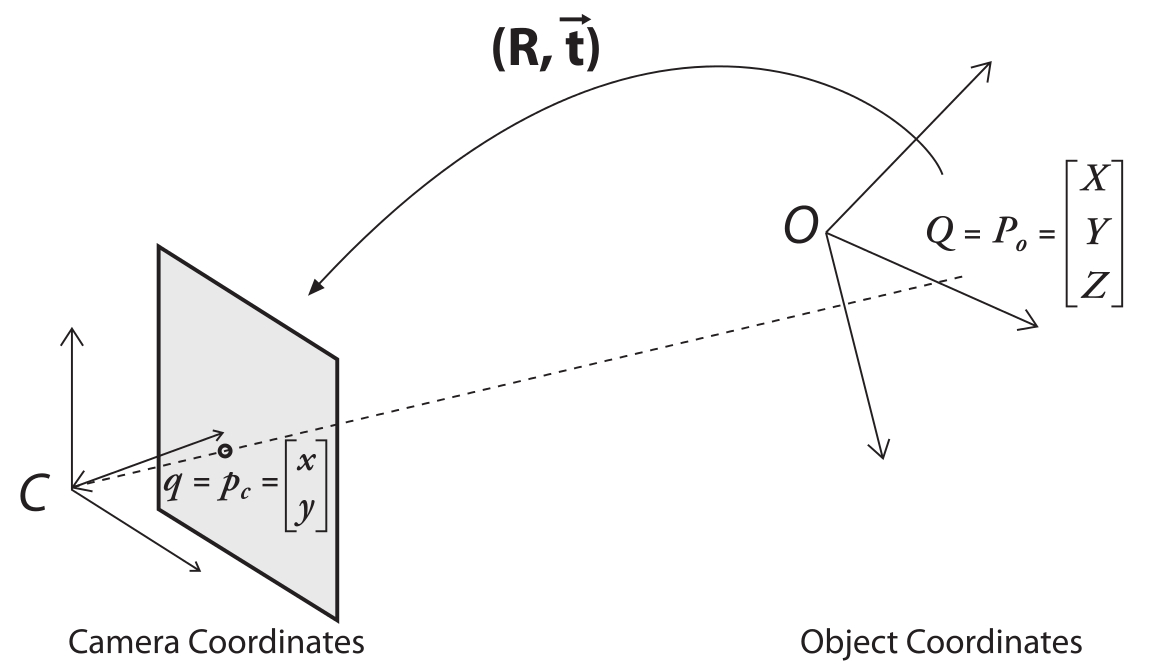
\includegraphics[width=0.80\textwidth]{rt.png}
  \caption{Conversión del sistemas de coordenadas del objeto al sistema de la cámara. El punto $p_c$
    está relacionado con el punto $P_0$ mediante la aplicación de una la matriz de rotación y el
    vector de traslación. (Bradski y Kaehler)}
  \label{fig:RT}
\end{figure}

\begin{equation}
  [R|t] = 
  \begin{bmatrix} 
    R_{1,1} & R_{1,2} & R_{1,3} & T_{1}  \\
    R_{2,1} & R_{2,2} & R_{2,3} & T_{2}  \\
    R_{3,1} & R_{3,2} & R_{3,3} & T_{3}  \\
    0      &   0    &   0   &  1
  \end{bmatrix}
\end{equation}

Donde: 
\begin{itemize}

\item $R$ es una \textbf{matriz de rotación}, que representa un giro de la cámara (o de un objeto respecto de ella). Tendrá una forma distinta dependiendo de respecto a que eje (X, Y, Z) se haga la rotación:
\begin{equation}
R_x(\Psi)=\begin{bmatrix}
1 & 0         & 0        \\ 
0 & \cos\Psi  & \sin\Psi \\ 
0 & -\sin\Psi & \cos\Psi
\end{bmatrix}
\end{equation}

\begin{equation}
R_y(\varphi)=\begin{bmatrix}
\cos\varphi & 0 & -\sin\varphi \\ 
0           & 1 & 0            \\ 
\sin\varphi & 0 & \cos\varphi
\end{bmatrix}
\end{equation}

\begin{equation}
R_z(\theta)=\begin{bmatrix}
\cos\theta  & \sin\theta & 0 \\ 
-\sin\theta & \cos\theta & 0 \\ 
0           & 0          & 1
\end{bmatrix}
\end{equation}

Si el giro se realiza respecto al eje $Z$, tal y como se muestra en la figura \ref{fig:rotatingPoints}, las nuevas coordenadas quedarán de la siguiente forma:

\begin{figure}[h]
  \centering
  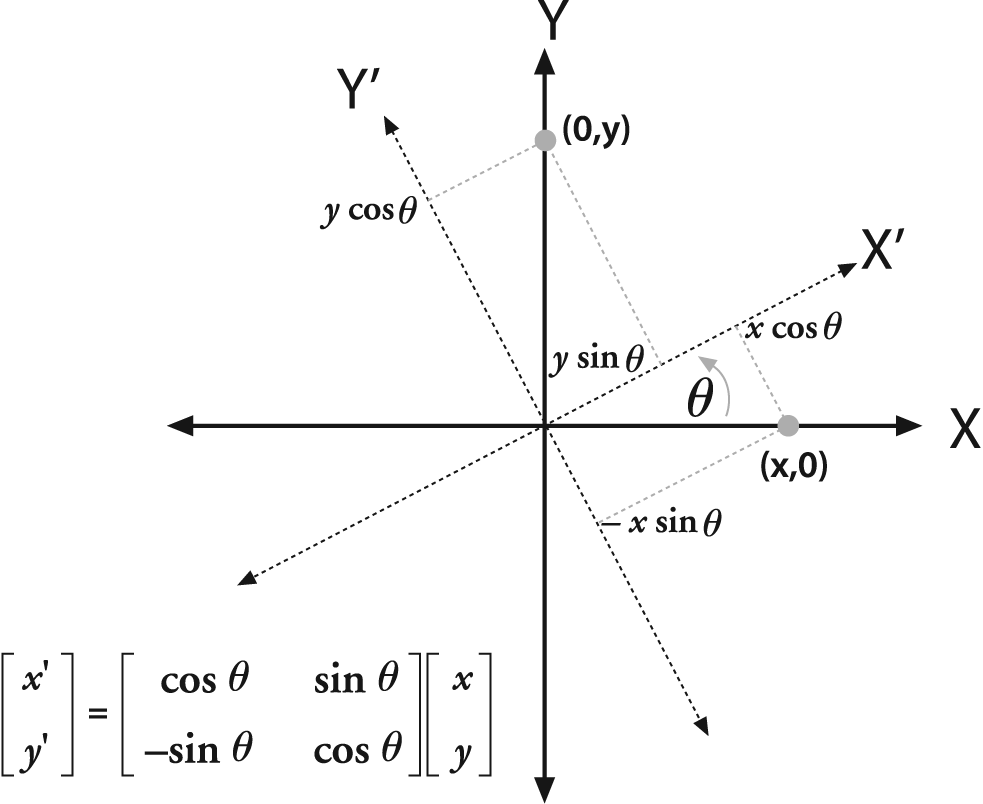
\includegraphics[width=0.6\textwidth]{rotatingPoints.png}
  \caption{Rotación de puntos alrededor del eje Z (Bradski y Kaehler)}
  \label{fig:rotatingPoints}
\end{figure}

\begin{equation}
\begin{bmatrix}
X'\\ 
Y'\\ 
Z'
\end{bmatrix}
=
\begin{bmatrix}
\cos\theta  & \sin\theta & 0 \\ 
-\sin\theta & \cos\theta & 0 \\ 
0           & 0          & 1
\end{bmatrix}
\begin{bmatrix}
X\\ 
Y\\ 
Z
\end{bmatrix}
\Rightarrow 
\begin{aligned}
X'&= X\cos\theta + Y \sin\theta \\ 
Y'&=-X\sin\theta + Y \cos\theta \\ 
Z'&= Z
\end{aligned}
\end{equation}

\item $t$ es un \textbf{vector de translación} que representa el cambio de un sistema de coordenadas a otro cuyo origen se desplaza a otra ubicación; en otras palabras, el vector de traslación es el desplazamiento desde el origen del sistema de coordenadas inicial hasta el origen del sistema de coordenadas final. En nuestro caso, como podemos ver en la figura \ref{fig:RT}, el sistema inicial pertenecería al del objeto, y el final, al sistema de coordenadas de la cámara. 
\begin{equation}
t = origen_{objeto} - origen_{camara}
\end{equation}


\end{itemize}

El cálculo aproximado de la matriz de transformacion $[R|t]$ a partir de la información visual capturada se denomina \textbf{\textit{pose estimation}}. La solución para la estimación de la \textit{pose} ha sido propuesta, entre otros métodos, mediante transformada lineal directa (DLT) ó algoritmos Pnp (perspective-n-point).

%Tanto la matriz de cámara como el vector de distorsión contienen únicamente parámetros intrínsecos, lo que significa que serán constantes. No ocurre lo mismo con los parámetros extrínsecos, que varían en función de la situación de la cámara en el escenario, y que producen una matriz de rotación y un vector de traslación. Estos dos elementos indican la transformación geométrica que hay que realizar sobre la cámara para alcanzar la posición y la rotación finales desde su posición inicial. En la figura \ref{fig:RT} se puede ver gráficamente la implicación de los parámetros extrínsecos.

%Los \textbf{parámetros extrínsecos} son aquellos que definen la posición y la orientación de la cámara con respecto al mundo real.

%Comúnmente, para la determinación de estos parámetros significa:
%\begin{itemize}
%\item Encontrar el \textbf{vector de translación} entre las posiciones relativas al origen de dos sistemas de referencia.
%\item Encontrar la \textbf{matriz de rotación} que provocan los ejes correspondientes a los dos sistemas de referencia alineados ( ej.: uno sobre otro)
%\end{itemize}

%El proceso de estimación de pose de un objeto consiste en determinar los parámetros de rotación y translación de dicho objeto a partir de información visual. %El problema se consolida como uno de los retos más destacados en el campo de la visión por computador, surgiendo numerosas alternativas y métodos para solucionarlo.

%La pose del objeto viene determinada por una posición (3 parámetros: X, Y, Z) y una orientación (3 ángulos: yaw, pitch, roll) que forman un conjunto de 6 grados de libertad (6DOF). La solución para la estimación de la pose ha sido propuesta, entre otros métodos, mediante transformada lineal directa (DLT), algoritmos Pnp (perspective-n-point).

%El objetivo es encontrar una correspondencia entre puntos de la imagen en 2D y sus coordenadas en el mundo 3D. A la hora de representar los objetos del espacio observado (3D), los convertimos a un plano de visión (2D), y tenemos que definir cual es la correspondencia entre las coordenadas del espacio y las de la representación. Para facilitar esta conversión, se utiliza el sistema de coordenadas ``homogéneo''. 

%Las matrices de transformación, utilizadas para pasar de unas dimensiones a otras, suelen incluir 3 tipos de transformaciones \textbf{R}otación, \textbf{T}ranslación y e\textbf{S}calado. Podemos representarlas así:

%Para convertir las coordenadas del mundo a coordenadas de pantalla, de espacio tridimensional a bidimensional, los sistemas de visión artificial utilizan la siguiente fórmula:
%\begin{equation}
%q=MQ
%\end{equation}
%donde:
%\begin{center}
%$q=\begin{bmatrix} x \\ y \\ z \end{bmatrix}$, $M=\begin{bmatrix} f_{x} & 0 & c_{x} \\ 0 & f_{y} & c_{y} \\ 0 & 0 & 1 \end{bmatrix}$ y %$Q=\begin{bmatrix} X \\ Y \\ Z \end{bmatrix}$
%\end{center}

%Por tanto, $q$ representa el espacio bidimensional en coordenadas homogéneas, y $Q$ el espacio tridimensional. $f_{x}$ es la distancia focal en el eje $X$, $f_{y}$ la distancia focal en el eje $Y$, ($c_{x},c_{y}$) marcan el punto principal, el punto donde el eje de visión corta el plano de visión (normalmente suele estar en el centro de la imagen, o muy cerca)

%Mediante alguna técnica de resolución al problema PnP, se calcula la pose (rotación y traslación) dado un conjunto de puntos de objeto, sus proyecciones en la imagen correspondiente, así como la matriz de cámara y los coeficientes de distorsión. Esta función encuentra una pose que minimiza el error de reproyección, es decir, la suma de los cuadrados de las distancias entre las proyecciones observados y las puntos proyectados
%La matriz de la cámara se corresponde con sus parámetros intrínsecos. Tanto la matriz como el vector de coeficientes de distorsión se obtienen en un proceso previo de calibración de la cámara y se mantienen fijos y conocidos durante todo el proceso.


%usando los parámetros extrínsecos de la cámara, podemos encontrar la relación entre las coordenadas de un punto $P$ en el mundo $(P_w)$ y las coordenadas de la cámara %$\left(P_c\right)$:
%\begin{equation}
%  P_c=R\left(P_w-T\right)where R=\begin{pmatrix}
%    r_{11} & r_{12} & r_{13}\\
%    r_{21} & r_{22} & r_{23}\\
%    r_{31} & r_{32} & r_{33}
%  \end{pmatrix}
%\end{equation}

%Si $P_c=\begin{pmatrix}{X_c} \\ {Y_c} \\ {Z_c} \end{pmatrix}$ Y $P_w=\begin{pmatrix}{X_w} \\ {Y_w} \\ {Z_w} \end{pmatrix}$, entonces
%\begin{equation}
%  \begin{pmatrix} X_{c}\\ Y_{c}\\ z_{c}\end{pmatrix} =\begin{pmatrix}r_{11} & r_{12} & r_{13}\\r_{21} & r_{22} & r_{23}\\r_{31} & r_{32} & r_{33}
%  \end{pmatrix}\begin{pmatrix}X_{w} - T_{x}\\Y_{w} - T_{y}\\Z_{w} - T_{z}\end{pmatrix}
%\end{equation}
%o
%\begin{equation}
%  X_c=R^{T}_1\left(P_w-T\right)\\
%  Y_c=R^{T}_2\left(P_w-T\right)\\
%  Z_c=R^{T}_3\left(P_w-T\right)
%\end{equation}
%donde $R^{T}_i$ corresponde a la fila $i-th$ de la matriz de rotación.



%\begin{figure}[h!]
%  \centering
%  \includegraphics[width=0.6\textwidth]{extrinsicCamara}
%  \caption{Transformación geométrica dada por los parámetros extrínsecos entre la posición inicial y final de una cámara.}
%  \label{fig:FIGextrinsicCam}
%\end{figure}

%\subsection{Combinación de parámetros extrínsecos e intrínsecos de la cámara}

%La matriz que contiene los parámetros intrínsecos de la cámara:
%\begin{equation}
%  M_{in}=\begin{pmatrix}-\frac{f}{s_x} & 0 & 0_{x}\\0 & -\frac{f}{s_y} & o_y\\0 & 0 & 1\end{pmatrix}
%\end{equation}
%- La matriz que contiene los parámetros extrínsecos de la cámara:
%\begin{equation}
% M_{ex}=\begin{pmatrix}r_{11} & r_{12} & r_{13} & -R_1^TT\\r_{21} & r_{22} & r_{23} & -R_2^TT\\r_{31} & r_{32} & r_{33} & -R_3^TT\end{pmatrix}M_{ex}=\begin{pmatrix}r_{11} & r_{12} & r_{13} & -R_1^TT\\r_{21} & r_{22} & r_{23} & -R_2^TT\\r_{31} & r_{32} & r_{33} & -R_3^TT\end{pmatrix}
%\end{equation}

%Usar coordenadas homogéneas:
%\begin{equation}
%  \begin{pmatrix}x_{h}\\y_{h}\\w \end{pmatrix}=M_{in}M_{ex}\begin{pmatrix}x_{w}\\y_{w}\\z_{w}\\1 \end{pmatrix}=M\begin{pmatrix}x_{w}\\y_{w}\\z_{w}\\1 \end{pmatrix}=\begin{pmatrix}m_{11} &m_{12} & m_{13} & m_{14}\\m_{21} & m_{22} & m_{23} & m_{24}\\m_{31} & m_{32} & m_{33} & m_{34}\\m_{41} & m_{42} & m_{43} & m_{44}\end{pmatrix}\begin{pmatrix}x_{w}\\y_{w}\\z_{w}\\1 \end{pmatrix}
%\end{equation}
%
%La homogeneización es necesaria pra obtener las coordenadas píxel:
%\begin{equation}
%  x_{im}=\frac{x_h}{w}=\frac{m_{11}X_w+m_{12}Y_w+m_{13}Z-w+m_{14}}{m_{31}X_w+m_{32}Y_w+m_{33}Z-w+m_{34}}
%  y_{im}=\frac{y_h}{w}=\frac{m_{21}X_w+m_{22}Y_w+m_{23}Z-w+m_{24}}{m_{31}X_w+m_{32}Y_w+m_{33}Z-w+m_{34}}
%\end{equation}

%Llamamos M a la proyección de la matriz (es una matriz 3x4)
%
%Nota: la relación de los puntos 3D y sus proyecciones 2D pueden ser vistas como una transformación lineal de la proyección espacial $({X_w}, {Y_w}, {Z_x}, 1)^T$ a la proyección del plano $({X_h}, {Y_h}, w)^T$.


%\subsection{Visión Estereoscópica}

%Un proyector se calibra usando los mismos algoritmos de calibración que una cámara ya que puede considerarse como una ``cámara inversa''. No obstante el hecho de poder aplicar un modelo pin-hole a un proyector no parece tan evidente como en el caso de una cámara. Para la calibración de un proyector es inevitable el uso al menos una cámara. Para calibrar un proyector, ya sea usando el método de Tsai \cite{Tsai}, como el método de Zhang \cite{Zhang99} es necesario obtener un conjunto de coordenadas 3D-2D correspondientes. La \textbf{Visión Estereoscópica} consiste en el empleo de dos vistas del mismo espacio desde diferentes puntos de visionado.

%\subsubsection{Geometría epipolar}

%La geometría más básica en la que se basa cualquier sistema de visión estereoscópica es la \textbf{geometría epipolar}. Se parte de la base de que en un sistema geométrico de este tipo se tienen una cámara izquierda y una cámara derecha.

%\begin{figure}
%  \centering
%  \includegraphics[width=0.7\textwidth]{geometriaEpipolar.pdf}
%  \caption{Elementos básicos de la geometría epipolar.}
%  \label{fig:FIGgeomEpipolar}
%\end{figure}

%En la figura \ref{fig:FIGgeomEpipolar} se pueden observar los elementos que componen la geometría epipolar de un sistema estereoscópico. A cada cámara le corresponde un centro de proyección, denotados como $O_{l}$ y $O_{r}$, y un plano proyectivo, $\Pi_{l}$ y $\Pi_{r}$. El punto P, perteneciente al mundo físico tiene una proyección dentro de cada uno de los planos proyectivos. A estas proyecciones se las denomina como $p_{l}$ y $p_{r}$.

%Unos puntos geométricos importantes aquí son los llamados \textbf{epipolos}. Un epipolo $e_l$ (res\-pectivamente $e_r$) en un plano de imagen $\Pi_{l}$ (respectivamente $\Pi_{r}$) se define como la imagen del centro de proyección de la otra cámara $O_{r}$ (respectivamente $O_{l}$). Teniendo presentes estos elementos, existe un plano formado entre el punto P y los dos epipolos $e_{l}$ y $e_{r}$ denominado \textbf{plano epipolar}. Las líneas $p_{l}e_{l}$ y $p_{r}e_{r}$ (líneas que atraviesan los centros de proyección y los correspondientes epipolos), se llaman \textbf{líneas epipolares}.

%Para poder entender la utilidad de estos elementos se parte de que el punto P es visto en la cámara de la derecha. Debido a que la cámara solo ve $p_{r}$ (la proyección de P en $\Pi_{r}$), el punto P podría estar localizado en cualquier lugar de la línea definida por $p_{r}$ y $O_{r}$. Obviamente, esta línea contiene P, pero también contiene un gran número de puntos. Lo interesante de esto es que esta línea se encuentra proyectada en el plano de la imagen izquierda $\Pi_{l}$; de hecho, esa proyección es lo que antes ha sido definido como línea epipolar.

%Con este escenario, pueden extraerse una serie de propiedades:

%\begin{itemize}
%\item Todo punto 3D visto por ambas cámaras está contenido en el plano epipolar que intersecta cada imagen en una línea epipolar.
%\item Dado un punto 2D en una imagen, su punto asociado en la otra imagen se encuentra a lo largo de la correspondiente línea epipolar. Esto es lo que se conoce como \textbf{restricción epipolar}.
%\item La restricción epipolar implica que la búsqueda bidimensional de puntos asociados entre dos vistas se convierte en una búsqueda unidimensional a través de las líneas epipolares una vez conocida la geometría epipolar del sistema estereoscópico.
%\end{itemize}


%\subsubsection{Fundamentos matemáticos}

%Una vez conocidos los elementos que describen un sistema estereoscópico, se mostrará la utilización de dos matrices a través de las cuales pueden realizarse transformaciones sobre el sistema estereoscópico. Estas matrices son la \textit{matriz esencial} y la \textit{matriz fundamental}.

%\subsubsection{La matriz esencial}

%Se define la matriz esencial ($E$) de un sistema estereoscópico como aquella que contiene la información de traslación y rotación que relaciona las dos cámaras en el espacio físico.

%Esto significa que, conocidas las coordenadas de un punto $p_{l}$ en la imagen izquierda, puede conocerse su punto correspondiente en la imagen derecha $p_{r}$ multiplicando dicho punto por la matriz esencial del sistema, de tal forma que se cumple la siguiente ecuación:

%\begin{equation}
%  p_{r}^TEp_{l} = 0
%  \label{esencial}
%\end{equation}\\
%Es importante indicar que la matriz esencial no tiene en cuenta los parámetros intrínsecos de la cámara, por ello es por lo que trabaja en coordenadas físicas.

%\subsubsection{La matriz fundamental}

%La matriz esencial contiene toda la información acerca de la geometría de una cámara con respecto de la otra, pero no posee información de las cámaras en sí. En la práctica resulta más útil trabajar en unidades de píxel, ya que estas son las que se conocen en primera instancia al trabajar con imágenes.

%Para conocer la relación entre un píxel en una imagen y su píxel correspondiente en la otra imagen a través de la linea epipolar debe introducirse información de los parámetros intrínsecos de las cámaras. Para hacer esto, cada punto $p$ se sustituye por $q$, aplicando la matriz de cámara al anterior punto $p$, de tal forma que $q=Mp$, o, de forma equivalente, $p=M^{-1}q$. De esta forma, la ecuación \ref{esencial} se convierte en:

%\begin{equation*}
%  q_r^T(M_r^{-1})^TEM_l^{-1}q_l=0
%\end{equation*}\\
%Partiendo de esto, se define la matriz fundamental $F$ como:

%\begin{equation}
%  F=(M_r^{-1})^TEM_l^{-1}
%  \label{defFundamental}
%\end{equation}\\
%Sustituyendo:

%\begin{equation}
%  q_r^TFq_l=0
%  \label{fundamental}
%\end{equation}\\
%En esencia, la matriz $F$ es igual que la matriz $E$, excepto que $F$ opera en coordenadas píxel de la imagen, mientras que $E$ trabaja con coordenadas físicas.

%Existen un par de propiedades matemáticas interesantes acerca de la matriz fundamental:

%\begin{itemize}
%\item La matriz $F$ es una matriz de 3x3 que tiene solamente siete grados de libertad, lo que significa que, de los nueve componentes de la matriz, dos pueden ser calculados a partir de los otros siete.
%\item El rango de la matriz $F$ es 2.
%\end{itemize}

%Además de estas propiedades, existen otras propiedades geométricas:

%\begin{itemize}
%\item Dada una geometría bifocal, la matriz $F$ es función exclusiva de dicha geometría, es decir, es independiente de todos los puntos P de la escena y de las proyecciones $p_l$ y $p_r$ de los puntos de la escena.
%\item La matriz $F$ define las líneas epipolares a través de las ecuaciones:

%  \begin{equation}
%    l_r=Fm_l
%  \end{equation}
%  \begin{equation}
%    l_l=F^Tm_r
%  \end{equation}

%\item La matriz $F$ define los epipolos a través de las ecuaciones:

%  \begin{equation}
%    Fe_l=
%    \begin{bmatrix}
%      0 \\ 0 \\ 0
%    \end{bmatrix}
%  \end{equation}
%  \begin{equation}
%    F^Te_r=
%    \begin{bmatrix}
%      0 \\ 0 \\ 0
%   \end{bmatrix}
%  \end{equation}
%
%\end{itemize}

\section{Realidad Aumentada}
%La realidad aumentada es una tecnología mediante la cual la percepción del mundo real se complementa con información adicional generada por ordenador en tiempo real. Esta información adicional puede ser desde etiquetas virtuales, representaciones de modelos tridimensionales, o incluso cambios de iluminación. 

La Realidad Aumentada es el conjunto de técnicas que permiten integrar en tiempo real contenido digital a la percepción del mundo real. El término fue acuñado en 1990 por Tom Caudell durante el desarrollo de un sistema de Boeing para ayudar a los trabajadores en el ensamblaje de aviones mediante la ayuda de pantallas que mostraban información del montaje. 

\begin{figure}[h]
  \centering
  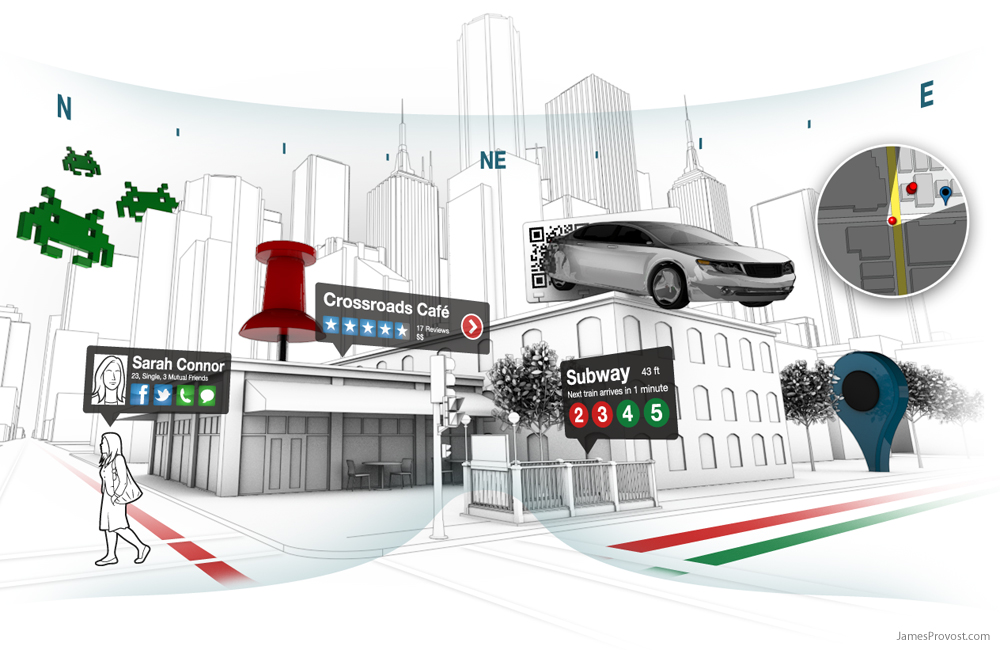
\includegraphics[width=0.80\textwidth]{augmentedVisor.jpg}
  \caption{Representación conceptual de la realidad aumentada (James Provost)}
  \label{fig:augmentedVisor}
\end{figure}

%La realidad aumentada se puede aplicar a prácticamente todos los campos. En el sector industrial, para la reparación y mantenimiento de maquinas e instalaciones complejas, visualización de datos o simulación.  En aplicaciones médicas, mostrarían la situación de órganos no visibles durante una cirugía. También se han realizado aplicaciones para diseño de interiores (IKEA), presentaciones de productos, educación, publicidad, turismo, arte y ocio. 

\begin{figure}[t] 
  \centering
  \includegraphics[width=1.0\textwidth]{RA1.pdf}
  \caption{Jerarquía de la \textit{Realidad Mixta}}
  \label{fig:RA1}
\end{figure}

Según la taxonomía descrita por Milgram y Kishino [16], los entornos de Realidad Mixta son aquellos en los que “se presentan objetos del mundo real y objetos virtuales de forma conjunta en una única pantalla”.

El paradigma general por el cual se mezcla el mundo real y el virtual se denomina \textit{Realidad Mixta}~\cite{kishino1994taxonomy}. En la Figura \ref{fig:RA1} se muestra la jerarquía en la que se clasifica este tipo de paradigma. A la izquierda, se muestra el caso extremo de \textit{integración nula}, en el que la interacción se realiza únicamente a través de los objetos reales. No existe ningún tipo de dispositivo informático con el cual realizar la interacción.

El siguiente paradigma es el de \textit{Realidad Aumentada}. Este paradigma está más cerca del extremo del \textit{entorno real} que del \textit{virtual} porque se parte del \textit{mundo real} como base, y a partir de él se añaden los objetos virtuales. Este paradigma contempla multitud de ventajas y aplicaciones. Henderson y Feiner llevaron a cabo un estudio evaluando las ventajas de la Realidad Aumentada frente a métodos convencionales en tareas específicas como la realización de procesos de mantenimiento~\cite{henderson2009evaluating}. %En el Apartado \ref{cap:ra:aplicaciones} se detallan más aplicaciones de esta tecnología.


Acercándose más hacia el \textit{entorno virtual}, se encuentra el paradigma de la \textit{Virtualidad Aumentada}~\cite{neumann2009modeling}. En un sistema que utilice esta tecnología, se parte de un sistema completamente virtual, que puede ser compartido por varios usuarios, y se interactúa con él a través del mundo real. Algunos proyectos que han utilizado este paradigma se enfocaban como \textit{sistemas colaborativos}, en los que se crean un punto de encuentro virtual (una sala de reuniones, por ejemplo). Algunos de estos proyectos para colaboración son el de Regenbrecht et al. para colaboración~\cite{regenbrecht2004using} y videoconferencia remota~\cite{regenbrecht2003augmented}.

Por último, se encuentran los sistemas de \textit{Realidad Virtual}~\cite{steuer1992defining}, en los que todo es generado por ordenador, y el objetivo es que el usuario se abstraiga lo máximo posible del mundo real, para conseguir una inmersión total en el mundo virtual. Estos sistemas tuvieron un gran auge hace unos años, en su modalidad con \textit{HMD}\footnote{\textit{Head Mounted Display}}, aunque no llegaron a consolidarse completamente. Un proyecto interesante realizado sobre \textit{Realidad Virtual} es \textit{CAVE} de Cruz-Neira et al~\cite{cruz1993surround}. También se realizaron multitud de estudios que probaban la eficacia de este paradigma 




Uno de los principales problemas a resolver es denominado registro. Los objetos del mundo real y virtual deben estar correctamente alineados o la sensación de integración se verá seriamente afectada. Sin un registro preciso, la realidad aumentada no podría ser soportada por muchas aplicaciones, por ejemplo, en medicina para el guiado de una aguja en la realización de una biopsia. 

Las aplicaciones de Realidad Aumentada deben cumplir las siguientes características definidas por Ronald T. Azuma \cite{Azuma}:
\begin{itemize}
\item \textbf{Combinar el mundo real con el virtual.} El resultado final debe mostrar la información sintética sobre las imágenes percibidas del mundo real.
\item \textbf{Debe ser interactivo en tiempo real.} La integración debe ser realizada \emph{en el momento}, por lo que el cálculo necesario debe realizarse n el menor tiempo posible.
\item \textbf{La alineación de los elementos virtuales debe realizarse en 3D.} Los objetos sintéticos deben de estar en el espacio tridimensional.
\end{itemize}

%\subsection{Componentes de un sistema de realidad aumentada}
%Un sistema de realidad aumentada depende de cuatro componentes físicos:

%\begin{itemize}
%\item \textbf{Elementos de entrada y sensores de orientación.} Proporciona al sistema la información visual, la entrada del usuario y, potencialmente, ayudar a la orientación.
%\item \textbf{Fuente de datos.} Proporciona información aplicable al medio ambiente para que el sistema aumente la visión del usuario.
%\item \textbf{Periféricos de retroalimentación de los usuarios.} Principalmente en la forma de producción visual, pero también pueden incluir audio y otras interfaces de usuario.
%\item \textbf{Unidad de procesamiento.} Combina los datos de los sensores de entrada para determinar la orientación y aumentar la visión del usuario con información de la fuente de datos. Envía el resultado a los periféricos de retroalimentación del usuario.
%\end{itemize}

\subsection{Elementos de entrada y sensores de orientación}
Un sistema de realidad aumentada debe ser capaz de conocer su orientación y posición dentro del entorno circundante con el fin de ofrecer una experiencia «aumentada» satisfactoria. La combinación de la orientación y la posición de un observador que se conoce como \emph{pose}. La estimación de la \emph{pose} se definirá con más detalle en la sección 4. La orientación y posición se pueden determinar mediante técnicas de visión por computador, pero hay métodos alternativos para estimar la \emph{pose}  utilizando  sensores diseñados específicamente para medir alguno o todos los parámetros de los seis grados de libertad que componen la \emph{pose}.

\subsubsection{Localización}
La manera más popular para determinar la posición es mediante la utilización del Sistema de Posicionamiento Global (GPS), desarrollado por el ejército de Estados Unidos y totalmente operativo desde 1994. 
Un receptor GPS es lo suficientemente preciso para determinar la ubicación en las aplicaciones de realidad aumentada, además, debido a su bajo coste, los sensores de GPS se llevan incluido en los teléfonos móviles desde 2005.

\subsubsection{Orientación}
En el espacio 3D, la orientación de un cuerpo rígido puede ser determinado de forma única por tres ángulos o grados de libertad (3DOF): \emph{pitch, roll y yaw}. La figura \ref{fig:ángulos}  se puede observar una representación de estos tres ángulos como rotaciones alrededor de sus ejes correspondientes. 

\begin{figure}[b]
  \centering
  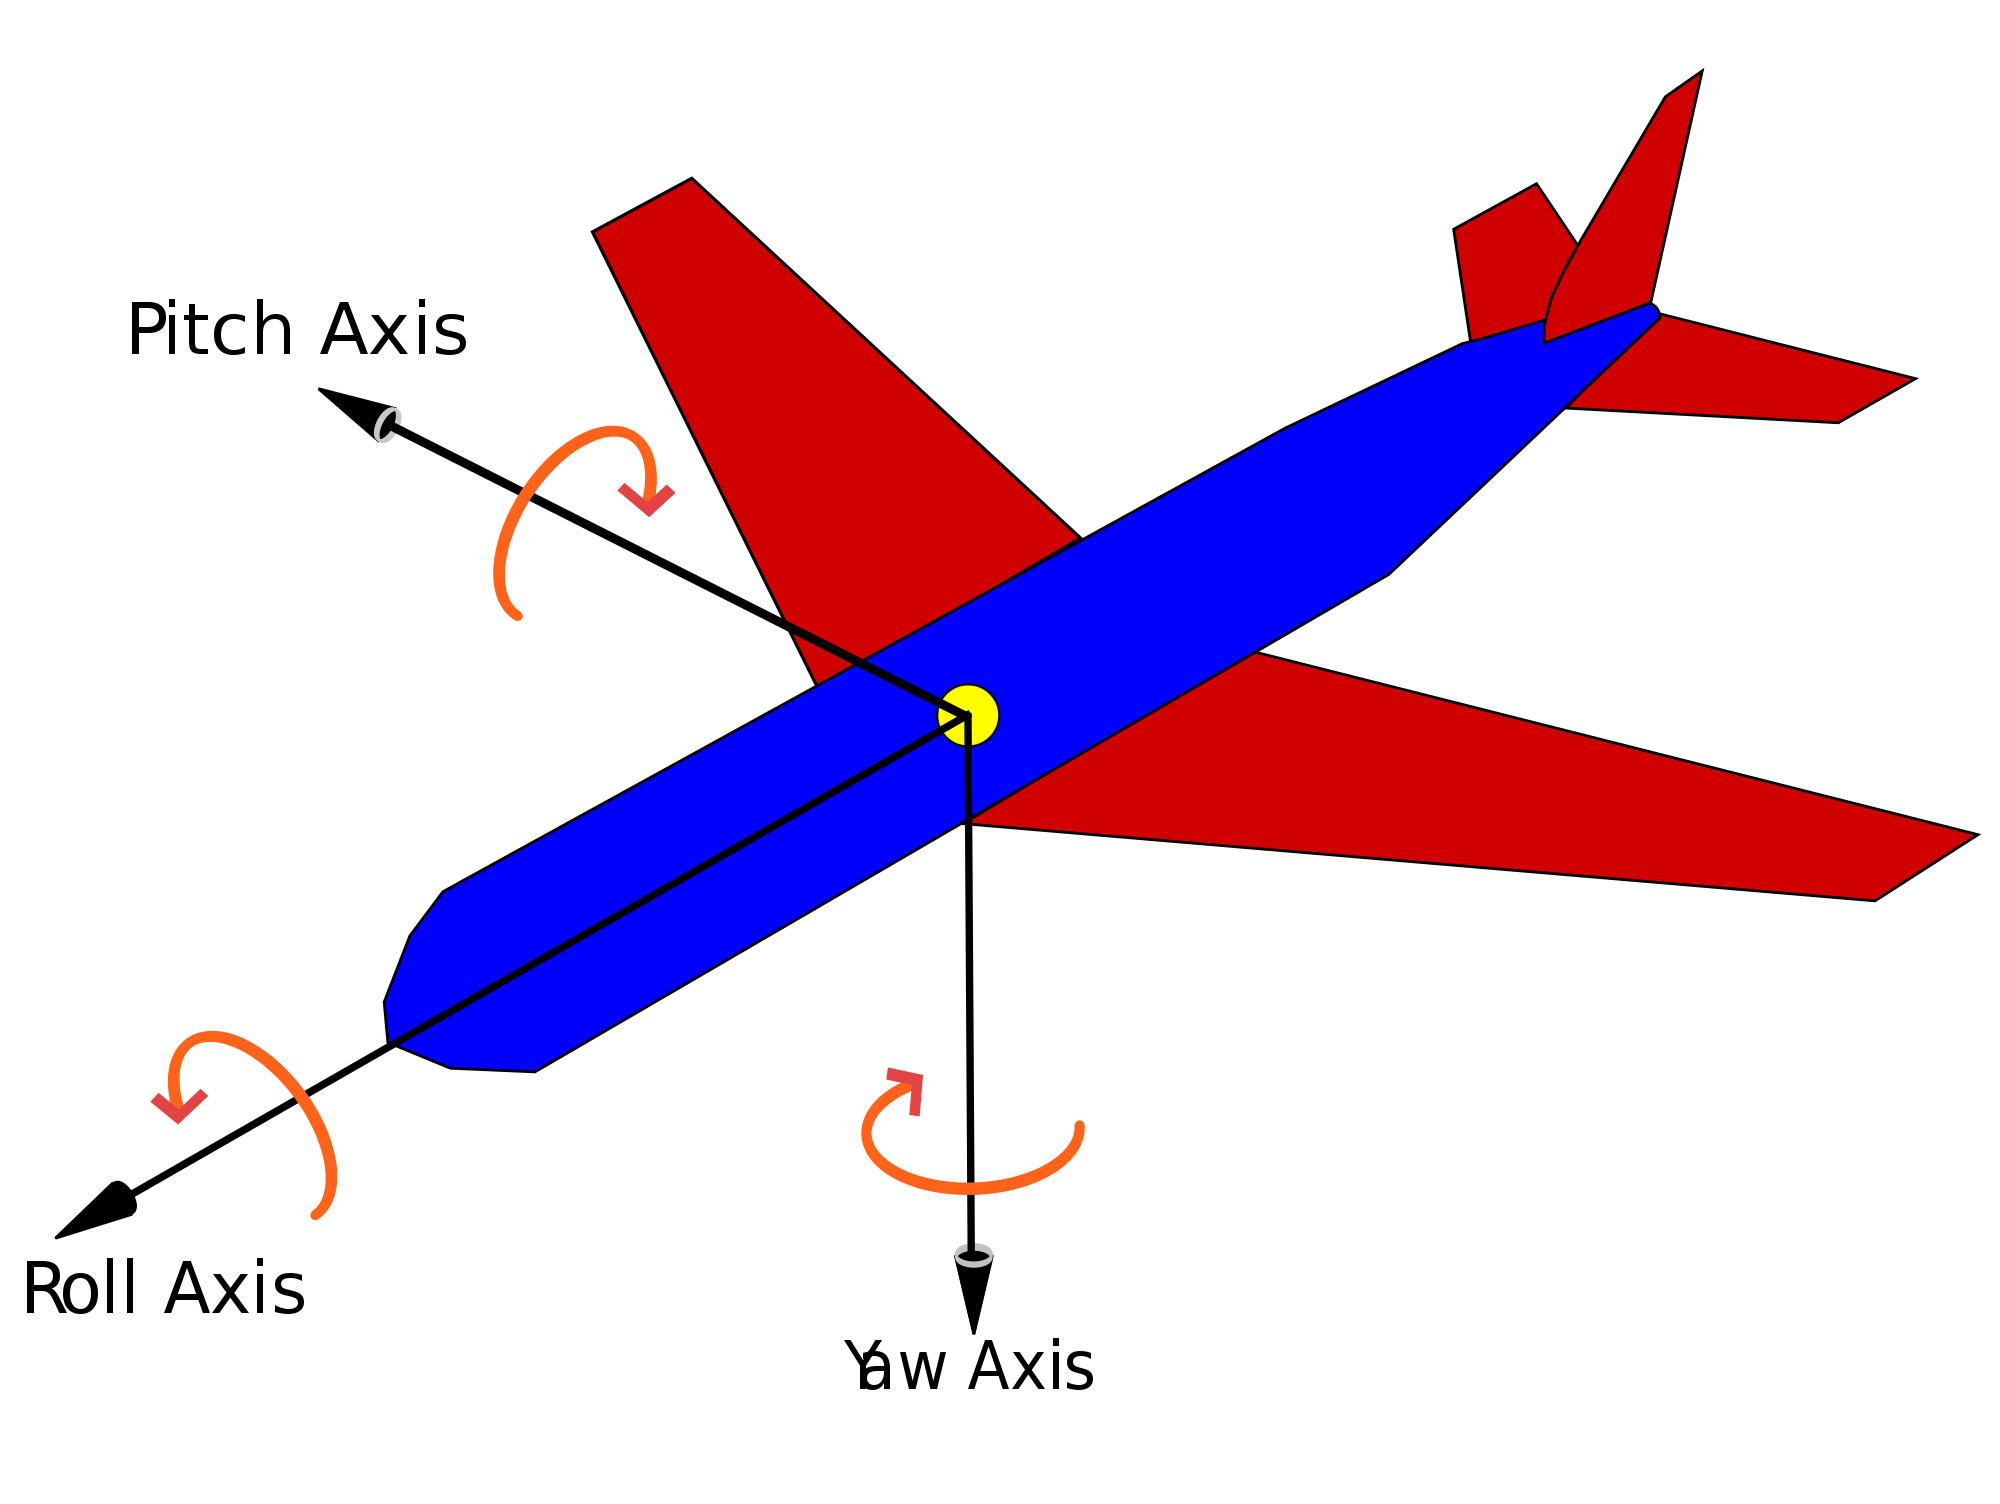
\includegraphics[width=0.5\textwidth]{angles.png}
  \caption{Ángulos de orientación: \emph{yaw, pitch y roll}}
  \label{fig:ángulos}
\end{figure}

Para facilitar la tarea de orientación los dispositivos móviles, sobre todo smartphones y tablets, están equipados una serie de sensores como:

\begin{itemize}
\item\textbf{Sensores magneto-resistivos}, o magnetómetros, que son utilizados como una ``brújula electrónica'' y se utilizan para determinar el \emph{yaw} y la dirección. Las nuevas generaciones de brújulas electrónicas utilizan tres ejes para asegurar una lectura correcta sin importar la inclinación del sensor.
\item\textbf{Acelerómetros} para medir la aceleración aceleración experimentada por un objeto con respecto a un marco de referencia. Los acelerómetros no pueden determinar el \emph{yaw}, pero pueden ser utilizados para determinar el \emph{pitch} y el \emph{roll}. 
\item\textbf{Giroscopios electrónicos} que son utilizados para determinar los tres grados de libertad de orientación a la vez.
\end{itemize}

Un problema común en los sistemas de seguimiento visual es que los movimientos bruscos de la cámara pueden ocasionar que la imagen salga borrosa y verse afectado el seguimiento visual. Un dispositivo híbrido equipado con un giroscopio y un acelerómetro será capaz de determinar rápidamente y con precisión tres de los seis grados de libertad de la \emph{pose} y ayudar al sistema de seguimiento visual a recuperarse cuando se experimentan imágenes borrosas. 

\subsubsection{Fuentes de Vídeo}
La realidad aumentada superpone información sobre lo que el usuario está viendo. Para los sistemas dinámicos en los que la información virtual debe ser mezclada con la imagen real, se requiere un dispositivo de captura, como una cámara digital. Para los propósitos de las aplicaciones de realidad aumentada es preferible una cámara de vídeo. La mayoría de las aplicaciones utilizan una única cámara y se conocen como sistemas monoculares. También existen sistemas estereoscópicos, que  utilizan dos cámaras para determinar la profundidad.

El desarrollo tecnológico en el ámbito de la captura de imagen digital que han mantenido los principales fabricantes en los últimos 10 años, conocido como la «batalla del mega-píxel», ha supuesto un gran avance para disponer de sensores con una gran calidad de imagen y un coste reducido. Actualmente es normal encontrar cámaras de alta resolución en prácticamente todos los dispositivos móviles, permitiendo grabar vídeo en una resolución FullHD ó 4K y obtener imágenes fijas de hasta 7136x5360px.

\subsubsection{Entrada táctil}
En sistemas de realidad aumentada portátiles tales como teléfonos inteligentes o tablets, la pantalla funciona al mismo tiempo como una entrada para manipular objetos directamente en la pantalla y un dispositivo de salida.

\subsection{Fuente de datos}
Un sistema de realidad aumentada requiere una fuente de datos e información con la que aumentar la realidad de un usuario. La fuente de datos puede ser desde una base de datos directamente disponible en el sistema, o puede ser información agregada a partir de fuentes disponibles a través de una conexión de red. Actualmente existe un gran desarrollo para el uso de Internet como fuente de datos para aplicaciones de realidad aumentada. Aplicaciones como Wikitude\footnote{http://www.wikitude.com} y Layar\footnote{http://www.layar.com} son ejemplos de las sistemas que utilizan los datos disponibles en Internet como fuente de datos.

\subsection{Periféricos de retroalimentación de los usuarios}
\subsubsection{Dispositivos  de Visualización}
Existen  muchos métodos y dispositivos para mostrar la información o imágenes generadas para su combinación y alineación con la realidad: 
\begin{itemize}
\item \textbf{Monitores y pantallas tradicionales}
  Sobre todo impulsado por la popularidad de frameworks y bibliotecas como ARToolkit \cite{Kato}, existen muchas implementaciones de realidad aumentada para utilizar con un ordenador de sobremesa o portátil. No requieren de tecnología especial, únicamente una webcam que el usuario puede controlar. La aplicación se suele presentar en una pagina web y permite a los usuarios superponer información o imágenes sobre lo capturado por la webcam. Para la tarea de tracking y registro se utilizan marcadores que el usuario previamente ha impreso.
  
\item \textbf{HMDs (Head Mount Display)} Los HDM o Head Mount Display son dispositivos que permiten al usuario ver el el mundo real con objetos virtuales superpuesto mediante técnicas ópticas y de vídeo. Los HDM se pueden clasificar en dos categorías:
  \begin{itemize}
  \item \textbf{Ópticos (OST - Optical See-Throug)} Permiten al usuario ver el mundo real a través de sus ojos y la imagen virtual se muestra mediante elementos ópticos holográficos, espejos semi-plateados o alguna otra técnica similar. Un ejemplo de este tipo de dispositivo son las Google Glass.
    
  \item \textbf{Vídeo (VST - Vídeo See-Throug)} En los dispositivos de esta categoría, el usuario percibe tanto el mundo real como la imagen virtual mediante una o varias pantallas. Como ventajas de los VST esta una mayor consistencia entre el mundo real y el virtual.
  \end{itemize}
  
\item \textbf{Visualización basada en proyección}
  Un sistema de visualización basado en proyección es una buena opción para sistemas fijos, además proporciona una intrusión mínima y la capacidad de interacción con varios usuarios.
  Se han propuesto una gran variedad de técnicas de visualización mediante proyectores sobre objetos y otras superficies (no necesariamente pantallas). Ehnes \cite{Ehnes} amplió el trabajo anterior de Pinhanez \cite{Pinhanez} sobre la proyección de vídeo para mostrar imágenes virtuales sobre objetos reales directamente utilizando técnicas de tracking de vídeo para seguir el movimiento y manteniendo la imagen sobre objeto mientras este se mueve.
  
\item \textbf{Dispositivos portátiles (smartphones, tablets)}
  Hoy en día el dispositivo portátil por excelencia es el smartphone. Es mínimamente invasivo, muy portable y ampliamente extendido. Según el informe de comScore \footnote{http://www.comscore.com/esl/Insights/Presentations-and-Whitepapers/2013/2013-Spain-Digital-Future-in-Focus} el 66\% de los españoles tienen un teléfono inteligente, por lo que son una gran alternativa para la visualización de aplicaciones de realidad aumentada.
\end{itemize}

\subsubsection{Audio}
El audio se utiliza principalmente de dos formas diferentes en los sistemas de realidad aumentada: como una modalidad de la interfaz de usuario multimodal o para ofrecer una experiencia aural aumentada. 

Por ejemplo, el usuario pueda ser capaz de dar comandos de voz y el sistema devuelva retroalimentación con señales de audio (pitidos). Este tipo de audio no direccional es trivial desde el punto de vista tecnológico aportando una nueva dimensión a las aplicaciones móviles. El audio aumentado puede servir a personas con discapacidad visual para ayudar a comprender el entorno. Mediante unos altavoces o un par de auriculares, es bastante simple proporcionar al usuario la información en forma de audio. La síntesis de voz también se puede utilizar para leer información, por ejemplo, leer palabras en voz alta desde un sistema de reconocimiento de texto.

\subsection{Unidad de procesamiento}
%\subsubsection{Dispositivos móviles: Smartphones,  tablets y SBCs (Single Board Computer)}
El teléfono móvil ha evolucionado hacia una plataforma informática móvil (smartphone), en la que desarrollar las actividades habituales de un ordenador personal. El principal inconveniente de estos era la pantalla reducida que disponen lo que ha derivado en el desarrollo de un nuevo dispositivo denominado tablet. 

Las tablets disponen de prácticamente las mismas características que los smartphones (incluso el mismo sistema operativo) pero las pantallas son mayores, sin necesidad de teclado físico ni ratón, con las que se interactúa principalmente mediante la pantalla táctil con los dedos o un stylus.

Otra tendencia tecnológica es el desarrollo de SBCs, \textit{(Single Board Computer)} que básicamente es un ordenador completo montado sobre un circuito. Su diseño se basa en un microprocesador de bajo rendimiento (normalmente de arquitectura ARM), RAM y diversos dispositivos de E/S como puertos USB, lectores de tarjetas, conectores Ethernet, y salida de audio y vídeo con un precio final muy reducido. Este tipo de dispositivos se crearon para utilizarlos con fines educativos, pero entre la comunidad de usuarios, debido a su gran versatilidad se utilizan para múltiples aplicaciones tales como centros multimedia o distintos tipos de servidores dado su bajo consumo.  

\section{Técnicas de Visión por Computador}
En esta sección comentaremos las técnicas que pueden utilizarse para el tratamiento previo de imágenes que se utilizarán para la detección y tracking en sistemas de realidad aumentada. El orden en que se introducen suele ser el aplicado  habitualmente.

La adquisición de imágenes es el primer paso en un sistema de realidad aumentada y es dependiente de la plataforma del sistema. Por norma general, se considera que las imágenes se adquieren con 24 bits, un canal por cada una de sus componentes de color en 8 bits: rojo, verde y azul. También vamos a asumir que las imágenes se adquieren a 30 fotogramas por segundo. Esta suposición esta basada en la transmisión típica con la que trabajan la mayoría de webcams.

\subsection{Preprocesado de las imágenes de entrada}
Prácticamente todas las técnicas presentadas procesan y trabajan las imágenes en blanco y negro. Aún realizando la captura en color, normalmente se realizan varios pasos previos para reducir y simplificar la cantidad de información que se tiene que manejar, dejando solo la información esencial.

Por ejemplo, un frame típico obtenido a partir de una webcam o la cámara de un teléfono móvil puede tener una anchura de 640 píxeles y 480 píxeles de altura. Suponiendo que una imagen en color con tres canales (rojo, verde y azul) se obtiene con ocho bits por canal, la cantidad de datos por frame serian 640 x 480 x 3 x 8 = 7.372.800 bits de información. Esto es para una sola imagen. La mayoría de cámaras tienen una tasa de transferencia entre 20 y 30 frames por segundo, lo que significa que para cada frame se debe procesar toda esa información por completo cada 33 milisegundos antes de que llegue el siguiente fotograma. Sería muy costoso (e innecesario), por lo que se utilizan una serie de técnicas como las explicadas a continuación para reducir la cantidad de información requerida en las etapas posteriores.

\subsubsection{Conversión a escala de grises}
La reducción del número de canales de la imagen (rojo, verde y azul) a un solo canal de ocho bits representados como gris, reduce la cantidad de datos a procesar en un factor de tres. Una imagen en escala de grises representa la intensidad de la imagen. 

No existe un único método para convertir una imagen en color a escala de grises, el proceso más común consiste en recorrer todos los píxeles de la imagen, y para cada píxel de forma individual multiplicar sus componente RGB (rojo, verde y azul), cuyos valores oscilan entre 0 y 255, por unos coeficientes y sumarlos. De esta forma obtenemos la misma luminosidad del píxel tanto en color como en escala de grises.

Los componentes RGB originales del píxel se sustituyen por el valor resultante de esa suma. Los tres componentes con el mismo valor, para lograr así el efecto de escala de grises, ya que cuando los tres componentes tienen un mismo valor lo que se obtiene es un tono gris, excepto en los extremos, donde (0, 0, 0) es negro y (255, 255, 255) es blanco.

Los coeficientes que se utilizan son 0.299 para el rojo (R), 0.587 para el verde (G), y 0.114 para el azul (B). Al sumar los tres coeficientes el total vale 1 (0.299 + 0.587 + 0.114), lo que garantiza que el valor resultante de la suma de los productos por los componentes originales del píxel será un valor comprendido también entre 0 y 255.

\subsubsection{Thresholding (umbralización o binarización)}
La umbralización consiste en definir un valor umbral y compararlo con cada uno de los píxeles de la imagen. A los píxeles que estén por debajo del umbral se les asigna un valor, y a los que estén por encima otro. De esta forma se divide toda la población de valores en tan sólo dos grupos, reduciendo considerablemente la complejidad de la información a analizar.

Aplicar un valor umbral a una imagen presenta dos dificultades. La primera es decidir que valor concreto tomar, y la segunda es conseguir que dicho valor sirva para cualquier imagen posible que pueda llegar desde la webcam. Si los píxeles tienen un valor que se encuentra dentro del rango que va de 0 a 255, ¿cúal es el mejor valor para el umbral? ¿128, que está en la mitad del rango? ¿Y por qué no 57? No se puede decidir de antemano sin analizar antes la imagen, ya que el mayor inconveniente que presenta este procedimiento es que es muy sensible a la iluminación. Con poca iluminación los píxeles tienden a tomar valores bajos, oscuros, cercanos al 0, y con mucha iluminación toman valores altos, claros, cercanos al 255. Y peor es el caso cuando la iluminación varía dentro de la propia imagen, con algunas zonas muy oscuras y otras muy claras.

El algoritmo de umbralización adaptativa, no aplica el umbral de una manera global sobre todos los píxeles de la imagen, sino que tiene en cuenta las variaciones en la iluminación de una manera local para cada píxel de forma individual. Algo que consigue tomando el valor original de cada píxel de la imagen en escala de grises, y comparándolo con otro valor calculado que sea algún tipo de media de los valores de los píxeles que tiene alrededor. En las zonas homogéneas el valor del píxel se asemejará mucho a la de la media de sus vecinos, mientras que en las zonas de transición abruptas, en los bordes, se diferenciará de dicha media.

La función utiliza un filtro gaussiano para calcular los valores medios de los píxeles. La aplicación de un filtro sobre una imagen normalmente consiste en recorrer todos los píxeles de la imagen, y para cada píxel de forma individual aplicar una operación que genere un nuevo valor para el píxel. En nuestro caso, para conseguir difuminar la imagen de forma coherente, se utiliza como base para calcular el nuevo valor para cada píxel, los píxeles más cercanos que tiene a su alrededor. Es decir, si tenemos un píxel negro rodeado de píxeles blancos, lo que se quiere obtener es un nuevo píxel gris que difumine la imagen, eliminando ese \textit{ruido} que representa el píxel negro aislado.

El proceso consiste es definir un tamaño de ventana o kernel, por ejemplo de 3x3 píxeles, a cada celda de este kernel asignarle un coeficiente numérico, y mover el kernel por encima de cada píxel de la imagen original de forma individual, multiplicando los coeficientes del kernel por los valores de los píxeles que cubre cada una de las celdas.

Unos mejores coeficientes serían aquellos que dieran más importancia al píxel original, y fueran decrementado la importancia a medida que se fueran alejando de él. Y eso es precisamente lo que persigue el filtro gaussiano, lo que consigue usando unos coeficientes que se calculan con la siguiente fórmula:

\begin{equation}
  \frac{1}{2 \cdot \pi \cdot \sigma^{2}} \cdot e^{\frac{-(x^2 + y^2)}{2 \cdot \sigma^{2}}}
\end{equation}

Donde $x$ e $y$ son la distancia al píxel original, y $\sigma$ (sigma) la desviación típica de la distribución gaussiana. 

De igual forma que en el proceso de conversión a escala de grises, se verifica que la suma de los coeficientes es igual a 1, y como se observa, los coeficientes centrales tienen mucho más peso que los de los extremos. Aunque sólo se ha indicado una fila, en la práctica ha de verse como una matriz de 7x7 con los coeficientes distribuidos de manera uniforme alrededor del elemento central. 

Implementar el filtro resulta sencillo, pero muy lento, ya que por cada píxel hay que realizar 49 (7x7) multiplicaciones. No obstante, el filtro tiene una característica particular. Es un filtro "separable", lo que quiere decir que se puede aplicar en un primer paso en horizontal, multiplicando cada píxel sólo por la fila central del kernel, y al resultado de ese primer paso aplicarle el filtro en vertical, multiplicando cada píxel nuevamente sólo por la fila central. De esta forma se reduce a 14 (7x2) multiplicaciones por píxel. 

Este filtro plantea un problema de implementación en los bordes, donde el kernel abarca píxeles que no existen, y que se ha resuelto duplicando los píxeles de los bordes para cubrir el kernel. Aunque existen otras estrategias posibles.

A los píxeles que están por debajo del umbral se les asigna un 1, y a los que están por encima un 0. De esta forma se obtiene una imagen "binaria", en el sentido de que sólo tiene dos valores (blanco y negro).

\subsubsection{Corrección de perspectiva y proyección}
La captura de documentos mediante cámaras normalmente se realiza sin estar la cámara paralela al plano en el que se encuentra, con lo que obtendrá una imagen con una distorsión de la perspectiva. 
Si los detectores son tolerantes a la perspectiva no es necesaria una rectificación. Sin embargo, la mayoría de procesadores de OCR son muy sensibles a la variaciones del texto bajo perspectiva y fallan.

Si la deformación de la perspectiva producida es ligera, la rectificación se puede realizar por aproximación \cite{Hsieh}. En general, supongamos que el documento está en un plano; entonces la transformación proyectiva del plano del documento en el plano de imagen puede ser modelado por una matriz de 3 x 3 en el que ocho coeficientes son desconocidos y uno es el factor de normalización. La eliminación de la perspectiva se puede realizar una vez que se encuentran los ocho incógnitas. Con cuatro pares de puntos correspondientes son suficientes para recuperar los ocho grados de libertad. Bajo el supuesto de que los bloques de texto son rectángulos en un mundo 3D, Jung \cite{Jung}  utiliza un enfoque directo para establecer cuatro pares de correspondencias y proceder a la rectificación. Sin embargo, este método es muy propenso a errores y por lo tanto sólo puede utilizarse cuando la deformación de la perspectiva es pequeña.

En otros casos, el texto aparecerá sobre superficies curvas, como en los casos de que estemos capturando las páginas de un libro abierto. Estos casos típicos permiten que se realicen suposiciones, como la de utilizar un modelo cilíndrico de para calcular la deformación \cite{Kanungo}. Del mismo modo, si suponemos que el texto aparece como líneas rectas paralelas en la página, podemos utilizar la línea de texto para calcular la deformación que se esta produciendo en la página y obtener la imagen como si estuviese sobre un plano.

\subsubsection{Downsampling}
Otra técnica que se utiliza es la de \emph{downsampling} para reducir el número total de píxeles de la imagen. Lo ideal sería que la relación de aspecto de la imagen original se conserve siempre, para ello el número de píxeles se reduce a la mitad en cada iteración. Cada \emph{downsampling} que se realice sobre una imagen lleva como consecuencia la pérdida de datos que reducirá la precisión del tracking y podría influir en la robustez. A la hora de diseñar el sistema se debe decidir si es aceptable una pequeña pérdida de precisión o emplear un enfoque multiresolución, en el que se realiza el tracking completo por primera vez en una imagen reducida y los resultados se refinan con versiones de mayor resolución de la imagen \cite{Klein}.

La teoría sobre los diferentes niveles de resolución está presentado por Adelson \cite{Adelson} y se describe como un conjunto de copias (con filtros paso bajo o paso banda de una imagen), donde cada una de ellas es una representación de la imagen en una escala diferente. Son esencialmente representaciones a escala múltiple de una imagen a partir de la imagen original y con una escala de un factor de dos en cada paso hacia abajo. Este proceso puede ser visualizado como una pirámide con la imagen original en la parte inferior. 

\begin{figure}
  \centering
  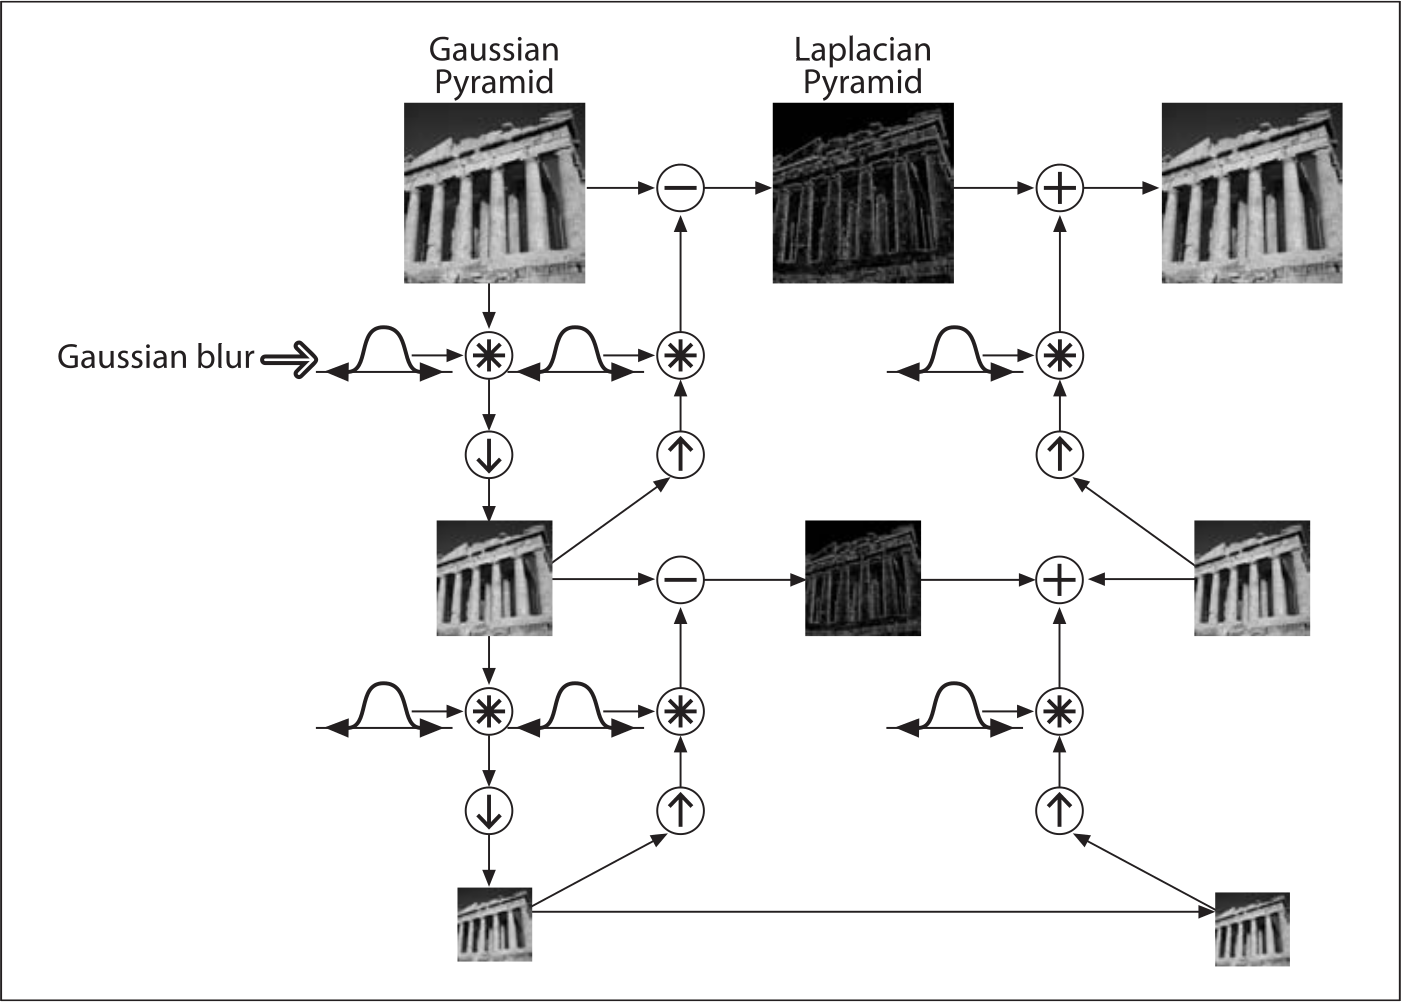
\includegraphics[width=0.8\textwidth]{downsampling.png}
  \caption{Cálculo de las pirámides de Gauss y sus inversas (Laplace). (Bradski y Kaehler)}

  \label{fig:pirámides}
\end{figure}

La figura \ref{fig:pirámides} muestra los pasos involucrados en el cálculo de una pirámide de imágenes y la pirámide laplaciana, que contiene toda la información perdida en cada paso. Si la pirámide de la imagen y la pirámide laplaciana están disponibles, la imagen original puede ser perfectamente reconstruida. En cada nivel de la pirámide, la imagen contiene cuatro veces menos píxeles que la capa inferior (Figura \ref{fig:pirescale}) lo que afectará directamente al tiempo total de procesamiento. 

\begin{figure}
  \centering
  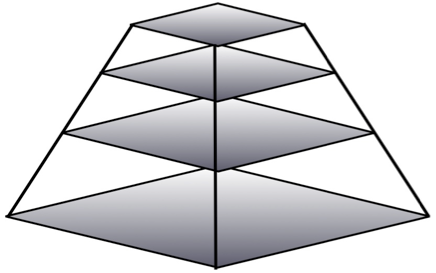
\includegraphics[width=0.5\textwidth]{pyramid.png}
  \caption{Pirámide multiresolución. (journal.code4lib.org)}
  \label{fig:pirescale}
\end{figure}

\section{Detección}
En el contexto de la realidad aumentada, la detección es el proceso de localizar un objeto en una imagen capturada y calcular la posición y orientación de la cámara \emph{(camera pose)} respecto a ese objeto.

Los enfoques que se han dado en las distintas técnicas de detección se pueden clasificar en dos tipos: La detección mediante marcas de referencia o mediante puntos de interés naturales.

\subsection{Detección basada en marcas de referencia \emph{(fiducial markers)}}
Una marca de referencia es un objeto que se coloca en el campo de visión de la imagen a procesar y proporciona un punto de referencia y unas dimensiones conocidas de antemano, facilitando el proceso de detección y el calculo de la pose.

Mediante este método Kato presentó en 1999 un paper que utilizaba marcas cuadradas con un borde negro para calcular la pose de la cámara en tiempo real\cite{Kato}. El resultado fue la biblioteca ARToolKit que ha popularizado la realidad aumentada.

Otros papers en la misma línea, como el de Stricker \cite{Stricker}, en el que describe un método para encontrar las coordenadas 3D de las 4 esquinas de un marcador cuadrado, mientras que Park \cite{Park2} describe un algoritmo para el cálculo de la pose de la cámara a partir de características conocidas.

Hasta el año 2002, las técnicas mediante marcas se habían estudiado ampliamente. Zhang \cite{Zhang} realizo un estudio recopilando y comparando varios de los principales enfoques que existían. A partir de esta fecha no se han presentado nuevos sistemas basados en marcadores.

\subsection{Detección basada en puntos de interés naturales}

El aspecto más importante de la detección de puntos de interés es hacerlo lo más coherente posible. Los mismos puntos de interés que se detectan en un frame, debe detectarse de nuevo en el siguiente cuadro, dado que todavía siguen presentes en la imagen. 

Si tenemos un rectángulo sin bordes en movimiento delante de un fondo del mismo color, sería imposible de rastrear porque el sistema no podría distinguir dos puntos distintos en la imagen. Si tenemos un punto negro sobre un fondo blanco, y esté empieza a moverse, es muy fácil de seguir, ya que el sistema sólo tendría que encontrar ese punto en los siguientes frames. Este punto puede ser visto como una discontinuidad o un punto en el que se produce un cambio busco en la intensidad de la imagen.

Por tanto, el requisito deseable para considerar a un punto de interés es que debe ser una discontinuidad. Si tuviéramos muchos más de estos puntos también sería imposible diferenciar entre ellos y tendríamos el mismo problema que con el rectángulo del mismo color del fondo. Sólo podremos distinguirlos si la región que rodee al punto de interés es diferente, al menos en cierto grado, de la región local que rodea a todos los demás. Por tanto, el segundo requisito de un punto de interés es que él y la región que lo rodea debe ser único. 

Prácticamente en todos los trabajos sobre detección mediante puntos de interés se pueden establecer las siguientes fases:

\begin{description}
\item[Extracción] El proceso de extracción consiste en la búsqueda de zonas en la imagen con diferente apariencia que las que están a su alrededor, denominadas características \emph{(features)}. Normalmente las características suelen ser bordes, esquinas o zonas mas brillantes u oscuras en función del algoritmo utilizado en particular. A esta fase también se la denomina detección.

  Existen muchos algoritmos de detección, que obtienen distintas tipos de características, por ejemplo, el detector de esquinas de Harris\cite{Harris} o el algoritmo FAST \cite{Rosten} que devuelve los píxeles con valores máximos y mínimos en función de sus vecinos mediante técnicas de Machine Learning.

\item[Descripción] Se calcula el vector que describe la característica de un punto significativo para la posterior comparación entre otros puntos de interés. Los enfoques basados en el uso de descripción locales han sido ampliamente investigados y se dividen en dos tipos: el histograma de gradientes y la prueba binaria.

  El histograma de gradientes se calcula a partir de la cuantificación de los gradientes dentro de una área local. En SIFT \cite{Lowe}, una zona se divide en subregiones y se calcula el histograma de gradiente en cada una de ellas. Este enfoque es utilizado y mejorado en los trabajos de Ambai \cite{Ambai}, Bay (SURF) \cite{Bay}, y Wagner \cite{Wagner}

  Una prueba binaria es una comparación de la intensidad de dos píxeles y produce un resultado binario que representa qué píxel es más brillante. Se realizan cientos de pruebas para calcular un vector de características, ya que solo una de ellas no es lo suficientemente discriminatoria. El tema de investigación principal de este enfoque es el de muestreo eficiente entre dos píxeles y es utilizado en los métodos BRIEF \cite{Calonder}, BRISK \cite{Leutenegger}, y ORB \cite{Rublee}. 

\item[Búsqueda de Coincidencias] Los vectores de características se almacenan en una base de datos. Cuando se busca una coincidencia, se accede a la base datos con los datos del vector de consulta y se devuelve el vector almacenado mas similar.

  Si un vector de características es de grandes dimensiones como en SIFT \cite{Lowe}, la búsqueda completa no se podría realizar para tareas en tiempo real. En lugar de ello,  se utilizan técnicas de árboles de búsqueda basado en la aproximación al vecino más cercano \cite{Arya} \cite{Muja}. El costo de la búsqueda de este enfoque depende del número de características almacenados en la base de datos. Otro tipo de búsqueda consiste en mapear el vector de características a un índice de tipo entero \cite{Datar} y almacenarlo en una tabla hash. Este enfoque es teóricamente rápido con $O(1)$, independientemente del tamaño de la base de datos, pero es sensible a errores. Si un vector de características se describe como cadena binaria, se realizará una búsqueda completa en toda la tabla \cite{Calonder}. Para intentar corregir esto, se han planteado la utilización de árboles aleatorios \cite{Lepetit} y estructuras no jerárquicas \cite{Ozuysal}.
\end{description}

Hay muchas clases de detectores de características, pero los más utilizados son los detectores de esquinas (\emph{corners}), de bordes (\emph{edges}) y de regiones (\emph{blobs}). 

\subsubsection{Detector de esquinas de Harris}
El ejemplo más obvio de un punto de interés es una esquina, o la intersección de dos bordes. A lo largo de los años se han desarrollado una serie de algoritmos de detección de esquinas. La mayoría de los algoritmos de detección de puntos de interés calculan una función $C$ de respuesta, ya sea para todos los píxeles, o sólo algunos píxeles seleccionados. 

Probablemente el más famoso detector de esquinas se conoce como ``detector de esquinas de Harris'' desarrollado por Harris \cite{Harris}, que fue creado para la interpretación 3D de secuencias de imágenes. Al igual que con el detector de bordes de Canny, el cálculo de la segunda derivada parcial de una imagen en una dirección específica indicará regiones con cambios bruscos de intensidad de la imagen (discontinuidades) en esa dirección. Dada una imagen en escala de grises en dos dimensiones, $I$, de modo que la intensidad de la imagen en un píxel específico se da por $I(x,y)$, Harris determina $C_{Harris}$ para un punto específico de la siguiente manera: 

En primer lugar, tomamos una región de la imagen encima del área $(u,v)$ y cambiándolo por $(x,y)$. La forma de la región puede ser circular o rectangular. La suma ponderada de las diferencias de los cuadrados (SSD) entre estas dos regiones ,denotada por $S$ y viene dada por:
\begin{equation}
  S(x,y) = \sum_u \sum_v w(u,v) \, \left( I(u+x,v+y) - I(u,v)\right)^2
\end{equation}

$I(u + x, v + y)$ puede aproximarse por una serie de Taylor. Donde $I_x$ y $I_y$ son los gradientes vertical y horizontal de la imagen (derivadas parciales de $I$), tenemos:

\begin{equation}
  I(u+x,v+y) \approx I(u,v) + I_x(u,v)x+I_y(u,v)y
\end{equation}

Esto produce la aproximación:
\begin{equation}
  S(x,y) \approx \sum_u \sum_v w(u,v) \, \left( I_x(u,v)x + I_y(u,v)y \right)^2,
\end{equation}

que se puede escribir en la forma de matriz:
\begin{equation}
  S(x,y) \approx \begin{pmatrix} x & y \end{pmatrix} \textbf{H}_{harris} \begin{pmatrix} x \\ y \end{pmatrix},
\end{equation}

donde  $\textbf{H}_{harris}$ es la \emph{structure tensor},
\begin{equation}
  \textbf{H}_{harris} = \sum_u \sum_v w(u,v) 
  \begin{bmatrix}
    I_x^2 & I_x I_y \\
    I_x I_y & I_y^2 
  \end{bmatrix}
  =
  \begin{bmatrix}
    \langle I_x^2 \rangle & \langle I_x I_y \rangle\\
    \langle I_x I_y \rangle & \langle I_y^2 \rangle
  \end{bmatrix}
\end{equation}

$\textbf{H}_{harris}$ is conocida como la \emph{Matriz de Harris}. Un punto de interés se caracteriza por una variación de $S$ en todas la direcciones del vector $(x,y)$. Si definimos $\lambda_1$ y $\lambda_2$  como los autovalores de la matriz descrita arriba, podemos definir entonces la función de autocorrelación $C_{harris}$  como:

\begin{equation}
  C_{harris} = \lambda_1 \lambda_2 - \kappa \, (\lambda_1 + \lambda_2)^2 = \operatorname{det}(\textbf{H}_{harris}) - \kappa \, \operatorname{trace}^2(\textbf{H}_{harris})
\end{equation}

En función de los autovalores de $\textbf{H}_{harris}$, $\lambda_1$ y $\lambda_2$, podremos distinguir los siguientes casos:
\begin{itemize} 
\item La función tendrá un máximo si ambos autovalores son altos, lo que quiere decir que un desplazamiento en cualquier dirección  va a producir un incremento importante, indicando, por tanto, que se trata de una esquina.

\item La función sera casi nula si ambos autovalores son bajos, es decir que un desplazamiento en cualquier dirección va a producir cambios muy pequeños, por tanto, la región que engloba la subventana es de intensidad constante (pertenece al mismo objeto).

\item Si un autovalor es alto y el otro bajo, entonces, la función tendrá forma de cresta. Por tanto, sólo los desplazamientos en una dirección van a producir pequeños cambios en C(x,y) y cambios significativos en la dirección perpendicular. Esto indicará la presencia de un borde.
\end{itemize}

El valor de $\kappa$ es un parámetro experimental y es determinado empíricamente del rango de 0.04 a 0.15.

\subsubsection{Shi-Tomasi} 
Shi y Tomasi \cite{ShiTomasi} mejoraron el detector de Harris y encontraron que se obtenía un buen resultado en la detección de esquinas, siempre y cuando el autovalor más pequeño era mayor que un cierto umbral. $C_{ShiTomasi} = min(\lambda_{1}, \lambda_{2})$. La función $C_{ShiTomasi}$ tiene el inconveniente de necesitar el cálculo explícito de los autovalores, que costoso computacionalmente. Los autovalores de una matriz de 2x2 se calculan de la siguiente forma: 

\begin{equation}
  \lambda_{12} = \dfrac{1}{2}(trace(\textbf{H}_{harris}) \pm \sqrt{\operatorname{trace}^{2}(\textbf{H}_{harris}) - 4 \operatorname{det}(\textbf{H}_{harris})})
\end{equation}

El cálculo de la raíz cuadrada puede afectar negativamente el tiempo de cálculo. Los resultados muestran que Shi-Tomasi tiene mejor criterio para determinar a un punto de interés, devolviendo más puntos que Harris para un mismo umbral. Los resultados también muestran que Shi-Tomasi es más lento que el algoritmo de Harris para el mismo umbral, posiblemente debido al cálculo de los autovalores. 

\subsubsection{FAST (Features from Accelerated Segment Test)} 
FAST es algoritmo de detección de esquinas presentado por Rosten y Drummond \cite{Rosten}. En contraste con los métodos de detección de puntos de interés, como Harris, FAST tiene un enfoque mucho más cualitativo, y mucho menos costoso, para determinar si un píxel representa una esquina. Para cada píxel, $p$, en una imagen en escala de grises, FAST examina 16 píxeles en un círculo de radio 3 alrededor de $p$, como se muestra en la figura \ref{fig:fast}. La intensidad (valor de gris) de un píxel está dado por $I(x, y)$. FAST simplemente afirma que $p$ puede ser clasificado como un punto de interés si las intensidades de al menos 12 puntos contiguos en el círculo de prueba son más claros o más oscuros que $I(x_p, y_p)$ (la intensidad de p) para un cierto  umbral, $t$. Un punto de interés puede ser categorizado como ``positivo'' (brillante) si por lo menos 12 puntos circulares contiguos tienen intensidades mayores que $I(x_p, y_p) + t$, o ``negativo'' (oscuro) si sus intensidades son más pequeños que $I(x_p , y_p) - t$. Esta partición puede ser útil para que los puntos positivos no sean comparado con puntos negativos en etapas posteriores del tracking.

\begin{figure}
  \centering
  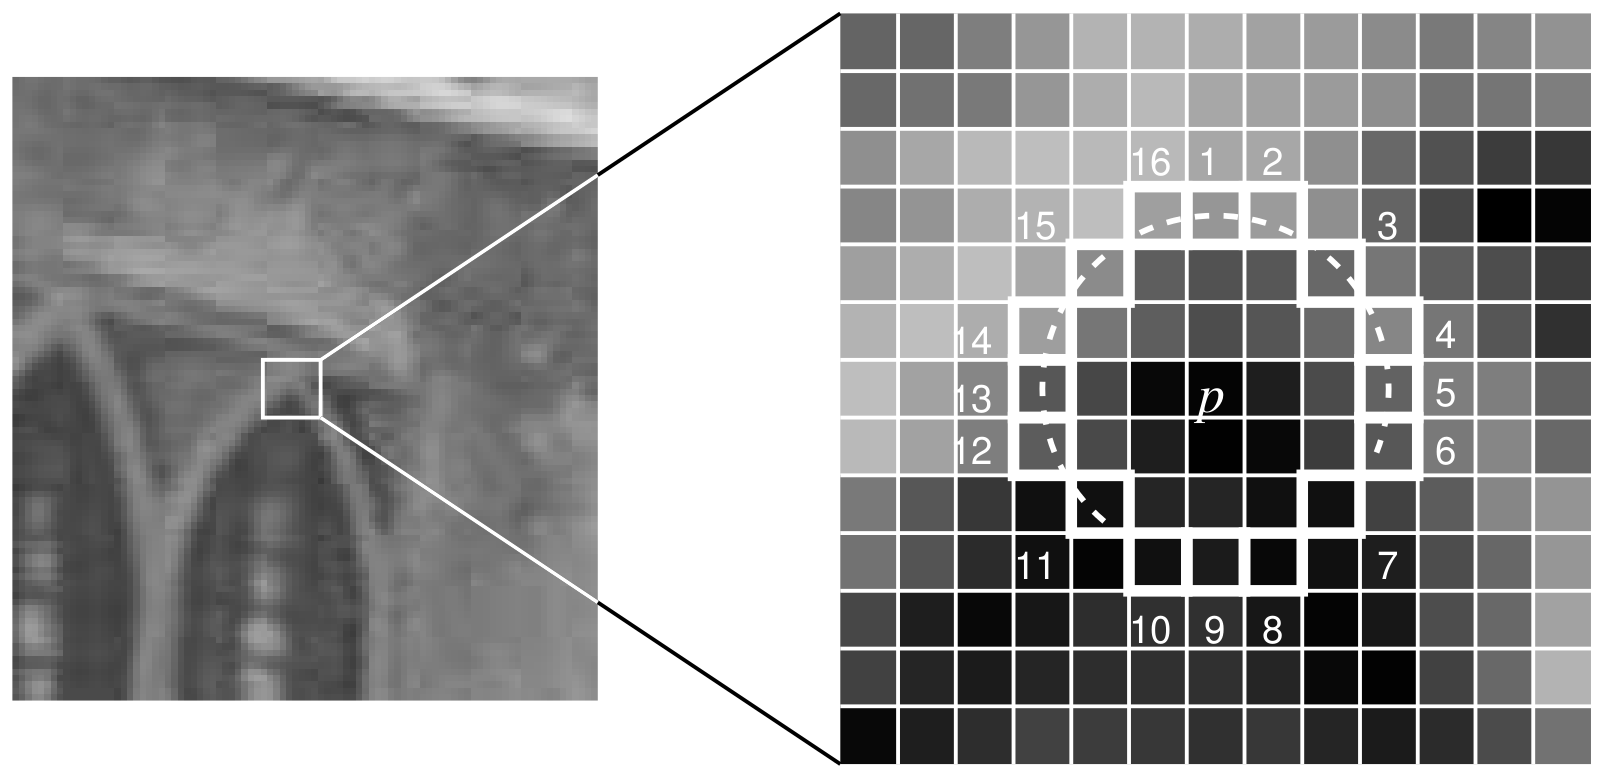
\includegraphics[width=0.8\textwidth]{fast.png}
  \caption{FAST: Círculo de análisis alrededor del píxel $p$. (Rosten y Drummond)
  }
  \label{fig:fast}
\end{figure}

Dado que los 12 puntos deben ser contiguos, la comprobación puede ser acelerada examinando inicialmente soló los píxeles 1, 9, 5 y 13. Un punto de interés sólo puede existir si tres de estos puntos de prueba son todos más brillante o más oscuro que la intensidad de $p$ dado un valor para el umbral. Si más de uno de estos puntos de prueba está  dentro del rango del umbral, $p$ puede ser rechazado de inmediato. Si esta comprobación inicial es satisfactoria, se comprueban el resto de píxeles que quedan en el círculo. Rosten encontró que debido a esta optimización, el algoritmo examina en promedio sólo 3,8 píxeles del círculo para probar si un punto dado es un punto de interés.

De la descripción del algoritmo FAST se puede observar dos potenciales ventajas sobre otros detectores de puntos de interés:
\begin{description}
\item[Rapidez.] Todo lo necesario para procesar una imagen completa es un promedio de 3,8 sumas enteras y comparaciones por píxel. En comparación con otros detectores que requieren el cálculo de derivadas parciales, raíces cuadradas y circunvoluciones, FAST es mucho menos complejo computacionalmente.
\item[Umbralización simple.] El valor del umbral, $t$, es un valor entero que oscila entre 0 y 255 para una imagen en escala de grises de 8 bits. La elección de $t$ influirá directamente en el número, y, posiblemente en la calidad de los puntos de interés detectados. Para aplicaciones en las que es necesario tener un número constante de puntos de interés que deban ser detectados, $t$ puede ser determinado dinámicamente.
\end{description}

Se debe tener en cuenta que estas características conllevan una serie de desventajas en el uso de FAST: 
\begin{enumerate}
\item FAST funciona mal en imágenes borrosas. La mayoría de los detectores de puntos de interés basados esquinas también tienen este inconveniente.
\item FAST no es muy robusto en imágenes que presenten ruido. Se obtiene una alta velocidad de proceso a costa de evaluar una menor cantidad de píxeles por punto, por lo que  no tiene la capacidad para promediar el ruido como en otros detectores que analizan las regiones ponderadas por filtros gaussianos.
\item Pueden ser detectados múltiples puntos de interés juntos. 
\end{enumerate}

El tercer inconvenientes puede ser problema, especialmente si FAST se utiliza para detectar los puntos de interés con los que posteriormente se va realizar un seguimiento (tracking). FAST puede detectar múltiples ``puntos de interés'' alrededor de una esquina en una imagen si está es mayor de uno o dos píxeles. 

En general, es preferible realizar un seguimiento de puntos que se encuentren separados al menos a una cierta distancia entre sí, de modo que las regiones utilizadas para la evaluación no se superpongan. 

FAST prevé este requisito, ofreciendo un paso opcional después de un punto de interés se encuentra el candidato conocido como supresión de no máximos \emph{(non-maximal suppression)}. La supresión de lo no máximos funciona calculando una función de puntuación, $V$ , para cada punto de interés candidato sumando la diferencia de intensidad entre $I(x_p,y_p)$ y cada uno de los píxeles contiguos en el círculo de la prueba que son mas o menos brillante que $I(x_p , y_p)$  dado el  umbral $t$  (aquellos píxeles que pasaron la prueba de 12 puntos). Con la opción de supresión de los no máximos (non-maximal suppression) habilitada, sólo el candidato con la puntuación más alta en una región local es aceptado como un punto de interés. Rosten \cite{Rosten} da la siguiente definición de una función de puntuación $V$:
\begin{equation}
  V = max\left( \displaystyle \sum_{u\in S_{bright}} \left | I(x_u,y_u) - I(x_p,y_p) \right | -t , \sum_{u\in S_{dark}} \left | I(x_p,y_p) - I(x_u,y_u) \right | -t \right) 
\end{equation}

donde $S_{bright}$ y $S_{dark}$ son los conjuntos de píxeles contiguos alrededor de $p$ que son mas brillantes u oscuro que $p$ dado el umbral $t$. Se definen como:
\begin{equation}
  S_{bright} = {{u|I(x_u , y_u ) \geq I(x_p,y_p) + t}}
\end{equation}
\begin{equation}
  S_{dark} = {{u|I(x_u , y_u) \leq I(x_p , y_p ) - t}}
\end{equation}

La eliminación de los no máximos  puede incurrir en una pequeña penalización en el rendimiento en la fase de detección, pero puede conducir a grandes ahorros en los requerimientos computacionales en la función de definición y en la etapa de \emph{matching}.

\subsubsection{Detección de bordes} 
Muchos de los algoritmos de tracking basado en modelos buscan coincidencia entre los bordes de un objeto del mundo real con los bordes de un modelo conocido para determinar la pose. 

Existen gran variedad de algoritmos de detección de bordes, pero uno de los más populares y de mayor éxito es un método perfeccionado por Canny \cite{Canny}. La figura 4.3 se muestra el resultado de la aplicacion del detector de bordes de Canny. Como se puede ver en esta figura, la forma de un modelo se puede estimar mejor si podemos detectar sus los contornos (tanto exteriores como interiores). El detector devuelve un conjunto de curvas conectadas. El tracking de contornos relacionados con la estructura de un objeto de la imagen en lugar realizar un seguimiento de los píxeles individuales reduce significativamente la cantidad de datos a procesar, que es exactamente el propósito de la detección de características. 

El algoritmo de Canny realiza la siguiente secuencia de pasos para realizar la detección de bordes: 
\begin{enumerate}
\item La imagen se difumina ligeramente utilizando un filtro de Gauss (desenfoque) para reducir el ruido que pueden estar presente debido al sensor de imagen (calidad del sensor, aumento de sensibilidad). 
\item Se calcula el gradiente de intensidad de la imagen mediante las primeras derivada parciales respecto a $x$ e $y$. 
\item Un cambio brusco en la intensidad de la imagen podría representar un borde. La busqueda de estas áreas se realiza buscando puntos en los que las derivadas direccionales son máximos locales. 
\item Teniendo en cuenta los puntos anteriores como candidatos para bordes, el área alrededor de cada punto se inspecciona para determinar si en realidad se encuentra en un borde y la dirección del gradiente. Esta etapa se denomina supresión de los no máximos (\emph{non-maximal suppression}) y devuelve el conjunto de puntos del borde. 
\item Los bordes se trazan utilizando umbral de histéresis. La umbralización consiste en imponer un valor umbral, si los píxeles superan ese umbral serán considerados como bordes. Pero aparece un problema si imponemos un umbral muy alto perdemos parte de los bordes, por el contrario si usamos un umbral bajo aparecería ruido, por ello utilizamos la umbralización con histéresis en la que usamos dos umbrales $T_{h}$ y $T_{l}$, siendo $T_{h}$ mayor que $T_{l}$. Después de este paso,se devuelve una imagen binaria donde los píxeles pertenecientes a los bordes están representados por unos y el resto por ceros. 
\end{enumerate}

La imagen binaria devuelta puede procesarse adicionalmente para encontrar curvas y polígonos, pero esto ya no es parte de la etapa de detector de bordes de Canny.

La base de estos métodos es el cálculo de una caracteristica geometrica a partir de los bordes. En el caso del trabajo de Hagbi \cite{Hagbi}, propone un metodo para recononer formas planas y estimar la pose de la cámara a partir del contorno de las formas. Para cada concavidad del contorno, se extraen de las líneas bitangentes, puntos clave invariantes de la proyección. La pose inicial se estima a partir de estos puntos y son refinados mendiante la minimización del error de reproyección.

\subsubsection{Detección de Regiones}
Podemos definir una región \emph{(blob)} como una zona de la imagen que tiene propiedades distintas, como el brillo o el color, comparada con otras zonas que la rodean.   

Dada alguna propiedad de interés expresado como una función de la posición en la imagen digital,

La investigación en este área se centra en algoritmos que podemos agrupar en dos clases principales de detectores de regiones: métodos diferenciales y métodos basados en extremos locales.

Donoser \cite{Donoser} presenta un enfoque para extraer contornos que utiliza MSER (Maximally Stable Extremal Regions) para definir regiones de interes \emph{(blob)}.

\paragraph{MSER - Maximally Stable Extremal Regions}
El detector de regiones extremas MSER (Maximally Stable Extremal Regions) selecciona aquellas regiones cuyos píxeles son más brillantes o más oscuros que todos los píxeles de su alrededor \cite{Matas}. De este modo, las regiones quedan definidas por una propiedad extrema de la función de intensidad en la región y su límite exterior. 
El algoritmo ordena todos los píxeles de la imagen según su intensidad con un coste computacional de $O(n)$ si el rango de los valores de la imagen $S$ es pequeño, por ejemplo los valores de la imagen en escala de grises $\lbrace 0,\ldots,255\rbrace$, ya que la ordenación se implementa mediante un algoritmo BINSORT. Después de la ordenación, los píxeles se colocan en la imagen (con orden ascendente o descendente) y se van creando regiones de componentes conectados que van creciendo y fusionándose (utilizando un algoritmo de tipo \emph{union-find}, con una complejidad temporal de $O(n\,\log(\log n))$) hasta que todos los píxeles han sido seleccionados. Como resultado final se obtienen diferentes funciones de densidad que describen estructuras de datos que representan a cada una de las áreas de los componentes conectados que contiene la imagen.

Las regiones extremas se calculan buscando aquellos componentes conectados que permanecen constantes durante un número determinado de iteraciones. Para ello, se seleccionan como umbrales de las regiones extremas para las diferentes iteraciones los niveles de intensidad que son mínimos locales del rango de cambio de la función del área. Finalmente, el algoritmo transforma en elipses las regiones extremas, que inicialmente pueden tener cualquier forma. 

\subsection{Descriptores de Características}
La búsqueda de correspondencias de punto es una tarea importante para llevar a acabo una triangulación y el cálculo de la pose de la cámara con éxito. Con el fin de encontrar características correspondientes más fotogramas de vídeo que debe ser posible detectar características como se describe en la sección anterior , pero también es importante para identificar las características y relacionarlas entre fotogramas. Llamamos a esta descripción de la función y se trata de extraer información de la característica.

Al igual que con la detección de características , una amplia variedad de algoritmos de descripción de funciones se han presentado en los últimos años . Una buena descripción del carácter debe exhibir estas tres características :

\begin{enumerate}
\item \textbf{Reproducible}  Los descriptores de características deben ser fiables, encontrando los mismos puntos de interés bajo diferentes condiciones de visualización. Debe tener una alta precisión y una tasa baja de falsos positivos. También debe ser invariante a cambios en la rotación, traslación y escala.
\item \textbf{Robusto} El descriptor debe ser capaz de identificar el mismo punto entre los distintos frames, incluso si hay cambios en la iluminación, se presente ruido en la imagen o existan pequeños cambios en el  punto de vista .
\item \textbf{Rápido} Debe ser capaz de extraer información de los puntos característicos y compararla con una gran base de datos en el menor tiempo posible, preferiblemente en tiempo real.
\end{enumerate}

Lowe \cite{Lowe} presenta un método para la extracción de características de la imagen llamado SIFT (Scale Invariant Feature Transform). Este proceso es invariante a cambios en la escala de imagen, traslación y rotación, así también, al menos parcialmente invariante, a cambios en la iluminación y transformaciones proyectivas 3D. Este enfoque transforma una imagen en una gran colección de vectores de características locales llamados  \emph{``SIFT Keys''} que se utilizan para su identificación.

\subsubsection{SURF}
El descriptor SURF, Speeded-Up Robust Features, fue desarrollado por Herbert Bay \cite{Bay} como un detector de puntos de interés y descriptor robustos. El descriptor SURF guarda cierta similitud con la filosofía del descriptor SIFT \cite{Lowe}, si bien presenta notables diferencias que quedarán patentes con la siguiente exposición sobre su desarrollo. Los autores afirman sin embargo que este detector y descriptor presentan principalmente 2 mejoras resumidas en los siguientes conceptos: 
\begin{itemize}
\item Velocidad de cálculo considerablemente superior sin ocasionar perdida del rendimiento.
\item Mayor robustez ante posibles transformaciones de la imagen. 
\end{itemize}
Estas mejoras se consiguen mediante la reducción de la dimensionalidad y complejidad en el cálculo de los vectores de características de los puntos de interés obtenidos, mientras continúan siendo suficientemente característicos e igualmente repetitivos. 

Las diferencias más originales respecto del descriptor SIFT:
\begin{itemize}
\item La normalización o longitud de los vectores de características de los puntos de interés es considerablemente menor, concretamente se trata de vectores con una dimensionalidad de 64, lo que supone una reducción de la mitad de la longitud del descriptor SIFT.
\item El descriptor SURF utiliza siempre la misma imagen, la original. 
\item Utiliza el determinante de la matriz Hessiana para calcular tanto la posición como la escala de los puntos de interés
\end{itemize}

\paragraph{Detección de puntos de interés} 
La primera de las etapas del descriptor SURF es análoga a la del descriptor SIFT en cuanto a la detección de puntos de interés se refiere, si bien el procedimiento para su obtención se basa en diferencias sustanciales que se detallan a continuación. 

El descriptor SURF hace uso de la matriz Hessiana, más concretamente, del valor del determinante de la matriz, para la localización y la escala de los puntos. El motivo para la utilización de la matriz Hessiana es respaldado por su rendimiento en cuanto a la velocidad de cálculo y a la precisión. Lo realmente novedoso del detector incluido en el descriptor SURF respecto de otros detectores es que no utiliza diferentes medidas para el cálculo de la posición y la escala de los puntos de interés individualmente, sino que utiliza el valor del determinante de la matriz Hessiana en ambos casos. Por lo tanto dado un punto $p = (x, y)$ de la imagen $I$ , la matriz Hessiana $H (p, \sigma)$ del punto $p$ perteneciente a la escala $\sigma$ se define como:
\begin{equation}
  H (p, \sigma) = 
  \begin{bmatrix}
    L_{xx} (p, \sigma) & L_{xy} (p, \sigma)  \\ 
    L_{xy} (p, \sigma) & L_{yy} (p, \sigma)
  \end{bmatrix}
\end{equation}
donde $L_{xx} (p, \sigma)$ representa la convolución de la derivada parcial de segundo orden de la Gaussiana con la imagen $I$ en el punto $p$. De manera análoga ocurre con los términos $L_{xy} (p, \sigma), L_{yy} (p, \sigma)$ de la matriz. 

A pesar de que los filtros gaussianos son óptimos para el análisis del espacio-escala, se ha implementado una alternativa a los filtros gaussianos en el detector SURF debido a una serie de limitaciones de estos filtros (como la necesidad de ser discretizados, la falta de prevención total del indeseado efecto aliasing, etc.): los filtros tipo caja (de sus siglas en inglés box-filters). Estos nuevos
filtros aproximan las derivadas parciales de segundo orden de las gaussianas y pueden ser evaluados de manera muy rápida usando imágenes integrales, independientemente del tamaño de éstas. Las imágenes integrales, son calculadas mediante la siguiente fórmula:
\begin{equation}
  I_{\sum}(x,y) = \sum_{i=0}^{i\leq x} \sum_{j=0}^{j\leq y} I(i,j)
\end{equation}
donde $(x, y)$ representan la posición del punto en la imagen y $Ii (x, y)$representa la intensidad de la imagen en el punto. Una vez la imagen integral ha sido creada, se puede calcular la suma de
las intensidades de una región mediante una simple operación:
\begin{equation}
  \sum I = I_{iD} + I_{iA} + I_{iB} + I_{iC}
\end{equation}
De esta forma, el tiempo necesario para el calculo de las operaciones de convolución es independiente del tamaño de la imagen.

El espacio escala del descriptor SIFT descrito anteriormente, se crea a partir de imágenes suavizadas repetidamente mediante la aplicación de un filtro gaussiano y que posteriormente se submuestrean para alcanzar un nivel más alto dentro de la pirámide de dicho espacio escala. Sin embargo en el caso del detector SURF, debido a la utilización de filtros de tipo caja e imágenes integrales, no es necesario aplicar el mismo filtro iterativamente a la salida de una capa filtrada previamente, sino que se pueden aplicar dichos filtros de cualquier tamaño a la misma velocidad directamente sobre la imagen original. De este modo resulta que el espacio escala es analizado mediante la elevación del tamaño del filtro, en vez de reducir el tamaño de la imagen como es el caso del detector SIFT

Las aproximaciones de las derivadas parciales se denotan como $D_{xx} , D_{xy} , y D_{yy}$. En cuanto al determinante de la matriz Hessiana, éste queda definido de la siguiente manera:
\begin{equation}
  det(H_{aprox}) = D_{xx} D_{yy} - (0,9 D_{xy})^2
\end{equation}

donde el valor de 0,9 está relacionado con la aproximación del filtro gaussiano. La imagen de salida obtenida tras la convolución de la imagen original con un filtro de dimensiones 9x9, que corresponde a la derivada parcial de segundo orden de una gaussiana con $\sigma = 1,2$, es considerada como la escala inicial o también como la máxima resolución espacial ($s = 1,2$, correspondiente a una gaussiana con $\sigma = 1,2$). Las capas sucesivas se obtienen mediante la aplicación gradual de filtros de mayores dimensiones, evitando así los efectos de aliasing en la imagen.

El espacio escala para el descriptor SURF, al igual que en el caso del descriptor SIFT, está divido en octavas. Sin embargo, en el descriptor SURF, las octavas están compuestas por un número fijo de imágenes como resultado de la convolución de la misma imagen original con una serie de filtros cada más grandes. El incremento o paso de los filtros dentro de una misma octava es el doble respecto del paso de la octava anterior, al mismo tiempo que el primero de los filtros de cada octava es el segundo de la octava predecesora. De esta manera obtenemos las siguientes series de octavas con sus respectivos filtros.

Finalmente para calcular la localización de todos los puntos de interés en todas las escalas, se procede mediante la eliminación de los puntos que no cumplan la condición de máximo en un vecindario de 3x3x3. De esta manera, el máximo determinante de la matriz Hessiana es interpolado en la escala y posición de la imagen. En este punto se da por concluida la etapa de detección de los puntos de interés.

\paragraph{Asignación de la orientación} 
La siguiente etapa en la creación del descriptor corresponde a la asignación de la orientación de cada uno de los puntos de interés obtenidos en la etapa anterior.
Es en esta etapa donde se otorga al descriptor de cada punto la invarianza ante la rotación mediante la orientación del mismo. 

El primer paso para otorgar la mencionada orientación consiste en el cálculo de la respuesta de Haar en ambas direcciones $x$ e $y$ mediante las funciones representadas en la figura \ref{fig:haar}:

\begin{figure}
  \centering        
  
\includegraphics[width=0.5\textwidth]{haar.png}
  \caption{Filtros de Haar empleados en el descriptor SURF. (Bay)}
  \label{fig:haar}
\end{figure}

El área de interés para el cálculo es el área circular centrada en el punto de interés y de radio $6s$, siendo s la escala en la que el punto de interés ha sido detectado. De la misma manera, la etapa de muestreo depende de la escala y se toma como valor $s$. Respecto de las funciones onduladas de Haar, se toma el valor $4s$, por tanto dependiente también de la escala, como referencia, donde a mayor valor de escala mayor es la dimensión de las \emph{wavelets}.

Tras haber realizado todos estos cálculos, se utilizan imágenes integrales nuevamente para proceder al filtrado mediante las máscaras de Haar y obtener así las respuestas en ambas direcciones. Son necesarias únicamente 6 operaciones para obtener la respuesta en la dirección $x$ e $y$. Una vez que las respuestas onduladas han sido calculadas, son ponderadas por una gaussiana de valor $\sigma = 2,5s$ centrada en el punto de interés. Las respuestas son representadas como vectores en el espacio colocando la respuesta horizontal y vertical en el eje de abscisas y ordenadas respectivamente. Finalmente, se obtiene una orientación dominante por cada sector mediante la suma de todas las respuestas dentro de una ventana de orientación móvil cubriendo un ángulo de $\pi/3$ siguiendo las especificaciones recomendadas por el autor. La orientación final del punto de interés será finalmente aquella cuyo vector sea el más grande dentro de los 6 sectores en los que han sido dividida el área circular alrededor del punto de interés. 

\paragraph{Creación del descriptor }
Es en esta última etapa del proceso donde se concreta la creación del descriptor SURF. Se construye como primer paso una región cuadrada de tamaño $20s$ alrededor del punto de interés y orientada en relación a la orientación calculada en la etapa anterior. Esta región es a su vez dividida en 4x4 subregiones dentro de cada una de las cuales se calculan las respuestas de Haar de puntos con una separación de muestreo de 5x5 en ambas direcciones. Por simplicidad, se consideran $d_x$ y $d_y$ las respuestas de Haar en las direcciones horizontal y vertical respectivamente relativas a la orientación del punto de interés. En la Figura \ref{fig:surf2} están representadas tanto las respuestas de Haar en cada una de las subregiones como las componentes $d_x$ y $d_y$ uno de los vectores. Para dotar a las respuestas $d_x$ y $d_y$ de una mayor robustez ante deformaciones geométricas y errores de posición, éstas son ponderadas por una gaussiana de valor $\sigma = 3,3s$ centrada en el punto de interés. En cada una de las sub-regiones se suman las respuestas $d_x$ y $d_y$ obteniendo así un valor de $d_x$ y $d_y$ representativo por cada una de las subregiones. 
Al mismo tiempo se realiza la suma de los valores absolutos de las respuestas $|d_x|$ y $|d_y|$ en cada una de las subregiones, obteniendo de esta manera, información de la polaridad sobre los cambios de intensidad. En resumen, cada una de las subregiones queda representada por un vector $v$ de componentes:

\begin{equation}
  v = (\sum d_x,\sum d_y, \sum |d_x|, \sum |d_y|)
\end{equation}
y por lo tanto, englobando las 4x4 subregiones, resulta un descriptor SURF con una longitud de 64 valores para cada uno de los puntos de interés identificados.

\begin{figure}
  \centering
  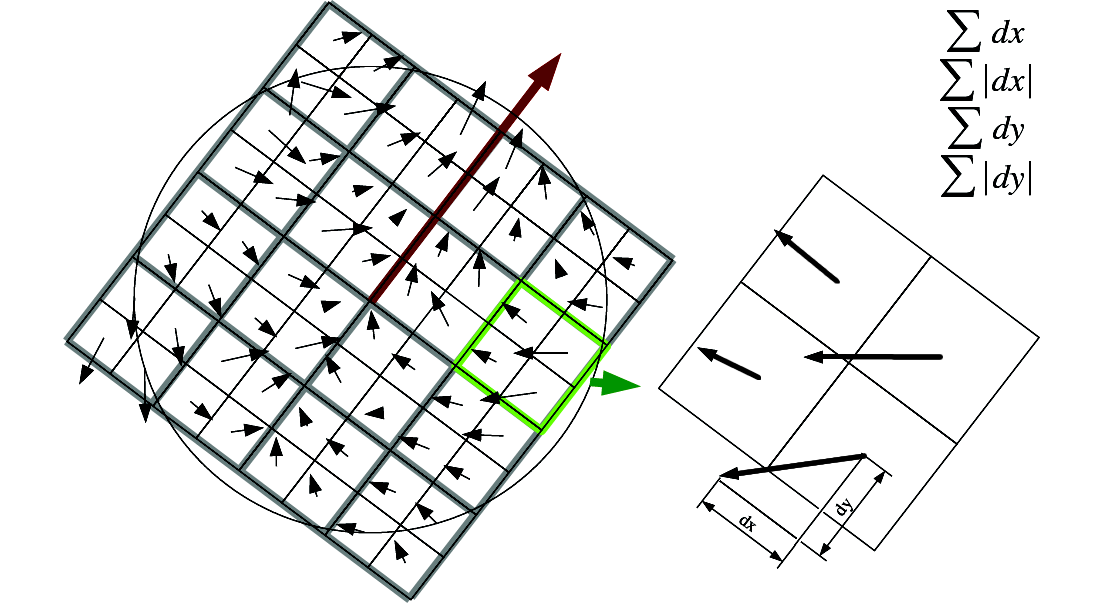
\includegraphics[width=0.5\textwidth]{SURF2.png}
  \caption{Respuestas de Haar en las sub-regiones alrededor del punto de interés. (Bay)}
  \label{fig:surf2}
\end{figure}

\paragraph{Matching entre puntos clave}

Esta sección, al igual que en el caso del descriptor SIFT, representa la correspondencia de los puntos clave identificados entre dos imágenes. La estrategia utilizada para establecer las correspondencias entre los puntos clave de ambas imágenes es la de ``el vecino más próximo'' descrita anteriormente. En el caso del descriptor SURF, el umbral relativo es fijado con un valor de 0,7.

\begin{figure}
  \centering        
  
\includegraphics[width=0.5\textwidth]{SURF1.png}
  \caption{Estimación de la orientación sobre puntos de interés. (Bay)}
  \label{fig:SURF1}
\end{figure}

\section{Tracking}
En contraste con la detección, que estima la pose de la cámara en una imagen, el tracking es el seguimiento del objeto (y la estimación de la pose de la cámara respecto a ese objeto) en una secuencia de fotogramas.

El procedimiento a seguir es la de identificar ``puntos clave'' visualmente significativos en un frame que podamos encontrar de forma fiable de nuevo en el siguiente. El procedimiento de tracking se basa en encontrar una cantidad suficiente de estas correspondencias de puntos entre los frames.

El tracking, es un problema complejo debido a la pérdida de información causada por la proyección del mundo 3D en una imagen 2D, la calidad de la imágenes obtenidas, fondos difíciles de segmentar, oclusiones totales o parciales, cambios en la iluminación y la exigencia de para trabajar en tiempo real. 

Para construir un buen sistema de tracking, es deseable que cumpla con los siguientes requisitos:

\begin{description}
\item [Robusto] Incluso en condiciones complicadas, como fondos difíciles de segmentar, cambios de iluminación, oclusiones o movimientos complejos, un algoritmo de tracking debe ser capaz de seguir al objeto de interés.

\item [Adaptable] Adicionalmente a los cambios de entornos que se puedan producir, el objeto en sí también puede sufrir cambios. Esto requiere que el algoritmo tenga algún mecanismo de adaptación para el seguimiento del objeto según la apariencia que tenga en cada momento.

\item [Cómputo en tiempo real] Para obtener una sensación fluida y que el ojo humano no perciba retrasos en la imagen, al menos debemos trabajar y procesar 15 imágenes por segundo. Por tanto, es necesario que el algoritmo sea rápido y esté optimizado.

\end{description}

Desde el punto de la información obtenida para el cálculo de la pose de la cámara, las técnicas de tracking se pueden se dividir en dos tipos:

\begin{description}
\item [Tracking por detección o búsqueda (by matching).] El cálculo de la posición y orientación de la cámara (camera pose) se realiza en cada frame por correspondencia entre la imagen de entrada y otra de referencia mediante una técnica de detección. La información de anteriores “poses” de la cámara no son tenidas en cuenta para la estimación de la nueva pose. El calculo de la pose mediante arboles aleatorios \cite{Lepetit} y estructuras no jerárquicas \cite{Ozuysal} son ejemplos de este tipo de enfoque.

\item [Tracking mediante tracking.] Para el calculo, la pose previa es utilizada como pose inicial para el cálculo de la posición y orientación actual. Una vez que se detectado un objeto, se hace un seguimiento de los puntos claves del objetos en el siguiente fotograma \cite{Wagner}, o minimizan la diferencia entre dos imágenes consecutivas \cite{Park} y analizan el cambio no lineal de iluminación producida \cite{Dame}. La mayoría de estos enfoques se basan en la minimización del desplazamiento de la cámara entre dos imágenes sucesivas.

\end{description}

Otra clasificación de los métodos de tracking disponibles puede dividirse en dos clases: basado en detección de características y basados en detección de modelos.

\subsection{Tracking por detección de características \emph{(feature-based)}}
En el mundo de la visión artificial una característica (feature) es una zona de la imagen que un algoritmo de tracking puede detectar y seguir a lo largo de múltiples frames. Normalmente las características suelen ser bordes, esquinas, zonas mas brillantes u oscuras en función del algoritmo de tracking en particular.

En lugar de utilizar marcadores de referencia, la estimación de la pose de la cámara se puede realizar mediante la extracción de características naturales, como puntos, líneas, bordes o texturas. Esta línea de investigación también ha sido ampliamente estudiado. Park \cite{Park3} presenta un método en el que utiliza las características naturales como una extensión en el tracking de características artificiales. Después de realizar el cálculo de la estimación de la pose de la cámara mediante características visuales conocidos, el sistema sistema adquiere dinámicamente características naturales adicionales y los utiliza para la actualización continua de la estimación de la nueva pose. De esta manera proporciona un seguimiento robusto, incluso cuando las marcas originales originales ya no están a la vista.

\subsubsection{Optical Flow}
El \emph{Optical Flow} o flujo óptico juega un papel importante en la estimación y descripción del movimiento, por lo cual es comúnmente utilizado en tareas de detección, segmentación y seguimiento de objetos móviles en una escena a partir de un conjunto de imágenes. 

El flujo óptico puede ser definido como el movimiento aparente de los patrones de intensidad en una imagen. La palabra aparente indica que el movimiento espacial de los objetos (campo de movimiento) puede coincidir o no con el flujo estimado. No obstante, en situaciones en las cuales el movimiento de los objetos implica un movimiento de sus patrones de intensidad en el plano imagen, el flujo óptico puede ser directamente relacionado con el movimiento de los objetos en la escena. La mayoría de las técnicas existentes para la estimación del flujo óptico se puede clasificar en 4 categorías: las basadas en gradientes espacio-temporales, las basadas en comparación de regiones, las basadas en fase y las basadas en energía.

En todas las estrategias de estimación de flujo óptico se parte de la hipótesis de que los niveles de gris permanecen constantes ante movimientos espaciales en un tiempo dado. Dicha hipótesis da lugar a la ecuación general de flujo óptico, donde $I(x, y, t)$ corresponde a la intensidad en niveles de gris del píxel $(x,y)$ de la imagen $I$ en el tiempo $t$. 
\begin{equation}
  I(x,y,t) = I(x+dx,y+dy,t+dt)
\end{equation}

Expandiendo la ecuación anterior en series de Taylor sobre el punto $(x,y,t)$
\begin{equation}
  I(x,y,t) = I(x,y,t) + dx \frac{\partial I}{\partial x}+dy\frac{\partial I}{\partial y} + dt \frac{\partial I}{\partial t} + \epsilon
\end{equation}

donde $\epsilon$ contiene la información de las derivadas de orden superior. Si se asume $\epsilon$ despreciable, la ecuación de flujo óptico puede reescribirse como
\begin{equation}
  I_xu +I_yv+I_t = 0
\end{equation}
donde $(u,v)$, con $u = dx/dt$ y $v = dy/dt$ , corresponde al vector de flujo óptico y, $I_x$ y $I_y$ son las derivadas parciales horizontal y vertical de la imagen, respectivamente. Para cada píxel $(x,y)$ de la imagen, en el tiempo $t$, puede plantearse la ecuación anterior, sin embargo no existe una única solución para esta ecuación. Diferentes restricciones pueden emplearse para estimar el flujo óptico en la imagen. Horn y Shunck en \cite{Horn} restringen el flujo óptico en la imagen a variar suavemente, por lo que la ecuación es minimizada junto a un término de regularización que penaliza los cambios abruptos del flujo. Lucas y Kanade (LK) \cite{LKanade} proponen un método alternativo que se describe a continuación el cual puede ser implementado de forma más eficiente que el propuesto en \cite{Horn}. Las técnicas propuestas en \cite{Horn} y \cite{LKanade} se basan en gradientes espacio-temporales pues minimizan la ecuación anterior. 
\begin{figure}
  \centering
  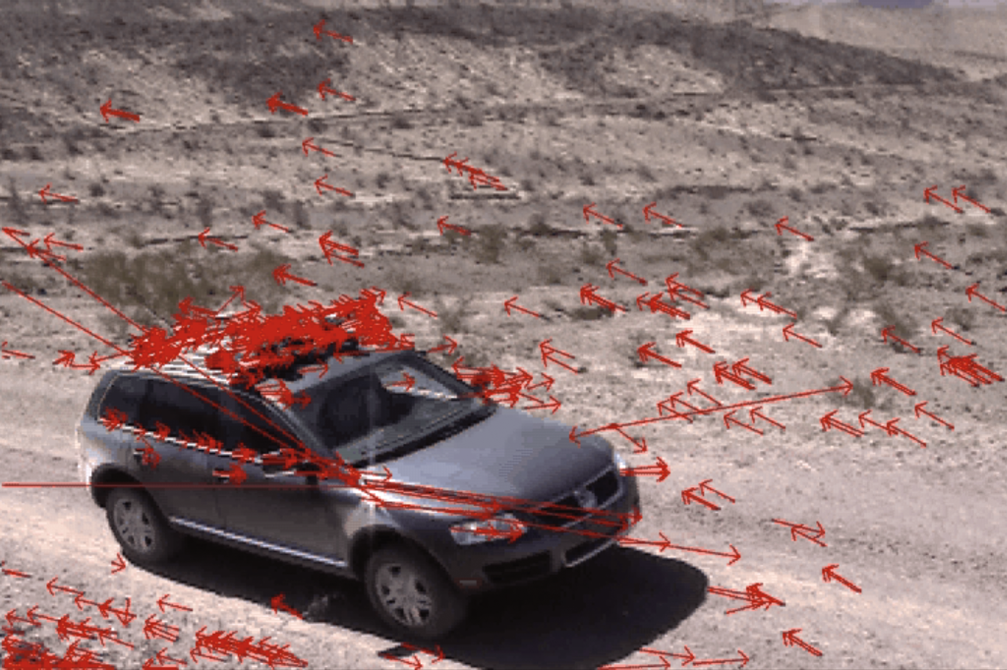
\includegraphics[width=0.8\textwidth]{LK.png}
  \caption{Lucas-Kanade: Seguimiento de puntos. (David Stavens)}
  \label{fig:overviewLK}
\end{figure}

\paragraph{Lucas-Kanade}
Este método asume que el flujo óptico es constante sobre una región. Sea $R$ una región de la imagen y $(u,v)$ su vector de flujo óptico asociado, entonces se cumple para cada píxel de la región, es decir
\begin{equation}
  I_x(p_i)u+I_y(p_i)v = -I_t(p_i) \quad  \forall p_i \in R
\end{equation}
Organizando el conjunto de ecuaciones en forma matricial
\begin{equation}
  A=
  \begin{bmatrix}
    I_x(p_1) & I_y(p_1) \\
    I_x(p_2) & I_y(p_2) \\
    \vdots  & \vdots  \\
    I_x(p_n) & I_y(p_n) 
  \end{bmatrix}
  \quad
  d=
  \begin{bmatrix}
    u\\
    v
  \end{bmatrix}
  \quad
  b = -
  \begin{bmatrix}
    I_t(p_i) \\
    I_t(p_2) \\
    \vdots  \\
    I_t(p_n)
  \end{bmatrix} 
\end{equation}

donde la matriz $A$ contiene las derivadas espaciales de la imagen, el vector $d$ corresponde al vector de flujo óptico $(u,v)$ y el vector $b$ contiene las derivadas temporales de la imagen.

Pre-multiplicando (3) por la transpuesta de $A$ se tiene
\begin{equation}
  A^T A d =A^T b
\end{equation}
donde el vector de flujo óptico es encontrado como 
\begin{equation}
  d= (A^T A)^{-1} A^T b
\end{equation}
El cálculo del flujo óptico implica la inversión de la matriz 
\begin{equation}
  A^TA=
  \begin{bmatrix}
    \sum I_x I_x  & \sum I_x I_y \\
    \sum I_y I_x  & \sum I_y I_y      
  \end{bmatrix}
\end{equation}

por la cual la solución existe si la matriz $A^TA$ es invertible y bien condicionada. Shi y Tomassi definen en [13] las propiedades que debe cumplir una región para que el flujo óptico se estimado apropiadamente utilizando la técnica de LK. Sean $\lambda_1$ y $\lambda_2$ los valores propios de la matriz  $A^TA$ para cierta región $R$ de la imagen, entonces se debe cumplir que:
\begin{itemize}
\item $min(\lambda_1 , \lambda_2) > \lambda_{min} \in R^+$ , lo cual garantiza que $A^TA$ es invertible y la región no es ruidosa.
\item $\lambda_1 /\lambda_2 < \tau$, lo que garantiza que $A^TA$ está bien condicionada y no se presenta bordes en una sola dirección
\end{itemize}

Bajo estas 2 condiciones el flujo óptico puede ser apropiadamente estimado. En la práctica existen ciertos factores que pueden inducir errores en la estimación. Entre ellos se encuentran la variación temporal de los niveles de gris sobre la región, desplazamientos grandes de la región entre las imágenes consecutivas e incoherencia de movimiento. El primero es independiente de la técnica de LK pero los otros 2 factores pueden ser controlados seleccionando un tamaño apropiado para la región R. Una región pequeña en comparación al tamaño del objeto garantiza una consistencia en el movimiento de las intensidades de gris, sin embargo si el objeto se desplaza rápidamente, éste puede salir de la región lo que produce un error en la estimación del flujo óptico. Por tal motivo existe un compromiso en el tamaño de la región R, el cual puede ser manejado con una implementación piramidal que estime  secuencialmente el flujo en diferentes escalas. En \cite{Bouguet} se presenta una implementación piramidal de la técnica de LK en la cual el flujo óptico es calculado recursivamente sobre versiones de diferentes escalas de las imágenes. En principio el flujo es estimado sobre imágenes en una escala baja para permitir grandes desplazamientos, posteriormente la escala se reduce para realizar una estimación más precisa  y evitar inconsistencias de movimiento. El tamaño de la región se mantiene fijo sobre todas las escalas.

\subsection{Tracking por detección modelos \emph{(model-based tracking)}}
La tendencia más reciente en las técnicas de tracking es el basados en modelos. Estas técnicas utilizan explícitamente un modelo de las características de los objetos rastreados, como por ejemplo, un modelo CAD 2D o un patrón del objeto basado en sus características distinguibles. El primer trabajo basado en modelos fue obra de Comport \cite{Comport} que en 2003 que utilizó una aproximación visual porción adaptada de la robótica para el cálculo de la cámara pose de una gama de características de modelo ( líneas, círculos , cilindros y esferas). 

\section{Reconocimiento y análisis de documentos}

\subsection{Texto y documentos}
En general, podemos considerar que cualquier escena o imagen que tenga un contenido textual como si fuera un documento. Esto incluiría tanto un libro, la matricula de un vehículo o un cartel en una pared. La mayoría de trabajos mediante cámaras están basados en la extracción de texto en imágenes fijas o secuencias de vídeo en las que los autores denominan imágenes naturales, en lugar de imágenes donde el texto está estructurado como los documentos. Ambos enfoques tienen sus desafíos y distintos modos de acometerlos, pero el objetivo final de todos es la de dotar a las cámaras la capacidad de lectura.

En el caso de documentos estructurados, que es el del dominio de este trabajo, las imágenes suelen ser documentos impresos como artículos, cartas, formularios o páginas de libros, donde gran parte de la imagen se asume que es texto, pero también puede contener figuras, diagramas e incluso algunos autores han tratado con anotaciones escritas a mano \cite{Chen}

\subsection{Identificación y recuperación de documentos}
Aunque hoy en día la mayor parte de la producción de información en forma de documentos se realiza por medio de herramientas informáticas (procesadores de texto, correo electrónico, etc.), puede ocurrir, y de hecho será un caso muy habitual, que la información no se restrinja a documentos actuales, ya automatizados, sino que se encuentre impresa. Incluso puede ocurrir que nos interese disponer sólo de la información antigua (archivos y manuscritos).

En estos casos para conseguir una gestión eficaz y ágil, es necesario digitalizar previamente estos documentos para incorporarlos al sistema que tenga implementado la organización.

Las primeras aplicaciones se basaban en el paradigma de reconocimiento de caracteres (OCR), donde se utilizaban estas técnicas para realizar un análisis del contenido informativo de los documentos y utilizarlo para su clasificación y almacenamiento. 

La recuperación de objetos (también nombrada por otros autores reconocimiento o identificación) se incorpora recientemente en la detección de tal manera que un objeto es capturado en una imagen, recuperado de una base de datos y su pose inicial se calcula simultáneamente \cite{Pilet}

El desarrollo de la investigación realizada en este ámbito se inició con los métodos que utilizaban marcas especiales en el documento, como códigos de barras \cite{Graham} o glifos para vincular contenido electrónico con las imágenes capturadas \cite{Hecht}. Los inconvenientes de estos enfoques es que es necesario modificar el formato y la apariencia del documento para introducir las marcas, que en algunos casos pueden distraer al usuario del contenido del documento. Por otro lado, un documento válido para el sistema al que no se le hayan incluido previamente estas marcas, no será detectado y vinculado con la información a recuperar.

La utilización del teléfono móvil y otros dispositivos portátiles para la identificación de documentos ha hecho que publiquen diversos artículos con algoritmos y métodos que parten de las propias limitaciones de estos dispositivos como es la baja capacidad de computo, la calidad de las imágenes capturadas, en muchos casos borrosas, y la captura parcial del documento.

Las técnicas de identificación y recuperación de documentos se pueden dividir en dos categorías \cite{Peng}: basados en la búsqueda de coincidencias de características locales y las que, además de lo anterior, utilizan la distribución del contenido dentro de la página.

\subsubsection{Basados en la búsqueda de coincidencias de características locales (feature matching)}
Algunos autores proponen técnicas de detección basados en la extracción de características invariante similares a SIFT \cite{Lowe} o SURF \cite{Bay} en trabajos como \cite{Yang} \cite{Psyllos} \cite{Brown} aplicadas a imágenes naturales y en alta resolución. Sin embargo, como indican Uchiyama y Saito \cite{Uchiyama}, estos métodos no funcionan correctamente para la identificación de documentos, ya que no presentan zonas de textura y se producen patrones binarios repetitivos (el texto de un documento cumple esta disposición). 

Mediante una variación del proceso inspirado en la metodología de Lowe \cite{Lowe} y Bay \cite{Bay}, Augereau \cite{Augereau} obtiene buenos resultados sobre documentos semi-estructurados (billetes de tren, tickets,...) realizando una selección de los puntos extraídos y una adaptación del algoritmo RANSAC para la validación de supuestos aciertos en la comparación.

\begin{figure}
  \centering
  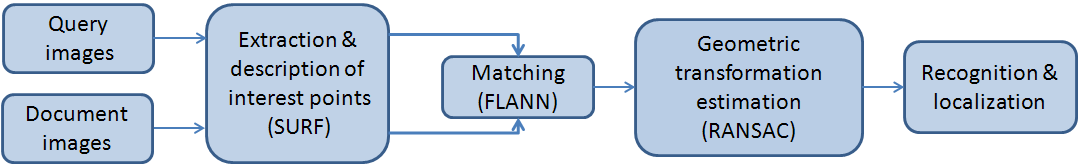
\includegraphics[width=0.9\textwidth]{standardObject.png}
  \caption{Proceso habitual para reconocimiento de imágenes mediante descriptores SURF (Augereau)}
  \label{fig:extraccionSt}
\end{figure}

\begin{figure}
  \centering
  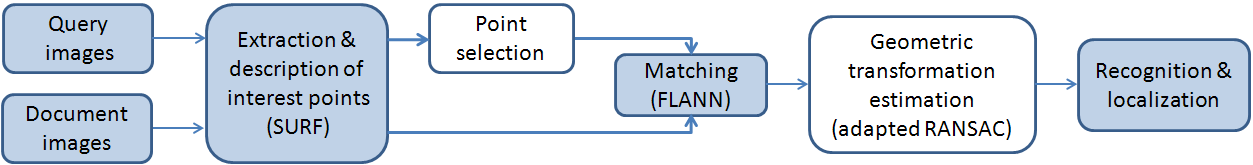
\includegraphics[width=0.9\textwidth]{adaptedObject.png}
  \caption{Proceso adaptado para reconocimiento de documentos mediante SURF (Augereau)}
  \label{fig:extraccionAd}
\end{figure}

El algoritmo tiene una alta tasa de recuperación y precisión, es robusto a las deformaciones que pueda tener la imagen (perspectiva) y no necesita ningún paso previo de segmentación, pero no funciona ante grandes secciones de texto y la identificación es para obtener documentos similares (no idénticos) a la imagen utilizada como consulta.

En PaperUI, Liu y Liao \cite{LiuLiao} implementan hasta siete enfoques distintos para identificar un documento: códigos de barras, micro-patrones ópticos, codificación oculta, huella digital, reconocimiento óptico de caracteres, detector de características locales como SIFT y FIT (una variación de SIFT), incluso tecnología RFID. Sin embargo PaperUI no es capaz de manejar bases de datos de gran tamaño porque el almacenaje de los vectores de características de SIFT requiere gran cantidad de memoria. 


\subsubsection{Basados en combinación coincidencias de características locales y la distribución del contenido dentro de la página}
Para superar las limitaciones, que tienen los enfoques anteriores en el uso específico de imágenes de documentos, otros autores proponen metodologías diseñadas para la recuperación de documentos, haciendo uso explícito de las características inherentes de la estructura del documento y el texto que contiene.

En su articulo, Liu y Doermann \cite{Liu}, presentan un método de recuperación basado en pares y tríos de tokens. En este método, se captura una página mediante un teléfono móvil y se envía a un servidor para recuperar el documento correspondiente. La aplicación ha sido desarrollada para trabajar con bases de datos de gran tamaño, sin embargo, se necesita mucho tiempo de procesamiento, alrededor de 4 segundos por consulta. Este tiempo de respuesta  supone un punto bastante negativo para considerarlo introducir en aplicaciones en tiempo real.

\emph{HotPaper} de Erol \cite{Erol}, es otro método que utiliza las características locales extraídas del texto del documento y su distribución denominado \emph{Brick Wall Coding Features (BWC)}. BWC define una característica local mediante la delimitación de palabras. Esta codificación es invariante a cambios de escala y robusta ante ligeras distorsiones de la perspectiva. El tiempo de procesamiento es rápido, alrededor de 300 ms por consulta y puede reconocer documentos a partir de imágenes con tan solo 4-5 líneas de texto y tamaños de imagen de 176 x 144. Como inconvenientes presenta problemas de escalabilidad, ya que el tamaño de la base de datos es muy pequeña, menos de 5000 páginas y la tasa de precisión es sólo alrededor del 60\%. 

Utilizando el mismo enfoque, pero utilizando otra codificación para generar los descriptores a partir de los \emph{bounding boxes}, Moraleda \cite{Moraleda} mejora la precisión hasta casi el 90\% y la escalabilidad para poder trabajar hasta con 500.000 documentos almacenados. 

\begin{figure}
  \centering
  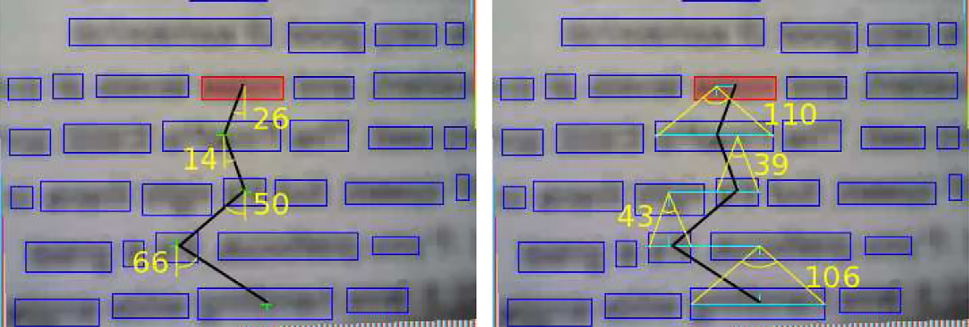
\includegraphics[width=0.9\textwidth]{bwcBounding.png}
  \caption{BWC: \emph{Bounding Boxes} en un fragmento de texto  (Moraleda)}
  \label{fig:extraccionAd2}
\end{figure}

Nakai y Kise proponen un método llamado \emph{Locally Likely Arrangement Hashing (LLAH)}, que utiliza el centro de una palabra como un punto característico y calcula descriptores locales basados en estos puntos\cite{Nakai}. LLAH tiene una alta escalabilidad y el esquema de indexación y recuperación empleado es extremadamente rápido. Los autores han confirmado que LLAH tiene una tasa de acierto del 99\% y con un tiempo de procesamiento de 50 ms en una base de datos de 20 millones de páginas.

En el algoritmo LLAH original, el movimiento de la cámara está restringido, ya que los cambios en el punto de vista causan variaciones en los descriptores locales. Uchiyama \cite{Uchiyama2} salva esta limitación estudiando el comportamiento de los descriptores al variar el punto de vista y actualizándolos continuamente. Como resultado, el método puede aplicarse a varias posiciones e inclinaciones de la cámara, permitiendo un movimiento de la cámara mucho más flexible. Iwata \cite{Iwata} extiende también el algoritmo LLAH para su utilización con imágenes parciales del documento en las que aparezcan tan sólo 4 o 5 líneas de texto. Por otra parte, a través del proceso de recuperación, LLAH puede estimar la \emph{pose} de la imagen de búsqueda en el documento electrónico, que es muy útil para mostrar información relevante sobre el documento.

Esta técnica también ha sido aplica para el desarrollo de marcadores de puntos aleatorios \cite{Saito}

\subsection{Locally Likely Arrangement Hashing (LLAH)}

LLAH es un método ampliamente utilizado para la recuperación de imágenes de documentos. El algoritmo se ha tomado como base para otras aproximaciones, revisado y mejorado, tanto por sus autores, como por otros investigadores. En este apartado estudiaremos el algoritmo original que presentaron los autores \cite{Nakai0}

\begin{figure}
  \centering
  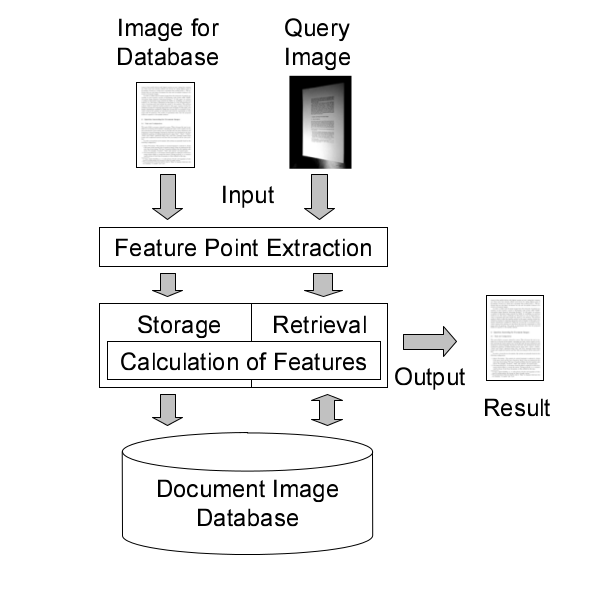
\includegraphics[width=0.6\textwidth]{LLAHesquema.png}
  \caption{LLAH: Visión General del proceso (Nakai y Kise)}
  \label{fig:overview}
\end{figure}

La Figura \ref{fig:overview} muestra un esquema general del proceso. En la etapa de extracción, la imagen se transforma en un conjunto de puntos de características. A continuación, los puntos se pasan a la etapa de almacenamiento o de recuperación (en función de la tarea  realizar). Estos pasos comparten la etapa de cálculo de características. En la etapa de almacenamiento, cada punto se almacena de forma independiente en la base de datos de imágenes de documentos usando su característica. La imagen es indexada utilizando cada uno de los puntos de características. En el paso de recuperación, se accede al  documento mediante las búsqueda de los puntos encontrados.

\subsubsection{Extracción de puntos característicos}
Un requisito importante en la extracción de características es que los puntos se deben obtener de forma idéntica, bajo la misma distorsión de perspectiva, ruido y resolución. Para satisfacer este requisito, emplean como puntos característicos los centroides de las regiones que ocupan las palabras del documento.

En primer lugar, se realiza una umbralización adaptativa a la imagen de entrada (Fig.\ref{fig:extraccion}(a)) y así obtener una imagen binaria (Fig.\ref{fig:extraccion}(b)). A continuación, se desenfoca usando un filtro gaussiano. Seguidamente, la imagen desenfocada es umbralizada de nuevo (Fig.\ref{fig:extraccion}(c)). Las regiones resultantes se supone que son espacios ocupados por palabras, y por último, (Fig.\ref{fig:extraccion}(d)) se extraen los centroides de las regiones para utilizarlos como puntos característicos.

\begin{figure}
  \centering
  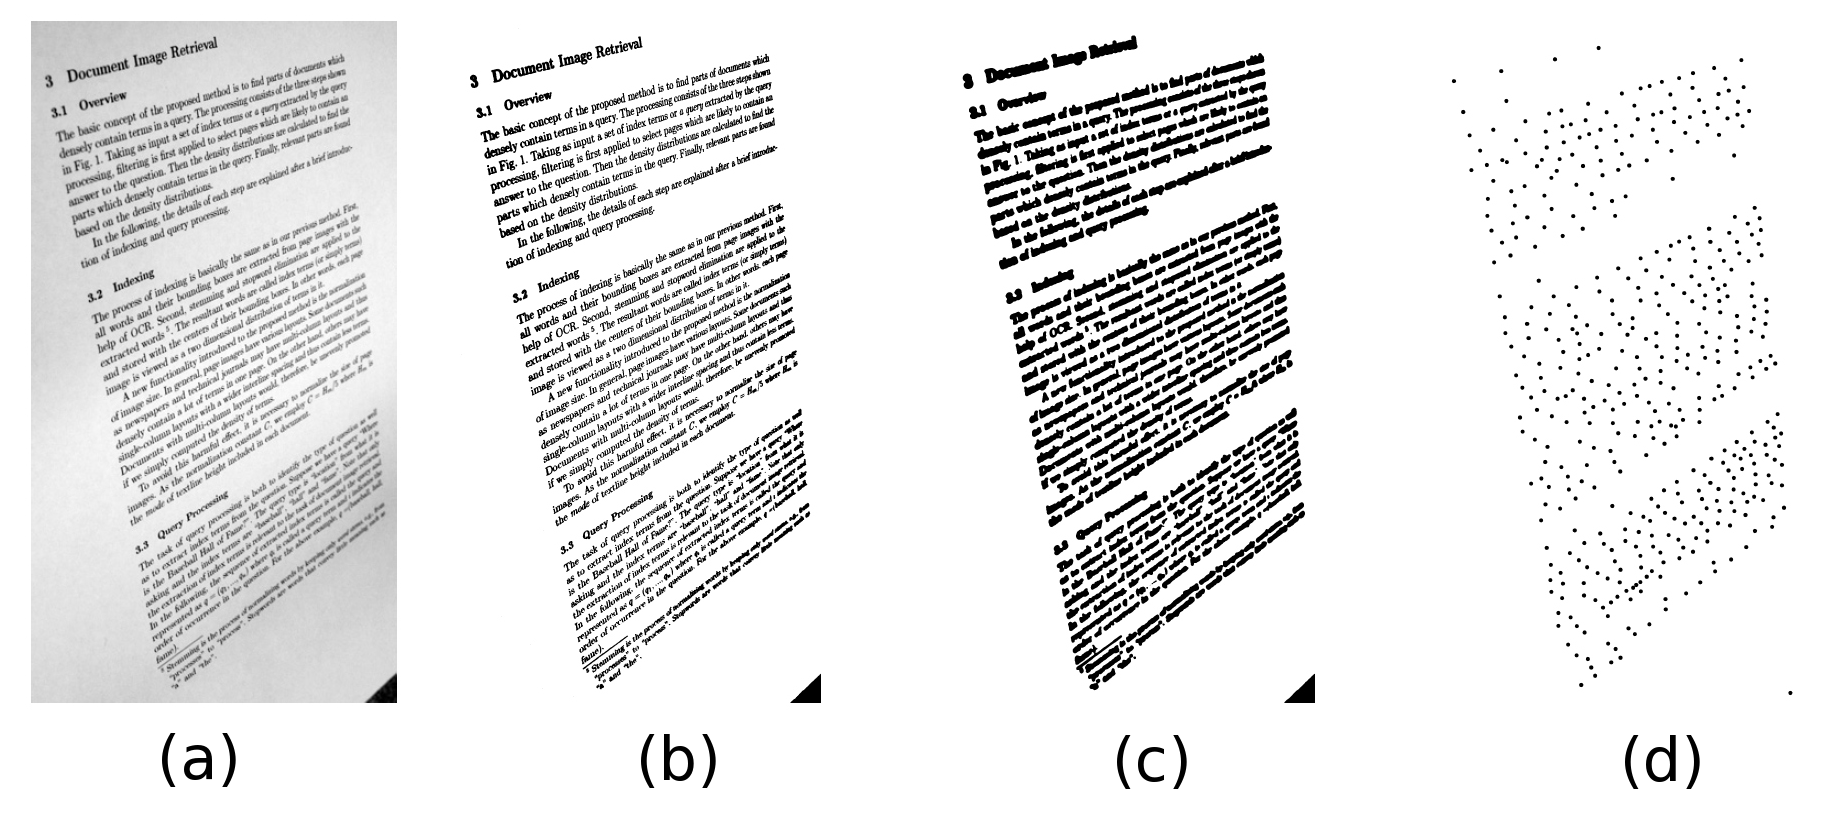
\includegraphics[width=0.9\textwidth]{LLAH.png}
  \caption{LLAH: Extracción de características (Nakai y Kise)}
  \label{fig:extraccion}
\end{figure}

\subsubsection{Cálculo de Descriptores locales}
Los descriptores de LLAH tiene las siguientes características:
\begin{itemize}
\item Se define un descriptor para cada punto característico. Con el fin de obtener robustez y disponibilidad en situaciones de oclusión, un descriptor tiene una localización.
\item Se calcula utilizando invariantes geométricos. Una invariante afín se define mediante cuatro puntos coplanares ABCD de la siguiente manera:
  \begin{center}
    $ \dfrac{P(A,C,D)}{P(A,B,C)} $
  \end{center}
  donde P(A,B,C) es el área de un triángulo con vértices A, B y C.
\item Un descriptor consta de más de una invariante geométrico. Para aumentar el poder de discriminación de un descriptor, se utilizan múltiples invariantes afines calculados a partir de varios puntos característicos. Cómo un invariante afín se calcula a partir de cuatro puntos, podemos calcular más de una invariante partir de más de cuatro puntos característicos. En concreto, un descriptor es $(r_{(0)},...,r_{_{m}C_{4}-1})$ calculado a partir de los $m$ puntos contiguos donde $r_{(i)}$ es una invariante afín. Se utilizan todas las posibles combinaciones de cuatro puntos $m$.
\item Se calculan más de un descriptor para cada punto característico. Con el fin de hacer frente a los errores de la extracción de puntos característicos,se calculan múltiples descriptores a partir $n (>m)$ puntos mas cercanos. En concreto, se calculan $_{n}C_{m}$ descriptores, todas las combinaciones posibles de $m$ puntos contiguos sobre $n$ puntos totales.
\end{itemize} 

\begin{figure}
  \centering
  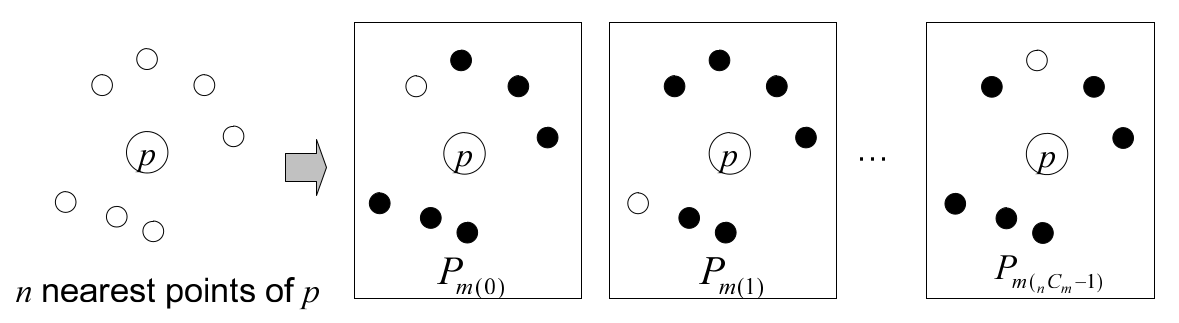
\includegraphics[width=0.9\textwidth]{nearestLLAH.png}
  \caption{LLAH: Todas la posibles combinaciones de \textit{m}(=6) puntos de los \textit{n}(=7) puntos contiguos a \textit{p} (Nakai y Kise)}
  \label{fig:nearest}
\end{figure}

\subsubsection{Almacenamiento y Recuperación}
En LLAH las imágenes se almacenan y recuperan mediante una tabla hash. En primer lugar se calculan y almacenan los descriptores de la imagen de forma preliminar. Cuando se da una imagen para recuperar, se calculan los descriptores de la consulta y se buscan y contabilizan los documentos posibles en los que coincidan el mismo descriptor. Finalmente, el documento que obtiene el mayor número de votos (descriptores encontrados)  es devuelto como resultado del proceso de recuperación


\subsection{Limitaciones en la identificación de documentos}
El análisis de documentos mediante cámaras tiene una serie de ventajas sobre aquellos que están basados en la adquisición mediante escáner. Las cámaras son pequeñas y fáciles de transportar. También se pueden utilizar en cualquier entorno y sobre documentos que por su formato sean difíciles de manipular en un escáner como periódicos, libros, o manuscritos antiguos. Incluso para capturar texto que no se encuentra en papel, como carteles en fachadas, o texto que se encuentre el objetos que se muevan por la escena.

En la mayoría de casos, los escáneres obtienen mejor calidad en la captura de calidad que las realizadas mediante cámaras, pero los sistemas basados en cámaras son mucho más flexibles y portables. 

\subsubsection{Problemática asociada}
Casi todos los algoritmos de reconocimiento de documentos obtienen grandes resultados partiendo de imágenes limpias, en alta resolución y con contrastes claramente definidos entre el texto y el fondo. Sin embargo, mediante la captura con cámaras debido a su naturaleza, a la forma en que se realiza la captura y el entorno en que nos encontremos se presentan una serie de dificultades que deben ser tenidas en cuenta.  
\begin{description}
\item[Baja resolución] Las imágenes obtenidas con las cámaras suelen estar en baja resolución, bien por las limitaciones del sensor, o por que la capacidad de computo del dispositivo que la contiene es limitada. Mientras que con un escáner es normal trabajas con una resolución de entre 150 a 600 dpi, el mismo texto en una captura con una cámara rodaría los 50 dpi.
\item[Iluminación no uniforme] La cámara, al contrario que el escáner no tiene control de la iluminación de la escena. En la captura mediante cámaras es normal encontrarse con iluminación no uniforme, varias fuentes de luz con temperaturas de color diferentes, sombras o reflejos que degradan la calidad de la imagen.
\item[Distorsión por perspectiva] Al capturar el texto sin estar la cámara paralela al plano en el que se encuentra el documento, se está produciendo una distorsión por perspectiva. Esto provoca que el texto presente distintos tamaños a lo largo de la imagen o que se produzca una deformación que impida el correcto reconocimiento de los caracteres. 
\item[Distorsión de la lente] Las cámara incorporadas a los teléfonos móviles suelen tener una distancia focal menor para obtener un mayor ángulo de visión. La consecuencia de esto es que la lente exagera la perspectiva de los objetos, provocando mayor distorsión en las líneas cuanto más cerca se encuentre la lente del objeto.
\item[Fondos complejos] El caso ideal para la extracción de texto es que el fondo sea totalmente uniforme y con contraste diferenciado. Una mala iluminación provocará alteraciones de tono y contraste entre texto y fondo, que dificultará la segmentación el texto. 
\item[Zoom y autoenfoque] Las cámaras actuales están equipadas con sistemas de zoom y autoenfoque. Una captura en la que existan distintos planos de profundidad o una mala iluminación provocará que el sistema de autoenfoque tenga dificultades para estabilizarse y durante ese tiempo las imágenes sean borrosas o fuera de foco.
\item[Objetos móviles] Por la propia naturaleza de los dispositivos móviles se entiende que o bien el dispositivo o el objeto a fotografiar está en movimiento (o incluso ambos). Si la velocidad de obturación de la cámara no es lo suficientemente rápida, la imagen obtenida estará movida.
\item[Ruido del sensor] Para compensar entornos con poca luz, las cámaras aumentan la sensibilidad amplificando la señal generada por las celdas del sensor. Como estos elementos tienen una emisión de señal de base mas o menos fija, al capturar una señal lumínica débil y amplificarla, estamos amplificando también una buena porción de la emisión de datos aleatoria, con lo que se mezclará una cantidad de señal aleatoria sin contenido a la señal correspondiente a la imagen. Cuanto mayor sea la amplificación, más ruido se va a generar y peor calidad de imagen vamos a obtener. 
\item[Compresión de imagen] Normalmente la imagen obtenida por el sensor se almacena comprimida mediante algoritmos con perdida de información como JPEG. La utilización de ratios altos de compresión provoca que se generen artefactos y distorsiones apreciables que restan nitidez a la imagen.
\item[Algoritmos ligeros] El objetivo final es integrar los algoritmos de análisis en los dispositivos móviles. Se deben implementar algoritmos computacionalmente eficientes ya que en la mayoría de los casos los recursos disponibles como memoria  y la capacidad de computo son limitadas.
\end{description}



% Local Variables:
%  coding: utf-8
%  mode: latex
%  mode: flyspell
%  ispell-local-dictionary: "castellano8"
% End:

\chapter{Método de trabajo}
\label{chap:metodo}

\drop{E}{n} este capítulo se describe la metodología de desarrollo aplicada, sus ventajas y motivo de elección. También se listan y describen todas las herramientas utilizadas en el desarrollo, ya sean hardware o software.

Al final del capitulo se presenta la evolución del proyecto en base a la metodología empleada, los hitos conseguidos en cada fase, su complejidad y el tiempo empleado en cada una de ellas, detallando las iteraciones realizadas hasta conseguir la versión final del sistema. Igualmente se aportará información del rendimiento (profiling) del sistema en diferentes situaciones.

\section{Metodologia del desarrollo}
Para la construcción de un proyecto de cierta envergadura, como es el caso de un Trabajo Fin de Grado, la aplicación de un marco de trabajo para estructurar, planificar y controlar el proceso, es esencial para desarrollar software de calidad.

Las caŕacteristicas del proyecto, con requisitos con posibilidad de cambios y adaptaciones a lo largo de todo el proceso, el reducido ``equipo de desarrollo'' o la necesidad de obtener versiones incrementales que son testeadas y validas por el director de proyecto, hacen que la elección se decante hacia metodologias ágiles de desarrollo de software.

Los métodos ágiles, utilizan prácticas adaptativas (no basadas en predicciones), iterativas, centradas en la gente (clientes y programadores), orientadas a entregas incrementales, con mucha comunicación y necesitan que el cliente esté muy involucrado en el proyecto para recibir su feedback. El feedback continuo es indispensable para evitar que el cliente, con el software acabado, diga “es lo que pedí, pero no es lo que necesitaba”, algo habitual cuando se utiliza métodos clásicos.

En resumen, las principales características a las que deben dar forma los métodos ágiles son:
\begin{itemize}
\item \textbf{Incremental:} versiones pequeñas de software, con ciclos rápidos. 
\item \textbf{Cooperativo:} desarrolladores y cliente siempre en contacto constante.
\item \textbf{Directo:} el método en si es fácil de aprender y modificar, bien documentado.
\item \textbf{Adaptativo:} capaz de tolerar los cambios propuestos por el cliente.
\end{itemize}

Hay que tener en consideración la muy diferente naturaleza de los métodos ágiles. Mientras que Scrum se decanta por la gestión, otros como XP especifican las prácticas a seguir en el equipo, Pragmatic Programming da pautas para desarrollar un buen código, algunos como FDD no abarcan la totalidad del proceso de desarrollo, AgileUP surge como una versión ágil de RUP y propone EUP que es una ampliación para abarcar todo el ciclo de vida del software, etc.

Scrum se ha desarrollado para gestionar el proceso de desarrollo de sistemas. Aplica ideas de proceso industrial para controlar el desarrollo de los sistemas. Su enfoque reintroduce las ideas de flexibilidad, adaptabilidad y productividad. No define ninguna técnica de desarrollo de software específica para la fase de aplicación. Scrum se centra en cómo deben funcionar los miembros del equipo para que el sistema sea flexible y se adapte a unas condiciones
constantemente cambiantes.

\subsection{Fases de Scrum}
El proceso de Scrum consta de tres fases: pre-game, desarrollo o game y post-game.

A continuación se detallan las fases de Scrum según Schwaber y Beedle. La fase pre-game incluye dos subfases:
\begin{itemize}

\item \textbf{Pre-game}
El planteamiento incluye la definición del sistema a desarrollar y asegurar la financiación. Se crea una lista de acumulación o pila de producto, Product Backlog list conteniendo todos los requisitos conocidos hasta el momento. Los requisitos los puede originar el cliente, los programadores o los departamentos de ventas, marketing o atención al cliente. Se priorizan los requisitos y se estima el esfuerzo necesario para su desarrollo. La Product Backlog list se actualiza constantemente con puntos nuevos y más detalles, así como con estimaciones más exactas y el nuevo orden de prioridades. El planning también incluye la definición del equipo del proyecto, herramientas y otros recursos, la valoración de riesgos, necesidades de formación y la aprobación de la gestión de comprobaciones. En cada iteración, el equipo(s) de Scrum revisa la Product Backlog list actualizada. En la jerga de Scrum, se llaman paquetes a los objetos o componentes que necesitan cambiarse en la siguiente iteración.

En la fase de la arquitectura, se crea el diseño del sistema a alto nivel basándose en los requisitos actuales del Backlog. En el caso de una mejora a un sistema ya existente, se identifican los cambios necesarios en el backlog así como los problemas que puedan causar. En una reunión se revisa el diseño del plan para cumplir las propuestas. Además, se preparan los contenidos de las versiones que serán lanzadas. 

\item \textbf{Game}
Esta fase, la parte ágil de Scrum, se trata como una caja negra donde se espera lo imprevisible. Las diferentes variables técnicas y de entorno que pueden cambiar (calendario, calidad, requisitos, recursos, tecnologías, herramientas, e incluso métodos de desarrollo) se observan y controlan durante los sprints. En lugar de considerar estos puntos sólo al principio del proyecto, Scrum los controla constantemente para adaptarse a los cambios. En la fase de desarrollo, el sistema funciona en sprints o carreras cortas. Los sprints son ciclos iterativos donde se desarrollan o mejoran las funcionalidades para producir los nuevos incrementos. Cada sprint incluye las fases habituales de desarrollo del software: requisitos, análisis, diseño, desarrollo y entrega. La arquitectura y el diseño del sistema evolucionan durante el desarrollo del sprint. Un sprint dura de una semana a un mes. Puede haber de tres a ocho sprints, por ejemplo, antes de que el sistema esté listo para lanzarse. También puede haber más de un equipo que construya cada incremento.

\item \textbf{Post-game}
Contiene el cierre de la versión. Se entra en esta fase cuando se completan todos los requisitos. En este caso, no se incorpora ni mejora ninguna función. El sistema ya está listo para lanzarse (release) y ahora se integra, se pone a prueba y se documenta.
\end{itemize}

\subsection{Papeles y responsabilidades}
Los papeles en Scrum tienen tareas y propósitos diferentes durante el proceso y sus prácticas.

\begin{itemize}
\item \textbf{Scrum Master} Es responsable de asegurar que el proyecto se realiza según las prácticas, valores y reglas de Scrum y que progresa como estaba previsto. Actúa recíprocamente tanto con el equipo del proyecto como con el cliente. También es responsable de resolver cualquier impedimento para seguir trabajando tan productivamente como sea posible. 

\item \textbf{Propietario del producto} El propietario del producto es oficialmente responsable del proyecto, gestionando, controlando, y haciendo visible la Product backlog list. Es elegido por el Scrum Master, el cliente y la dirección. Toma las últimas decisiones de las tareas relacionadas con la Product backlog list, participa estimando el esfuerzo de desarrollo para los puntos del Backlog y los concreta en funcionalidades a desarrollar.

\item \textbf{Equipo de Scrum} El equipo de Scrum tiene autoridad para decidir las acciones pertinentes para organizarse y lograr lo propuesto en cada sprint. El equipo de Scrum está involucrado, por ejemplo, en estimar el esfuerzo requerido para cada parte, crear y revisar la Product Backlog list e identificar problemas a tratar.

\item \textbf{Cliente} El cliente participa en las tareas relacionadas con los puntos del Backlog para diseñar o mejorar el sistema.

\item \textbf{Director} La gestión o dirección toma la última decisión y se encarga de los documentos, normas y convenciones seguidas en el proyecto. La dirección también participa en identificar objetivos y requisitos. Por ejemplo, ayuda a seleccionar el product owner, valorar los progresos y reducir el Backlog con el Scrum Master.
\end{itemize}

\subsection{Elementos}
\subsubsection{Documentos}
\begin{itemize}
\item \textbf{Product Backlog} El Product Backlog define todo lo necesario en el producto final, basándose en los conocimientos de ese momento. Por tanto, define el trabajo a hacer en el proyecto. Incluye una lista ordenada por prioridades y actualizada de requisitos técnicos para que el sistema se haga o mejore. Los puntos del Product Backlog, por ejemplo, pueden incluir características, funciones, parches para bugs, defectos, peticiones de mejoras o actualizaciones de tecnología.
 
También se incluyen temas que requieren solución para poder hacer otros puntos de la lista. A la lista de backlog puede contribuir el cliente, el equipo del proyecto y los departamentos de ventas, marketing y atención al cliente.
Esta práctica incluye las tareas para crear la lista de backlog, actualizarla agregando, quitando o especificando puntos con sus respectivas prioridades. El Product Owner es responsable de mantener el Product Backlog.

\item \textbf{Sprint Backlog} Es el punto de partida para cada sprint, una lista de puntos de la lista del Product Backlog seleccionados para llevarse a cabo en el próximo sprint. El equipo de Scrum junto con el Scrum Master y el Product Owner seleccionan los puntos en la reunión para planear el Sprint, basándose en los puntos con prioridad y los objetivos de ese sprint. A diferencia del Product Backlog, el Sprint Backlog no se modifica hasta que el sprint (es decir, 30 días) termina.
 
Cuando todos los puntos del Sprint Backlog están completos, se prepara una nueva iteración del sistema. El registro incluye los valores que representan las horas de trabajo pendiente; en función de esos valores se acostumbra a elaborar un gráfico de quemado (se pueden ver ejemplos en el apartado de Crystal, 2.3), usados también en muchos otros métodos.
\end{itemize}
\subsubsection{Reuniones}
\begin{itemize}
\item \textbf{Reunión diaria de Scrum} Se organizan reuniones de Scrum diarias para seguir el progreso del equipo y planear las reuniones: qué se ha hecho desde la última reunión y qué se hará para la siguiente. También se ponen sobre la mesa problemas y otros asuntos que puedan aparecer en esta reunión diaria de unos 15 minutos. Se busca y soluciona cualquier deficiencia o imprevisto del proceso. El Scrum Master dirige las reuniones. La dirección (Management), también puede colaborar en la reunión.

\item \textbf{Reunión para plantear el Sprint} El Sprint Planning meeting consta de dos fases y la organiza el Scrum Master. En la primera fase, los clientes, usuarios, la dirección, el Product Owner y el equipo, eligen los objetivos y las funcionalidades del próximo sprint. En la segunda fase, el Scrum Master y el equipo concretan la manera de conseguir esos objetivos (product increment) en el siguiente sprint.

\item \textbf{Sprint review meeting} En el último día del sprint, el equipo y el Scrum Master presentan los resultados del sprint, (el incremento producido) a la dirección, clientes, usuarios y Product Owner en una reunión informal. Los participantes evalúan la evolución y deciden sobre las siguientes actividades. La reunión de la revisión puede revelar nuevos puntos e incluso cambiar la dirección tomada del sistema que se está construyendo.

Al final de cada iteración de treinta días hay una demostración a cargo del Scrum Master. Las presentaciones en PowerPoint están prohibidas. En los encuentros diarios, las gallinas deben estar fuera del círculo. Todos tienen que ser puntuales; si alguien llega tarde, se le cobra una multa que se destinará a obras de caridad. Se permite usar artefactos de los métodos a los que Scrum acompañe, por ejemplo Listas de Riesgos si se utiliza UP, Planguage si el método es
Evo, o los Planes de Proyecto sugeridos en la disciplina de Gestión de Proyectos de Microsoft Solutions Framework. No se permiten, en cambio, instrumentos como diagramas PERT, porque parten del supuesto de que las tareas de un proyecto se pueden identificar y ordenar.
\end{itemize}
\subsubsection{Sprint}
 El sprint consiste en adaptarse a las condiciones cambiantes del proyecto como requisitos, tiempo, recursos, conocimiento, tecnología, etc. El Equipo de Scrum se organiza para producir un nuevo incremento ejecutable en un sprint que dura aproximadamente un mes natural. Las herramientas activas del equipo son las reuniones para planear el sprint, el Sprint Backlog y las reuniones diarias de Scrum.



\section{Evolución del proyecto}

Para la resolución de este proyecto se ha optado por una aproximación en la que se complementan las mejores prácticas y técnicas recomendadas en Scrum, con sus patrones organizacionales como método de gestión y XP, con patrones de diseño, programación guiada por pruebas y refactorización, como metodología de desarrollo

2.2.3. La práctica
Scrum no requiere o proporciona ninguna práctica específica para el desarrollo del software. Sin embargo, requiere adoptar ciertas pautas y prácticas para evitar el caos causado por imprevistos y complejidades.
Las pautas de Scrum son:
• Equipos auto-dirigidos y auto-organizados. No hay manager que decida, sino “miembros del equipo”; la excepción es el Scrum Master que debe ser 50\% programador y que resuelve problemas, pero no manda. Los observadores externos pueden observar, pero no interferir ni opinar.
• Una vez elegida una tarea, no se agrega trabajo extra. En caso que se agregue algo, se recomienda quitar alguna otra cosa.
• Encuentros diarios con esta tres preguntas indicadas:
- ¿Qué has hecho desde la última reunión (día anterior)?
- ¿Has encontrado algún obstáculo?
- ¿Qué harás para la siguiente reunión (mañana)?
Se realizan siempre en el mismo lugar, en círculo. La reunión diaria impide caer en el problema señalado por Fred Brooks: “¿Cómo es que un proyecto puede retrasarse un año? Un día cada vez”.
• Iteraciones de 30 días; se admite que sean más frecuentes.
• Demostración a participantes externos al final de cada iteración.
• Al principio de cada iteración, planeamiento adaptativo guiado por el cliente.


2.9.1 Descripción del contexto 
El  equipo  de  desarrollo  lo  constituyen  los  autores  de  este  PFC,  estando  muy  habituados  a  trabajar  juntos,  con  experiencia  práctica  y  conocimientos  teóricos  en metodologías  ágiles.    Debido  al  tamaño  del  equipo  y  condiciones  del  mismo,  las  reuniones  diarias pierden su utilidad.  Como ya se ha mencionado, la figura del cliente esta desvirtuada y su función es desempeñada por el equipo de desarrollo. 
 Al comienzo de cada iteración el equipo se reunirá y creará el Iteration Backlog que consta de  un subconjunto de las User Stories del Product Backlog. Estas User Stories son seleccionadas  atendiendo a las prioridades del cliente. En esta reunión se descompondrá cada User Story del Iteration Backlog en tareas, estimando el tiempo necesario para llevarlas acabo. 


2.9.2 Descripción de las prácticas a utilizar 
Las prácticas XP que se van a utilizar son: 
Sentarse juntos 
Todo el desarrollo se llevará a cabo en un espacio que permita un trabajo cercano, cooperativo y  que  facilite  la  comunicación  directa.  En  las  ocasiones  en  las  que  ésto  no  sea  posible,  se utilizarán medios de videoconferencia como Skype o NetMeeting. 

Iteraciones cortas 
La  primera  iteración  será  de  15  días  de  duración,  y    en  ella  el  equipo  se  familiarizará  con  el  dominio  de  aplicación  y  las  tecnologías  a  utilizar.  También  se  definirá  en  buena  medida  la arquitectura del sistema.  
Las siguientes iteraciones serán de una semana. 
 
Integración continua. 
No se utilizarán herramientas que automaticen este proceso, no obstante, debido al tamaño  reducido del equipo y a la frecuencia de las integraciones (al menos una al día), esta tarea no resultará demasiado compleja. 

 Diseño incremental 
A  pesar  de  definir  buena  parte  de  la  arquitectura  en  las  primeras  iteraciones,  el  diseño  del  sistema evolucionará iteración tras iteración, sometiéndose a sucesivas refactorizaciones para mejorar su calidad.  

 Código compartido 
Esta práctica ha sido utilizada con anterioridad en el equipo de desarrollo. Cualquier miembro del mismo podrá introducir cambios en cualquier parte del código para mejorar su calidad. Sin olvidar que el presente desarrollo ágil se encuentra en el contexto de la elaboración de un PFC,  al  finalizar  cada  iteración  se  destinará  tiempo  a  completar  y  refinar  la  documentación obtenida del proceso

2.10.1 Product Backlog de la herramienta 
En  la  tabla  2.1  se  muestra  el  Product  Backlog  de  la  herramienta  que  constituye  la especificación completa de la funcionalidad de la misma. Recordemos que esta especificación viene determinada por las Historias de Usuario. 
Contiene el nombre de las Historias de Usuario y su identificador, así como la página de este PFC en la que se puede encontrar la información detallada de cada una.  

El Product Backlog define todo lo necesario en el producto final, basándose en los conocimientos de ese momento. Por tanto, define el trabajo a hacer en el proyecto. Incluye una lista ordenada por prioridades y actualizada de requisitos técnicos para que el sistema se haga o mejore. Los puntos del Product Backlog, por ejemplo, pueden incluir características, funciones, parches para bugs, defectos, peticiones de mejoras o actualizaciones de tecnología.
También se incluyen temas que requieren solución para poder hacer otros puntos de la lista. A la lista de backlog puede contribuir el cliente, el equipo del proyecto y los departamentos de ventas, marketing y atención al cliente.


2.10.2 Iteraciones 


2.10.2.1 Iteración 1 
La  iteración  1  está  comprendida  entre  el  1  de  julio  y  el  15  de  julio  del  2008.  Es  la iteración más larga debido a que en ella se llevan a cabo actividades que no se repetirán en el resto  de  iteraciones,  tales  como  familiarización  con  el  dominio  de  aplicación,  especificación inicial de la funcionalidad del sistema y esbozo de la arquitectura general del sistema. A continuación se mostrará el Backlog de la Iteración, las pruebas y el diseño generado en esta iteración. 




3.11.3 Reutilización del código 
Uno  de  los  principales  objetivos  que  se  persiguen  con  las  metodologías  ágiles  es  entregar  proyectos  en  tiempo  y  bajo  presupuesto.  En  otras  palabras,  se  pretende  minimizar  el  TTM (Time To Market) para lo que la reutilización del código constituye un aspecto muy importante, no  se  ha  de  perder  tiempo  reinventando  la  rueda  en  cada  proyecto.    Se  ha  de  tratar  de obtener  diseños  con  una  alta  modularidad,  reutilizando,  como  cajas  negras,  todos  los elementos  software  que  tengamos  y  necesitemos.  De  esta  forma  se  consiguen  sistemas  modulares en los que se reduce el coste de introducir modificaciones, reduciendo el coste de su mantenimiento;  Por  otro  lado  se  consigue  aumentar  el  repositorio  de  componentes  para futuros  proyectos,  con  todas  las  ventajas  que  ello  conlleva  (ver  Desarrollo  Basado  en Componentes). 

Se ha de tener en cuenta que no todos los elementos en un proyecto son reutilizables, puesto que es inevitable que algunos estén estrechamente ligados a condiciones particulares propias de cada dominio de aplicación, la modularidad tampoco ha de convertirse en una obsesión que nos obstaculice el avance del proyecto. Recordemos que si se conoce la mejor forma de hacer algo,  que  así  se  haga,  sino  que  se  haga  de  la  mejor  forma  conocida  para  la  que  se  tenga tiempo. 
  
\subsection{Concepto del software}
\subsection{Análisis preliminar de requisitos}
\subsection{Diseño general}
\subsection{Iteraciones}
En este capítulo se presenta toda la documentación generada para gestionar este proyecto de desarrollo. Esta documentación está estructurada en ocho iteraciones, tal y como se describió en el estudio teórico de las metodologías ágiles. 

\subsubsection{Iteracion 0}
Como punto de partida para la elaboración del estado del arte se realizo una revisión sistemática de las diferentes técnicas para la identificación de documentos y su recuperación de una base de datos. Como resultado de esta revisión se ha podido conocer las técnicas más empleadas, así como sus ventajas e inconvenientes. 

El claro ganador es LLAH (Locally Likely Arrangement Hashing) con casi un 40\% de utilización ya sea con su implementación inicial o implementaciones optimizadas creadas para salvar las limitaciones del algoritmo original, lo que lo hace aún mas potente y versatil.

Aunque los metodos basados en detección de descriptores de caracteristicas invariantes como SIFT, SURF, aparecen como muy utilizados, realmente no funcionan correctamente en identificación de documentos ya que no presentan zonas de textura y se producen repeticiones de patrones binarios (el propio texto cumple este patron). La mayoria son una variación del proceso inspirado en la metodologia de Lowe [SIFT], y en la que se obtienen buenos resultados sobre documentos semiestructurados realizando una selección de puntos extraidos y una adaptación del algoritmo RANSAC para la validación de supuestos aciertos en la comparación. El algoritmo tiene una tasa elevada de recuperación y precisión, es robusto a las deformaciones que pueda tener la imagen (perspectiva) y no necesita ningun paso previo de segmentación pero, como inconvenientes, no funciona ante grandes secciones de texto y la identificación que realiza es para obtener documentos similares (un ticket, un billete de tren,....) a la imagen utilizada como consulta.

Uno de los puntos del analisis de resultados, indica que al utilizar hardware con distinto rendimiento, es dificil tener mediciones normalizadas para todos los métodos. Como trabajo futuro se puede realizar para el gestor documental, la implementación de varios de los metodos mas utilizados y ofrecer un estudio comparativo completo al ejecutarse en la misma plataforma.

Existen varias implementaciones optimizadas sobre LLAH para salvar las limitaciones iniciales del algoritmo. Sería un trabajo futuro la tarea de buscar sólo las publicaciones que se hayan hecho sobre LLAH e intentar crear una implementación conjunta  con todas las optimizaciones. 

Elección del Proyector

Una vez recibida la raspberry se procede a la configuración del entorno de trabajo. Instalación de Raspbian, OpenCV, compiladores, editores y configuración del servicio de SSH para controlarla desde el puesto de trabajo.

\subsubsection{Iteración 1}
El objetivo de esta primera iteración es obtener una arquitectura básica que iremos completando y refinando en cada una de las sucesivas iteraciones.

Analisis
Partiendo de las premisas que tiene el proyecto ARgos de ser un sistema autonomo, de inicio automático, sin dispositivos como ratones y teclados, en el que la experiencia de usuario vendra en función de lo que se vaya detectando en cada fotograma. 
Las limitadas capacidades de la raspberry pi y la experiencia que otros programadores han tenido a la hora de trabajar en sistemas de visión por computador en este dispositivo, no pone en alerta de que es posible que llegado un momento la alta carga de computo que tienen los procesos de visión por computador, afecten al rendimiento, y perdamos la sensación de tiempo real. Las consecuencias de esto es que sea necesario que los procesos más costosos deban ser ejecutados en otro dispositivo o computador con mejores prestaciones.  

Diseño 
Partiendo de las presimas anteriores, no queda otra opción de realizar una arquitectura completamente modular y con todos los subsistemas desacoplados. Una clase \emph{core} será la encargada de inicializar todos los subsistemas, establecer las comunicaciones entre ellos y ejecutar la lógica de usuario soportada dentro de un bucle infinito.

Codificación
La raspberry tiene la opcion de conectar cámaras USB. Se construye un módulo de captura de vídeo, utilizando las funciones de la clase VideoCapture de OpenCV, que proporcione los distintos frames necesarios para dar soporte al resto de módulos del sistema. 

Mediante segmentación de la imagen obtenida, detectamos una hoja de papel y obtenemos la posición de sus 4 esquinas en píxeles de pantalla.

Para la medida de rendimiento se implementa el cálculo de los FPS que da el sistema a la salida y que nos va a determinar si se obtienen resultados aceptables para un sistema de tiempo real.

Pruebas
Esta primera fase de pruebas nos pone en situación de los numerosos factores que influyen en este tipo de sistemas.

El primero de ellos es la iluminación. El tipo de luz (natural, fluorescente, incandescente,...), intensidad de la luz natural (luz por la mañana, al mediodia o por la tarde), dirección de la luz (crea sombras en uno u otro sentido), los reflejos producidos por las superficies se convierten en interferencias en forma de grandes manchas en la imagen. Incluso se han detectado variaciones en la detección al encontrase varias personas entre el sistema y una ventana.

En cuestión de rendimiento, los primeros resultados son mucho peores de lo esperado. A una resolución de 320x240 pixeles y solo realizando el proceso de captura y visualización de los frames capturados en pantalla, tenemos un lag de 2 segundos y una tasa de 2 FPS. Si estos valores son inadminisibles en un sistema en tiempo real con una arquitectura tan básica, y sin realizar ningún tipo de procesado en la imagen, cuando se tengan que realizar algun tratamiento a la imagen o realizar algun tipo de computo adicional, el sistema sera no usable, con una sensación de bloqueo del sistema para el usuario.   

Se vuelven a realizar las pruebas con otra cámara USB más moderna (Logitech S720) y afortunadamente los resultados mejoran sensiblemente, a 6 FPS y hasta 10 FPS para imágenes obtenidas en blanco y negro. 

\begin{description}

Una vez conocidas las técnicas necesarias y los objetivos del sistema a desarrollar construimos una arquitectura básica que iremos completando y refinando en cada una de las sucesivas iteraciones.
\begin{description}
\item [Captura de imágenes] La raspberry tiene opción de conectar una cámara USB. Se crea un módulo de captura de imagenes que soporte ambas cámaras.
\item [Detección de un folio en la imagen] Mediante segmentación de la imagen obtenida, detectamos una hoja de papel y obtenemos la posición de sus 4 esquinas.
\end{description}

\subsubsection{Iteración 2}
Analisis
Los objetivos de esta iteración vienen determinados por los malos resultados obtenidos en el sprint anterior. Hay que conseguir mejorar enormente los resultados anteriores o la viabilidad del proyecto se verá seriamente afectada.

Con solo cambiar la cámara USB se obtuvieron grandes mejoras, por lo que la elección de la cámara era un elemento importante


Diseño
Desarrollo
Pruebas







\begin{description}
\item [Calibrado de la cámara] Diseñamos y construimos un sistema de calibrado para obtener los parametros intrínsecos de la cámara, necesarios para los cálculos posteriores de posicionamiento.
\item [Detección de un folio en la imagen] Mediante segmentación de la imagen obtenida, detectamos una hoja de papel y obtenemos la posición de sus 4 esquinas.
\item [Sistema básico de cálculo de homografias] Creamos un sistema básico de cálculo homogŕafico necesario para la proyección de la perspectiva. En esta primera fase, los cálculos son los
  necesarios para realizar el registro y visualizarlo en la pantalla del ordenador.
\item [Cálculo de homografias del sistema cámara-proyector] Un proyector se calibra usando los mismos algoritmos de calibración que una cámara ya que puede considerarse como una ``cámara inversa''. Sin embargo como el proyector no ve, el método no es tan directo como en el caso de una cámara.
Para la calibración de un proyector es inevitable el uso al menos de una cámara. Para calibrar un proyector, es necesario obtener un conjunto de coordenadas 3D-2D correspondientes. Las coordenadas pueden determinarse usando una cámara situada en una posición con una vista similar a la que tendria el proyector. El método consiste en proyectar con el proyector un plano de calibración y establecer la correspondencia entre lo proyectado y lo que vé la camara.

\end{description}

\subsubsection{Iteración 3}
\begin{description}
\item [Optical Flow] Para la estimación y descripción del movimiento, se implementa Optical Flow  (Lucas-Kanade) que nos va a proporcionar herramientas para detección, segmentación y seguimiento de  objetos móviles en la escena a partir de un conjunto de imágenes. 

\end{description}
\subsubsection{Iteración 4}
\begin{description}
\item [Detector de documentos mediante descriptores de imagenes] Se realiza la implementación de detección de documentos mediante descriptores de imagenes. En esta fase se ha utilizado SURF.
\item [Dibujado mediante OpenCV] Se realizan una serie de funciones para dibujado mediante OpenCV para servir de modo debug ya que permite recibir una ventana con la imagen por medio de SSH.
\end{description}

\subsubsection{Iteración 5}
\begin{description}
\item [Historico de percepciones] Al igual que en ARToolKit, se desarrolla una función de tratamiento del histórico de percepciones para estabilizar el tracking. Este histórico se implementa  almacenando las últimas 10 percepciones similares y realizando una media ponderada en la que las percepciones recientes tienen más peso que las antiguas. Para determinar si son percepciones próximas se establece un umbral. Mediante el uso de esta técnica eliminanos gran parte del efecto tembloroso en la proyección.
\item [Obtencion de imagenes con RaspiCam y cámaraUSB]
 u obtener las ímagenes por medio de una raspiCam, que se conecta por directamente a un puerto de expansión de la placa.
\item [Detección de papeles con solapamiento] 
\item [Reconocimiento de manos] 


\end{description}

\subsubsection{Iteración 6}
\subsubsection{Iteración 7}

\section{Tecnologias y herramientas utilizadas}

En esta sección se listan y detallan los recursos software y hardware empleados en la construcción de la plataforma. Además de una breve explicación del recurso, se enuncia la versión utilizada y sobre qué plataformas opera.

\subsection{Lenguajes}
\begin{itemize}
\item \textbf{C++} - El lenguaje empleado para el desarrollo del proyecto ha sido C++ [Str13], debido a la eficiencia y velocidad de ejecución que proporciona a la hora trabajar en aplicaciones y sistemas en tiempo real. También por ser el estándar referente en bibliotecas gráficas y de visión artificial.
\end{itemize}

\subsection{Hardware}
\begin{itemize}
\item Como plataforma hardware del sistema se dispondrá de una placa Raspberry Pi, 
\item una cámara USB, 
\item una cámara Raspberry Pi Board conectada a través de un cable plano de 15 pines MPI al puerto CSI (Camera Serie Interface) de la placa.
\item un pico-proyector portátil 
\item Amplificador de Audio LM386 montado en una placa de test con un altavoz de 1W
\item Dos equipos informáticos para el desarrollo del proyecto. Intel Core i7-2600K 3.4 GHz 4 nucleos y dos hilos por nucleo 16 GB de RAM y Nvidia GeForce GTX 560 Ti

\end{itemize}

\subsection{Software}
\subsubsection{Sistemas Operativos}

\begin{itemize}
\item \textbf{Debian} - Es una distribución de GNU/Linux desarrollada y mantenida por una comunidad de voluntarios. Es una de las famosas y un gran número de distribuciones estan basadas en ella. Para el desarrollo del proyecto se ha utilizado la versión \emph{unstable}. 

\item \textbf{Raspbian} - Es una distribución de GNU/Linux basada en Debian Wheeze especialmente diseñada y optimizada para la ejecución en la placa Raspberry Pi con  CPU ARMv6   
\end{itemize}

\subsubsection{Aplicaciones de desarrollo}
\begin{itemize}
\item \textbf{GNU Emacs} - Editor y entorno de desarrollo. Se ha utilizado la generación del código fuente y la escritura de la documentación. Versión 24.3.1
\item \textbf{GNU Make} - Herramienta para la compilación incremental, con soporte multiproceso.
\item \textbf{GNU GCC} - La colección de compiladores GNU. En concreto se ha utilizado el compilador de C++ (g++) en su versión 4.5.2.
\item Make: se ha utilizado para crear el sistema de Makefiles de compilación que facilita el proceso. La versión instalada es la 3.81.
\item \textbf{GNU GDB} - se trata del depurador por excelencia de los sistemas GNU/Linux. Se ha utilizado la versión 7.2.
\item \textbf{GNU GPROF} - es una herramienta para hacer profiling (ver Sección 6.2) para compiladores de la familia gcc. Se ha utilizado la versión 2.21.
\item \textbf{GNU CMAKE} - se trata de una herramienta análoga a make, aunque de más alto nivel, para la automatización de generación de código. Se ha utilizado principalmente para la compilación de la biblioteca Bullet. La versión de CMake es la 2.8.3. 
\end{itemize}

\subsubsection{Documentación y gráficos}
\begin{itemize}
\item \textbf{Doxygen} - Sistema de documentación de código fuente [dox10]. Compatible con C++. Se ha utilizado para realizar el manual de referencia de MARS.

\item \textbf{InkScape} - Programa de edición de imágenes vectoriales.

\item \textbf{GIMP} - Herramienta de manipulación de gráficos, utilizada para la creación de overlays para OGRE3D y gráficas de módulos. Versión 2.6.12.

\item \textbf{LibreOffice Draw} - Potente herramienta de dibujado vectorial perteneciente a la suite ofimática LibreOffice. Utilizada para la generación de diagramas para la documentación. Versión 3.5.4.

\item \textbf{LibreOffice Calc} - Potente hoja de cálculo perteneciente a la suite ofimática LibreOffice. Utilizada para el análisis de resultados de la red neuronal empleada, datos estadísticos, generación de gráficas, comparación de valores. . . Versión 3.5.4.
\item \textbf{\LaTeX{}} - Es un sistema de composición de textos, orientado especialmente a la creación de libros, documentos científicos y técnicos que contengan fórmulas matemáticas. Elegido para la generación de la documentación mediante la distribución Texlive. Versión 2009-15.
\end{itemize}


\subsubsection{Bibliotecas}
\begin{itemize}
\item \textbf{OpenCV} - Biblioteca libre que proporciona funciones dirigidas principalmente para el desarrollo de aplicaciones de visión por computador en tiempo real. La versión utilizada es la 2.4.9
\item \textbf{RapidXML} - 
\item \textbf{RaspiCam} -  Es una biblioteca para la utilización de la cámara Raspberry Pi Board desarrollada en C++ por el grupo de investigación ``Aplicaciones de la Visión Artificial'' de la Universidad de Cordoba. La versión utilizada es la 0.1.1 
\end{itemize}

\subsubsection{Control de Versiones}
\begin{itemize}
\item \textbf{Git} - Sistema de control de versiones distribuido. Como repositorio central se ha utilizado la plataforma Bitbucket.
\end{itemize}


\section{Recursos y costes}
\subsection{Coste económico}
\subsection{Estadísticas del repositorio}
\subsection{Profiling}
\chapter{Arquitectura}
\label{chap:arquitectura}


En este capítulo se mostrarán los resultados obtenidos al aplicar la metodología descrita en la sección \ref{chap:metodo} a través de un enfoque top-down, comenzando con una descripción general, continuando con las decisiones
de diseño y terminando con los detalles de implementación. 

\section{Descripción general}
\section{Módulo de captura}
El módulo de captura de vídeo se encarga de crear y proporcionar fuentes de vídeo de diversa naturaleza para dar soporte al submódulo de registro (ver Sección 5.5), y al submódulo de representación 2D (ver Sección 5.3.4).
Es capaz de dar soporte multicámara. Se pueden crear tantas fuentes de vídeo como se disponga en el sistema, que será de alguno de los siguientes tipos: 
\begin{itemize}
\item RaspiCam: Para un rendimiento óptimo en la raspberry pi, al menos la cámara principal debería ser de este tipo.
\item Cámara USB: En caso de no disponer de una raspicam o si se quieren incluir cámara adicionales para obtener capturas desde otra posición (videoconferencia,...).
\end{itemize}

El submódulo de vídeo se implementa en dos componentes: el VideoFactory, que proporciona la interfaz de creación y gestión de fuentes de vídeo, y el VideoSource, que implementa una única fuente de vídeo basada en la biblioteca de visión artificial OpenCV.

OpenCV utiliza la clase cv::VideoCapture como abstracción de las de fuentes de vídeo a las que da soporte.
Para la realización de este proyecto se ha compilado una versión de OpenCV con soporte de archivos de vídeo basado en FFMPEG y con soporte de dispositivos de vídeo basado en Video4Linux 2. Así, la idea inicial de utilizar OpenCV para encapsular el acceso a cualquier tipo de fuente de vídeo 

\subsection{Biblioteca RaspiCam}
La raspicam no es compatible con \emph{video4linux} y se debe utilizar la API MMAL (Multi-Media Abstraction Layer) sobre OpenMAX, para acceder a los datos de la cámara y transferirlos a la pantalla o codificarlo como imágenes o vídeos.
El grupo de investigación "Aplicaciones de la Visión Artificial" de la Universidad de Córdoba ha liberado una biblioteca en C++, que haciendo uso de la API anterior, proporciona una interfaz sencilla, sin necesidad de dependencias y compatible con los objetos de OpenCV.

El rendimiento que ofrece en el uso de la cámara es de hasta 30 fps para los modos YUV420, RGB y en escala de grises con imágenes de hasta 1280x960 píxeles. En modo BGR y con un tamaño de 1280x960 el rendimiento cae hasta los 14 fps, ya que el proceso de conversión del espacio de color consume bastantes recursos. 

Por defecto, cuando se utiliza esta biblioteca con OpenCV las imágenes obtenidas están en el espacio de color BGR, con lo que el desempeño es menor. Al utilizar una arquitectura cliente-servidor, se decide que la tarea de conversión sea delegada, y sea el servidor el encargado de cambiar al espacio de color de OpenCV cuando la imagen es recibida.

\subsection{Patrones utilizados}
El diseño de este subsistema corresponde con el patrón «factoría abstracta» [GHJV95], donde VideoCapture desempeña el papel de fábrica abstracta, VideoCaptureUEye y VideoCaptureOpenCV de fábricas concretas, y VideoFile y VideoDevice harían de productos.


La instanciación de un VideoCapture se realiza con una fachada (patrón facade), que se corresponde con la clase VideoCaptureFactory. Esta fachada sirve además para mantener una lista de objetos VideoCapture, que serán destruidos al finalizar la ejecución de forma transparente.


\section{Módulo de calibración}
Como ya se explicó en el capitulo \ref{chap:antecedentes}, los objetivos de realizar el proceso de calibración son la estimación de los parámetros intrínsecos y extrínsecos de la cámara. Los parámetros intrínsecos se refieren a las características internas de la cámara, como por ejemplo, su distancia focal, distorsión, y el centro de la imagen. Los parámetros extrínsecos describen su posición y orientación dentro de un espacio de referencia. Conocer los parámetros intrínsecos es un primer paso esencial, ya que permite calcular la estructura de la escena en el espacio euclídeo y elimina la distorsión de lentes, la cual afecta a la precisión.

Para ubicar objetos en el mundo real, establecemos un sistema de referencia, denominado sistema de referencia global. Un objeto en una imagen es medido en términos de coordenadas de píxeles, los cuales están en el sistema de referencia de la imagen. El sólo conocer la distancia en píxeles entre puntos en una imagen, no nos permite determinar la distancia correspondiente a los mismos puntos en el mundo real. Por lo tanto, es necesario establecer las ecuaciones que unan el sistema de referencia global con el sistema de referencia de la imagen, de manera de establecer la relación entre los puntos en coordenadas en el espacio 3D y los puntos en coordenadas de imagen 2D. 

Desafortunadamente, no se puede establecer esta relación directamente, haciéndose necesario establecer un sistema de referencia intermedio, llamado sistema de referencia de la cámara. Por lo tanto, se deben encontrar las ecuaciones que unan el sistema de referencia de la cámara con el sistema de referencia de la imagen, y las ecuaciones que unan el sistema  de referencia del global con el sistema de referencia de la cámara. Al resolver el sistema de ecuaciones generado se obtiene la relación buscada.

Básicamente, el proceso consiste en obtener una serie de imágenes en los que se encuentre visible un patrón plano (de dimensiones conocidas), con distintas orientaciones y distancias de la cámara. De cada patrón encontrado en las imágenes obtenemos una ecuación de homografía que establece la relación entre los puntos en coordenadas en el espacio 3D y los puntos en coordenadas de imagen 2D. Aunque en teoría con dos imágenes sería suficiente para la resolución mediante un sistema lineal de ecuaciones, el objetivo es obtener el mayor número de ellas, ya que en la práctica existe gran cantidad de ruido en las imágenes adquiridas. Se recomienda por tanto, para obtener buenos resultados, al menos 10 imágenes correctas del patrón en diferentes posiciones.

Como soporte al cálculo de los parámetros, OpenCV proporciona tres tipos de patrones para la calibración:

\begin{itemize}
\item Tablero de ajedrez
\item Distribución de círculos simétrica
\item Distribución de círculos asimétrica 
\end{itemize}

En principio, cualquier objeto caracterizado apropiadamente podría ser utilizado como patrón para la calibración. Existen otros métodos que basan sus referencias en objetos tridimensionales o que requieren de patrones de calibración consistentes, en al menos dos planos ortogonales. 

La principal ventaja de la utilización de patrones planos frente a otras técnicas es su flexibilidad. No necesita de una preparación exhaustiva de la escena, ni es necesario conocer las posiciones de los mismos. También resulta mucho más complicada la construcción y distribución de objetos 3D precisos para realizar una calibración.

\subsection{Descripción general del calibrado de GrayAR}
El proceso de calibrado de la cámara esta basado esencialmente por el enfoque de Zhang [cita Zhang]. Se utiliza un patrón tipo tablero de ajedrez, en la que se alternan cuadrados blancos y negros, de dimensiones conocidas. El patrón se imprime y se pega sobre una superficie plana rígida. A continuación se obtiene una serie de imágenes en los que se encuentre visible el patrón desde varias posiciones. 

Se realiza el cálculo de las homografías entre el patrón y sus imágenes. Estas transformaciones proyectivas 2D producen un sistema de ecuaciones lineales que al resolverse obtiene los parámetros de la cámara. Esta fase generalmente es seguida por una etapa de refinamiento no lineal, basado en la minimización del error total de reproyección.

Se ha creado como una utilidad a parte del proceso principal, ya que una vez calibrado el sistema, genera unos ficheros XML con los parámetros intrínsecos y extrínsecos que se cargan en el proyecto. Mientras que la cámara y el proyector mantengan su posición y rotación entre ellos, no es necesario realizar una nueva calibración y es posible mover todo el sistema.

El módulo implementado está basado en un plugin para openFrameworks que han realizado Álvaro Cassinelli, Niklas Bergström y Cyril Diagne a partir de un complemento desarrollado por Kyle McDonald. Es capaz de calibrar cámaras y proyectores, consiguiendo los parámetros intrínsecos de ambos, además de los extrínsecos en cuestión de varios minutos. 

El proceso de calibrado está divido en 4 fases:

\begin{itemize}
\item\textbf{Calibrado de la cámara. } Aunque la cámara y el proyector podrían ser calibrados de forma simultánea, es mejor comenzar primero por calibrar la cámara. Siguiendo en método de Zhang, los parámetros intrínsecos de la cámara se calculan encontrando las coordenadas, en el plano de imagen, de las esquinas de los cuadrados de un patrón de calibración para cada una de las orientaciones capturadas.

\item\textbf{Calibración del proyector. } El sistema proyecta un patrón de círculos asimétrico en una posición fija. La cámara se utiliza para calcular la posición 3D de los círculos proyectados, primero según el sistema de coordenadas de la cámara, y luego según el sistema de coordenadas del patrón proyectado. Con esto parámetros se calculan los parámetros intrínsecos del proyector porque tiene puntos 3D (los círculos proyectados) en coordenadas reales, y sus respectivas proyecciones en el plano de imagen del proyector. El procedimiento de cálculo de homografías es el mismo que para las cámaras, ya que el modelo matemático del proyector, es el de una cámara invertida. 

\item\textbf{Calibración del sistema estéreo (cámara-proyector). } Una vez que tengamos un buen error reproyección suficiente (para el proyector), podemos empezar a mover los puntos proyectados en torno a fin de explorar mejor el espacio (y obtener una mejor y más precisa calibración). En esta fase, podemos ejecutar la calibración estéreo OpenCV para obtener los parámetros extrínsecos cámara-proyector y otra vez, que no tenga que volver a calcular los instrinics del proyector. Después de unos pocos ciclos (y limpieza de malas "tablas"), el proceso converge, los datos se guardan.

\item\textbf{Verificación del calibrado. } Una vez se han obtenido todos los parámetros de calibrado del sistema, se inicia una fase de test para comprobar la fiabilidad del calibrado realizado. Utilizando el patrón de tablero de ajedrez, el sistema proyectará, de forma dinámica, 4 círculos situados en las respectivas esquinas del patrón. Si el proceso se ha realizado correctamente y con un error de reproyección contenido, las proyecciones deben coincidir con las esquinas y realizar un desplazamiento acorde, según movamos el patrón dentro de la zona de proyección 
\end{itemize}

La decisión de separar el proceso, permite iniciarlo en cualquiera de las fases descritas. Podremos por tanto, calibrar solo la cámara, o partiendo de una calibración previa de la cámara calcular los parámetros del proyector o simplemente validar una calibración anterior, iniciando el proceso en la fase de verificación.  


\subsection{Definición del modelo de proyección y calibrado}
La idea principal tras los procesos de calibrado de cámaras es describir el modelo de proyección que relaciona los sistemas de coordenadas que permiten obtener los parámetros de la cámara. 

%\begin{figure}
%  \centering
%  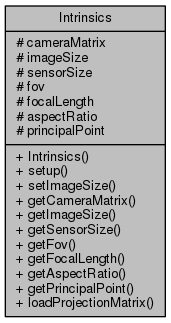
\includegraphics[width=0.3\textwidth]{class_intrinsics__coll__graph.png}
%  \caption{Clase Intrinsics}
%  \label{fig:classIntrinsics}
%\end{figure}
La clase \texttt{Intrinsics} almacena la geometría y las características internas de la cámara. La matriz intrínseca o matriz de la cámara se representa como un objeto matriz \texttt{cv::Mat} de dimensiones 3x3 formada por los siguientes parámetros:

\begin{equation}
cameraMatrix=
\begin{bmatrix}
f_{x} & \gamma & c_{x} \\
0    & f_{y}   & c_{y} \\
0    & 0      & 1
\end{bmatrix}
\end{equation}

Los parámetros $f_{x}$ y $f_{y}$ representan la distancia focal en términos de distancia. $\gamma$ representa el coeficiente de asimetría entre los ejes $X$ e $Y$, pero por simplificar el modelo, tomaremos que tiene valor 0. Finalmente, $c_{x}$ y $c_{y}$ representan las coordenadas en píxeles del punto principal, que sería idealmente en el centro de la imagen.

A partir de la matriz de la cámara y el tamaño de la imagen capturada, la clase \texttt{Intrisics} calcula el resto de parámetros propios como son el campo visual \texttt{(fov)}, la distancia focal \texttt{(focalLength)}, el centro óptico \texttt{(principalPoint)} y la relación de aspecto \texttt{(aspectRatio)} mediante la función \texttt{cv::calibrationMatrixValues}. 

\begin{listing}[
  float=ht,
  language = C++,
  caption  = {Atributos de la clase Intrinsics},
  label    = code:Intrinsics]
 cv::Mat cameraMatrix;       // (fx 0 cx, 0 fy cy, 0 0 1)
 cv::Size imageSize;         // Size of the image
 cv::Size sensorSize;        // Size of the image
 cv::Point2d fov;            // Field of view
 double focalLength;         // Focal length
 double aspectRatio;         // Aspect Ratio
 cv::Point2d principalPoint; // Principal point (center)
\end{listing}

OpenGL asume que no existe distorsión en la cámara por lo que a la hora de calcular la matriz de proyección debemos tener en cuenta que los parámetros de la matriz de la cámara deben estar corregidos. De esta forma, se utilizaran dos instancias de la clase \texttt{Instrinsics}: \texttt{distortedIntrinsics} y \texttt{undistortedIntrinsics}. La primera instancia almacena los parámetros ``reales'' mientras que en \texttt{undistortedIntrinsics} se encuentran los parámetros corregidos mediante las funciones \texttt{cv::getOptimalNewCameraMatrix} y \texttt{cv::initUndistortRectifyMap}.

\begin{listing}[
  float=ht,
  language = C++,
  caption  = {Atributos de la clase Calibration},
  label    = code:Calibration]
  //Intrinsics
  Intrinsics distortedIntrinsics;
  Intrinsics undistortedIntrinsics;
  cv::Mat distCoeffs;
  
  // Calibration parameters
  vector<vector<cv::Point2f> > imagePoints;
  vector<vector<cv::Point3f> > objectPoints;
  float reprojectionError;
  vector<float> perViewErrors;
  vector<cv::Mat> boardRotations;
  vector<cv::Mat> boardTranslations;

  // Pattern Configuration
  CalibrationPattern patternType;
  cv::Size patternSize;
  cv::Size addedImageSize;
  cv::Size subpixelSize;
  float squareSize;
 
  // Auxiliar calibration variables
  cv::Mat grayMat;
  bool fillFrame;
  cv::Mat undistortBuffer;
  cv::Mat undistortMapX, undistortMapY;
  bool ready;
 \end{listing}

Aunque el proceso de calibrado para la cámara y el proyector sigue el mismo enfoque, hay ciertas particularidades propias de cada dispositivo en el proceso de calibrado. La clase \texttt{Calibration} implementa toda la funcionalidad común, que es la mayoría, mientras que se han definido las clases \texttt{CameraCalibration} y \texttt{ProjectorCalibration} que heredan de \texttt{Calibration} y terminan de definir los procesos específicos.

Finalmente la clase \texttt{CameraProjectorCalibration} encapsula un objeto de  \texttt{CameraCalibration} y otro de \texttt{ProjectorCalibration} con los parámetros intrínsecos de ambos dispositivos e incluye los vectores de rotación \texttt{(rotCamToProj)} y traslación \texttt{(transCamToProj)} que definen las transformaciones necesarias entre el sistema de referencia de la cámara y el sistema de referencia del proyector. 

\texttt{CalibrationCore} es la encargada de inicializar la calibración de calibrado mediante la configuración establecida y define el proceso a realizar en cada una de las fases que lo compone.  bucle Update/draw

La configuración del proceso:
\begin{listing}[
  float=ht,
  language = C++,
  caption  = {Configuración de la clase CalibrationCore},
  label    = code:CalibCore]
  // Threshold parameters
  circleDetectionThreshold = 160;
  
  // Application
  diffMinBetweenFrames = 4.0; 
  timeMinBetweenCaptures = 2.0; 
  
  //Boards parameters
  numBoardsFinalCamera = 20;  
  numBoardsFinalProjector = 20;
  numBoardsBeforeCleaning = 3;  
  numBoardsBeforeDynamicProjection = 5; 
  maxReprojErrorCamera = 0.20;
  maxReprojErrorProjectorStatic = 0.25;
  maxReprojErrorProjectorDynamic = 0.43;

  // Image Size
  projectorFrame.create(cv::Size(800,600), CV_8UC1);
  
  // --- INITIAL MODE ---
  setState(CAMERA); //CAMERA, PROJECTOR_STATIC, DEMO_AR
\end{listing}
  
\subsection{Calibración de la cámara}
En esta primera fase el objetivo es obtener los parámetros intrínsecos de la cámara. De forma continua, el sistema realiza capturas de imagen. Durante este proceso, se debe mostrar a la cámara el patrón impreso en distintas posiciones y orientaciones. 

Para cada imagen capturada, se realiza el siguiente proceso:

\begin{itemize}

\item Se realiza una \textbf{búsqueda de las esquinas de los cuadrados del patrón de calibración} en la imagen. Para detectar las esquinas se utiliza la función \texttt{cv::findChessboardCorners}. A esta función se le debe proporcionar la imagen actual donde buscar el patrón, las dimensiones del patrón y un vector de \texttt{cv::Point2f} donde se almacenaran los puntos de la imagen de las esquinas detectadas. Adicionalmente, para mejorar esta detección se emplea \texttt{cv::cornerSubPix}, que se encargará de ubicar estas esquinas en medidas de subpíxeles. Si se ha encontrado el tablero de ajedrez en la imagen, el vector de puntos devuelto se guardan en el vector \texttt{imagePoints} junto con las extracciones de los frames anteriores.  

\begin{listing}[
  float=ht,
  language = C++,
  caption  = {Detección de las esquinas del patrón \emph{Chessboard}},
  label    = code:findChessBoard]
  cout << "Detecting chessboard ...";
  found = cv::findChessboardCorners(currentFrame, patternSize, pointBuf, chessFlags);

  // improve corner accuracy
  if(found) {
    if(currentFrame.type() != CV_8UC1) 
    cv::cvtColor(currentFrame, grayMat, CV_RGB2GRAY);
    else 
    grayMat = currentFrame;
    
    if(refine)
    // the 11x11 dictates the smallest image space square size allowed
    // in other words, if your smallest square is 11x11 pixels, then set this to 11x11
    cv::cornerSubPix(grayMat, pointBuf, subpixelSize,  cv::Size(-1,-1), cv::TermCriteria(CV_TERMCRIT_EPS + CV_TERMCRIT_ITER, 30, 0.1 ));
  }
  
  imagePoints.push_back(pointBuf);
\end{listing}

\item \textbf{Se generan los puntos de las esquinas del patrón en el sistema de coordenadas globales} \texttt{(objectPoints)} correspondientes a la imagen actual, en funcion del tipo, dimensiones y el valor de la medida real del lado del cuadrado del patrón que se ha impreso a través de la función \texttt{updateObjectPoints}.
\begin{listing}[
  float=ht,
  language = C++,
  caption  = {Función \texttt{Calibration::updateObjectPoints()}},
  label    = code:updateObjectPoints]
  void Calibration::updateObjectPoints() {
    vector<cv::Point3f> points = createObjectPoints(patternSize, squareSize, patternType);
    objectPoints.resize(imagePoints.size(), points);
  }
\end{listing}

\item Para \textbf{realizar la asociación entre los puntos de la imagen y los del objeto} se utiliza la funcion \texttt{cv::calibrateCamera} que estima los parámetros intrínsecos y extrínsecos de la cámara para cada una de las vistas. Recibe los \texttt{objectPoints} y los \texttt{imagePoints } de todas las capturas que llevamos realizadas y el tamaño de la imagen capturada \texttt{(addedImageSize)}, y devuelve la matriz de la cámara \texttt{(cameraMatrix)}, los coeficientes de distorsión \texttt{(distCoeffs)} y un vector con los vectores de rotación \texttt{boardRotations} y traslación \texttt{boardTranslations} que se ha estimado para cada vista del patrón. Es decir, cada rotación del vector k-ésimo junto con el vector correspondiente k-ésimo de la traslación, convierte los puntos del patrón de calibración desde el sistema de coordenadas globales (en el que se especifican los puntos del objeto) al sistema de referencia de la cámara en la vista k-ésima. La función devuelve también el error de reproyección cometido para cada una de las vistas.

\begin{listing}[
  float=ht,
  language = C++,
  caption  = {Calibrado de la cámara mediante \texttt{cv::calibrateCamera} },
   label    = code:calibrateCamera]
   cv::Mat cameraMatrix = cv::Mat::eye(3, 3, CV_64F);
   distCoeffs = cv::Mat::zeros(8, 1, CV_64F);
   int calibFlags = 0;
   float rms = cv::calibrateCamera(objectPoints, imagePoints, addedImageSize, cameraMatrix, distCoeffs, boardRotations, boardTranslations, calibFlags);
   cout << "RMS reprojection error: " << rms << endl;
 \end{listing}

\item La función \texttt{cv::checkRange} \textbf{comprueba la integridad de los elementos de la matriz de la cámara y de los coeficientes de distorsión}, asegurando que son valores numéricos válidos. 

\item A partir de los parámetros intrínsecos obtenidos, se \textbf{actualiza el error de reproyección general} de la calibración \texttt{(updateReprojectionError())}, y se \textbf{calcula la matriz de proyección de la cámara corregida} \texttt{(undistortedIntrinsics)} aplicando los valores de distorsión.
  
\item Cada cierto número de iteraciones \textbf{se eliminan las calibraciones que tienen un error de reproyección mayor que el umbral definido} en la variable \texttt{maxReprojErrorCamera}
      
\begin{listing}[
  float=ht,
  language = C++,
  caption  = {Limpieza de calibraciones},
  label    = code:clean]  
void Calibration::clean(float maxReprojErrorCamera) {
  cout << "Cleaning ...";
   int removed = 0;
   for(int i = size() - 1; i >= 0; i--) {
     if(getReprojectionError(i) > maxReprojErrorCamera) {
       objectPoints.erase(objectPoints.begin() + i);
       imagePoints.erase(imagePoints.begin() + i);
       removed++;
     }
   }
   cout << "Done!" << endl;
   if(size() > 0 && removed > 0) 
   calibrate();
}
\end{listing}
 


\end{itemize}
      
Alcanzado el número de calibraciones correctas por debajo del error definido, se procede al \textbf{almacenamiento de los últimos parámetros calculados} en un fichero de tipo YAML. Para ello se usa un objeto de tipo \texttt{cv::FileStorage} para escribir el fichero \texttt{calibrationCamera.yml} con la estructura y formato definido.

\begin{listing}[
  float=ht,
  language = C++,
  caption  = {Almacenamiento de los parámetros intrínsecos en un fichero YAML},
  label    = code:FileStorage]
  void Calibration::save(string filename, bool absolute) const {
    if(!ready){
      cout << "Calibration::save() failed, because your calibration isn't ready yet!"<< endl;
    }
    cv::FileStorage fs(filename, cv::FileStorage::WRITE);
    cv::Size imageSize = distortedIntrinsics.getImageSize();
    cv::Size sensorSize = distortedIntrinsics.getSensorSize();
    cv::Mat cameraMatrix = distortedIntrinsics.getCameraMatrix();
    fs << "cameraMatrix" << cameraMatrix;
    fs << "imageSize_width" << imageSize.width;
    fs << "imageSize_height" << imageSize.height;
    fs << "sensorSize_width" << sensorSize.width;
    fs << "sensorSize_height" << sensorSize.height;
    fs << "distCoeffs" << distCoeffs;
    fs << "reprojectionError" << reprojectionError;
    fs << "features" << "[";
    for(int i = 0; i < (int)imagePoints.size(); i++) {
      fs << "[" << imagePoints[i] << "]";
    }
    fs << "]";
  }
\end{listing}

Una vez finalizada la calibración de la cámara, el sistema continua para obtener los parámetros intrínsecos del proyector.

\subsection{Calibración del proyector}
El cálculo de los parámetros intrínsecos de proyector se realiza mediante el mismo enfoque que en la cámara. Considerándolo como una \textit{«cámara inversa»} se puede aplicar el mismo modelo matemático de cámara \emph{pinhole}.

En esta fase, el sistema proyecta continuamente un patrón de círculos asimétricos con un tamaño y en una posición fija. El objetivo es que la cámara detecte el patrón y pueda establecer, una primera aproximación de la matriz de proyección del proyector. Posteriormente, estos parámetros serán refinados en la siguiente fase del proceso de calibrado, mediante la proyección del patrón dinámicamente.

En primer lugar, Se carga el fichero con los parámetros intrínsecos de la cámara y se establecen los puntos del patrón asimétrico en la imagen que se va a proyectar \texttt{(imagePoints)} y en el sistema de referencia global \texttt{(objectPoints)} utilizando parámetros y distancias fijas.  

\begin{listing}[
  float=ht,
  language = C++,
  caption  = {Inicialización de la fase de calibrado del proyector},
  label    = code:ProjectorStatic]
calibrationCamera.load("calibrationCamera.yml",false);
camProjCalib.resetBoards();
calibrationCamera.setupCandidateObjectPoints();
calibrationProjector.setStaticCandidateImagePoints();
\end{listing}

Se busca el patrón asimétrico en la imagen capturada, para ello se utiliza la funcion \texttt{cv::findCirclesGrid} que intenta determinar si la imagen de entrada contiene una cuadrícula de círculos. Si es así, la función localiza los centros de los círculos. Para la detección de los círculos esta función se apoya en un detector de regiones \emph{(Blob detector)} que configuramos mediante los siguiente parámetros para adaptar la búsqueda en función del tamaño de la imagen y el tamaño de las regiones que se van a detectar.

\begin{listing}[
  float=ht,
  language = C++,
  caption  = {Parametrización del \emph{Blob Detector}},
  label    = code:BlobDetector]
cv::SimpleBlobDetector::Params params;
params.minArea = 10;
params.minDistBetweenBlobs = 5;
cv::Ptr<cv::FeatureDetector> blobDetector = new cv::SimpleBlobDetector(params);
bool bProjectedPatternFound = cv::findCirclesGrid(processedImg, calibrationProjector.getPatternSize(), circlesImgPts, cv::CALIB_CB_ASYMMETRIC_GRID | cv::CALIB_CB_CLUSTERING, blobDetector);
\end{listing}

Se aplica una binarización de la imagen de entrada que permite la segmentación de los círculos proyectados y realizar una separación del patrón de tablero de ajedrez.

  
Encontrado el patrón de círculos, obtenemos los vectores de rotación \texttt{boardRot} y translación \texttt{boardTrans} de los puntos proyectados en el sistema de referencia de la cámara mediante la funcion \texttt{cv:solvePnP}


 Transform all image points to world points in camera reference frame  and then into the plane reference frame
Se transforman los punto de la imagen a puntos reales en el sistema de referencia de la cámara, y después al sistema de referencia del patrón
La cámara se utiliza para calcular la posición 3D de los círculos proyectados (por retroproyección) según el  sistema de coordenadas local de la cámara, y luego en el sistema de coordenadas local del patrón (que es el sistema de coordenadas "mundo"). Esto se hace en el método de "backProject" (método de la calibración clase, pero llama sólo cuando el objeto es de tipo "cámara"). 

Esto significa que podemos comenzar a computar los instrinsics del proyector porque tiene puntos 3d (los círculos proyectados) en coordenadas del mundo, y sus respectivos "proyección" "imagen" en el proyector plano. 

Para realizar la asociación entre los puntos de la imagen y los del objeto se utiliza la funcion \texttt{cv::calibrateCamera} que estima los parámetros intrínsecos y extrínsecos de la cámara para cada una de las vistas. Recibe los objectPoints y los imagePoints de todas las capturas que llevamos realizadas y el tamaño de la imagen \texttt{addedImageSize}. y devuelve la matriz de la cámara \texttt{cameraMatrix}, los coeficientes de distorsión {distCoeffs} y un vector con los vectores de rotación y traslación que se ha estimado para cada vista del patrón. Las funciones checkRange comprobar que cada elemento de la matriz de la cámara y de los coeficientes de distorsión es ni NaN ni infinito. Actualización de distortedIntrinsics, actualización del error de reproyección y calculo de undistortedIntrinsics:distortedIntrinsics.setup(cameraMatrix, addedImageSize);  updateReprojectionError();   updateUndistortion();

calibrationProjector.calibrate();

Se comprueba que el error de reproyección no es superior al umbral definido.

Este proceso se repite hasta capturar un número de patrones definido en la configuración. Una vez alcanzado el numero de patrones capturados y con un error inferior al umbral pasamos a la siguiente fase de calibrado.

\subsection{Calibración del sistema estéreo cámara-proyector}
En esta fase refinaremos la calibración de los parámetros intrínsecos del proyector calculados en la fase previa y realizaremos los cálculos para obtener los parámetros extrínsecos del sistema estéreo cámara-proyector.

A partir de ahora, generamos el patrón de círculos asimétricos de manera dinámica. A partir de la posición y las dimensiones del patrón de tablero de ajedrez observado por la cámara, con la función \texttt{setDynamicProjectorImagePoints} se calcula y genera un patrón de círculos asimétricos que se proyectará junto al de ajedrez. 

Dispondremos entonces de los puntos 3D en el sistema de referencia global (el patrón), que son los círculos proyectados, y también su proyección (puntos 2D en la imagen) en el sistema de referencia de la cámara y en el sistema de referencia del proyector. Esto significa que se puede utilizar  un procedimiento de calibración estéreo como el que proporciona OpenCV. 


Consideraremos en nuestro sistema estéreo que la posición y orientación relativa entre la cámara y el proyector es fija. En los paso previos, se ha  calculado la pose de un objeto respecto a la cámara $(R_1, T_1)$ y la pose para el mismo objeto pero respecto al proyector $(R_2, T_2)$, entonces esas poses se relacionan entre sí. Esto significa que, dado $(R_1,T_1)$, es posible calcular $(R_2,T_2)$ conociendo la posición y orientación de la segunda cámara con respecto a la primera cámara. Esto es lo que hace la función descrita. Calcula $(R,T)$ de modo que:

\begin{equation}
R_2 = R * R_1
T_2 = R * T_1 + T,
\end{equation}

Opcionalmente, se calcula la matriz esencial $E$:
\begin{equation}
E=\begin{bmatrix}
0 & -T_2 & -T_1\\ 
T_2 & 0  & -T_0\\ 
-T_1 & T_0 & 0 
\end{bmatrix} * R
\end{equation}

donde $t_i$ son componentes del vector de traslación $T: T = [T_0, T_1, T_2] ^ T$. Y la función también puede calcular la matriz $F$ fundamental:
\begin{equation}
F = cameraMatrix_2^ {-T} * E * cameraMatrix_1^{-1}
\end{equation}


Mediante la función \texttt{cv::stereoCalibrate} se estima la matriz de transformación entre dos cámaras que formen un par estéreo. En nuestro caso la cámara y el proyector. 

La funcion \texttt{cv::stereoCalibrate} también permite obtener los parámetros intrínsecos de cada dispositivo, sin embargo debido a la alta dimensionalidad del espacio de parámetros y el ruido que pueden introducir las imágenes de entrada, la funcion puede divergir de la solución correcta. Por tanto utilizaremos los parámetros intrínsecos calculados en las fases previas para cada uno de los dispositivos de forma individual, proporcionándolos a la funcion e indicándolo mediante el \emph{flag} CV\_CALIB\_FIX\_INTRINSIC. Esto acción, simplifica los cálculos que tiene que realizar la función y que se realicen cálculos erróneos de unas matrices de proyección que ya se han obtenido previamente con bastante precisión. 

Como hemos indicado, debemos proporcionar los puntos del patrón de calibración y las proyecciones de estos puntos observados respecto a la cámara y el proyector. \texttt{setDynamicProjectorImagePoints()} nos genera los puntos del patrón asimétrico y almacena la proyección de los puntos respecto de la cámara. La funcion \texttt{calibrationProjector.calibrate()} obtiene los parámetros intrínsecos y la proyección de los puntos del patrón respecto del proyector. 

Al estar diseñado el bucle del programa mediante un enfoque \emph{update/draw}, tenemos que proceder en dos iteraciones para dar tiempo a la imagen proyectada a refrescarse antes de tratar de detectarlo. De lo contrario podemos estar detectando el viejo patrón proyectado, pero el uso de los puntos de imagen más recientes (que rompe por completo la calibración por supuesto)

Con todos los parámetros necesarios calculados:
\begin{itemize}
  \item objectPoints: Puntos del patrón generado dinámicamente.
  \item auxImagePointsCamera: Proyecciones de los puntos del patrón desde el punto de vista de la cámara
  \item calibrationProjector.imagePoints: Proyecciones de los puntos del patrón desde el punto de vista del proyector
  \item cameraMatrix: Matriz de parámetros intrínsecos de la cámara
  \item cameraDistCoeffs: Coeficientes de distorsión de la cámara
  \item projectorMatrix: Matriz de parámetros intrínsecos del proyector
  \item projectorDistCoeffs: Coeficientes de distorsión del proyector
  \item calibrationCamera.getDistortedIntrinsics().getImageSize(): Tamaño de la imagen utilizada.
\end{itemize}  
 
\texttt{cv::stereoCalibrate} devuelve la matriz de rotación \texttt{rotation3x3}, el vector de translación \texttt{transCamToProj} entre el sistema de referencia de la cámara y el proyector y el error de reproyección obtenido. La función \texttt{cv::Rodrigues} transforma la matriz de rotación en el vector de rotación \texttt{rotCamToProj} que almacena el proceso de calibrado.

Cada cierto número de iteraciones, configurable en el sistema, se eliminan las capturas del patrón que el error de reproyección supere un determinado umbral. Y finalmente al alcanzar un numero suficiente de calibraciones correctas, se toman los valores de los parámetros intrínsecos y extrínsecos del proyector a los que converge el proceso como los finales, guardándolos en un fichero de tipo YAML al igual que se realizó con los parámetros intrínsecos de la cámara mediante un objeto de tipo cv::FileStorage. calibrationProjector.yml CameraProjectorExtrinsics.xml


Para finalizar, el sistema pasa al modo de validación del proceso de calibrado, donde de manera visual, comprobaremos la precisión de la calibración realizada.
  %setState(DEMO_AR);

\subsection{Verificación del proceso de calibrado}
Carga de los ficheros YAML y obtener instancias de los objetos:
%CameraCalibration calibrationCamera = camProjCalib.getCalibrationCamera();
%ProjectorCalibration calibrationProjector  = camProjCalib.getCalibrationProjector();

Se busca el patrón de tablero de ajedrez en la imagen y se extraen los puntos de las esquinas \texttt{chessImgPts}
%bool bPrintedPatternFound = calibrationCamera.findBoard(cameraFrame, chessImgPts, true);

Calcula los vectores de rotación \texttt{cv::Mat boardRot} y traslación \texttt{cv::Mat boardTrans} del patrón a la cámara
%calibrationCamera.computeCandidateBoardPose(chessImgPts, boardRot, boardTrans);

Seleccionamos los ObjectPoints correspondientes a las cuatro esquinas del patrón y se almacenan en \texttt{vector<cv::Point3f> auxObjectPoints}

%cv::Mat rotObjToProj, transObjToProj;

Componemos los vectores de rotación y traslación del objeto a la cámara con vectores cámara al projector para obtener las transformaciones objeto a proyector
%cv::composeRT(boardRot,  boardTrans,
%camProjCalib.getCamToProjRotation(), camProjCalib.getCamToProjTranslation(),
%rotObjToProj, transObjToProj);

Proyectamos con la funcion \texttt{cv::projectPoints} los puntos de las cuatro esquinas del patrón \texttt{auxObjectPoints}, mediante las transformaciones objeto-proyector y los parámetros intrínsecos del proyector

%projectPoints(cv::Mat(auxObjectPoints),
%rotObjToProj, transObjToProj,
%calibrationProjector.getDistortedIntrinsics().getCameraMatrix(),
%calibrationProjector.getDistCoeffs(),
%out);

Establecemos los puntos obtenidos en la proyección \texttt{vector<cv::Point2f> out} como la salida que tiene que representar el proyector y que deben coincidir físicamente si se ha realizado una buena calibración. calibrationProjector.setCandidateImagePoints(out);


\section{Tracking y registro}
El cálculo del registro requiere posicionar el sistema cámara-proyector, mediante su posición y
rotación, relativo a las hojas de papel que se encuentren en la escena capturada. Los métodos de
tracking, en general, son los encargados de obtener una estimación de la trayectoria que realiza un
objeto.

En GrayAR, se ha optado por implementar un sistema de tracking visual basado en una aproximación \textbf{\textit{bottom-up}}\cite{Marimon}, en la que se calculan los seis grados de libertad de la cámara a partir de lo que se está
percibiendo en la imagen.

%\begin{itemize}
%\item Una primera fase basada en una aproximación \textbf{\textit{bottom-up}}\cite{Marimon}, en la que se
%  calculan los seis grados de libertad de la cámara (ver sección Pose) a partir de lo que se está
%  percibiendo en la imagen.

%  \item En el caso de no poder determinar la \emph{pose} en la fase anterior, se realiza un enfoque
%  \textbf{\textit{top-down}}\cite{Marimon}, que estima la posición y rotación del papel en función de las
%  observaciones almacenadas en los estados anteriores.
%\end{itemize}


Conociendo las posiciones 2D de las aristas y vértices que definen la hoja de papel, y el modelo de
proyección de la cámara es posible estimar la posición y rotación 3D de la cámara relativamente al
documento. Aprovechando que conocemos la estructura de formato normalizado (según ISO 120/DIN 476) de una
hoja de papel, con un tamaño previamente conocido nos permite definir un sistema de coordenadas
local de cada hoja detectada, de modo que obtengamos la matriz de transformación 4x4 del sistema de
coordenadas de la hoja al sistema de coordenadas de la cámara.

El enfoque utilizado es similar al de ArUCo y ARToolkit, mediante un algoritmo de detección de bordes y un
método de estimación de la orientación. Sobre la imagen obtenida se inicia el primer paso de búsqueda de hojas de
papel. La imagen se convierte a blanco y negro para facilitar la detección de cuadriláteros;
primero se convierte a escala de grises, y después se binariza eligiendo un parámetro de
umbral “threshold” que elige a partir de qué valor de gris (de entre 256 valores distintos) se
considera blanco o negro. A continuación el algoritmo de visión por computador
extrae componentes conectados de la imagen previamente binarizada,cuya área es
suficientemente grande como para ser una hoja de papel. A estas regiones se les aplica un algoritmo
de detección de contornos, obteniendo a continuación los vértices y aristas que definen la
región de la hoja en 2D.

\subsection{Conversión a escala de grises (Grayscale)}
El primer paso en el proceso de detección consiste en convertir el frame capturado por la cámara a
escala de grises mediante la función \texttt{cv::cvtColor}. Esta función convierte una imagen de un
espacio de color a otro. La constante \texttt{CV\_BGR2GRAY} sirve para indicar que queremos pasar de
una imagen BGR (estándar de OpenCV) a otra en escala de grises.

\subsection{Umbralización o binarización (Thresholding)}
La umbralización consiste en definir un valor umbral y compararlo con cada uno de los píxeles de la
imagen. A los píxeles que estén por debajo del umbral se les asigna un valor, y a los que estén por
encima otro. De esta forma se divide toda la población de valores en tan sólo dos grupos, reduciendo
considerablemente la complejidad de la información a analizar.

En ARgos, se han desarrollado tres soluciones distintas para tratar de resolver este problema del
thresholding básico (fijo, adaptativo y el método Canny). En un principio, solo se implementaron
los métodos fijos y adaptativo, pero en una fase de optimización realizada posteriormente, se incluyo
el método Canny. Este algoritmo proporcionaba bordes más precisos, y es  tolerante a las
variaciones de iluminación, produciendo menores índices de ruido en la imagen binarizada.

\subsection{Extracción de contornos}
El siguiente paso del proceso es la detección de contornos, una operación un tanto distinta a las
anteriores por dos motivos principales. El primero es que no consiste en iterar aplicando una misma
función de forma monótona sobre todos los píxeles de la imagen. Y el segundo, es que el resultado que
se obtiene no es una nueva imagen, sino un colección de conjuntos de puntos sobre la imagen.

Para este paso se parte de la imagen resultante del paso anterior. Es decir, de una imagen que tan
solo consta de píxeles con valor cero o uno. Sobre ella se aplica un algoritmo que la barre,
empezando por su esquina superior izquierda, a la busca de un primer píxel a uno, y que cuando lo
encuentra es capaz de seguir la cadena de píxeles con valor uno que se encuentran unidos a él hasta
volver al píxel de partida. Esa cadena de píxeles a uno encontrados se denomina contorno. Y es más,
el algoritmo es capaz de encontrar todos los contornos presentes en la imagen, ya que cuando termina
con uno empieza de nuevo el proceso hasta asegurarse de haber barrido la imagen por completo.

El algoritmo es bastante potente, ya que no sólo es capaz de encontrar los contornos exteriores,
sino también los interiores a otros, y retornarlos clasificados jerárquicamente. ARgos utiliza la
función \texttt{cv::findContours} que implementa este algoritmo. En la documentación, así como la
referencia de implementación, se refiere al \textit{paper} original «Topological structural analysis
of digitized binary images by border following» de Satoshi Suzuki and Keiichi Abe.

Básicamente hay un contador de contornos encontrados y un buffer de píxeles recorridos. El contador
se inicializa a cero y el buffer con una copia de la imagen original. Se barre el buffer de arriba
abajo y de izquierda a derecha. Una transición de un píxel 0 a otro 1 indica que se ha detectado un
borde exterior, momento en que se suma uno al contador de contornos encontrados y se buscan todos
los píxeles 1 vecinos del encontrado. Si el píxel no tiene vecinos a 1 se cambia el valor del píxel
por el del contador con signo contrario y se empieza otra vez con el siguiente píxel. En caso
contrario se cambia el valor del píxel por el del contador, excepto que su valor sea mayor que 1, lo
que significa que ya ha sido visitado, y se continúa buscando vecinos a 1 hasta retornar al píxel
inicial. Una transición de un píxel con valor igual o mayor que 1 a otro 0 indica que se ha
detectado un borde interior, momento en que se repite el mismo proceso usado para los contornos
exteriores.

El algoritmo presenta una pequeña dificultad en los bordes de la imagen, y para solventarlo
presupone que la imagen está rodeada por los cuatro lados de píxeles con valor 0. Es decir, que el
buffer que utiliza tiene una fila más por encima y por debajo, y una columna más a derecha e
izquierda, que la imagen original.


\subsection{Aproximación a polígonos (Douglas-Peucker)}
Los contornos de los que se parte para este paso son colecciones de puntos. Todos y cada uno de los
píxeles que forman parte de ellos, ya que no se guardaron sólo las esquinas, sino cada píxel
individual encontrado. Esto permite tomar algunas decisiones tempranas, como por ejemplo descartar
los contornos que no tengan un mínimo de puntos. Es decir, aquellos que no son susceptibles de formar
la hoja de papel. ARgos descarta aquellos que no tengan un área delimitada entre 47000 y 49000
píxeles.

Sobre aquellos contornos que cumplan con la restricción de superficie, se calcula la envoltura
convexa del contorno. Matemáticamente se define la envoltura convexa de un conjunto de puntos $X$ de
dimensión $n$ como la intersección de todos los conjuntos convexos que contienen a $X$.

Dados $k$ puntos $x_1, x_2,\dots x_k$ su envoltura convexa $C$ viene dada por la expresión:
\begin{equation}
C(X) =\left\{\sum_{i=1}^k \alpha_i x_i \ \Bigg | \ x_i\in X, \, \alpha_i\in \mathbb{R}, \, \alpha_i \geq 0 \, , \sum_{i=1}^k \alpha_i=1\right\}
\end{equation}

Es decir, teniendo un conjunto de puntos en el plano, su envoltura convexa está definida por el
polígono convexo de área mínima que cubre todos los puntos (esto es, todos los puntos están dentro
del polígono). OpenCV proporciona la función \texttt{cv::convexHull} para encontrar la envoltura de
una conjunto de puntos 2D utilizando el algoritmo de Sklansky con una complejidad $O(N log N)$ en su
actual implementación.

El objetivo del cálculo de la envoltura es la de obtener un contorno \emph{limpio}, ya que tras este
paso se han eliminado puntos interiores debidos a reflejos, sombras o ruido en la imagen que se hubiesen
detectado. Otra ventaja, es que permite que existan pequeños solapamientos en los bordes, y aún así, se
siga detectando el contorno del papel.

GrayAR utiliza la función \texttt{cv::approxPolyDP}  para convertir una colección de puntos en un
polígono mediante el algoritmo de Douglas-Peucker. El algoritmo admite como entrada una lista de
puntos y una distancia máxima permitida. Define un segmento que va desde el primer punto de la lista
hasta el último, y calcula la distancia más corta que hay desde dicho segmento a todos y cada uno
del resto de puntos de la lista. Si encuentra un punto a una distancia mayor que la máxima pasada
como parámetro divide la lista y el segmento en dos, utilizando el punto encontrado como nuevo
extremo. Y vuelve a empezar el proceso comprobando cada nueva lista contra cada nuevo segmento de
forma individual, creando nuevas listas y segmentos si fuera necesario, de forma recursiva.

ARgos utiliza como distancia máxima para al algoritmo el 10\% del número de puntos que tiene cada
contorno de forma individual. Una vez convertidos los puntos a polígonos se descartan los que no
tengan cuatro lados.

En este punto, en los casos en los que no existan grandes solapamientos sobre el papel, debemos
obtener una serie de polígonos que se corresponden con las hojas detectadas en la imagen.

\subsection{Búsqueda de cuadriláteros en el espacio de Hough}
Mientras se este realizando alguna interacción con el documento, nuestra mano, dedos e incluso parte
del brazo estarán solapando gran parte de la hoja que queremos detectar. Tras aplicar el detector de
bordes a la imagen recibida, obtenemos segmentos no conectados que las funciones anteriores no serán
capaces de clasificar como cuadriláteros candidatos a ser una hoja de papel.

En estos casos, la búsqueda de la hoja de papel en la imagen se realiza mediante detectores de líneas basados
en la transformada de Hough.

La transformada de Hough es una técnica para detectar bordes llevando los puntos al espacio
paramétrico donde se transforman en rectas.
Basándose en lo anterior, la recta $y = m*x+n$ se puede representar como un punto $(m,n)$ en el
espacio de parámetros. Sin embargo, cuando se tienen rectas
verticales, los parámetros de la recta $(m,n)$  no están definidos. Por esta razón se utilizan los parámetros
que describen una recta en coordenada polares, denotados $(\rho,\theta)$.

El parámetro $\rho$ representa la distancia entre el origen de coordenadas y el punto$(x,y)$,
mientras que $\theta$ es el ángulo del vector director de la recta perpendicular a la recta original
y que pasa por el origen de coordenadas.

Usando esta parametrización, la ecuación de una recta se puede escribir de la siguiente forma:

\begin{equation}
y=(-\dfrac{\cos \theta}{\sin \theta}) * x + (\dfrac{\rho}{\sin \theta})
\end{equation}
que se puede reescribir como
\begin{equation}
\rho=x * \cos \theta + y * \sin \theta
\end{equation}

Entonces, es posible asociar a cada recta un par $(\rho,\theta)$ que es único si $\theta \in
[0,\pi)$ y $\rho \in \mathbb{R}$ ó $\theta \in [0,2\pi)$ y $\rho \geq 0$. El espacio
$(\rho,\theta)$ se denomina espacio de Hough para el conjunto de rectas en dos dimensiones.

Para un punto arbitrario en la imagen con coordenadas $(x_0,y_0)$, las rectas que pasan por ese punto
son los pares  $(\rho,\theta)$ con  $\rho=x*\cos \theta + y * \sin \theta$ donde $\rho$ (la
distancia entre la línea y el origen) está determinado por $\theta$. Esto corresponde a una curva
sinusoidal en el espacio  $(\rho,\theta)$, que es única para ese punto. Si las curvas
correspondientes  a dos puntos se intersecan, el punto de intersección en el espacio de Hough
corresponde  a una línea en el espacio de la imagen que pasa por estos dos puntos. Generalizando, un
conjunto de puntos que forman una recta, producirán sinusoides que se intersecan en los parámetros
de esa línea. Por tanto, el problema de detectar puntos colineales se puede convertir en un problema
de buscar curvas concurrentes.

Las zonas de este espacio donde más líneas se cortan se convierten en parámetros de posibles rectas
en el espacio de la imagen.

Se seleccionan un conjunto de las rectas detectadas para ser examinado en función de las siguientes características:

\begin{itemize}
\item El segmento se encuentra dentro o en la proximidades de la zona de proyección del
  sistema. Con esta restricción descartaremos aquellos segmentos que sabemos de antemano que no van
  a ser hojas de papel, como por ejemplo, otros objetos que se encuentren en la imagen o los bordes
  de la superficie donde se encuentra en prototipo.
\item El segmento es mayor que un valor umbral.
\item Sólo se tienen en cuenta los segmentos más próximos a los límites de proyección. El detector
  de Hough puede encontrar rectas en el interior de la hoja de papel que estamos buscando. Así solo
  seleccionaremos los posibles candidatos a formar el borde del papel.
\item Los ángulos que formen dos rectas contiguas estará comprendido dentro del rango de 75º a 105º.
\item Los ángulos que formen dos rectas opuestas deben ser cercanos a 180º ó 360º.
\end{itemize}

Tras la selección anterior obtendremos un conjunto de segmentos de rectas extraídas de la
imagen. Cuatro segmentos se consideran que formarán un cuadrilátero candidato si cumplen los
siguientes criterios:
\begin{itemize}
\item Las intersecciones de los cuatro segmentos están dentro de la imagen y próximos a la zona de
  proyección.
\item Sólo intersecan en cuatro puntos.
\item El área del cuadrilátero delimitado por las intersecciones esta entre 47000 y 49000 píxeles,
  ya que garantiza que el cuadrilátero que se detectó representa una hoja de papel.
\end{itemize}

Para ello se generan las posibles combinaciones de 4 segmentos del conjunto de rectas detectadas y
se analizan los criterios anteriores.

\subsection{Filtrado final}
Aún realizando todos estos descartes, ARgos incorpora un control adicional, ya que debido a que en
los pasos previos se detectan contornos tanto exteriores como interiores, puede ocurrir que se
detecten dos cuadriláteros, uno dentro de otro, siendo necesario descartar el más interno.
ARgos calcula la distancia media entre las esquinas de los polígonos y si encuentra dos que están
muy cerca descarta el de menor perímetro, que necesariamente será el más interno.

Por último, para el cálculo de las distancias entre esquinas es necesario un paso previo
en el que las esquinas tienen que estar ordenadas en el sentido contrario de las agujas del reloj
\textit{(anti-clockwise order)}.

\subsection{Cálculo de parámetros extrínsecos de la cámara}
Una vez detectadas e identificadas las hojas de papel de la imagen, se procede a calcular los parámetros extrínsecos de la cámara respecto a cada una de ellas. Para la mayoría de los cálculos basta con considerar a la lente como un agujero puntual a través del que pasa la luz a través de un centro de proyección común.

Essential problem in AR: POSE ESTIMATION
WHERE to put the CG object
ORIENTAION of CG object
SIZE of CG object

(translation)
(rotation)
(scaling)

Supongamos que se visualiza un objeto que se encuentra a una distancia $x_{1}$ de la lente, y que la
imagen proyectada por los rayos que salen de la lente se forma a una distancia $x_{2}$ tras la
lente. Se denomina disstancia focal a la relación que existe entre $x_{1}$ y $x_{2}$ :
\begin{equation}
\dfrac{1}{f} = \dfrac{1}{x_{1}} + \dfrac{1}{x_{2}}
\end{equation}

A la hora de representar los objetos del espacio observado (3D), se convierten a un plano de
visión (2D), y se tendrá que definir cual es la correspondencia entre las coordenadas del espacio y las de la representación. Para facilitar esta conversión, se utiliza el sistema de coordenadas \emph{«homogéneo»}. Este sistema de coordenadas tiene la particularidad de que permite pasar fácilmente coordenadas de un número de dimensiones a otro. Para ello, almacena las coordenadas con una dimensión adicional, de tal forma que para un espacio de 3D, utilizaríamos 4 coordenadas. El valor de la coordenada adicional indica entre otras cosas, si el punto se encuentra en el infinito, valor 0, o es un punto cualquiera, valor distinto de 0. En este sistema, si dos coordenadas son proporcionales, se refieren al mismo punto.

Las matrices de transformación, utilizadas para pasar de unas dimensiones a otras, suelen incluir 3 tipos de transformaciones: Rotación, Translación y eScalado. Podemos representarlas así:
\begin{equation}
  [R|t] = \begin{bmatrix} SR_{1,1} & SR_{1,2} & SR_{1,3} & T_{1}  \\
                          SR_{2,1} & SR_{2,2} & SR_{2,3} & T_{2}  \\
                          SR_{3,1} & SR_{3,2} & SR_{3,3} & T_{3}  \\
                             0    &     0    &     0    &  1
  \end{bmatrix}
\end{equation}

Para convertir las coordenadas del mundo a coordenadas de pantalla, de espacio tridimensional a bidimensional, los sistemas de visión artificial utilizan la siguiente fórmula:

\begin{equation}
q=MQ
\end{equation}
donde
\begin{equation}
  q=\begin{bmatrix} x \\ y \\ z \end{bmatrix} \quad M=\begin{bmatrix} f_{x} & 0 & c_{x} \\ 0 & f_{y} & c_{y} \\ 0 & 0 & 1 \end{bmatrix} \quad Q=\begin{bmatrix} X \\ Y \\ Z \end{bmatrix}
\end{equation}

Por tanto, $q$ representa el espacio bidimensional en coordenadas homogéneas, y $Q$ el espacio
tridimensional. $f_{x}$ es la distancia focal en el eje $X$, $f_{y}$ la distancia focal en el eje
$Y$, ($c_{x},c_{y}$) marcan el punto principal, el punto donde el eje de visión corta el plano de
visión (normalmente suele estar en el centro de la imagen, o muy cerca).

En ARgos se utiliza la función de OpenCV \texttt{cv::solvePnp}. Está, calcula la \emph{pose} (rotación y
traslación) de la hoja de papel, dado un conjunto de puntos del objeto \texttt{(ObjPoints)}, sus proyecciones en
la imagen correspondiente \texttt{(ImagePoints)}, así como la matriz de la cámara \texttt{(camMatrix)} y los coeficientes
de distorsión \texttt{(distCoeff)}. Esta función encuentra una \emph{pose} que minimiza el error de reproyección, es
decir, la suma de los cuadrados de las distancias entre las proyecciones \texttt{imagePoints} observados y
los \texttt{objectPoints} proyectados.

Se establece el centro del papel como centro de coordenadas $(0,0,0)$, por lo que las esquinas que se le proporcionan a la función son :
\begin{equation}
ObjPoints =\begin{bmatrix} -w/2 & -h/2 & 0 \\
                            w/2 & -h/2 & 0 \\
                            w/2 &  h/2 & 0 \\
                           -w/2 &  h/2 & 0
\end{bmatrix}
\end{equation}
Siendo $h$ y $w$ la altura y anchura de la hoja de papel respectivamente. Los ImagePoints corresponden a los píxeles que
representan las esquinas de la marca detectada, camMatrix son los parámetros intrínsecos de la
cámara y distCoeff, el vector de coeficientes de distorsión. Estos últimos parámetros se obtienen en
el proceso de calibración de la cámara y se mantienen fijos y conocidos durante todo el proceso.

\subsection{Refinamiento de la \emph{pose}}
El posicionamiento calculado puede variar en cada frame, aun cuando el papel no se haya movido
realmente. Esto puede ser debido a variaciones en la iluminación que alteran sensiblemente los
procesos de detección o errores debido a la naturaleza imprecisa de los métodos utilizados.

Este refinamiento de las percepciones se basa en la capacidad del sistema de almacenar las últimas
\textit{n} percepciones. Este parámetro es configurable en tiempo de compilación.


Cuando se recibe una última percepción, se calcula una media ponderada con las cuatro últimas
percepciones, de forma que la percepción refinada es la resultante de la siguiente fórmula:
\begin{equation}
P_{actual} = P_1*0.5 + P_2*0.25 + P_3*0.15 + P_4*0.1
\end{equation}

Siendo $P_1$ la percepción más reciente, y el resto las percepciones almacenadas en el histórico. De esta forma, se da más peso a la percepción más actual, pero se tiene en cuenta las anteriores. El resultado es un movimiento más fluido y suave, aunque da la sensación de haber un \textit{delay} al momento de representar la posición. Este retraso es lógico, al tener en cuenta percepciones pasadas.

%\subsection{Tracking mediante filtros de partículas}
%From the detection result, we have 2D positions of the four corners of the quadrangle. Since we are using a cardboard with known size, and the camera is calibrated, we can compute the relative rotation and translation of the camera to the cardboard. Then, our tracking state at frame k is represented by this relative pose in the following form
%\begin{equation}
%q_k = \left \lfloor r_x \quad r_y \quad  r_z \quad  t_x \quad  t_y \quad t_z  \right \rfloor
%\end{equation}

%Dónde $rx$, $ry$ y $rz$ son los ángulos de rotación a lo largo de los ejes $X$, $Y$, $Z$,
%respectivamente. $tx$, $ty$ y $tz$ son los ángulos traslación respectivamente a cada uno de sus ejes.

%El filtro de partículas se utiliza para estimar la densidad posterior de la pose de la cámara. La
%pose se representa como un conjunto de partículas discretas. Cada partícula tiene un peso para
%indicar el grado de confianza que representar la pose de la cámara.

%Los dos componentes principales de un filtro de partículas son el modelo dinámico del estado y el
%modelo de observación. El modelo dinámico estado determina cómo las partículas se propagan frame a
%frame. Es decir, la definición de la densidad $p(q_k|q_{k-1})$. El modelo de observación determina
%cómo se asignan pesos a las partículas que proporcionan la observación en ese marco. Que la
%observación en la trama actual sea $y_k$ y la secuencia de la observación hasta el fotograma actual
%$y_{1: k}$ , el filtro de partículas realiza el seguimiento de forma recursiva por la aproximación
%de la densidad posterior $p(q_k|y_{1:k})$. La salida del filtro de
%partículas es un conjunto de las muestras ponderadas $\left \{\left \{ q_k^1 \quad w_k^1 \right \},
%  \dots, \left \{ q_k^s \quad w_k^s  \right \}\right \}$ donde $S$ es
%el número de partículas. El diagrama de flujo del filtro de partículas utilizado en nuestro proyecto se muestra en la Figura 4.

%\subsubsection{Modelo dinámico de estado}
%Dado que la superficie cuadrangular está en movimiento libre, un modelo de paseo aleatorio simple
%basado en una densidad uniforme $U$ sobre el estado anterior [5] se utiliza. La variable e representa
%la incertidumbre sobre el movimiento del cuadrilátero detectado.

%\begin{equation}
%p(q_k|q_{k-1}) = U (q_{k-1} - e, q_{k-1} + e)
%\end{equation}

%\subsubsection{Modelo de observación}
%La observación en nuestro algoritmo es (18). Representa el mapa de características del segmento de
%línea obtenido de la trama de imagen actual.

%\begin{equation}
%y_k = L = \left \{l_1^k,l_2^k, \dots, l_m^k\right \}
%\end{equation}

%Para evaluar la probabilidad de cada partícula, lo primero que re-proyecto de las cuatro esquinas
%del cuadrilátero en el plano de la imagen de acuerdo con la postura representada por la
%partícula. Luego, se utiliza un algoritmo de coincidencia línea basado en distancias punto de línea
%y las diferencias angulares para encontrar las mejores líneas que coinciden con las cuatro líneas
%laterales del cuadrilátero en el marco actual. Entonces, si todas las líneas laterales del
%cuadrilátero representado por la partícula pueden igualar a un segmento de línea, podemos formar un
%cuadrilátero por los segmentos de línea coincidentes. Este patio se comprueba mediante los tres
%primeros criterios en el algoritmo de detección de cuadrilátero.

%Si cualquiera de las líneas laterales no pueden igualar a un segmento de línea en el mapa de entidad
%de línea o el cuadrángulo formado no puede pasar el procedimiento de comprobación, un peso muy
%pequeño se le asignará a la partícula. De lo contrario, la partícula puede igualar a un cuadrilátero
%real en la imagen actual. Para dar un resultado de seguimiento más preciso, se introdujo un esquema
%de reemplazo en nuestro modelo de observación. Para las partículas que pasan los criterios de
%coincidencia de línea y cuadrangulares procedimientos de comprobación, las cuatro líneas
%coincidentes forman un cuadrilátero real en la escena.

%A continuación, las cuatro esquinas del cuadrilátero se calculan a partir de las cuatro
%líneas. Estas esquinas entonces reemplazar los de la partícula. De esta manera, todas las partículas
%que sobreviven a partir de los procedimientos de evaluación representarán un cuadrilátero real en la
%escena. Desde las esquinas se calculan a partir de las líneas, la precisión de seguimiento puede
%estar en el nivel sub-píxel. La probabilidad se calcula entonces de acuerdo a la suma de los
%coeficientes de la superposición de:

%\begin{equation}
%p(y_k | q_k^n) = \sum_{t=1}^{4} r_{1}^t r_2^t
%\end{equation}

%Los pesos finales de las partículas se dan por la normalización de la suma de los pesos de 1:

%\begin{equation}
%w_k^n = \dfrac{p(y_k|q_k^n)}{\sum_{n=1}^{S} p(y_k|q_k^n)}
%\end{equation}


\section{Identificación de documentos}
EL objetivo de este módulo es la identificación rápida de documentos empleando algoritmos de
recuperación de imágenes, comparando el documento que está siendo analizado con una base de datos de
documentos conocidos por el sistema.

El prototipo construido ha sido configurado para funcionar con varios documentos proporcionados
por la asociación ASPRONA. Estos documentos son partes de trabajo reales que se utilizan en un
taller de serigrafía que tiene la asociación. Otra sugerencia realizada, y que han puesto de
manifiesto que sería de gran utilidad de cara una implantación real, es el reconocimiento de facturas.

Como ya se ha explicado en el capitulo del estado del arte, las técnicas para la identificación de
documentos se pueden dividir en dos categorías:

\begin{itemize}
\item Basados en la \textbf{búsqueda de coincidencias de características locales.}
\item Basados en \textbf{combinación coincidencias de características locales y la distribución del contenido} dentro de la página.
\end{itemize}

La solución implementada en ARgos, debido a los requerimientos anteriores, corresponde a la primera
de las técnicas. Es la más adecuada para la identificación de documentos estructurados o
semi-estructurados, como pueden ser el caso de formularios, facturas, billetes de tren o tickets.

A la hora de elegir entre los detectores basados en la extracción de características invariante que
dispone OpenCV, se ha preferido SURF frente otros descriptores como SIFT ó BRISK por las siguientes razones:

\begin{itemize}
\item \textbf{Velocidad de cálculo} considerablemente superior al resto de los detectores, sin ocasionar perdida del rendimiento.
\item \textbf{Más robusto} ante posibles transformaciones de la imagen.
\item \textbf{No necesita ningún paso previo de segmentación} y la identificación es para obtener documentos similares (no
idénticos) a la imagen utilizada como consulta.
\end{itemize}

A continuación se detallan los pasos que realiza el algoritmo.

\subsection{Eliminación de la transformación de perspectiva}
Este paso tiene como entrada la imagen en escala de grises obtenida
por la cámara y los cuadriláteros candidatos encontrados en el módulo
de detección de hojas de papel. Para cada hoja de papel, extrae la
región de la imagen que cubre cada una de ellas eliminando la
transformación de perspectiva, es decir, la deformación que se produce
en el papel debido a la perspectiva.

ARgos utiliza dos funciones de OpenCV para este paso:

\begin{itemize}
\item \textbf{\texttt{cv::getPerspectiveTransform}} calcula
  una matriz que multiplicada por un punto en el cuadrilátero origen
  devuelve un punto equivalente en el cuadrado destino.

\item \textbf{\texttt{cv::warpPerspective}} acepta una
  imagen, un cuadrilátero, una matriz de transformación, y retorna una
  nueva imagen del área cubierta por el cuadrilátero sobre la que se
  ha aplicado la matriz de transformación para eliminar la deformación
  debida a la perspectiva.
\end{itemize}

El resultado de este proceso es una imagen de cada una de las hojas de
papel encontradas. Una para cada cuadrilátero candidato. ARgos utiliza
un tamaño de 600x420 píxeles para las imágenes destino.

Aunque SURF es invariante a la rotación, translación y
escala, realizar este paso previo nos proporciona varias ventajas. Por
una lado, se puede realizar la identificación de varios documentos
dentro de la misma imagen, y al extraer de la imagen inicial el
documento a identificar, estamos eliminado \emph{ruido} que podría
influir en el resultado de la detección, aumentado la robustez del algoritmo mediante
el análisis exclusivo de la región a identificar dentro de la imagen
general.

\subsection{Extracción de Características}

El proceso de extracción consiste en la búsqueda de zonas en la imagen
con diferente apariencia que las que están a su alrededor, denominadas características \textit{(features)}. Normalmente las características suelen ser bordes, esquinas o zonas más brillantes u oscuras en
función del algoritmo utilizado en particular.

OpenCV proporciona la clase wrapper \textbf{FeatureDetector} con una interfaz común que permite
cambiar fácilmente entre diferentes algoritmos.


La función \textbf{detect} extrae los puntos clave de la imagen que
cumplan el umbral para el valor del determinante de la matriz
hessiana, definido en el constructor del extractor. Estos punto se
almacenan en una estructura tipo \textbf{\texttt{vector<cv::KeyPoint>}}.

\textbf{KeyPoint} es una clase genérica que ha sido diseñada para
almacenar puntos significativos (con la ubicación, orientación, escala
y alguna información adicional).

\subsection{Generación de Descriptores}
La clase \textbf{DescriptorExtractor} es la encargada de calcula
el vector que describe la característica de un punto significativo
para la posterior comparación entre otros puntos de interés. SURF
utiliza el histograma de gradientes, calculado a partir de la
cuantificación de los gradientes dentro de una área local. Una zona se divide
en subregiones y se calcula el histograma de gradiente en cada una de
ellas.

Mediante la función \textbf{compute} calcula los descriptores de los
puntos clave detectados en la imagen. Un descriptor se representa como
un vector de dimensión fija de un tipo básico. La mayoría de los
descriptores siguen este patrón, ya que simplifica el cálculo de las
distancias entre los descriptores. Por lo tanto, un conjunto de
descriptores se representa como un \textbf{\texttt{cv::Mat}}, donde cada fila
es un descriptor de un punto clave.

\subsection{Búsqueda de Coincidencias}
Para buscar una coincidencia entre varias imágenes, se extraen los
descriptores de la imagen de consulta y se accede a la estructura de
descriptores de las imágenes referencia con los
datos del vector de consulta calculado, devolviendo el vector almacenado más
similar.

Si el vector de consulta está vacío, significa que no se han podido
extraer descriptores del documento. En el sistema, esto ocurre
cuando se coloca la hoja por la parte posterior, que es totalmente
blanca y el extractor no puede encontrar puntos de referencia.

La implementación de la búsqueda se realiza mediante la clase
\textbf{DescriptorMatcher}. El buscador se configura para que utilice
la biblioteca FLANN (Fast Library for Approximate Nearest Neighbors)
que contiene una colección de algoritmos para la búsqueda rápida los
vecinos más cercanos en grandes conjuntos de datos.

El método de los k vecinos más cercanos \emph{(K-nn)}, es un clasificador
supervisado que calcula la probabilidad de que un elemento pertenezca
a una clase conocida.

Para su utilización en ARgos, se configura la clase \textbf{Flann}
con dos parámetros que especifican el algoritmo a utilizar y su parametrización.

\begin{itemize}
\item El primero es \textbf{IndexParams} donde se define el índice de búsqueda
que se construirá. Para SURF, se recomienda la utilización de árboles
k-dimensionales (kd-tree) aleatorios como estructuras de búsqueda, que
permiten realizar búsquedas en paralelo.

\item El segundo es \textbf{SearchParams}, en el que se indica el número de
veces que los árboles del índice deben ser recorridos de forma
recursiva. Valores altos dan mayor precisión, pero también conllevan
un mayor tiempo de procesado. Se utiliza el valor por defecto de 32.
\end{itemize}

Dos descriptores se consideran coincidentes si la distancia euclídea
entre ellos es baja. Para ello se incluye una condición de filtrado
basada en NNDR \emph{(Nearest Neighbor Distance Ratio)} con los resultados
del buscador FLANN para conseguir búsquedas más robustas y
precisas. Una coincidencia de descriptores se eliminará si la
distancia desde el descriptor de la consulta a su primer vecino más
cercano es mayor que un valor umbral, entre 0 y 1, multiplicado por la
distancia al segundo vecino más cercano. Este umbral, por lo general
se establece en 0,8 y obliga a que las coincidencias sean únicas. Este
requisito se puede hacer más estrictos, reduciendo del valor de este
umbral.

Finalmente, al comparar todas las imágenes almacenadas con la imagen
de referencia, la que mayor número de coincidencias haya obtenido, será
la candidata para devolver su índice como resultado de la identificación.


\section{Interfaz natural de usuario}

\emph{Interfaz natural de usuario} es un término genérico para una variedad de tecnologías que
permiten a los usuarios interactuar con los ordenadores en términos humanos. Algunas de
estas tecnologías son las basadas en visión por computador y que son
capaces desde interpretar expresiones naturales como gestos hasta proporcionar información contextual que se
proyecta dentro del campo de visión del usuario.

En ARgos se ha creado una interfaz de usuario basada en zonas de
resaltado y botones virtuales que son proyectados directamente sobre
el documento. El usuario podrá interactuar directamente en el espacio físico sin utilizar sistemas de mando o dispositivos de entrada tradicionales como sería un ratón,
teclado, etc. siendo sustituidos por funciones más naturales como el
uso de movimientos gestuales con las manos.

Se ha realizado la implementación del paradigma de superficie táctil interactiva,
ampliamente utilizada en los actuales dispositivos portátiles como
tablets o smartphones, en la que al pulsar con un dedo sobre la
pantalla, reaccione instantáneamente a las acciones del usuario.

Al disponer únicamente de la imagen obtenida por la cámara del
sistema, la detección de una pulsación se abstrae a la localización
del extremo del dedo índice dentro de una región de interés. Todo
ello, realizado mediante técnicas de visión por computador.

\subsection{Segmentación de la mano}
El objetivo de este paso es generar de una máscara que discrimine o
diferencie entre los píxeles de una imagen que corresponden al color
de la piel y los que no pertenecen. Con está mascara se puede identificar y extraer la mano que
aparezca en la imagen y que esté realizando alguna acción sobre el documento a tratar.


Aunque existan diferentes colores de piel, muchos estudios han
demostrado que la mayor diferencia se presenta en la intensidad y no
el su crominancia, por lo tanto en lugar de utilizar el espacio de
color RGB, se utilizará el  \textbf{espacio de color HSV} (Hue, Saturation,
Value), que es más adecuado se aproxima a la percepción humana.


Se utilizan los canales de color H y S (matiz y saturación) para
detectar la piel. En el canal H, la piel se compone de zonas pequeñas
(representadas en negro), y otras mayores (representadas en gris). En
primer lugar, se realiza una \textbf{ecualización del histograma} del canal H
para conseguir una distribución uniforme. Es decir, que exista el
mismo número de píxeles para cada nivel de gris del histograma de del
canal.

A continuación, se aplica una \textbf{erosión morfológica} al canal para reducir los
contornos y separar las zonas similares próximas, a la vez que se
eliminan las zonas más claras separadas y amplían los pequeños detalles
oscuros.

Las operaciones morfológicas, consisten en la alteración de los píxeles
de salida de una imagen dependiendo del valor del píxel de entrada y
una relación de vecindad definida por un elemento estructural. El
elemento estructural define el tamaño y la forma con la que se aplica
la operación. En ARgos se aplica un elemento en forma de elipse de
tamaño 7x7 píxeles.

Para finalizar el tratamiento previo, se aplica un \textbf{filtro bilateral}
tanto al canal H como al S. El filtra bilateral es una herramienta muy
útil en visión por computador ya que permite suavizar las zonas
homogéneas de una imagen manteniendo los bordes.

En este momento la imagen se encuentra preparada para seleccionar
píxeles perteneciente a la piel. Se unifican los tres canales y
seleccionamos los píxeles que se encuentren entre los umbrales
$0 < H < 25$ y $80 < S < 255$

Finalmente se realiza una \textbf{limpieza morfológica} mediante las operaciones de
apertura y cierre. La apertura suaviza los contornos, elimina pequeñas
protuberancias y elimina las conexiones más débiles. El cierre,
rellena vacíos en los contornos y elimina pequeños huecos en la
imagen.

El resultado de este tratamiento es una imagen en escala de grises,
donde las zonas más claras pertenecen a píxeles de piel y los
contornos negros son zonas indeterminadas. Estableciendo un umbral, se
seleccionan los píxeles candidatos y \textbf{se genera la máscara} que
corresponderá a la región ocupada por la mano en la imagen.

\subsection{Análisis de la imagen para la detección de la mano}
Una vez que disponemos en una imagen binaria la región de la mano,
se aplica un \textbf{detector de contornos} sobre la imagen. En caso de no ser
único, el contorno que mayor longitud tenga entre los encontrados, corresponderá
a la mano.

Según la disposición del prototipo en relación a posición de los
documentos (situado a la izquierda de los papeles), establecemos la restricción de que la mano aparecerá por
la parte derecha del documento para interactuar con los botones, que
también serán proyectados sobre la zona derecha del documento. Además,
para la simulación de la pulsación es necesario tener el dedo índice
extendido. Por tanto, el extremo del dedo índice corresponde con el
 \textbf{punto del contorno situado más a la izquierda} dentro de la
imagen. Seleccionando este punto podemos situar la zona de pulsación
dentro de la pantalla.

\subsection{Cálculo de un punto 3D a partir de un punto en la imagen}
La función anterior obtiene el punto del extremo del dedo índice en
coordenadas $(x,y)$ de la pantalla. Este dato no sirve para saber
donde está colocado el extremo del dedo en relación a las
dimensiones reales del papel.

La opción de calcularlo mediante proporcionalidad de los píxeles que
forman el papel y sus dimensiones no es válida, ya que la distorsión
de la perspectiva generaría un error muy grande.

Para solventar el problema utilizaremos los parámetros intrínsecos y
extrínsecos de la cámara calculados de antemano y partiendo de la
relación entre los puntos del mundo real y los de la cámara:

\begin{equation}
s \begin{bmatrix}
u\\
v\\
1
\end{bmatrix} = M(R\begin{bmatrix}
X\\
Y\\
Z_{const}
\end{bmatrix}+t)
\end{equation}
donde $M$ es la matriz de la cámara, $R$ la matriz de rotación, $t$ el
vector de rotación, y $s$ es el factor de escala de la homografía. $Zconst$ representa la altura
donde se están representado los componentes gráficos en relación al
papel, en ARgos es 0.

\begin{equation}
R^{-1} M^{-1} s \begin{bmatrix}
u\\
v\\
1
\end{bmatrix} = \begin{bmatrix}
X\\
Y\\
Z_{const}
\end{bmatrix} R^{-1}t
\end{equation}

Resolviendo la ecuación anterior sustituyendo los puntos $(x,y)$ de la
pantalla en $(u,v)$ para conseguir $s$, obtenemos el punto 3D relativo
al papel, es decir, situando el centro de coordenadas $(0,0,0)$ en el
centro de la hoja.



\section{Módulo de soporte y utilidades}
\subsection{Gestor de configuración}
Existen muchos parámetros configurables en GrayAR. En las primeras versiones del proyecto estos parámetros estaban implementados en variables dentro del programa y cada vez que era necesario modificar estos parámetros, por ejemplo para la realizacion de pruebas, era necesario recompilar el código. Para los archivos que se encuentran en la raspberry, el tiempo de compilación al modificar el valor de uno de esto parámetros podia incluso a tardar varios minutos. Otro problema que surgió al crecer el proyecto esra que estos parámetros estaban repartidos entre varios ficheros, lo que suponia tener que recordar donde estaba localizado cada parametro y el consecuente riesgo de dejarse alguno sin actualizar que invalidaria las pruebas realizadas.

Lo primero que se realizo fue sacar todos los parámetros configurables a un fichero \acs{XML} que es leido al inicio del programa permitiendo que todos los parámetros sean accesibles por cualquier módulo dentro del programa.

Las ventajas son apreciables a instante, el proceso de pruebas es mucho más rápido, ya que no es necesario volver a compilar cada vez que se realiza un cambio en la configuración. Todos los parámetros se encuentran en un único fichero, que al ser \acs{XML}, tiene una estructura clara y legible para las personas, y que permite una edicion y modificacion sencilla. Tambien permite tener varios ficheros con distintas configuraciones y que se cargue en el programa uno u otro en funcion de las necesidades del momento.
 
La necesidad es la de tener una clase centralizada y accesible desde cualquier parte del programa que sea capaz de leer un fichero de configuración en \acs{XML} y almacene aquellas variables parametrizables de

Para implementar el gestor de configuración se ha creado la clase  \texttt{ConfigManager}. Esta tiene la funcion  \texttt{loadConfiguration} a la que se le indica el fichero \acs{XML} con la configuración a cargar 

Se ha optado por seguir el principio de diseño \acs{KISS} que establece que la mayoría de sistemas funcionan mejor si se mantienen simplesen lugar de hacerlos complejos; por ello, la simplicidad debe ser mantenida como un objetivo clave del diseño, y cualquier complejidad innecesaria debe ser evitada. Las ventajas genéricas que ofrece un patrón Singleton frente a la implementación de un clase estática como puede ser que las funciones se puedan sobreescribir en las clases herederas, que la inicialización asincrona mientras que una clase estática generalmente se inicializa cuando se carga por primera vez o que el singleton pueda ser manejado polimorficamente sin forzar a los usuarios a asumir que solo existe una instancia, no suponen un mejora para la funcionalidad que necesitamos implementar. 

\subsection{Funciones de representación para depuración}
Aunque la creación de funciones para la representación gráfica están fuera del alcance de este proyecto, a la hora de probar y depurar los distintos algoritmos implementados resulta muy practico disponer de algunas funciones de dibujado ya implementadas para corregir errores y tener una vision preeliminar de como puede quedar finalmente.

A partir de las primitivas de dibujado que ofrece OpenCV se han implementado una serie de funciones para facilitar la representación de contornos, esquinas, y una vez obtenidos los parámetros extrínsecos de las cámara y el proyector, dibujado de ejes, cubos u ortoedros que permiten validar si los cálculos se han realizado correctamente.






\chapter{Resultados}
\label{chap:resultados}




\section{Arquitectura}
En este capítulo se mostrarán los resultados obtenidos al aplicar la metodología descrita en la sección  \ref{chap:método}: \nameref{chap:método}
En el capítulo actual se describe la arquitectura de la plataforma QuQuSI a través de un
enfoque top-down, comenzando con una descripción general, continuando con las decisiones
de diseño y terminando con los detalles de implementación. La plataforma QuQuSI es un
sistema distribuido formado por una serie de aplicaciones (Fig. 5.1):


\subsection{Descripción general}
\subsection{Módulo de captura}
El módulo de captura de vídeo se encarga de crear y proporcionar fuentes de vídeo de diversa naturaleza para dar soporte al submódulo de registro (ver Sección 5.5), y al submódulo de representación 2D (ver Sección 5.3.4).
Es capaz de dar soporte multicámara. Se pueden crear tantas fuentes de vídeo como se disponga en el sistema, y el submódulo de vídeo las clasificará como: 
\begin{itemize}
\item RaspiCam: es necesaria esta fuente de vídeo para ejecutar una aplicación Minerva. Realiza el registro de la realidad y se dibuja de fondo.
\item Cámara USB: no es necesario que exista ninguna. Sirven de soporte para realizar registro sobre ellas, pero a priori no se visualiza al usuario.
\end{itemize}

El submódulo de vídeo se implementa en dos componentes: el VideoFactory, que proporciona la interfaz de creación y gestión de fuentes de vídeo, y el VideoSource, que implementa una única fuente de vídeo basáda en la biblioteca de visión artificial OpenCV.

OpenCV utiliza la clase cv::VideoCapture como abstracción de las de fuentes de vídeo a las que da soporte.
Para la realización de este proyecto se ha compilado una versión de OpenCV con soporte de archivos de vídeo basado en FFMPEG y con soporte de dispositivos de vídeo basado en Video4Linux 2. Así, la idea inicial de utilizar OpenCV para encapsular el acceso a cualquier tipo de fuente de vídeo 
\subsubsection{Biblioteca RaspiCam}



\subsection{Módulo de calibración}
Como ya se explicó en el capitulo \ref{chap:antecedentes}, los objetivos de realizar el proceso de calibración son la estimación de los parámetros intrínsecos y extrínsecos de la cámara. Los parámetros intrínsecos se refieren a las características internas de la cámara, como por ejemplo, su distancia focal, distorsión, y el centro de la imagen. Los parámetros extrínsecos describen su posición y orientación dentro de un espacio de refencia. Conocer los parámetros intrínsecos es un primer paso esencial, ya que permite calcular la estructura de la escena en el espacio euclideo y elimina la distorsión de lentes, la cual afecta a la precisión.

Se ha creado como una utilidad a parte del proceso principal. Ya que una vez calibrado el sistema, se proporcionan unos ficheros XML con los parametros intrinsecos y extrinsecos que se cargan en el proyecto. Mientras que la cámara y el proyector mantengan su posición y rotacion entre ellos, no es necesario realizar una nueva calibración y es posible mover todo el sistema.

El proceso de calibrado de la cámara esta basado esencialmente por el enfoque de [Zhang, 1999]. Se utiliza un patron tipo tablero de ajedrez, en la que se alternan cuadrados blancos y negros, de dimensiones conocidas. El patron se imprime y se pega sobre una superficie plana rígida.

A continuación se obtiene una serie de imágenes en los que se encuentre visible el patrón, con distintas orientaciones y distancias de la cámara. 

Se realiza el cálculo de las homografías entre el patrón y sus imágenes. Estas transformaciones proyectivas 2D producen un sistema de ecuaciones lineales que al resolverse obtiene los parámetros de la cámara. Esta fase generalmente es seguida por una etapa de refinamiento no lineal, basado en la minimización del error total de reproyección.

En principio, cualquier objeto caracterizado apropiadamente podría ser utilizado para la calibración. Existen otros métodos que basan sus referencias en objetos tridimensionales (por ejemplo, una caja cubierta con marcadores).  
La pricipal ventaja de la utilización de patrones planos, y que ha sido decisiva en la decisión del algoritmo a utilizar, es que son mucho más fáciles de tratar; resulta mucho más complicada la construcción y distribución de objetos 3D precisos para realizar una calibración.

El módulo implementado está basado en una extensión que han realizado Alvaro Cassinelli y Niklas Bergström a partir de un complemento de calibración desarrollado por Kyle McDonald que es capaz de calibrar cámaras y proyectores, consigiendo parametros intrínsecos de ambos, además de los extrinsecos en cuestión de varios minutos 

Aunque la cámara y el proyector podrían ser calibrados de forma simultánea, es mejor comenzar primero por calibrar la cámara.

El proyector proyecta un patron de circulos asimetrico, primero en una posición fija. La cámara se utiliza para calcular la posición 3D de los círculos proyectados, primero según el sistema de coordenadas de la camara, y luego segun el sistema de coordenadas del patron proyectado. Con esto parametros se calculan los parametros instrinsecos del proyector porque tiene puntos 3D (los círculos proyectados) en coordenadas reales, y sus respectivas proyecciones en el plano de imagen del proyector. El procedimiento de cálculo de homografiás es el mismo que para las cámaras, ya que el modelo matématico del proyector, es el de una cámara invertida. 


(c) Finally, we can start computing the extrinsics of the camera-projector (because basically we have 3d points in "world coordinates" (the board), which are the projected circles, and also their projection (2d points) in the camera image and projector "image"). This means you can use the standard stereo calibration routine in openCV (this is done in the function. The reason why we compute FIRST the instrinsics of the projector is because the method stereoCalibrationCameraProjector will call the openCV stereo calibration function using "fixed intrinsics" to ensure better convergence of the algorithm (presumably better because if the camera is very well calibrated first, then the instrinsics of the projector should be good - probably better than if recomputed from all the 3d points and image points in camera and projector). 
3) Once we get a good enough reprojection error (for the projector), we can start moving the projected points around so as to better explore the space (and get better and more accurate calibration). In this phase, we can run openCV stereo calibration to obtain the camera-projector extrinsics and again, we don't need to recompute the instrinics of the projector. After a few cycles (and cleaning of bad "boards"), the process converges, data is saved and you can do AR. 




calibración de la cámara / proyector comienza: el proyector proyecta una rejilla de círculos (primero en una posición fija, a continuación, como la calibración logra cierta exactitud, la parrilla de salida siguiendo el patrón impreso). Este paso es el siguiente: (a) la cámara se utiliza para calcular la posición 3D de los círculos proyectados (por retroproyección) en la cámara de sistema de coordenadas, y luego en el "tablero" de coordenadas del sistema de coordenadas (o "mundo"). Esto se hace en el método de "backProject" (método de la calibración clase, pero llama sólo cuando el objeto es de tipo "cámara"). 

Una vez calibrada, esta se se utiliza para calcular la posición 3D de los círculos proyectados (por retroproyección) en la cámara de sistema de coordenadas, y luego en el "tablero" de coordenadas del sistema de coordenadas (o "mundo"). Esto se hace en el método de "backProject" (método de la calibración clase, pero llama sólo cuando el objeto es de tipo "cámara"). 

(b) Esto significa que podemos comenzar a computar los instrinsics del proyector porque tiene puntos 3d (los círculos proyectados) en coordenadas del mundo, y sus respectivos "proyección" "imagen" en el proyector plano. 

(c) Finalmente, podemos empezar a calcular los extrinsics de la cámara-proyector (porque básicamente tenemos puntos 3d en "coordenadas mundo" (la mesa), que son los círculos proyectados, y también su proyección (puntos 2d) en la cámara imagen y proyector "imagen"). Esto significa que puede utilizar la rutina de calibración estéreo estándar en OpenCV (esto se hace en la función. La razón por la cual se calcula en primer lugar el instrinsics del proyector se debe a que el método stereoCalibrationCameraProjector llamará a la función de calibración OpenCV estéreo utilizando "intrínsecos fijos" para asegurar mejor convergencia del algoritmo (presumiblemente mejor, porque si la cámara está muy bien calibrado en primer lugar, a continuación, los instrinsics del proyector debe ser bueno - probablemente mejor que si recalculado desde todos los puntos 3D y puntos de imagen en la cámara y el proyector). 

3) Una vez que tengamos una buena error reproyección suficiente (para el proyector), podemos empezar a mover los puntos proyectados en torno a fin de explorar mejor el espacio (y obtener una mejor y más precisa calibración). En esta fase, podemos ejecutar la calibración estéreo OpenCV para obtener los extrinsics cámara-proyector y otra vez, no necesitamos para volver a calcular los instrinics del proyector. Después de unos pocos ciclos (y limpieza de malas "tablas"), el proceso converge, los datos se guardan y se puede hacer AR. 





\subsubsection{Calibración de la cámara}

\subsubsection{Calibración del proyector}

A continuación, la cámara se utiliza para calcular la posición 3D de los círculos proyectados (por retroproyección). Entonces podemos empezar a calibrar el proyector. Una vez que tengamos una buena error reproyección suficiente (para el proyector), podemos empezar a mover los puntos proyectados en torno a fin de explorar mejor el espacio (y obtener una mejor y más precisa calibración). En esta fase, podemos ejecutar la calibración estéreo OpenCV para obtener los parametros extrinsecos cámara-proyector. Después de unos pocos ciclos (y limpieza de malas "tablas"), el proceso converge, los datos se guardan y se puede hacer AR (*) 

Básicamente, el procedimiento se divide en tres pasos: 

 Notes: In case of camera/projector calibration, we need to proceed in TWO PHASES to give time to the projected image to refresh before trying to detect it (in case of "dynamic projected pattern"). Otherwise we may be detecting the OLD projected pattern, but using the newer image points (which completely breaks the calibration of course)
                
PHASE 1 goal is just to set the projector image points to be projected, so the projector  will project something to be detected in the draw function. The first time, this is using the recorded pattern, but later (as the projector gets calibrated) we can use some arbitrary points "closer" to the printed pattern.

In this later case (dynamic pattern), if the printed pattern is not visible, then we won't go to phase 2. 
                

En caso de calibración de la cámara / proyector, tenemos que proceder en dos fases para dar tiempo a la imagen proyectada para refrescar antes de tratar de detectarlo (en caso de "patrón proyectado dinámica"). De lo contrario podemos estar detectando el viejo patrón proyectado, pero el uso de los puntos de imagen más recientes (que rompe por completo la calibración por supuesto) 

FASE 1 gol es sólo para establecer los puntos de la imagen del proyector para ser proyectados, por lo que el proyector proyectará algo para ser detectado en la función draw. La primera vez, esto es usar el patrón grabado, pero más tarde (ya que el proyector se calibra) podemos utilizar algunos puntos arbitrarios "más cerca" del patrón impreso.



El proceso de calibrado del proyector se divide en dos fases










el proyector proyecta una rejilla de círculos (primero en una posición fija, a continuación, como la calibración logra cierta exactitud, la parrilla de salida siguiendo el patrón impreso). Este paso es el siguiente: 

























El funcionamiento del algoritmo de calibración se basa en encontrar las esquinas de los
cuadrados en el patrón de calibración y realizar una asociación entre ellos. Además, habrá
que proporcionar un valor de la medida real del mundo. Se proporciona la medida del lado
de un cuadrado del tablero de ajedrez para ello y se utiliza un vector con la medida de las
esquinas partiendo de esta base.
Los puntos detectados en las imágenes se almacenan en un vector de objetos cv::Point2f.
Para el programa se utilizará una matriz que contendrá dos vectores, uno por cada conjunto
de puntos en una de las imágenes. Los puntos 3D que miden las distancias de las esquinas del
tablero en unidades del mundo se almacenan en un vector de objetos cv::Point3f.
Para detectar las esquinas en las imágenes se utiliza la función cv::findChessboardCor-
ners(...). Adicionalmente, para mejorar esta detección se emplea cv::cornerSubPix, que se
encargará de ubicar estas esquinas en medidas de subpíxels 1 .




We use a pattern of alternating black and white squares (see Figure 11-9),
which ensures that there is no bias toward one side or the other in measurement. Also,
the resulting grid corners lend themselves naturally to the subpixel localization func-
tion discussed in Chapter 10.
Given an image of a chessboard (or a person holding a chessboard, or any other scene
with a chessboard and a reasonably uncluttered background), you can use the OpenCV
function cvFindChessboardCorners() to locate the corners of the chessboard.


In this routine, the method of
calibration is to target the camera on a known structure that has many individual and
identifi able points. By viewing this structure from a variety of angles, it is possible to
then compute the (relative) location and orientation of the camera at the time of each
image as well as the intrinsic parameters of the camera (see Figure 11-9 in the “Chess-
boards” section). In order to provide multiple views, we rotate and translate the object,
so let’s pause to learn a little more about rotation and translation.

Imprimir un Select a pattern, download, and print
Mount the pattern onto a rigid flat surface
Take many pictures of the target at different orientations and distances
Download pictures to compute and select ones that are in focus



\subsubsection{Cálculo de las matrices de transformación camara-proyector}
\subsection{Módulo de tracking y registro}
\subsection{Módulo de detección de documentos}
\subsection{Módulo de interaccion natural}
\subsection{Módulo de soporte y utilidades}
\subsubsection{Gestor de configuración}
Existen muchos parametros configurables en GrayAR. En las primeras versiones del proyecto estos parametros estaban implementados en variables dentro del programa y cada vez que era necesario modificar estos parametros, por ejemplo para la realizacion de pruebas, era necesario recompilar el código. Para los archivos que se encuentran en la raspberry, el tiempo de compilación al modificar el valor de uno de esto parametros podia incluso a tardar varios minutos. Otro problema que surgió al crecer el proyecto esra que estos parametros estaban repartidos entre varios ficheros, lo que suponia tener que recordar donde estaba localizado cada parametro y el consecuente riesgo de dejarse alguno sin actualizar que invalidaria las pruebas realizadas.

Lo primero que se realizo fue sacar todos los parametros configurables a un fichero XML que es leido al inicio del programa permitiendo que todos los parametros sean accesibles por cualquier módulo dentro del programa.

Las ventajas son apreciables a instante, el proceso de pruebas es mucho más rápido, ya que no es necesario volver a compilar cada vez que se realiza un cambio en la configuración. Todos los parametros se encuentran en un único fichero, que al ser XML, tiene una estructura clara y legible para las personas, y que permite una edicion y modificacion sencilla. Tambien permite tener varios ficheros con distintas configuraciones y que se cargue en el programa uno u otro en funcion de las necesidades del momento.
 
La necesidad es la de tener una clase centralizada y accesible desde cualquier parte del programa que sea capaz de leer un fichero de configuración en XML y almacene aquellas variables parametrizables de

Para implementar el gestor de configuración se ha creado la clase ConfigManager. Esta tiene la funcion loadConfiguration a la que se le indica el fichero xml con la configuración a cargar 

Se ha optado por seguir el principio de diseño KISS que establece que la mayoría de sistemas funcionan mejor si se mantienen simplesen lugar de hacerlos complejos; por ello, la simplicidad debe ser mantenida como un objetivo clave del diseño, y cualquier complejidad innecesaria debe ser evitada. Las ventajas genéricas que ofrece un patron Singleton frente a la implementación de un clase estática como puede ser que las funciones se puedan sobreescribir en las clases herederas, que la inicialización asincrona mientras que una clase estática generalmente se inicializa cuando se carga por primera vez o que el singleton pueda ser manejado polimorficamente sin forzar a los usuarios a asumir que solo existe una instancia, no suponen un mejora para la funcionalidad que necesitamos implementar. 

\subsubsection{Funciones de representación para depuración}
Aunque la creación de funciones para la representación gráfica están fuera del alcance de este proyecto, a la hora de probar y depurar los distintos algoritmos implementados resulta muy practico disponer de algunas funciones de dibujado ya implementadas para corregir errores y tener una vision preeliminar de como puede quedar finalmente.

A partir de las primitivas de dibujado que ofrece OpenCV se han implementado una serie de funciones para facilitar la representación de contornos, esquinas, y una vez obtenidos los parametros extrinsecos de las camara y el proyector, dibujado de ejes, cubos o cajas 3D que permiten validar si los cálculos se han realizado correctamente.



\chapter{Conclusiones y propuestas}
\label{chap:conclusiones}
\drop{E}{n} este capítulo se realiza un análisis sobre los objetivos alcanzados durante el desarrollo del presente Trabajo Fin de Grado, aportando en cada caso, las ventajas que ha supuesto la utilización o la elección de una determinada implementación respecto a otras opciones disponibles. A continuación, se exponen nuevos puntos de vista, que se pueden tratar en futuros trabajos para mejora ó ampliación del sistema, indicando una posible implementación y una estimación del coste temporal en caso de realizarlos. 

\section{Objetivos alcanzados}

El objetivo principal de GrayAR es el desarrollo de los sistemas de captura, tracking, registro e identificación de documentos dentro del \textit{Proyecto ARgos}. Con tal fin, se ha construido un prototipo real basado en una Raspberry Pi, con una cámara de bajo coste y un proyector portátil, que montado sobre un trípode, muestra información visual alineada sobre un documento que se encuentre dentro de la zona de proyección. Para efectuar esta visualización, se tiene en cuenta el posicionamiento 3D relativo entre el documento y el sistema cámara-proyector, para que el registro de la amplificación visual sea perfecto.

Además, el sistema responde a distintas acciones que el usuario pueda efectuar sobre el espacio físico, ampliando la información relacionada que sea relevante a la acción realizada.

Por tanto, el objetivo principal queda satisfecho, como así ocurre también con aquellos objetivos específicos, definidos en el capítulo \ref{chap:objetivos} y detallada su solución entre los capítulos \ref{chap:metodo} y  \ref{chap:arquitectura}, que exponemos a continuación a modo de resumen.   

\begin{description}
\item[Captura y preprocesado de imágenes.] El sistema cuenta con un módulo capaz de obtener imágenes de los distintos tipos de cámaras que se le pueden acoplar, ofreciendo una interfaz común, a pesar de disponer de drivers y APIs diferentes. Se ha provisto de los filtros necesarios para el tratamiento de las imágenes, contando con funciones de escalado, umbralización, detección de bordes y detección de características.

Para el cálculo de los parámetros intrínsecos y extrínsecos tanto de la cámara como del proyector, se ha desarrollado una aplicación externa que permite un calibrado rápido y sencillo del sistema, mediante un patrón de tipo tablero de ajedrez, cada vez que sea necesario. Una vez realizada la calibración, obtenemos tres ficheros XML que son lo necesarios para poder realizar los cálculos de registro en el prototipo. 

\item[Sistema de identificación de documentos.] La identificación de documentos en GrayAR se ha realizado mediante un algoritmo de recuperación de imágenes basado en descriptores y comparará el documento que está siendo analizado con una base de datos de documentos conocidos por el sistema.

Estos documentos se proporcionan en el fichero de configuración, así como las acciones posibles que se pueden realizar sobre él. Este tipo de configuración permite un sistema adaptable y personalizable a cada organización y usuario. 

\item[Implementación de técnicas de tracking y registro.] Para conseguir una experiencia totalmente inmersiva, se han desarrollado técnicas de tracking y registro que permiten el cálculo de la \emph{pose} (rotación y translación del documento en el espacio 3D) en tiempo real. Esto nos permite, que podamos ofrecer al usuario la información proyectada sobre la hoja de papel, independiente de su posición, rotación o plano en el que se encuentre. Siempre y cuando, no se salga de los límites de la zona de proyección.

\item [Utilización de paradigmas de interacción natural con el usuario (NUI).] El usuario puede interactuar directamente en el espacio físico sin utilizar sistemas de mando tradicionales, como ratones o teclados. Sólo es necesario encender el prototipo, y según el usuario vaya colocando documentos, los desplace por la zona de proyección, realice interacciones señalándolo ó girándolo para mostrar la cara posterior, el sistema responderá automáticamente a la acción realizada. 

La respuesta se le ofrece al usuario amplificada de varias formas (visual y/o auditiva) y siempre adaptada a la escena que se esté produciendo en ese mismo instante.

\item[Facilitar la gestión documental a personas con necesidades especiales.] GrayAR proporciona toda la información necesaria al sistema de representación \textit{(BelfegAR)}, para que realice el dibujado de la información visual relevante al contexto directamente sobre el espacio del papel.

Para complementar a la representación visual, se ha añadido a la Raspberry Pi un amplificador de audio LM386 montado sobre una placa de test con un altavoz de 1W, que hace las funciones de «tarjeta de sonido», permitiendo la reproducción de avisos, alertas o lecturas de texto para aquellas personas que necesiten de amplificación auditiva para la utilización del sistema.
  
\item[Se debe basar en componentes de bajo coste.] Para la construcción del prototipo se han seleccionado aquellos componentes, que dentro de unas prestaciones mínimas requeridas, fuesen lo más económicos posibles. El coste final (ver Sección 4.4) es muy reducido respecto a otros sistemas que puedan realizan funciones parecidas. El proyector, la parte más cara del sistema con un valor de 350\euro, lo podemos considerar económico, teniendo en cuenta que el precio medio de otros modelos es de 1000\euro.

Respecto al software empleado, todos los recursos y bibliotecas utilizadas son de licencia libre, y por tanto no están sujetos a pagos de licencias. 

\item[Dispositivo multiplataforma (hardware y software)]
El desarrollo de GrayAR se ha realizado exclusivamente en C++, siguiendo el estándar C++11. Los fichero de configuración y de calibrado están en \acs{XML}. El uso de bibliotecas externas ha sido mínimo, eligiendo las que no poseían dependencias de terceros, y siempre con licencias libres multiplataforma. Estas decisiones garantizan la portabilidad del sistema, tanto hardware como software (sistemas operativos), en forma de paquete único.
\end{description}


\section{Propuestas de trabajo futuro}
El \textit{Proyecto ARgos} no ha finalizado aún. GrayAR comprende las funciones de realidad aumentada y visión por computador que se han construido hasta el día de hoy en el \textit{Proyecto ARgos}. Algunas de la propuestas aquí reflejadas serán desarrolladas en la versión final de \textit{ARgos} y servirán de contexto para la realización de la tesis del Máster en Tecnologías Informáticas Avanzadas prevista para en este curso académico. 

Debido a la construcción modular y desacoplada del sistema, las ampliaciones o mejoras aquí planteadas son de ámbito local y solo afectarán al subsistema o módulo referido, siendo transparente los cambios realizados para el resto de la aplicación.
 
\begin{description}
\item [Tracking mediante aproximaciones \emph{top-down}.] Estas técnicas se basan en la estimación mediante modelos de movimiento basados en filtros bayesianos para predecir la posición de la cámara. A partir de la posición obtenida, se buscan referencias en la imagen que puedan corregir y ajustar la predicción.

Los filtros bayesianos a utilizar pueden clasificarse en dos tipos. Aquellos que trabajan con modelos de movimiento gausianos, se denominan Filtros de Kalman, y los que, por las características del ruido no pueden ser modelados mediante modelos gausianos, y se implementan mejor mediante Filtros de Partículas.

Estos métodos proporcionan robustez al proceso de tracking, ya que permite seguir detectando la hoja de papel, aun cuando exista una gran oclusión de la misma. 

Para la implementación de esta mejora, habría que valorar, además, el tiempo para analizar ambos enfoques y determinar cual de ellos se adapta mejor a las características de su desplazamiento por la zona de proyección. 

\item [Detección de páginas de texto mediante LLAH o similares.] La implementación actual de detección de documentos en GrayAR está basado en la búsqueda de coincidencias de características locales, ya que estos métodos obtienen mayor precisión de acierto en la detección de documentos con información semiestructurada, como es el caso de facturas o formularios. 

Sería interesante, como ampliación al sistema de detección, que se pudiesen reconocer documentos con alto contenido textual sin una estructura predeterminada de antemano. Para ello, es necesario la implementación de algún algoritmo de detección basado en las características inherentes de la estructura del documento y el texto que contiene. 

LLAH \cite{Nakai} tiene una alta escalabilidad y el esquema de indexación y recuperación empleado es extremadamente rápido. Los autores han confirmado que LLAH tiene una tasa de acierto del 99\% y con un tiempo de procesamiento de 50 ms en una base de datos de 20 millones de páginas. 

Existen varias implementaciones optimizadas sobre LLAH para salvar las limitaciones iniciales del algoritmo. Sería un trabajo futuro la tarea de buscar sólo las publicaciones que se hayan hecho sobre LLAH e intentar crear una implementación conjunta con todas las optimizaciones.

%\subsection{Estimación inteligente de parámetros en algoritmos de filtrado según la iluminación existente}
%Los algoritmos de filtrado (suavizado de imágenes, detección de bordes,...) se definen a través de parámetros que determinan su comportamiento y el resultado de la imagen obtenida. Normalmente se determinan por decisión humana y permanecen estáticos durante toda la ejecución del programa. Elegidos en función de los mejores resultados obtenidos en unas circunstancias determinadas, las variaciones en la iluminación de la escena provocan que un parámetro que en un principio se pudo considerar óptimo, al instante no sea válido. También nos encontramos el caso de que exista un rango de valores que nos satisfagan.

%Se propone por tanto la creación de un sistema mediante técnicas de \textit{softcomputing} que analice la escena actual y determine qué valores son los más adecuados para obtener un resultado conocido o esperado, en una serie de filtros utilizados en GrayAR.

%Las ventajas de realizar esta implementación proporcionaría, que los métodos de detección fuesen más robustos y tolerantes a los cambios de iluminación que se puedan producir durante la utilización del sistema.    

\item[Calibrado del sistema cámara-proyector mediante luz estructurada.] Otra técnica para el calibrado de proyectores es el propuesto por Daniel Moreno y Gabriel Taubin, basado luz estructurada, en el paper \textbf{\textit{«Simple, Accurate, and Robust Projector-Camera Calibration»}}.

La implementación, consistiría en los siguientes pasos a realizar \cite{Moreno}:
\begin{itemize}
\item Detectar la localización de las esquinas de un patrón de tablero de ajedrez en cada una las orientaciones capturados.
\item Estimar los componentes de luz directa y global.
\item Decodificar los patrones de luz estructurada.
\item Calcula una homografía local para cada una de las esquinas del patrón detectado.
\item Trasladar las posiciones de las esquinas a coordenadas del proyector mediante homografías locales.
\item Obtener los parámetros intrínsecos de la cámara utilizando las posiciones de las esquinas en la imagen.
\item Obtener los parámetros intrínsecos del proyector con las posiciones trasladadas al sistema de referencia del proyector.
\item Ajustar los parámetros intrínseco de la cámara y el proyector y obtener los parámetros extrínsecos del sistema en conjunto.
\item Opcionalmente, se puede realizar una optimización conjunta de todos los parámetros (intrínsecos y extrínsecos).
\end{itemize}

Este método no requiere ningún equipamiento especial y, según sus autores, es más preciso que otras técnicas de calibrado, ya que utilizan el modelo pinhole completo con distorsión radial. 

En base a la experiencia en el desarrollo del proceso de calibrado en GrayAR, esta historia se podría plantear para realizarse en un sprint de 3 ó 4 semanas de duración.  

\item [Utilización de cámaras con sensor de profundidad.] Sustituyendo la cámara principal, por otra equipada con sensores de infrarrojos (\acs{IR}) capaces de medir la profundidad de la escena, obtendríamos una mayor precisión y la posibilidad de aumentar la variedad de gestos reconocidos. 

Por ejemplo, realizar la acción de click (o doble click) con los dedos sobre la superficie de la mesa, ó la simulación de una superficie multitáctil.

El coste temporal de esta propuesta puede ser mayor que las anteriores. Habría que estudiar las bibliotecas existentes para la utilización del dispositivo (por ejemplo, kinect), proporcionar un nuevo sistema de calibrado para la cámara IR, y también, seria necesaria la modificar los métodos de reconocimiento gestual, que tendrían un enfoque distinto, debido a la información adicional de la cámara de profundidad.
\end{description}



% Local Variables:
% coding: utf-8
% mode: latex
% mode: flyspell
% ispell-local-dictionary: "castellano8"
% End:

%\chapter{Conclusions and proposals}
\label{chap:conclusiones_eng}

\drop{I}{n} this chapter, we analyse the objectives that we have reached in the development of this end-of-degree project, providing in each case, the advantages that the use and choice of a specific implementation regarding to other available options have made. The following are different point of views which can be studied in future projects to improve or expand the system, indicating a possible implementation and an estimation of the temporary cost in case of developing the project.


\section{Achieved objectives}
The main objective of GrayAR is the development of capture, tracking and registration systems and the identification of documents that belong to the \textit{ARgos Project}. For this reason, a real prototype based on a Raspberry Pi board with ARM architecture, a low-cost camera and a portable projector has been built. It shows, mounting on a tripod, visual information aligned on a document which is in the projection area. To execute this visualisation, the main part is the relative 3D position between the document and the camera-projector system, in order to achieve a perfect visual amplification.

Moreover, the system responds to different actions that the user can do in the physical space, expanding information related to the desired action. 

Therefore, the main purpose is satisfied, as it occurs with the specific objectives, defined in chapter \ref{chap:objetivos_eng} and detailed their solution in chapters \ref{chap:metodo} and \ref{chap:arquitectura}. These are explained below as a synopsis.


\subsection{Image capture and processing}
The system is provided with a module that obtains different kind of attachable cameras, offering a common interface, despite of having different drivers and APIs. It has been provided with the required filters to process images, with scaling functions, thresholding, edge detection or characteristics detection. An external application has been developed to calculate the extrinsic and intrinsic parameters of both, camera and projector. This application allows a rapid and easy calibration of the system, using a checkerboard pattern, whenever it is needed. Once the calibration is done, we obtain three XML files, which are necessary to do the calculation of the registration in the prototype.

\subsection{System of document identification}
The identification of documents in GrayAR has been made by an image-retrieval algorithm based on descriptors and it will compare the document which is being analyzing with a document database, known for the system.

These documents are located in the configuration file, as well as the possible actions that can be made on it. This kind of configuration allows an adaptable and personalised system in each organisation and user.

\subsection{Implementation of tracking and registration techniques}
The tracking and registration module will have real-time pose calculation features (rotation and translation of the object in the 3D space) to reach a fully immersive experience. This can lead to offer the user the information projected on a sheet of paper, without a dependence of the position, rotation or plane in which is located, as long as it does not exceed the limits of the projection area. 


\subsection{Use of Natural User Interface (NUI) paradigms}
The user will directly interact with the physical space without using control systems or traditional input devices such as mouse, keyboard, etc. The only need is turning the prototype on and the system will automatically respond to the action that is done when the user places documents, moves them around the projection area or points or rotates them to show their back side.

The response is showed to the user amplified in different ways (visual and/or auditive), and it is always adapted to the scene that is happening at that moment. 


\subsection{Facilitation of document management for people with special needs using amplification of the information}
GrayAR will give all the required information to the representation system \textit{(BelfegAR)}, in order to draw the relevant visual information right on the paper area.

A LM386 audio amplification has been added to the Raspberry Pi to complement the visual representation. It has been built on a test board with a 1W loudspeaker, which has already «sound card» functions. It allows the reproduction of
warnings, alarms or reading of texts to those people who need the hearing amplification for the use of the system.

\subsection{It has to be based on low-cost components}
The selected components of the prototype structure have been chosen with a minimum price, but with a minimum required qualities as well. The final cost is very low compared to other systems that can execute similar functions.

The projector, which is the most expensive part of the system, costs 325\euro, and can beconsiderate an economic price, taking into account that the average price of other models is 1000\euro.

Regarding to the used software, every resource and library that have been used are freely licensed, and therefore, they are not subject to licence payment.

\subsection{Multi-platform device (hardware and software)}
The development of GrayAR has been exclusively done in C++, following the C++11 standard. The configuration and calibration files are done in XML. The use of external libraries has been minimised, choosing the ones that did not depend on third parties, and always having a multi-platform free licence. These decisions guarantee the system portability, as much hardware as software (operating systems), in a unique pack and integrated form.


\section{Proposals for a future project}
The \textit{ARgos Project} has not finished yet. GrayAR comprises the augmented reality and computer-based vision functions that have been developed until now in Argos project. Some of the proposals here reflected have been developed in the final version of Argos and will be the context to develop the thesis in the Advanced Information Technologies Masters, planned for the next academic year. 

Due to the modular and disconnected construction of the system, the extensions and improvements that are reflected here are local and they will only concern to the subsystem or the referred module, with transparent changes for the
rest of the application.

%\subsection{Expansion of the recognised gestures catalogue}
%In order to get an optimum user experience, it is necessary to have a wide
%range of actions that the user can do to interact with the system. ...

\subsection{Tracking with top-down approximation}
These techniques are based on the approximation of movement models based on Bayesian filters to predict the position of the camera. From this position, references are searched on the image to correct and adjust the prediction. 

The Bayesian filters that have been used can be classified into two types. One of them works with Gaussian movement models and are called Kalman Filters, the others cannot be model with Gaussian models because of the noise/interference
characteristics and are implemented better with Particle Filters.

These methods provide robustness/strength to the tracking process, considering that they let the sheet of paper be still detectable, even when there is abig occlusion of this. The time to analyse both focuses and determine which one is
better for the characteristics of its movement around the projection area should be valued to implement this improvement.

\subsection{Text pages detection using LLAH or similar}
The current implementation of documents detection in GrayAR is based on the search for the coincidences in the local characteristics, since these methods are precisely correct on the detection of documents with a semi-structured information, such as receipts and forms.

It would be interesting, as an extension of the detection system, to be able to recognise documents with a high textual content without a predetermined structure as a first sight. For this, it is necessary to implementate a detection algorithm based on the inherent characteristics of the structure of the document and the text that this one has.

LLAH~\cite{Nakai} has a high scalability and its indexing and recovery/reclamation scheme is extremely fast. The authors have confirmed that LLAH has achieved a hit rate of 99 percent and it has a processing time of 50 ms more in a database with more than 20 million of pages. 

Several optimized implementations about LLAH exist to overcome the initial limitations in the algorithm. The task of looking for the exclusive publications about LLAH could be a future project, and it would be interesting to create a coordinated implementation with all the optimizations.

\subsection{Smart estimation of parameters in filtering algorithms according to the existing illumination}
The filtering algorithms (image smoothing, edge detection...) are defined by parameters that determine its behaviour and the result of the obtained image. Usually, they are defined by human decision and they stay static for the whole execution of the programme. They are chosen depending upon the best results in certain circumstances, the variations in the lighting of the scene can cause that an acceptable parameter, considered optimum at first, changes its status and stops being acceptable. Furthermore, there is the case that a range of values that are not acceptable exits. 

Therefore, it is proposed the creation of a system with \textit{softcomputing} techniques, which analyses the current scene and determines which values are the most appropriate to obtain a known or expected result, in a series of filters used in GrayAR. 

The advantages of doing this implementation would provide more robust/stronger detection methods and toleration to the light changes that can be produced while the system is being used.

\subsection{Calibration of the camera-projector system using structured light}
Another technique for the calibration of projectors is the technique proposed by Daniel Moreno and Gabriel Taubin, based on structured light, in the paper called \textbf{\textit{«Simple, Accurate, and Robust Projector-Camera Calibration»}}. 

The implementation would consist of the following steps to perform \cite{Moreno}:

\begin{itemize}
\item Detect checkerboard corner locations for each plane orientation.
\item Estimate global and direct light components.
\item Decode structured-light patterns.
\item Compute a local homography for each checkerboard corner.
\item Translate corner locations into projector coordinates using local homographies.
\item Calibrate camera intrinsics using image corner locations.
\item Calibrate projector intrinsics using projector corner locations.
\item Fix projector and camera intrinsics and calibrate system extrinsic parameters.
\item Optionally, all the parameters, intrinsic and extrinsic, can be optimized together.
\end{itemize}

This method does not require any special equipment and, according to their authors, is more precise than other calibration techniques, considering that they use the complete pinhole model with radial distortion.
 
On the basis of the experience in the development of the calibration process in GrayAR, this issue could be carried out in a three-or-four-weeks sprint.

\subsection{Use of cameras with depth sensor}
Replacing the main camera with other equipped one with sensors IR capable of measure the depth of the scene, we would obtain a higher precision and the possibility of enlarge the variety of recognized gestures. For example, the execution of the click (or double click) action with the fingers over the table surface or the simulation of a multi-touch surface.

The temporary cost of this proposal could be higher than the previous ones, since we should study the existing libraries for the execution of the device (e.g. kinect) and provide a new calibration system for the IR camera. The modification of the gesture recognition methods would be necessary as well, and they would have a different perspective due to the incorporation of additional information of the depth camera.

\appendix
\appendixtitle
\chapter{Manual de calibración}




El proceso de calibrado del sistema se ha creado como una utilidad independiente del sistema principal de ARgos. Una vez calibrado el sistema, la aplicación proporciona los ficheros XML, con los parametros intrinsecos y extrinsecos, que necesita ARgos para el calculo del registro..


El proceso de calibrado de la cámara esta basado esencialmente por el enfoque de [Zhang, 1999]. Se utiliza un patron tipo tablero de ajedrez, en la que se alternan cuadrados blancos y negros, de dimensiones conocidas. El patron se imprime y se pega sobre una superficie plana rígida. Se debe dejar una zona despejada a continuación del tablero de ajedrez, ya que en esta zona se proyectará el patrón que utiliza el proyector para su calibrado.  

A continuación, colocamos la superficie bajo la cámara, en distintas orientaciones y distancias, para obtener una serie de imágenes en los que se encuentre visible el patrón.

Cuando el proceso disponga de al menos 20 imagenes válidas, realizará los calculos para obtener los parametros instrinsecos de cámara y los grabará en el fichero \texttt{calibrationCamera.xml}

El siguiente paso consiste en calibrar el proyector. Se proyecta un patron de circulos asimetrico, primero en una posición fija. Colocar la superficie



 La cámara se utiliza para calcular la posición 3D de los círculos proyectados, primero según el sistema de coordenadas de la camara, y luego segun el sistema de coordenadas del patron proyectado. Con esto parametros se calculan los parametros instrinsecos del proyector porque tiene puntos 3D (los círculos proyectados) en coordenadas reales, y sus respectivas proyecciones en el plano de imagen del proyector. El procedimiento de cálculo de homografiás es el mismo que para las cámaras, ya que el modelo matématico del proyector, es el de una cámara invertida. 



Se realiza el cálculo de las homografías entre el patrón y sus imágenes. Estas transformaciones proyectivas 2D producen un sistema de ecuaciones lineales que al resolverse obtiene los parámetros de la cámara. Esta fase generalmente es seguida por una etapa de refinamiento no lineal, basado en la minimización del error total de reproyección.



Aunque la cámara y el proyector podrían ser calibrados de forma simultánea, es mejor comenzar primero por calibrar la cámara.





Mientras que la cámara y el proyector mantengan su posición y rotacion entre ellos, no es necesario realizar una nueva calibración y es posible mover todo el sistema.


En principio, cualquier objeto caracterizado apropiadamente podría ser utilizado para la calibración. Existen otros métodos que basan sus referencias en objetos tridimensionales (por ejemplo, una caja cubierta con marcadores).  
La pricipal ventaja de la utilización de patrones planos, y que ha sido decisiva en la decisión del algoritmo a utilizar, es que son mucho más fáciles de tratar; resulta mucho más complicada la construcción y distribución de objetos 3D precisos para realizar una calibración.

\blindtext

%\chapter{Especificación de Requisitos Software}

\section{Introducción}
El objetivo de este proyecto es construir un sistema de ayuda a la gestión de documental que permita el tratamiento directo sobre documentos físicos impresos mediante el
uso de técnicas de visión por computador, síntesis visual y auditiva y técnicas de realidad aumentada

\subsection{Identificación}
El sistema software considerado para el desarrollo de los objetivos se conoce como \textbf{ARgos}. Se trata de un proyecto experimental, por lo que el versionado se realizará según la siguiente nomenclatura:
\begin{description}
\item[\textit{mayor}] Se mantendrá a 0 durante toda la fase de desarrollo inicial, hasta que se libere la primera versión funcional completa.
\item[\textit{minor}] Se utilizarán números pares para versiones ``estables'' e impares para las ``inestables'' o en fase de pruebas y depuración.
\item[\textit{micro}] Para incluir correcciones de software que no impliquen grandes cambios.
\item[\textit{fase}] Para definir si la versión se encuentra en alguna fase de liberación como \textit{alpha}, \textit{beta} o \textit{Release Candidate (RC)}. 
\end{description}
 \subsection{Propósito y Audiencia}

El objetivo de este documento es recoger los requerimientos funcionales y técnicos que deben ser contemplados para la definición y desarrollo del proyecto ARgos. 

Los requisitos para el sistema serán proporcionados por Carlos González Morcillo, creador e investigador principal del proyecto; la cátedra Indra-UCLM y la fundación Adecco, como financiadores del proyecto y la asociación ASPRONA, que con su experiencia en la atención a personas con discapacidad, propondrán escenarios y funcionalidades que son de utilidad para este colectivo. 

El usuario final del sistema serán personas que necesiten soporte en la gestión documental debido a cualquier tipo de discapacidad.

\subsection{Definiciones, acrónimos y abreviaturas}

\begin{tabular}{|l|p{11cm}|}
  \hline
  \textbf{Término}      & \textbf{Definición} \\ \hline
  Realidad aumentada    & Visión directa o indirecta de un entorno físico del mundo real, cuyos elementos se combinan con elementos virtuales en tiempo real \\ \hline
  Visión por computador & Subcampo de la inteligencia artificial cuyo propósito procesar una escena o las características de una imagen                      \\ \hline
  Lectura fácil         & Elaboración de textos siguiendo pautas y directivas que facilitan la lectura y el entendimiento de los mismos                      \\ \hline
\end{tabular}

\subsection{Referencias}
Esta sección incluye una lista de citas bibliográficas de  los documentos a los que se hace referencia en el presente informe. En esta sección también incluiremos informes relacionados que forman parte de la documentación del proyecto y sean de utilidad como material de soporte a este documento.

\begin{itemize}
  \item \textbf{ Ref. 1:}  ARgos: Estado del Arte.pdf
\end{itemize}

\subsection{Organización del documento}
Este documento se ha estructurado según las indicaciones del estándar IEEE 830-1998 para especificación de requisitos de software y contiene las siguientes secciones:

\textbf{Sección 2.} Se describe el sistema en desarrollo desde un punto de vista holístico. Se definen funciones, características, limitaciones, supuestos, dependencias y requisitos generales desde una perspectiva general del sistema. 


\textbf{Sección 3.} Se describen los requisitos específicos del sistema que se están desarrollando. Se enumeran y describen interfaces, características y requisitos específicos en un grado suficiente para iniciar la elaboración de una solución arquitectónica del sistema propuesto.


\textbf{Sección 4.} Proporciona la información de trazabilidad de los requisitos del proyecto. Cada característica del sistema es indexada por el número de requisito y vinculada a su situación y pruebas. 

\textbf{Sección 5 y sucesivas.} Apéndices con información adicional utilizada para crear este documento.

\section{Descripción general}
\subsection{Perspectiva del producto}
El sistema final desarrollado será un producto independiente y autosuficiente. Cada uno de los subsistemas que lo componen, se encargarán de soportar y resolver las necesidades que existan. 

\subsection{Funcionalidad del Producto}
construcción de un sistema de ayuda a la gestión de documentos impresos mediante el uso de técnicas de visión por computador, síntesis visual y auditiva y técnicas de realidad
aumentada con los siguientes componentes funcionales:
\begin{itemize}
\item \textbf{Cámara USB:} El sistema emplea una cámara de bajo coste o webcam como entrada al módulo de visión por computador.
\item \textbf{Cañón de proyección:} Utilizaremos un cañón de proyección portátil para mostrar información visual directamente alineada sobre el documento del mundo físico. El sistema responderá a las peticiones que el usuario realice directamente sobre el espacio físico ampliando información relacionada que sea relevante a la acción que quiera realizar.
\item \textbf{Unidad de proceso:} La unidad de proceso se encargará de tomar como entrada las imágenes obtenidas por la cámara USB y generar la salida para el cañón de proyección. Esta salida deberá tener en cuenta el posicionamiento 3D relativo entre el documento y el cañón para que el registro de la amplificación visual sea perfecto. El documento podrá moverse dentro de una región del escritorio y la amplificación deberá quedar perfectamente alineada en el espacio físico. El sistema de cómputo además deberá generar información auditiva relevante al documento que está siendo tratado (por ejemplo, sintetizando voz o generando alertas sonoras), así como mostrar información adicional en una pantalla. Se utilizará un computador en placa Raspberry Pi con arquitectura ARM.
\end{itemize}

\subsection{Características de los usuarios}
El fin de esté proyecto es construir un sistema que permita la integración laboral a personas con discapacidad. El tipo de usuarios a los que está dirigido es por tanto personas dentro de un amplio espectro de discapacidades.
Se debe proporcionar soporte a usuarios con discapacidades sensoriales (visuales y auditivas) e intelectuales.  

\subsection{Restricciones}
Debido a las características del sistema se deben tener en cuenta las siguiente restricciones:
\begin{description}

\item[Funcional en dispositivos móviles] El prototipo final se construirá sobre un dispositivos con arquitectura ARM con limitaciones de tanto en capacidad de computo como memoria. El sistema deberá estar optimizado para este tipo de dispositivos, obteniendo una respuesta fluida y en tiempo real.   

\item[Se debe basar en componentes de bajo coste] Para facilitar la implantación real en el entorno de trabajo, deberá funcionar con componentes de bajo coste, incorporando mecanismos de corrección de distorsión y registro 3D totalmente software.
\end{description}
%\subsection{Suposiciones y dependencias}

%-------------------------------------------
\section{Requisitos específicos}
\subsection{Requisitos comunes de los interfaces}
\subsubsection{Interfaces Hardware}
\begin{itemize}
\item La implementación del sistema se realizará sobre una Raspberry Pi Modelo B de 512MB de RAM y arquitectura ARM 
\item La visualización será a través de un pico-proyector mediante conexión HDMI
\item El acceso al sistema y conexión a internet se establece por medio de cable ethernet durante el desarrollo y pruebas, siendo la conexión WiFi el tipo de conectividad final
\end{itemize}

\subsubsection{Interfaces Software }
Versión preliminar. No definido

\subsubsection{Interfaces de usuario}
Versión preliminar. No definido

\subsubsection{Interfaces de comunicación}
Versión preliminar. No definido

\subsection{Requisitos funcionales}
\subsection*{Definidos en la línea base del proyecto}
\subsubsection*{RF-001: Adquisición de imágenes mediante cámara USB}

\begin{tabular}{|l|l|p{10cm}|}
\hline
\textbf{RF-001}& \multicolumn{2}{l|}{\textbf{Adquisición de imágenes mediante cámara USB}}                                                       \\ \hline
\textbf{Versión}        & \multicolumn{2}{l|}{1.0 (03/02/2014)}                                                                                           \\ \hline
\textbf{Dependencias}   & \multicolumn{2}{l|}{No tiene}                                                                                                   \\ \hline
\textbf{Descripción}    & \multicolumn{2}{l|}{Se deben obtener imágenes mediante  una cámara USB}                                                         \\ \hline
\textbf{Comportamiento} & \multicolumn{1}{c|}{\textit{\textbf{Orden}}} & \multicolumn{1}{c|}{\textit{\textbf{Acción}}}                                    \\ \hline
                        & \multicolumn{1}{c|}{1}                       & Invocación a la cámara                                                           \\ \cline{2-3} 
                        & \multicolumn{1}{c|}{2}                       & Obtención del fotograma actual                                                   \\ \hline 
\textbf{Importancia}    & \multicolumn{2}{l|}{Esencial}                                                                                                   \\ \hline
\textbf{Prioridad}      & \multicolumn{2}{l|}{Alta}                                                                                                       \\ \hline
\textbf{Comentarios}    & \multicolumn{2}{l|}{}                                                                                                           \\ \hline
\end{tabular}

\subsubsection*{RF-002: Adquisición de imágenes mediante raspiCam}
\begin{tabular}{|l|l|p{10cm}|}
\hline
\textbf{RF-001}         & \multicolumn{2}{l|}{\textbf{Adquisición de imágenes mediante raspiCam}}                                                         \\ \hline
\textbf{Versión}        & \multicolumn{2}{l|}{1.0 (03/02/2014)}                                                                                           \\ \hline
\textbf{Dependencias}   & \multicolumn{2}{l|}{No tiene}                                                                                                   \\ \hline
\textbf{Descripción}    & \multicolumn{2}{l|}{Se deben obtener imágenes mediante raspiCam}                                                                \\ \hline
\textbf{Comportamiento} & \multicolumn{1}{c|}{\textit{\textbf{Orden}}} & \multicolumn{1}{c|}{\textit{\textbf{Acción}}}                                    \\ \hline
                        & \multicolumn{1}{c|}{1}                       & Invocación a la cámara                                                           \\ \cline{2-3} 
                        & \multicolumn{1}{c|}{2}                       & Obtención del fotograma actual                                                   \\ \hline 
\textbf{Importancia}    & \multicolumn{2}{l|}{Esencial}                                                                                                   \\ \hline
\textbf{Prioridad}      & \multicolumn{2}{l|}{Alta}                                                                                                       \\ \hline
\textbf{Comentarios}    & \multicolumn{2}{l|}{}                                                                                                           \\ \hline
\end{tabular}
\subsubsection*{RF-003: Sistema de calibrado de cámaras}
\begin{tabular}{|l|l|p{10cm}|}
\hline
\textbf{RF-003}        & \multicolumn{2}{l|}{\textbf{Sistema de calibrado de cámaras}}                                                                    \\ \hline
\textbf{Versión}        & \multicolumn{2}{l|}{1.0 (03/02/2014)}                                                                                           \\ \hline
\textbf{Dependencias}   & \multicolumn{2}{l|}{\begin{tabular}[l]{@{}l@{}}RF-001 Adquisición de imágenes mediante cámara USB\\ RF-002 Adquisición de imágenes mediante raspiCam\end{tabular}}              \\ \hline
\textbf{Descripción}    & \multicolumn{2}{l|}{El sistema debe proporcionar un método para el calibrado de las cámaras}                                    \\ \hline
\textbf{Comportamiento} & \multicolumn{1}{c|}{\textit{\textbf{Orden}}} & \multicolumn{1}{c|}{\textit{\textbf{Acción}}}                                    \\ \hline
                        & \multicolumn{1}{c|}{1}                       & Mediante un patrón de calibración se realizan varias tomas                       \\ \cline{2-3} 
                        & \multicolumn{1}{c|}{2}                       & Cálculo de parámetros intrínsecos de la cámara                                   \\ \cline{2-3} 
                        & \multicolumn{1}{c|}{3}                       & Cálculo de los coeficientes de distorsión                                        \\ \cline{2-3} 
                        & \multicolumn{1}{c|}{4}                       & Devolución de resultados mediante fichero XML                                    \\ \hline
\textbf{Importancia}    & \multicolumn{2}{l|}{Esencial}                                                                                                   \\ \hline
\textbf{Prioridad}      & \multicolumn{2}{l|}{Alta}                                                                                                       \\ \hline
\textbf{Comentarios}    & \multicolumn{2}{l|}{}                                                                                                           \\ \hline
\end{tabular}

\subsubsection*{RF-004: Sistema de calibrado de proyectores}
\begin{tabular}{|l|l|p{10cm}|}
\hline
\textbf{RF-003}        & \multicolumn{2}{l|}{\textbf{Sistema de calibrado de proyectores}}                                                                \\ \hline
\textbf{Versión}        & \multicolumn{2}{l|}{1.0 (03/02/2014)}                                                                                           \\ \hline
\textbf{Dependencias}   & \multicolumn{2}{l|}{\begin{tabular}[l]{@{}l@{}}RF-001 Adquisición de imágenes mediante cámara USB\\ RF-002 Adquisición de imágenes mediante raspiCam\end{tabular}}              \\ \hline
\textbf{Descripción}    & \multicolumn{2}{l|}{El sistema debe proporcionar un método para el calibrado de las cámaras}                                    \\ \hline
\textbf{Comportamiento} & \multicolumn{1}{c|}{\textit{\textbf{Orden}}} & \multicolumn{1}{c|}{\textit{\textbf{Acción}}}                                    \\ \hline
                        & \multicolumn{1}{c|}{1}                       & Se proyecta el patrón de calibración y la cámara realiza varias tomas            \\ \cline{2-3} 
                        & \multicolumn{1}{c|}{2}                       & Cálculo de parámetros intrínsecos del proyector                                  \\ \cline{2-3} 
                        & \multicolumn{1}{c|}{3}                       & Cálculo de los coeficientes de distorsión                                        \\ \cline{2-3} 
                        & \multicolumn{1}{c|}{4}                       & Devolución de resultados mediante fichero XML                                    \\ \hline
\textbf{Importancia}    & \multicolumn{2}{l|}{Esencial}                                                                                                   \\ \hline
\textbf{Prioridad}      & \multicolumn{2}{l|}{Alta}                                                                                                       \\ \hline
\textbf{Comentarios}    & \multicolumn{2}{l|}{}                                                                                                           \\ \hline
\end{tabular}

\subsubsection*{RF-005: Configuración del sistema mediante argumentos por terminal}
\begin{tabular}{|p{3cm}|p{11.5cm}|}
\hline
\textbf{RF-005}         & \textbf{Configuración del sistema mediante argumentos por terminal}                                       \\ \hline
\textbf{Versión}        & 1.0 (03/02/2014)                                                                                           \\ \hline
\textbf{Dependencias}   & No tiene                                                                                                   \\ \hline
\textbf{Descripción}    & Parametrizar la configuración completa del sistema mediante argumentos                                     \\ \hline
\textbf{Importancia}    & Deseable                                                                                                   \\ \hline
\textbf{Prioridad}      & Media                                                                                                      \\ \hline
\textbf{Comentarios}    &                                                                                                            \\ \hline
\end{tabular}

\subsubsection*{RF-006: Captura de imágenes a distintas resoluciones}
\begin{tabular}{|p{3cm}|p{11.5cm}|}
\hline
\textbf{RF-006}         & \textbf{Captura de imágenes a distintas resoluciones}                                                      \\ \hline
\textbf{Versión}        & 1.0 (03/02/2014)                                                                                           \\ \hline
\textbf{Dependencias}   & \begin{tabular}[l]{@{}l@{}}RF-001 Adquisición de imágenes mediante cámara USB\\ 
                                                     RF-002 Adquisición de imágenes mediante raspiCam \end{tabular}                  \\ \hline
\textbf{Descripción}    & En un momento determinado se debe realizar la captura en la mayor resolución posible                       \\ \hline
\textbf{Importancia}    & Deseable                                                                                                   \\ \hline
\textbf{Prioridad}      & Media                                                                                                      \\ \hline
\textbf{Comentarios}    &                                                                                                            \\ \hline
\end{tabular} 

\subsubsection*{RF-007: Utilización de un fichero de vídeo como fuente de entrada}
\begin{tabular}{|p{3cm}|p{11.5cm}|}
\hline
\textbf{RF-007}         & \textbf{Utilización de un fichero de vídeo como fuente de entrada}                                           \\ \hline
\textbf{Versión}        & 1.0 (03/02/2014)                                                                                             \\ \hline
\textbf{Dependencias}   & No tiene                                                                                                     \\ \hline
\textbf{Descripción}    & El sistema podrá obtener los frames de entrada a partir de un fichero de vídeo                               \\ \hline
\textbf{Importancia}    & Deseable                                                                                                     \\ \hline
\textbf{Prioridad}      & Media                                                                                                        \\ \hline
\textbf{Comentarios}    &                                                                                                              \\ \hline
\end{tabular}

\subsubsection*{RF-008: Grabación de vídeo}
\begin{tabular}{|p{3cm}|p{11.5cm}|}
\hline
\textbf{RF-008}         & \textbf{Grabación de vídeo}                                                                                \\ \hline
\textbf{Versión}        & 1.0 (03/02/2014)                                                                                           \\ \hline
\textbf{Dependencias}   & \begin{tabular}[l]{@{}l@{}}RF-001 Adquisición de imágenes mediante cámara USB\\ 
                                                     RF-002 Adquisición de imágenes mediante raspiCam \end{tabular}                  \\ \hline 
\textbf{Descripción}    & El sistema debe poder grabar en vídeo lo que se captura por la cámara                                      \\ \hline
\textbf{Importancia}    & Deseable                                                                                                   \\ \hline
\textbf{Prioridad}      & Media                                                                                                      \\ \hline
\textbf{Comentarios}    &                                                                                                            \\ \hline
\end{tabular}

\subsubsection*{RF-009: Sistema de cálculo de homografías}
\begin{tabular}{|p{3cm}|p{11.5cm}|}
\hline
\textbf{RF-009}         & \textbf{Sistema de cálculo de homografías}                                                                  \\ \hline
\textbf{Versión}        & 1.0 (03/02/2014)                                                                                            \\ \hline
\textbf{Dependencias}   & \begin{tabular}[l]{@{}l@{}}RF-001 Adquisición de imágenes mediante cámara USB\\ 
                                                     RF-002 Adquisición de imágenes mediante raspiCam \end{tabular}                   \\ \hline
\textbf{Descripción}    & Debe existir un módulo de cálculo de homografías para la correcta representación debido a la proyección de perspectiva en el proyector    \\ \hline 
\textbf{Importancia}    & Esencial                                                                                                    \\ \hline
\textbf{Prioridad}      & Alta                                                                                                        \\ \hline
\textbf{Comentarios}    &                                                                                                             \\ \hline
\end{tabular}

\subsubsection*{RF-010: Estimación de Pose 3D de documentos}
\begin{tabular}{|p{3cm}|p{11.5cm}|}
\hline
\textbf{RF-010}         & \textbf{Estimación de Pose 3D de documentos}                                                                \\ \hline
\textbf{Versión}        & 1.0 (03/02/2014)                                                                                            \\ \hline
\textbf{Dependencias}   & \begin{tabular}[l]{@{}l@{}}RF-002 Adquisición de imágenes mediante raspiCam\\ 
                                                     RF-003: Sistema de calibrado de cámaras\end{tabular}                             \\ \hline
\textbf{Descripción}    & Debe existir un módulo de cálculo estimación de la pose del documento en tiempo real                        \\ \hline 
\textbf{Importancia}    & Esencial                                                                                                    \\ \hline
\textbf{Prioridad}      & Alta                                                                                                        \\ \hline
\textbf{Comentarios}    &                                                                                                             \\ \hline
\end{tabular}

\subsubsection*{RF-011: Implementación de tracking visual}
\begin{tabular}{|p{3cm}|p{11.5cm}|}
\hline
\textbf{RF-011}         & \textbf{Implementación de tracking visual}                                                                 \\ \hline
\textbf{Versión}        & 1.0 (03/02/2014)                                                                                           \\ \hline
\textbf{Dependencias}   & \begin{tabular}[l]{@{}l@{}}RF-001 Adquisición de imágenes mediante cámara USB\\ 
                                                     RF-002 Adquisición de imágenes mediante raspiCam\end{tabular}                   \\ \hline
\textbf{Descripción}    & Sistema de tracking visual mediante Optical Flow u otras técnicas                                          \\ \hline 
\textbf{Importancia}    & Esencial                                                                                                   \\ \hline
\textbf{Prioridad}      & Alta                                                                                                       \\ \hline
\textbf{Comentarios}    &                                                                                                            \\ \hline
\end{tabular}

\subsubsection*{RF-012: Sistema de representación mediante OpenGL ES}
\begin{tabular}{|p{3cm}|p{11.5cm}|}
\hline
\textbf{RF-012}         & \textbf{Sistema de representación mediante OpenGL ES}                                                      \\ \hline
\textbf{Versión}        & 1.0 (03/02/2014)                                                                                           \\ \hline
\textbf{Dependencias}   & No tiene                                                                                                   \\ \hline
\textbf{Descripción}    & Sistema de representación 3D mediante OpenGL ES de polígonos y texto                                       \\ \hline 
\textbf{Importancia}    & Esencial                                                                                                   \\ \hline
\textbf{Prioridad}      & Alta                                                                                                       \\ \hline
\textbf{Comentarios}    &                                                                                                            \\ \hline
\end{tabular}

\subsubsection*{RF-013: Sistema de identificación rápida de documentos}
\begin{tabular}{|p{3cm}|p{11.5cm}|}
\hline
\textbf{RF-013}         & \textbf{Sistema de identificación rápida de documentos}                                                    \\ \hline
\textbf{Versión}        & 1.0 (03/02/2014)                                                                                           \\ \hline
\textbf{Dependencias}   & \begin{tabular}[l]{@{}l@{}}RF-001 Adquisición de imágenes mediante cámara USB\\ 
                                                     RF-002 Adquisición de imágenes mediante raspiCam\end{tabular}                   \\ \hline
\textbf{Descripción}    & El sistema debe poder identificar un documento capturado mediante la cámara  entre todos los almacenados en el sistema previamente  \\ \hline
\textbf{Importancia}    & Esencial                                                                                                   \\ \hline
\textbf{Prioridad}      & Alta                                                                                                       \\ \hline
\textbf{Comentarios}    &                                                                                                            \\ \hline
\end{tabular}

\subsubsection*{RF-014: Extracción de documentos digitales almacenados}
\begin{tabular}{|p{3cm}|p{11.5cm}|}
\hline
\textbf{RF-014}         & \textbf{Extracción de documentos digitales almacenados}                                                     \\ \hline
\textbf{Versión}        & 1.0 (03/02/2014)                                                                                            \\ \hline
\textbf{Dependencias}   & \begin{tabular}[l]{@{}l@{}}RF-001 Adquisición de imágenes mediante cámara USB\\
                                                     RF-002 Adquisición de imágenes mediante raspiCam\end{tabular}                    \\ \hline
\textbf{Descripción}    & El sistema debe poder devolver la versión digital del documento  identificado en  la fase anterior           \\ \hline
\textbf{Importancia}    & Esencial                                                                                                    \\ \hline
\textbf{Prioridad}      & Alta                                                                                                        \\ \hline
\textbf{Comentarios}    &                                                                                                             \\ \hline
\end{tabular}

\subsubsection*{RF-015: Interacción mediante paradigmas naturales con el usuario (NUI)}
\begin{tabular}{|p{3cm}|p{11.5cm}|}
\hline
\textbf{RF-015}         & \textbf{Interacción mediante paradigmas naturales con el usuario (NUI)}                                     \\ \hline
\textbf{Versión}        & 1.0 (03/02/2014)                                                                                            \\ \hline
\textbf{Dependencias}   & \begin{tabular}[l]{@{}l@{}}RF-001 Adquisición de imágenes mediante cámara USB\\ 
                                                     RF-002 Adquisición de imágenes mediante raspiCam\end{tabular}                    \\ \hline
\textbf{Descripción}    & La interacción con el sistema debe ser realizada mediante gestos realizados sobre el documento              \\ \hline
\textbf{Importancia}    & Esencial                                                                                                    \\ \hline
\textbf{Prioridad}      & Alta                                                                                                        \\ \hline
\textbf{Comentarios}    &                                                                                                             \\ \hline
\end{tabular}

\subsubsection*{RF-016: Amplificación multimodal}
\begin{tabular}{|l|l|p{8.5cm}|}
\hline
\textbf{RF-016}         & \multicolumn{2}{l|}{\textbf{Amplificación multimodal}}                                                                          \\ \hline
\textbf{Versión}        & \multicolumn{2}{l|}{1.0 (03/02/2014)}                                                                                           \\ \hline
\textbf{Dependencias}   & \multicolumn{2}{l|}{No tiene}                                                                                                   \\ \hline
\textbf{Descripción}    & \multicolumn{2}{p{11.5cm}|}{Contará con diferentes modos de amplificación de la información del mundo real}                     \\ \hline
\textbf{Comportamiento} & \multicolumn{1}{c|}{\textit{\textbf{Elementos}}} & \multicolumn{1}{c|}{\textit{\textbf{Acción}}}                                \\ \hline
                        & \multicolumn{1}{c|}{1}                       & La información visual se amplificará empleando el cañón de proyección            \\ \cline{2-3} 
                        & \multicolumn{1}{c|}{2}                       & El sistema generará información auditiva relevante a la operación realizada      \\ \cline{2-3} 
\textbf{Importancia}    & \multicolumn{2}{l|}{Esencial}                                                                                                   \\ \hline
\textbf{Prioridad}      & \multicolumn{2}{l|}{Alta}                                                                                                       \\ \hline
\textbf{Comentarios}    & \multicolumn{2}{l|}{}                                                                                                           \\ \hline
\end{tabular}
\subsubsection*{RF-017: Soporte de audio en streaming}
\begin{tabular}{|p{3cm}|p{11.5cm}|}
\hline
\textbf{RF-017}         & \textbf{Soporte de audio en streaming}                                                                     \\ \hline
\textbf{Versión}        & 1.0 (03/02/2014)                                                                                           \\ \hline
\textbf{Dependencias}   & No tiene                                                                                                   \\ \hline
\textbf{Descripción}    & El sistema tendrá la capacidad para reproducir audio en streaming                                          \\ \hline
\textbf{Importancia}    & Esencial                                                                                                   \\ \hline
\textbf{Prioridad}      & Alta                                                                                                       \\ \hline
\textbf{Comentarios}    &                                                                                                            \\ \hline
\end{tabular}

\subsubsection*{RF-018: Soporte de vídeo en streaming}
\begin{tabular}{|p{3cm}|p{11.5cm}|}
\hline
\textbf{RF-018}         & \textbf{Soporte de vídeo en streaming}                                                                     \\ \hline
\textbf{Versión}        & 1.0 (03/02/2014)                                                                                           \\ \hline
\textbf{Dependencias}   & No tiene                                                                                                   \\ \hline
\textbf{Descripción}    & El sistema tendrá la capacidad para reproducir vídeo en streaming                                          \\ \hline
\textbf{Importancia}    & Esencial                                                                                                   \\ \hline
\textbf{Prioridad}      & Alta                                                                                                       \\ \hline
\textbf{Comentarios}    &                                                                                                            \\ \hline
\end{tabular}

\bigskip
\subsection*{Definidos por ASPRONA}
\subsubsection*{RFa-001: Realización de Videoconferencias}
\begin{tabular}{|l|l|p{10cm}|}
\hline
\textbf{RFa-001}        & \multicolumn{2}{l|}{\textbf{Realización de Videoconferencias}}                                                                  \\ \hline
\textbf{Versión}        & \multicolumn{2}{l|}{1.0 (03/02/2014)}                                                                                           \\ \hline
\textbf{Dependencias}   & \multicolumn{2}{l|}{\begin{tabular}[c]{@{}c@{}}RF-017 Soporte de vídeo en streaming\\ 
                                                                         RF-018 soporte de audio en streaming\end{tabular}}                               \\ \hline
\textbf{Descripción}    & \multicolumn{2}{l|}{El sistema debe soportar la conexión por videoconferencia}                                                  \\ \hline
\textbf{Comportamiento} & \multicolumn{1}{c|}{\textit{\textbf{Orden}}} & \multicolumn{1}{c|}{\textit{\textbf{Acción}}}                                    \\ \hline
                        & \multicolumn{1}{c|}{1}                       & El usuario solicita la asistencia por videoconferencia                           \\ \cline{2-3} 
                        & \multicolumn{1}{c|}{2}                       & Se establece contacto con el personal de soporte                                 \\ \cline{2-3} 
                        & \multicolumn{1}{c|}{3}                       & Conversación                                                                     \\ \cline{2-3} 
                        & \multicolumn{1}{c|}{4}                       & Finalización de la  conexión                                                     \\ \hline
\textbf{Importancia}    & \multicolumn{2}{l|}{Esencial}                                                                                                   \\ \hline
\textbf{Prioridad}      & \multicolumn{2}{l|}{Alta}                                                                                                       \\ \hline
\textbf{Comentarios}    & \multicolumn{2}{l|}{}                                                                                                           \\ \hline
\end{tabular}

\subsubsection*{RFa-002: Mensajes en Lectura Fácil}
\begin{tabular}{|p{3cm}|p{11.5cm}|}
\hline
\textbf{RFa-002}        & \textbf{Mensajes en lectura fácil}                                                                         \\ \hline
\textbf{Versión}        & 1.0 (03/02/2014)                                                                                           \\ \hline
\textbf{Dependencias}   & No tiene                                                                                                   \\ \hline
\textbf{Descripción}    & Todos los textos y mensajes del sistema deben aparecer escritos en lectura fácil                           \\ \hline
\textbf{Importancia}    & Esencial                                                                                                   \\ \hline
\textbf{Prioridad}      & Alta                                                                                                       \\ \hline
\textbf{Comentarios}    &                                                                                                            \\ \hline
\end{tabular}

\subsubsection*{RFa-003: Soporte para completar partes de trabajo}
\begin{tabular}{|p{3cm}|p{11.5cm}|}
\hline
\textbf{RFa-003}        & \textbf{Soporte para completar partes de trabajo}                                                          \\ \hline
\textbf{Versión}        & 1.0 (03/02/2014)                                                                                           \\ \hline
\textbf{Dependencias}   & No tiene                                                                                                   \\ \hline
\textbf{Descripción}    & Debe proporcionar el soporte necesario para rellenar un formulario de un parte de trabajo                  \\ \hline
\textbf{Importancia}    & Deseable                                                                                                   \\ \hline
\textbf{Prioridad}      & Media                                                                                                      \\ \hline
\textbf{Comentarios}    &                                                                                                            \\ \hline
\end{tabular}

\subsubsection*{RFa-004: Soporte para completar formularios de protocolos de calidad}
\begin{tabular}{|p{3cm}|p{11.5cm}|}
\hline
\textbf{RFa-004}        & \textbf{Soporte para completar formularios de protocolos de calidad}                                       \\ \hline
\textbf{Versión}        & 1.0 (03/02/2014)                                                                                           \\ \hline
\textbf{Dependencias}   & No tiene                                                                                                   \\ \hline
\textbf{Descripción}    & El sistema debe proporcionar el soporte necesario para completar un informe de calidad                     \\ \hline
\textbf{Importancia}    & Deseable                                                                                                   \\ \hline
\textbf{Prioridad}      & Media                                                                                                      \\ \hline
\textbf{Comentarios}    &                                                                                                            \\ \hline
\end{tabular}

\subsubsection*{RFa-005: Guiado para clasificación y archivado de facturas}
\begin{tabular}{|p{3cm}|p{11.5cm}|}
\hline
\textbf{RFa-005}        & \textbf{Guiado para clasificación y archivado de facturas}                                                \\ \hline
\textbf{Versión}        & 1.0 (03/02/2014)                                                                                           \\ \hline
\textbf{Dependencias}   & No tiene                                                                                                   \\ \hline
\textbf{Descripción}    & El sistema debe proporcionar soporte para la tarea de clasificación y archivado de facturas                \\ \hline
\textbf{Importancia}    & Esencial                                                                                                   \\ \hline
\textbf{Prioridad}      & Alta                                                                                                       \\ \hline
\textbf{Comentarios}    &                                                                                                            \\ \hline
\end{tabular}

\subsubsection*{RFa-006: Entorno configurable por el usuario}
\begin{tabular}{|p{3cm}|p{11.5cm}|}
\hline
\textbf{RFa-006}        & \textbf{Entorno configurable}                                                                              \\ \hline
\textbf{Versión}        & 1.0 (03/02/2014)                                                                                           \\ \hline
\textbf{Dependencias}   & No tiene                                                                                                   \\ \hline
\textbf{Descripción}    & El sistema debe contar opción de personalización ``amigable'' para el usuario                              \\ \hline
\textbf{Importancia}    & Opcional                                                                                                   \\ \hline
\textbf{Prioridad}      & Baja                                                                                                       \\ \hline
\textbf{Comentarios}    &                                                                                                            \\ \hline
\end{tabular}


\subsection*{Definidos por Indra/Adecco}
\subsubsection*{RFi-001: Reconocimiento de Firmas}
\begin{tabular}{|p{3cm}|p{11.5cm}|}
\hline
\textbf{RFi-001}        & \textbf{Reconocimiento de Firmas}                                                                          \\ \hline
\textbf{Versión}        & 1.0 (03/02/2014)                                                                                           \\ \hline
\textbf{Dependencias}   & No tiene                                                                                                   \\ \hline
\textbf{Descripción}    & Debe reconocer una firma manuscrita entre un conjunto de firmas almacenadas previamente                    \\ \hline
\textbf{Importancia}    & Esencial                                                                                                   \\ \hline
\textbf{Prioridad}      & Alta                                                                                                       \\ \hline
\textbf{Comentarios}    &                                                                                                            \\ \hline
\end{tabular}


\subsection{Requisitos no funcionales}
\subsubsection{Requisitos de rendimiento}
El sistema debe funcionar de manera fluida y en tiempo real en dispositivos móviles basados en arquitectura ARM. Sólo existirá un único usuario del sistema simultáneamente y los documentos a tratar también se tratarán de uno en uno.
\subsubsection{Seguridad}
A parte de la información que se proporcione al usuario directamente, se mantendrá un log donde se registrará toda la actividad realizada en el sistema.
Debido al carácter experimental del proyecto, no se tendrán en cuenta la aplicación, por lo menos en la primera fases de desarrollo, de técnicas criptográficas para ficheros, bases de datos o comunicaciones.
\subsubsection{Fiabilidad}
Todo tipo de incidente producido en el sistema debe ser controlado y tratado. 
\subsubsection{Disponibilidad}
La disponibilidad del sistema debe ser de al menos un 99\% del tiempo que esté en ejecución. En caso de caída del sistema se deben proporcionar mecanismos automáticos para que la maquina y el sistema se reinicien y sean nuevamente operativos sin la necesidad de intervención directa del usuario,
\subsubsection{Mantenibilidad}
El desarrollo en un dispositivo tan reciente implica que se liberen con relativa frecuencia bibliotecas o controladores, en los que se corrigen bugs y/o mejoran su rendimiento. Seria recomendable hacer una revisión de los módulos actualizados antes de la instalación del sistema para valorar si es relevante el beneficio que aportan y no comprometer el la estabilidad del sistema.  
\subsubsection{Portabilidad}
El desarrollo se  realizará siguiendo estándares, tecnologías y bibliotecas libres multiplataforma, con el objetivo de que pueda ser utilizado en el mayor número de plataformas posibles tanto software (GNU/Linux, Windows y Mac), como hardware (x86, ARM,. . . )

\subsection{Otros requisitos}
La distribución del proyecto se realizará mediante alguna licencia libre como GPLv3, para ello se utilizarán bibliotecas compatibles con dicha licencia.

%-------------------------------------------------------------------------------------------
\clearpage\section{Trazabilidad de los requisitos}
\begin{center}
\begin{tabular}{|l|l|c|l|l|l|}
  \hline
  \textbf{Requisito}  &\textbf{Descripción corta}  &\textbf{Prioridad}  &\textbf{Desarrollo}  &\textbf{alpha release}  &\textbf{beta release}           \\ \hline
  RF-001              & Cámara USB                 & Alta               &                     &                        &                                \\ \hline
  RF-002              & raspiCam                   & Alta               &                     &                        &                                \\ \hline
  RF-003              & Calibrado cámara           & Alta               &                     &                        &                                \\ \hline
  RF-004              & Calibrado proyector        & Alta               &                     &                        &                                \\ \hline
  RF-005              & Configuración argumentos   & Media              &                     &                        &                                \\ \hline
  RF-006              & Captura distinta resolución& Media              &                     &                        &                                \\ \hline
  RF-007              & Vídeo como entrada         & Media              &                     &                        &                                \\ \hline
  RF-008              & Grabación vídeo            & Media              &                     &                        &                                \\ \hline
  RF-009              & Cálculo homografías        & Alta               &                     &                        &                                \\ \hline
  RF-010              & Pose 3D                    & Alta               &                     &                        &                                \\ \hline
  RF-011              & Tracking visual            & Alta               &                     &                        &                                \\ \hline
  RF-012              & Representación OpenGL ES   & Alta               &                     &                        &                                \\ \hline
  RF-013              & Identificación documentos  & Alta               &                     &                        &                                \\ \hline
  RF-014              & Recuperación documentos    & Alta               &                     &                        &                                \\ \hline
  RF-015              & Interacción natural (NUI)  & Alta               &                     &                        &                                \\ \hline
  RF-016              & Amplificación multimodal   & Alta               &                     &                        &                                \\ \hline
  RF-017              & Audio streaming            & Alta               &                     &                        &                                \\ \hline
  RF-018              & Vídeo streaming            & Alta               &                     &                        &                                \\ \hline
  RFa-001             & Videoconferencias          & Alta               &                     &                        &                                \\ \hline
  RFa-002             & Lectura fácil              & Alta               &                     &                        &                                \\ \hline
  RFa-003             & Partes de trabajo          & Media              &                     &                        &                                \\ \hline
  RFa-004             & Protocolos de calidad      & Media              &                     &                        &                                \\ \hline
  RFa-005             & Clasificación facturas     & Alta               &                     &                        &                                \\ \hline
  RFa-006             & Entorno configurable       & Baja               &                     &                        &                                \\ \hline
  RFi-001             & Reconocimiento firmas      & Alta               &                     &                        &                                \\ \hline
\end{tabular}
\end{center}
\chapter{Código fuente}
\label{chap:anexo_codigo_fuente}

Dada la extensión del código fuente, éste no ha sido incluido en la documentación. Se incluye por
tanto de forma digital en el CD adjunto a este documento.

\section{Cliente}
Para la aplicación cliente, es decir, aquella que se ejecuta en la Raspberry Pi, proyecto presenta
la siguiente estructura de directorios

\begin{itemize}
\item \textbf{include:} Contiene los archivo de cabecera o \textit{headers} C++ del proyecto.
\item \textbf{libs:} Contiene las biblioteca externas \texttt{freetypeGlesRpi} y \texttt{glm}.
\item \textbf{media:} Contiene los recursos del sistema categorizados en subdirectorios:
  \begin{itemize}
    \item \textbf{fonts:} Contiene las fuentes \textit{true-type} a usar por el sistema.
    \item \textbf{images:} Contiene todas las imágenes del sistema.
    \item \textbf{sounds:} Contiene todos los archivos de audio del sistema.
  \end{itemize}
\item \textbf{shaders:} Contiene todos los programas \textit{vertex shader} y \textit{fragment
    shader} usados por OpenGL ES 2.0.
\item \textbf{src:} Contiene los archivos de código fuente C++ del proyecto.
\item El directorio raíz contiene los archivos de calibración de la cámara y el \textit{Makefile}
  necesario para la construcción del proyecto.
\end{itemize}

\section{Servidor}
Por otra parte, la aplicación servidora o aquella que se ejecuta en el computador externo presenta
la siguiente estructura de directorios

\begin{itemize}
\item \textbf{data:} Contiene los archivos de configuración \acs{XML} y \textit{scripts} del sistema.
\item \textbf{include:} Contiene los archivo de cabecera o \textit{headers} C++ del proyecto.
\item \textbf{src:} Contiene los archivos de código fuente C++ del proyecto.
\item El directorio raíz contiene el \textit{Makefile} necesario para la construcción del proyecto y
  el archivo de descriptores empleado para el reconocimiento de documentos.
\end{itemize}

% Local Variables:
% TeX-master: "main.tex"
%  coding: utf-8
%  mode: latex
%  mode: flyspell
%  ispell-local-dictionary: "castellano8"
% End:

{ \singlespace
  \scriptsize
  \chapter{GNU Free Documentation License}
%\vspace{1.5cm}

Version 1.3, 3 November 2008

Copyright © 2000, 2001, 2002, 2007, 2008 Free Software Foundation,
Inc. <\url{http://fsf.org/}>

Everyone is permitted to copy and distribute verbatim copies of this
license document, but changing it is not allowed.


\setcounter{section}{-1}

\titleformat{\section}
  {\normalfont\normalsize\bfseries}{\arabic{section}.}{1em}{}

\section{PREAMBLE}

The purpose of this License is to make a manual, textbook, or other
functional and useful document ``free'' in the sense of freedom: to
assure everyone the effective freedom to copy and redistribute it,
with or without modifying it, either commercially or
noncommercially. Secondarily, this License preserves for the author
and publisher a way to get credit for their work, while not being
considered responsible for modifications made by others.

This License is a kind of ``copyleft'', which means that derivative
works of the document must themselves be free in the same sense. It
complements the GNU General Public License, which is a copyleft
license designed for free software.

We have designed this License in order to use it for manuals for free
software, because free software needs free documentation: a free
program should come with manuals providing the same freedoms that the
software does. But this License is not limited to software manuals; it
can be used for any textual work, regardless of subject matter or
whether it is published as a printed book. We recommend this License
principally for works whose purpose is instruction or reference.


\section{APPLICABILITY AND DEFINITIONS}

This License applies to any manual or other work, in any medium, that
contains a notice placed by the copyright holder saying it can be
distributed under the terms of this License. Such a notice grants a
world-wide, royalty-free license, unlimited in duration, to use that
work under the conditions stated herein. The ``Document'', below, refers
to any such manual or work. Any member of the public is a licensee,
and is addressed as ``you''. You accept the license if you copy, modify
or distribute the work in a way requiring permission under copyright
law.

A ``Modified Version'' of the Document means any work containing the
Document or a portion of it, either copied verbatim, or with
modifications and/or translated into another language.

A ``Secondary Section'' is a named appendix or a front-matter section of
the Document that deals exclusively with the relationship of the
publishers or authors of the Document to the Document's overall
subject (or to related matters) and contains nothing that could fall
directly within that overall subject. (Thus, if the Document is in
part a textbook of mathematics, a Secondary Section may not explain
any mathematics.) The relationship could be a matter of historical
connection with the subject or with related matters, or of legal,
commercial, philosophical, ethical or political position regarding
them.

The ``Invariant Sections'' are certain Secondary Sections whose titles
are designated, as being those of Invariant Sections, in the notice
that says that the Document is released under this License. If a
section does not fit the above definition of Secondary then it is not
allowed to be designated as Invariant. The Document may contain zero
Invariant Sections. If the Document does not identify any Invariant
Sections then there are none.

The ``Cover Texts'' are certain short passages of text that are listed,
as Front-Cover Texts or Back-Cover Texts, in the notice that says that
the Document is released under this License. A Front-Cover Text may be
at most 5 words, and a Back-Cover Text may be at most 25 words.

A ``Transparent'' copy of the Document means a machine-readable copy,
represented in a format whose specification is available to the
general public, that is suitable for revising the document
straightforwardly with generic text editors or (for images composed of
pixels) generic paint programs or (for drawings) some widely available
drawing editor, and that is suitable for input to text formatters or
for automatic translation to a variety of formats suitable for input
to text formatters. A copy made in an otherwise Transparent file
format whose markup, or absence of markup, has been arranged to thwart
or discourage subsequent modification by readers is not
Transparent. An image format is not Transparent if used for any
substantial amount of text. A copy that is not ``Transparent'' is called
``Opaque''.

Examples of suitable formats for Transparent copies include plain
ASCII without markup, Texinfo input format, LaTeX input format, SGML
or XML using a publicly available DTD, and standard-conforming simple
HTML, PostScript or PDF designed for human modification. Examples of
transparent image formats include PNG, XCF and JPG. Opaque formats
include proprietary formats that can be read and edited only by
proprietary word processors, SGML or XML for which the DTD and/or
processing tools are not generally available, and the
machine-generated HTML, PostScript or PDF produced by some word
processors for output purposes only.

The ``Title Page'' means, for a printed book, the title page itself,
plus such following pages as are needed to hold, legibly, the material
this License requires to appear in the title page. For works in
formats which do not have any title page as such, ``Title Page'' means
the text near the most prominent appearance of the work's title,
preceding the beginning of the body of the text.

The ``publisher'' means any person or entity that distributes copies of
the Document to the public.

A section ``Entitled XYZ'' means a named subunit of the Document whose
title either is precisely XYZ or contains XYZ in parentheses following
text that translates XYZ in another language. (Here XYZ stands for a
specific section name mentioned below, such as ``Acknowledgements'',
``Dedications'', ``Endorsements'', or ``History''.) To ``Preserve the Title''
of such a section when you modify the Document means that it remains a
section ``Entitled XYZ'' according to this definition.

The Document may include Warranty Disclaimers next to the notice which
states that this License applies to the Document. These Warranty
Disclaimers are considered to be included by reference in this
License, but only as regards disclaiming warranties: any other
implication that these Warranty Disclaimers may have is void and has
no effect on the meaning of this License.

\section{VERBATIM COPYING}

You may copy and distribute the Document in any medium, either
commercially or noncommercially, provided that this License, the
copyright notices, and the license notice saying this License applies
to the Document are reproduced in all copies, and that you add no
other conditions whatsoever to those of this License. You may not use
technical measures to obstruct or control the reading or further
copying of the copies you make or distribute. However, you may accept
compensation in exchange for copies. If you distribute a large enough
number of copies you must also follow the conditions in section 3.

You may also lend copies, under the same conditions stated above, and
you may publicly display copies.

\section{COPYING IN QUANTITY}

If you publish printed copies (or copies in media that commonly have
printed covers) of the Document, numbering more than 100, and the
Document's license notice requires Cover Texts, you must enclose the
copies in covers that carry, clearly and legibly, all these Cover
Texts: Front-Cover Texts on the front cover, and Back-Cover Texts on
the back cover. Both covers must also clearly and legibly identify you
as the publisher of these copies. The front cover must present the
full title with all words of the title equally prominent and
visible. You may add other material on the covers in addition. Copying
with changes limited to the covers, as long as they preserve the title
of the Document and satisfy these conditions, can be treated as
verbatim copying in other respects.

If the required texts for either cover are too voluminous to fit
legibly, you should put the first ones listed (as many as fit
reasonably) on the actual cover, and continue the rest onto adjacent
pages.

If you publish or distribute Opaque copies of the Document numbering
more than 100, you must either include a machine-readable Transparent
copy along with each Opaque copy, or state in or with each Opaque copy
a computer-network location from which the general network-using
public has access to download using public-standard network protocols
a complete Transparent copy of the Document, free of added
material. If you use the latter option, you must take reasonably
prudent steps, when you begin distribution of Opaque copies in
quantity, to ensure that this Transparent copy will remain thus
accessible at the stated location until at least one year after the
last time you distribute an Opaque copy (directly or through your
agents or retailers) of that edition to the public.

It is requested, but not required, that you contact the authors of the
Document well before redistributing any large number of copies, to
give them a chance to provide you with an updated version of the
Document.

\section{MODIFICATIONS}


You may copy and distribute a Modified Version of the Document under
the conditions of sections 2 and 3 above, provided that you release
the Modified Version under precisely this License, with the Modified
Version filling the role of the Document, thus licensing distribution
and modification of the Modified Version to whoever possesses a copy
of it. In addition, you must do these things in the Modified Version:


\begin{itemize}
\item A. Use in the Title Page (and on the covers, if any) a title
  distinct from that of the Document, and from those of previous
  versions (which should, if there were any, be listed in the History
  section of the Document). You may use the same title as a previous
  version if the original publisher of that version gives permission.

\item B. List on the Title Page, as authors, one or more persons or
  entities responsible for authorship of the modifications in the
  Modified Version, together with at least five of the principal
  authors of the Document (all of its principal authors, if it has
  fewer than five), unless they release you from this requirement.

\item C. State on the Title page the name of the publisher of the
  Modified Version, as the publisher.

\item D. Preserve all the copyright notices of the Document.

\item E. Add an appropriate copyright notice for your modifications
  adjacent to the other copyright notices.

\item F. Include, immediately after the copyright notices, a license
  notice giving the public permission to use the Modified Version
  under the terms of this License, in the form shown in the Addendum
  below.

\item G. Preserve in that license notice the full lists of Invariant
  Sections and required Cover Texts given in the Document's license
  notice.

\item H. Include an unaltered copy of this License.

\item I. Preserve the section Entitled ``History'', Preserve its Title,
  and add to it an item stating at least the title, year, new authors,
  and publisher of the Modified Version as given on the Title Page. If
  there is no section Entitled ``History'' in the Document, create one
  stating the title, year, authors, and publisher of the Document as
  given on its Title Page, then add an item describing the Modified
  Version as stated in the previous sentence.

\item J. Preserve the network location, if any, given in the Document
  for public access to a Transparent copy of the Document, and
  likewise the network locations given in the Document for previous
  versions it was based on. These may be placed in the ``History''
  section. You may omit a network location for a work that was
  published at least four years before the Document itself, or if the
  original publisher of the version it refers to gives permission.

\item K. For any section Entitled ``Acknowledgements'' or ``Dedications'',
  Preserve the Title of the section, and preserve in the section all
  the substance and tone of each of the contributor acknowledgements
  and/or dedications given therein.

\item L. Preserve all the Invariant Sections of the Document,
  unaltered in their text and in their titles. Section numbers or the
  equivalent are not considered part of the section titles.

\item M. Delete any section Entitled ``Endorsements''. Such a section
  may not be included in the Modified Version.

\item N. Do not retitle any existing section to be Entitled
  ``Endorsements'' or to conflict in title with any Invariant Section.

\item O. Preserve any Warranty Disclaimers.
\end{itemize}

If the Modified Version includes new front-matter sections or
appendices that qualify as Secondary Sections and contain no material
copied from the Document, you may at your option designate some or all
of these sections as invariant. To do this, add their titles to the
list of Invariant Sections in the Modified Version's license
notice. These titles must be distinct from any other section titles.

You may add a section Entitled ``Endorsements'', provided it contains
nothing but endorsements of your Modified Version by various
parties—for example, statements of peer review or that the text has
been approved by an organization as the authoritative definition of a
standard.

You may add a passage of up to five words as a Front-Cover Text, and a
passage of up to 25 words as a Back-Cover Text, to the end of the list
of Cover Texts in the Modified Version. Only one passage of
Front-Cover Text and one of Back-Cover Text may be added by (or
through arrangements made by) any one entity. If the Document already
includes a cover text for the same cover, previously added by you or
by arrangement made by the same entity you are acting on behalf of,
you may not add another; but you may replace the old one, on explicit
permission from the previous publisher that added the old one.

The author(s) and publisher(s) of the Document do not by this License
give permission to use their names for publicity for or to assert or
imply endorsement of any Modified Version.  5. COMBINING DOCUMENTS

You may combine the Document with other documents released under this
License, under the terms defined in section 4 above for modified
versions, provided that you include in the combination all of the
Invariant Sections of all of the original documents, unmodified, and
list them all as Invariant Sections of your combined work in its
license notice, and that you preserve all their Warranty Disclaimers.

The combined work need only contain one copy of this License, and
multiple identical Invariant Sections may be replaced with a single
copy. If there are multiple Invariant Sections with the same name but
different contents, make the title of each such section unique by
adding at the end of it, in parentheses, the name of the original
author or publisher of that section if known, or else a unique
number. Make the same adjustment to the section titles in the list of
Invariant Sections in the license notice of the combined work.

In the combination, you must combine any sections Entitled ``History''
in the various original documents, forming one section Entitled
``History''; likewise combine any sections Entitled ``Acknowledgements'',
and any sections Entitled ``Dedications''. You must delete all sections
Entitled ``Endorsements''.

\section{COLLECTIONS OF DOCUMENTS}


You may make a collection consisting of the Document and other
documents released under this License, and replace the individual
copies of this License in the various documents with a single copy
that is included in the collection, provided that you follow the rules
of this License for verbatim copying of each of the documents in all
other respects.

You may extract a single document from such a collection, and
distribute it individually under this License, provided you insert a
copy of this License into the extracted document, and follow this
License in all other respects regarding verbatim copying of that
document.


\section{AGGREGATION WITH INDEPENDENT WORKS}

A compilation of the Document or its derivatives with other separate
and independent documents or works, in or on a volume of a storage or
distribution medium, is called an ``aggregate'' if the copyright
resulting from the compilation is not used to limit the legal rights
of the compilation's users beyond what the individual works
permit. When the Document is included in an aggregate, this License
does not apply to the other works in the aggregate which are not
themselves derivative works of the Document.

If the Cover Text requirement of section 3 is applicable to these
copies of the Document, then if the Document is less than one half of
the entire aggregate, the Document's Cover Texts may be placed on
covers that bracket the Document within the aggregate, or the
electronic equivalent of covers if the Document is in electronic
form. Otherwise they must appear on printed covers that bracket the
whole aggregate.


\section{TRANSLATION}

Translation is considered a kind of modification, so you may
distribute translations of the Document under the terms of section
4. Replacing Invariant Sections with translations requires special
permission from their copyright holders, but you may include
translations of some or all Invariant Sections in addition to the
original versions of these Invariant Sections. You may include a
translation of this License, and all the license notices in the
Document, and any Warranty Disclaimers, provided that you also include
the original English version of this License and the original versions
of those notices and disclaimers. In case of a disagreement between
the translation and the original version of this License or a notice
or disclaimer, the original version will prevail.

If a section in the Document is Entitled ``Acknowledgements'',
``Dedications'', or ``History'', the requirement (section 4) to Preserve
its Title (section 1) will typically require changing the actual
title.


\section{TERMINATION}

You may not copy, modify, sublicense, or distribute the Document
except as expressly provided under this License. Any attempt otherwise
to copy, modify, sublicense, or distribute it is void, and will
automatically terminate your rights under this License.

However, if you cease all violation of this License, then your license
from a particular copyright holder is reinstated (a) provisionally,
unless and until the copyright holder explicitly and finally
terminates your license, and (b) permanently, if the copyright holder
fails to notify you of the violation by some reasonable means prior to
60 days after the cessation.

Moreover, your license from a particular copyright holder is
reinstated permanently if the copyright holder notifies you of the
violation by some reasonable means, this is the first time you have
received notice of violation of this License (for any work) from that
copyright holder, and you cure the violation prior to 30 days after
your receipt of the notice.

Termination of your rights under this section does not terminate the
licenses of parties who have received copies or rights from you under
this License. If your rights have been terminated and not permanently
reinstated, receipt of a copy of some or all of the same material does
not give you any rights to use it.


\section{FUTURE REVISIONS OF THIS LICENSE}

The Free Software Foundation may publish new, revised versions of the
GNU Free Documentation License from time to time. Such new versions
will be similar in spirit to the present version, but may differ in
detail to address new problems or concerns. See
http://www.gnu.org/copyleft/.

Each version of the License is given a distinguishing version
number. If the Document specifies that a particular numbered version
of this License ``or any later version'' applies to it, you have the
option of following the terms and conditions either of that specified
version or of any later version that has been published (not as a
draft) by the Free Software Foundation. If the Document does not
specify a version number of this License, you may choose any version
ever published (not as a draft) by the Free Software Foundation. If
the Document specifies that a proxy can decide which future versions
of this License can be used, that proxy's public statement of
acceptance of a version permanently authorizes you to choose that
version for the Document.


\section{RELICENSING}

``Massive Multiauthor Collaboration Site'' (or ``MMC Site'') means any
World Wide Web server that publishes copyrightable works and also
provides prominent facilities for anybody to edit those works. A
public wiki that anybody can edit is an example of such a server. A
``Massive Multiauthor Collaboration'' (or ``MMC'') contained in the site
means any set of copyrightable works thus published on the MMC site.

``CC-BY-SA'' means the Creative Commons Attribution-Share Alike 3.0
license published by Creative Commons Corporation, a not-for-profit
corporation with a principal place of business in San Francisco,
California, as well as future copyleft versions of that license
published by that same organization.

``Incorporate'' means to publish or republish a Document, in whole or in
part, as part of another Document.

An MMC is ``eligible for relicensing'' if it is licensed under this
License, and if all works that were first published under this License
somewhere other than this MMC, and subsequently incorporated in whole
or in part into the MMC, (1) had no cover texts or invariant sections,
and (2) were thus incorporated prior to November 1, 2008.

The operator of an MMC Site may republish an MMC contained in the site
under CC-BY-SA on the same site at any time before August 1, 2009,
provided the MMC is eligible for relicensing.
}


\backmatter
\bibliography{main}
\cleardoublepage

\end{document}
